% Unfortunately for the contents to contain  the "Parts" lines successfully, hyperref needs to be disabled.
\documentclass[nohyper,nobib,a4,16pt]{tufte-book} %nobib

% There are usefull references heres: https://github.com/lalider/tufte-latex-thesis/blob/master/main.pdf

%%%%%%%%%%%%%%%%%%%%%%%%%%%%%%%%%%%%%
%%%%%%%%%%%%%% BOOK DATA %%%%%%%%%%%%%%
%%%%%%%%%%%%%%%%%%%%%%%%%%%%%%%%%%%%%
\title[PhD Thesis: infectious disease dynamics modeling towards informed control decisions]{Modelling infectious disease dynamics\\towards informed\\public-health\\interventions:\\ applications on \\COVID-19 and Cholera}
\date{\today}
\author[Joseph Lemaitre]{Joseph \ Lemaitre}
\publisher{Under the supervision of Prof. Andrea Rinaldo and Dr. Damiano Pasetto.}

%%%%%%%%%%%%%%%%%%%%%%%%%%%%%%%%%%%%%
%%%%%%%%%%%%%% PACKAGES %%%%%%%%%%%%%%%
%%%%%%%%%%%%%%%%%%%%%%%%%%%%%%%%%%%%%
\usepackage[utf8]{inputenc}
 \usepackage{pdfpages} % Include pdfs directly
 \usepackage[ruled,vlined]{algorithm2e} % algorithms
 \usepackage{nameref} % named references 
 \usepackage{url}
 \usepackage{ebgaramond} % Font I use, let's go baroque
 \usepackage[cmintegrals,cmbraces]{newtxmath}
 \usepackage{ebgaramond-maths} %exist for math too
\usepackage{booktabs}  % For nicely typeset tabular material
\usepackage{tabularx}
\usepackage{units}
\usepackage{xargs} % several argument in functions (needed for cite)
\usepackage[toc,page]{appendix}
%\usepackage{emoji} % I'd love to have emojis, but it doesn't work
%\setemojifont{TwemojiMozilla}
  % Set up the spacing using fontspec features
%\renewcommand\allcapsspacing[1]{{\addfontfeature{LetterSpace=15}#1}}
% \renewcommand\smallcapsspacing[1]{{\addfontfeature{LetterSpace=10}#1}}
\renewcommand{\epsilon}{\varepsilon} % because eb garamond doesn't have epsilon

% math stuff:
%\usepackage{amssymb} % does not play well with garamond math
\usepackage{amsbsy}
\usepackage{makecell}
\usepackage{amsmath}
\usepackage{bm}

% For graphics / images
\usepackage{graphicx}
\setkeys{Gin}{width=\linewidth,totalheight=\textheight,keepaspectratio}

% https://tex.stackexchange.com/questions/5017/center-column-with-specifying-width-in-table-tabular-enviroment define x for centered p in tabularx
\usepackage{array}
\newcolumntype{x}[1]{>{\centering\arraybackslash\hspace{0pt}}p{#1}}


%  margin figure caption header should to be smaller to remove this weird size diperempty:
% adapted from https://tex.stackexchange.com/questions/319345/change-font-size-in-caption-for-selected-figures, should post it there
\usepackage{caption}
\newcommand{\margincaption}[2][1={}]{%
  \captionsetup{font=footnotesize}%
  \caption[#1]{#2}}
% The fancyvrb package lets us customize the formatting of verbatim
% environment, so a slightly smaller font is used.
\usepackage{fancyvrb}
\fvset{fontsize=\normalsize}

% provide \FloatBarrier and ensure that floats are placed within their section (can remove this option \usepackage[section]{placeins})
\usepackage{placeins}


% lower case label for figure and tables:
\usepackage[tablename=tab., figurename=fig.]{caption}

%%%%%%%%%%%%%%%%%%%%%%%%%%%%%%%%%%%%%
%%%%%%%%%%%%% FRONTMATTER %%%%%%%%%%%%
%%%%%%%%%%%%%%%%%%%%%%%%%%%%%%%%%%%%%
% section in table of content
\setcounter{tocdepth}{3}
% pdf bookmarks, that are open to level 2
\usepackage[open,openlevel=2]{bookmark} %open up to level 2 by default
% Numbered chapters 
\setcounter{secnumdepth}{0}
%No link in TOC, that breaks tuftebook
\makeatletter
\let\Hy@linktoc\Hy@linktoc@none
\makeatother

% Prints an epigraph and speaker in sans serif, all-caps type.
\newcommand{\openepigraph}[2]{%
  %\sffamily\fontsize{14}{16}\selectfont
  \begin{fullwidth}
  \sffamily\large
  \begin{doublespace}
  \noindent\allcaps{#1}\\% epigraph
  \noindent\allcaps{#2}% author
  \end{doublespace}
  \end{fullwidth}
}
% Inserts a blank page
\newcommand{\blankpage}{\newpage\hbox{}\thispagestyle{empty}\newpage}


%%%%%%%%%%%%%%%%%%%%%%%%%%%%%%%%%%%%%
%%%%%%%% BIBLIOGRAPHY & CITATION %%%%%%%%
%%%%%%%%%%%%%%%%%%%%%%%%%%%%%%%%%%%%%
\usepackage[backend=biber,doi=false,isbn=false,url=false,eprint=false,style=verbose,citestyle=authoryear,maxbibnames=999,maxcitenames=1,citetracker=true,pagetracker=true,uniquename=false]{biblatex}%,firstinits=true, before: authoryear-comp; unique name is false :)
\addbibresource{../ZoteroLibUpdated/ZoteroLibUpdated.bib}
%\addbibresource{references.bib}

% Remove the In: if there is no journal title. But if not in my defined shortcite, it means that the publication type is ill-defined (should be online, or something without journal)
% Thanks to https://tex.stackexchange.com/questions/502657/how-to-remove-in-from-bibliography-if-there-is-no-journal-information
\renewbibmacro*{in:}{%
  \iffieldundef{journaltitle}
    {}
    {\printtext{\bibstring{in}\intitlepunct}}}
% remove it altogher
%\renewbibmacro*{in:}{;}
% a fullcite command described by removing stuff
\DeclareCiteCommand{\fullcite}
  {\usebibmacro{prenote}}
  {\clearfield{month}\clearfield{day}\clearfield{pages}\clearfield{volume}\clearfield{number}\clearfield{issue}\clearfield{urlyear}\clearfield{urlmonth}\clearfield{url}\clearfield{pagetotal}%\clearfield{title}\clearfield{journaltitle}%
   \usedriver
     {\DeclareNameAlias{sortname}{default}}
     {\thefield{entrytype}}}
  {\multicitedelim}
  {\usebibmacro{postnote}}
  
    \DeclareCiteCommand{\fullcite}
  {\usebibmacro{prenote}}
  {%
     \printnames[family]{labelname}% \printnames[given-family]{labelname}
     \setunit{\addcomma\space}%
     \printfield{title}%
     \setunit{\addspace}%addedme
  \usebibmacro{in:}%addedme
  \setunit{\addspace}%addedme
     \printfield{journaltitle}%
     \setunit{\addspace}%
     \printtext[parens]{%
       \printfield{year}}}%printdate
  {\multicitedelim}
  {\usebibmacro{postnote}}
  
  % a fullcite command described by adding stuff
  % Thanks https://tex.stackexchange.com/questions/490049/towards-a-concise-fullcite-command (also:https://tex.stackexchange.com/questions/479590/change-journaltitle-to-italics-in-fullcite, https://tex.stackexchange.com/questions/339681/abbreviate-journal-title-in-fullcite-command)
  \DeclareCiteCommand{\fullciteshorta}
  {\usebibmacro{prenote}}
  {%
     \printnames[family]{labelname}% \printnames[given-family]{labelname}
     \setunit{\addcomma\space}%
  %
     \printfield{journaltitle}%
     \setunit{\addspace}%
     \printtext[parens]{%
       \printfield{year}}}%printdate
  {\multicitedelim}
  {\usebibmacro{postnote}}
  
  \newbibmacro{aycite}{%
  \defcounter{maxnames}{1}%
  \ifnameundef{labelname}
    {\printfield{labeltitle}%
     \setunit{\printdelim{nonameyeardelim}}}
    {\printnames[family]{labelname}%
     \setunit{\printdelim{nameyeardelim}}}
  \printtext[bibhyperref]{\printlabeldateextra}}
  
\DeclareCiteCommand{\fullciteshortb}
  {\usebibmacro{prenote}}%
  {\usebibmacro{citeindex}%
   \usebibmacro{aycite}}
  {\multicitedelim}
  {\usebibmacro{postnote}} 

  %[][-\value{listtotal}]
  % from me: Remove the visited on https://tex.stackexchange.com/questions/400384/how-to-disable-biblatex-showing-visited-on-on-the-references
%\AtEveryBibitem{
  %  \clearfield{urlyear}
    %\clearfield{urlmonth}
%}
% Only year
%\AtEveryBibitem{\clearfield{month}}
%\AtEveryBibitem{}
%\AtEveryCitekey{\clearfield{month}\clearfield{day}\clearfield{pages}\clearfield{volume}\clearfield{number}\clearfield{issue}\clearfield{urlyear}\clearfield{urlmonth}\clearfield{pagetotal}\clearfield{publication}} % Remove day only in fullcite

\renewcommandx{\cite}[3][1={0pt},2={}]{\sidenote[][#1]{\fullcite[#2]{#3}.}}
\newcommandx{\shortcite}[3][1={0pt},2={}]{\sidenote[][#1]{\fullciteshortb[#2]{#3}.}}

% from me: short citation in sideline: https://tex.stackexchange.com/questions/414716/options-for-styling-fullcite
% No space: https://tex.stackexchange.com/questions/25891/fullcite-without-indent-in-biblatex ---> DELETED

%% Define \longfullcite to include all authors (https://tex.stackexchange.com/questions/142148/typeset-one-citation-with-all-authors)
\makeatletter
\DeclareCiteCommand{\longfullcite}
  {\usebibmacro{prenote}}
  {\usedriver
     {\c@maxnames\blx@maxbibnames\relax
      \DeclareNameAlias{sortname}{default}}
     {\thefield{entrytype}}}
  {\multicitedelim}
  {\usebibmacro{postnote}}
\makeatother

% Maybe this, but seems overkill: https://tex.stackexchange.com/questions/71526/repeat-the-same-reference-in-footnote-on-different-pages/71566#71566

%%%%%%%%%%%%%%%%%%%%%%%%%%%%%%%%%%%%%
%%%%%%%%%%%%%% HEADINGS %%%%%%%%%%%%%%
%%%%%%%%%%%%%%%%%%%%%%%%%%%%%%%%%%%%%

% --> I want titles ittle in Small capitals
\usepackage{titlesec}
%\usepackage{titletoc}
% Display instead of hang makes it on two line: Chapter 1\\blabla
\makeatletter
\titleformat{\chapter}[display]{\huge\scshape}{\@chapapp~\thechapter}{1em}{}%[\vspace{2ex}\titlerule]
\titleformat{\section}{\Large\scshape}{\thesection}{1em}{}
\titleformat{\subsection}{\large\scshape}{\thesubsection}{1em}{}
\titleformat{\paragraph}[runin]{\scshape}{\theparagraph}{}{}
\makeatother

% Table of contents. works well but should not use tocloft with titlesec
\usepackage[titles]{tocloft}
\renewcommand\cftchapfont{\scshape}
\renewcommand\cftsecfont{\scshape}
\renewcommand\cftsubsecfont{\scshape}
\renewcommand{\cftdot}{} %if fot inside, will put dots

%part from Kevin Godby, 
\titlecontents{part}%
    [0pt]% distance from left margin
    {\addvspace{0.25\baselineskip}}% above (global formatting of entry)
    {\allcaps{Part~\thecontentslabel}\allcaps}% before w/ label (label = ``Part I'')
    {\allcaps{Part~\thecontentslabel}\allcaps}% before w/o label
    {}% filler and page (leaders and page num)
    [\vspace*{0.5\baselineskip}]% after


% manual list of abbreviation https://tex.stackexchange.com/questions/149708/simple-list-of-abbreviations-manually
\usepackage{calc}
\makeatletter
\newcommand{\tocfill}{\cleaders\hbox{$\m@th \mkern\@dotsep mu . \mkern\@dotsep mu$}\hfill}
\makeatother
\newcommand{\abbrlabel}[1]{\makebox[3cm][l]{#1\ \tocfill}}
\newenvironment{abbreviations}{\begin{list}{}{\renewcommand{\makelabel}{\abbrlabel}%
        \setlength{\labelwidth}{3cm}\setlength{\leftmargin}{\labelwidth+\labelsep}%
                                              \setlength{\itemsep}{0pt}}}{\end{list}}
%% This code creates the groups
% -----------------------------------------
\usepackage{etoolbox}

%%%%%%%%%%%%%%%%%%%%%%%%%%%%%%%%%%%%%
%%%%%%%%%%%%%%% FULLFIGURE %%%%%%%%%%%%%%
%%%%%%%%%%%%%%%%%%%%%%%%%%%%%%%%%%%%%
% as per https://tex.stackexchange.com/questions/57413/change-caption-in-tufte-class-full-page-figure and https://tex.stackexchange.com/questions/229308/combining-tufte-latex-and-threeparttable/229419#229419 I want normal caption for full page figure... To do this: (I could have also used the fixed pull request by 
\RequirePackage{etoolbox}
\makeatletter
\newif\if@tufte@margtab\@tufte@margtabfalse
\AtBeginEnvironment{margintable}{\@tufte@margtabtrue}
\AtEndEnvironment{margintable}{\@tufte@margtabfalse}
\newcommand{\classiccaptionstyle}{%
    \long\def\@caption##1[##2]##3{%
        \par
        \addcontentsline{\csname ext@##1\endcsname}{##1}%
        {\protect\numberline{\csname the##1\endcsname}{\ignorespaces ##2}}%
        \begingroup
        \@parboxrestore
        \if@minipage
        \@setminipage
        \fi
        \normalsize
        \@makecaption{\csname fnum@##1\endcsname}{\ignorespaces ##3}\par
        \endgroup}
    \long\def\@makecaption##1##2{%
        \vskip\abovecaptionskip
        \sbox\@tempboxa{\@tufte@caption@font##1: ##2}%
        \ifdim \wd\@tempboxa >\hsize
        \@tufte@caption@font\if@tufte@margtab\@tufte@caption@justification\fi##1: ##2\par
        \else
        \global \@minipagefalse
        \hb@xt@\hsize{\hfil\box\@tempboxa\hfil}%
        \fi
        \vskip\belowcaptionskip}
       \setcaptionfont{\normalfont} % To have the rigght captio.n size
    \let\caption\@tufte@orig@caption%
    \let\label\@tufte@orig@label}
\makeatother


\newenvironment{fwfigure}{%
    \begin{figure*}[h!]
        \classiccaptionstyle
  }{\end{figure*}}
  \newenvironment{fwtable}{%
    \begin{table*}[h!]
        \classiccaptionstyle
  }{\end{table*}}

%%%%%%%%%%%%%%%%%%%%%%%%%%%%%%%%%%%%%
%%%%%%%%%%%%%%%%% MISC %%%%%%%%%%%%%%%%
%%%%%%%%%%%%%%%%%%%%%%%%%%%%%%%%%%%%%
% Prints argument within hanging parentheses (i.e., parentheses that take
% up no horizontal space).  Useful in tabular environments.
\newcommand{\hangp}[1]{\makebox[0pt][r]{(}#1\makebox[0pt][l]{)}}
% Prints an asterisk that takes up no horizontal space.
% Useful in tabular environments.
\newcommand{\hangstar}{\makebox[0pt][l]{*}}
% Prints a trailing space in a smart way.
\usepackage{xspace}
\newcommand{\hairsp}{\hspace{1pt}}% hair space
\newcommand{\ie}{\textit{i.\hairsp{}e.}\xspace}
\newcommand{\eg}{\textit{e.\hairsp{}g.}\xspace}
\newcommand{\na}{\quad--}% used in tables for N/A cells

\newcommand{\eqname}[1]{\tag*{#1}} %tag equations by name
% boxes
\usepackage[most]{tcolorbox}
\newtcolorbox{mybox}[1]{
    tikznode boxed title,
    enhanced,
    breakable, 
    arc=0mm,
    interior style={white},
    attach boxed title to top center= {yshift=-\tcboxedtitleheight/2},
    fonttitle=\bfseries,
    colbacktitle=white,coltitle=black,
    boxed title style={size=normal,colframe=white,boxrule=0pt},
    title={#1}}
%longer pages
\usepackage{geometry}
 \geometry{
 a4paper,
textheight=690pt,
 }

%Hyperref likes to be loaded last
\usepackage{hyperref}
 % prevent hyperref from destroying my lettrines https://tex.stackexchange.com/questions/561651/eb-garamond-initials-and-hyperref-package
%\DeclareTextFontCommand{\textin}{\initials}
%\usepackage{lettrine}
%\setcounter{DefaultLines}{5}
%\renewcommand{\LettrineFontHook}{\initials}

%%%%%%%%%%%%%%%%%%%%%%%%%%%%%%%%%%%%%
%%%%%%%%%%%%%%%%% YAML LISTING %%%%%%%%%%%%%%%%
%%%%%%%%%%%%%%%%%%%%%%%%%%%%%%%%%%%%%
% from https://tex.stackexchange.com/questions/152829/how-can-i-highlight-yaml-code-in-a-pretty-way-with-listings
\usepackage[dvipsnames]{xcolor}
\usepackage{listings}
\newcommand\YAMLcolonstyle{\color{darkgray}\mdseries\small}
\newcommand\YAMLkeystyle{\color{darkgray}\mdseries\ttfamily\small}
\newcommand\YAMLvaluestyle{\color{orange}\mdseries\small}
\makeatletter
% here is a macro expanding to the name of the language
% (handy if you decide to change it further down the road)
\newcommand\language@yaml{yaml}
\expandafter\expandafter\expandafter\lstdefinelanguage
\expandafter{\language@yaml}
{
  keywords={true,false,null,y,n},
  keywordstyle=\color{darkgray}\bfseries,
  basicstyle=\YAMLkeystyle,                                 % assuming a key comes first
  sensitive=false,
  comment=[l]{\#},
  morecomment=[s]{/*}{*/},
  commentstyle=\color{purple}\ttfamily,
  stringstyle=\YAMLvaluestyle\ttfamily,
  moredelim=[l][\color{orange}]{\&},
  moredelim=[l][\color{magenta}]{*},
  moredelim=**[il][\YAMLcolonstyle{:}\YAMLvaluestyle]{:},   % switch to value style at :
  morestring=[b]',
  morestring=[b]",
  literate =    {---}{{\ProcessThreeDashes}}3
                {>}{{\textcolor{red}\textgreater}}1     
                {|}{{\textcolor{red}\textbar}}1 
                {\ -\ }{{\mdseries\ -\ }}3,
}
% switch to key style at EOL
\lst@AddToHook{EveryLine}{\ifx\lst@language\language@yaml\YAMLkeystyle\fi}
\makeatother
\newcommand\ProcessThreeDashes{\llap{\color{cyan}\mdseries-{-}-}}

%https://tex.stackexchange.com/questions/560991/change-font-color-of-appendices-page-that-appears-with-the-appendix-package
\renewcommand\appendixpagename{\normalfont  \Huge \textsc{Appendices}}


%%%%%%%%%%%%%%%%%%%%%%%%%%%%%%%%%%%%%
%%%%%%%%%%%%%%%%% DOC %%%%%%%%%%%%%%%%
%%%%%%%%%%%%%%%%%%%%%%%%%%%%%%%%%%%%%
\begin{document}
%\frontmatter
%\blankpage
%\begin{fullwidth}
   \maketitle
   \blankpage
\end{fullwidth}
% r.7 dedication
%\cleardoublepage
%~\vfill
%\begin{doublespace}
%\noindent\fontsize{18}{22}\selectfont\itshape
%\nohyphenation
%Dedicated to those who appreciate \LaTeX{} 
%and the work of \mbox{Edward R.~Tufte} 
%and \mbox{Donald E.~Knuth}.
%\end{doublespace}
%\vfill
%\vfill
%\end{fullwidth}
% r.9 introduction
%\cleardoublepage
%\begin{fullwidth}

\newenvironment{dedication}
  {\clearpage           % w- want a new page
   \thispagestyle{empty}% no header and footer
   \vspace*{\stretch{2}}% some space at the top 
   %\itshape             % the text is in italics
  
\leftskip=10cm
\raggedleft
\parindent=0pt
\begin{fullwidth}
  }
  {\par % end the paragraph
   \vspace{\stretch{3}} % space at bottom is three times that at the top
   \clearpage           % finish off the page
\end{fullwidth}  }
 \begin{dedication} %\leftskip=10cm 
\raggedleft\textit{
Vedrò con mio diletto~~~~~~~~~~~~~~~~~~~~\\ 
L'alma dell'alma mia~~~~~~~~~~~~~~~~~~~~\\ %, dell'alma mia  \\
Il core del mio cor~~~~~~~~~~~~~~~~~~~~\\
Pien di contento~~~~~~~~~~~~~~~~~~~~\\ %, pien di contento  \\
Vedrò con mio diletto~~~~~~~~~~~~~~~~~~~~\\
L'alma dell'alma mia~~~~~~~~~~~~~~~~~~~~\\ %, dell'alma mia \\
Il cor di questo cor~~~~~~~~~~~~~~~~~~~~\\
Pien di contento~~~~~~~~~~~~~~~~~~~~\\ %, pien di contento \\
E se dal caro oggetto~~~~~~~~~~~~~~~~~~~~\\
Lungi convien che sia~~~~~~~~~~~~~~~~~~~~\\ %, convien che sia \\
Sospirerò penando~~~~~~~~~~~~~~~~~~~~\\
Ogni momento~~~~~~~~~~~~~~~~~~~~\\
Vedrò con mio diletto~~~~~~~~~~~~~~~~~~~~\\
L'alma dell'alma mia~~~~~~~~~~~~~~~~~~~~\\ %, dell'alma mia \\
Il core del mio cor~~~~~~~~~~~~~~~~~~~~\\
Pien di contento~~~~~~~~~~~~~~~~~~~~\\ %, pien di contento \\
Vedrò con mio diletto~~~~~~~~~~~~~~~~~~~~\\
L'alma dell'alma mia~~~~~~~~~~~~~~~~~~~~\\ %, dell'alma mia \\
Il cor di questo cor~~~~~~~~~~~~~~~~~~~~ \\
Pien di contento~~~~~~~~~~~~~~~~~~~~ \\ %, pien di contento \\
-- Anastasio~~~~~~~~~~~~~~~~~~~~ \\
%\hspace{11cm}
}
% \textit{On vise le Porsche Panamera et dire aux proches que ça ira.} \\
%\hspace{14cm}-- \textsc{Maes}
\end{dedication}

\cleardoublepage
 %\vspace{-.5cm}
\chapter*{Acknowledgements} \addcontentsline{toc}{chapter}{Acknowledgements}\markboth{Acknowledgements}{}
 %\vspace{-.5cm}
Spending 4 years to study the dynamics of cholera (and \textsc{covid}-19) was in retrospect a surprisingly good decision, as my Ph.D. has been a challenging but incredibly rewarding journey, in no small part because of incredible colleagues. For this, I am grateful to Prof. Andrea Rinaldo for warmly welcoming me to science and academia, and for allowing me to explore a subject that I grew to love. Thank you for encouraging me to pursue my research interests while benefiting from your unconditional support. % It made for a great inspiration and I'll take with me the rules of the ECHO lab.
 \marginnote{
  \begin{center}\textsc{Standing on the shoulder of giants}\end{center}
 During this thesis, I have been fortunate to participate to the GTFCC annual meeting, IDDconf, and SISMID. These conferences were an incredible learning experience, and I would like to thank the infectious disease modeling community for being so welcoming, inclusive, and patient. I learned and still learn every day from many of you. 
 
 This thesis is built on many datasets, from rainfall to reported cholera cases. I am very grateful to the workers all along the chain from collection to curation who have made my job possible.

 Thanks to the reviewers, co-reviewers, and co-authors from whom I have learned general scientific concepts and valuable scientific writing tips.
 
 Tools shape the way you think about problems. This thesis was made possible, but also sculpted by the languages and libraries that were used. I want to acknowledge all the open-source maintainers and contributors who tirelessly make, document, and maintain powerful tools, rendering difficult easy and enabling everybody to use.}
 My sincere thanks go to Damiano Pasetto for deeply caring about my Ph.D. experience and for carrying me through this thesis. It has been wonderful to evolve under your critical eye.
Scientifically, this thesis has benefited enormously from Javier Perez-Saez. Thank you for your insights on inference and on life in general.
 Thank you Mario Zanon for making learning complicated optimal control algorithms a pleasure.
   Many thanks to Jacques Fellay and Andrew Azman for your scientific insight and for introducing me to new institutions and collaboration.
  
 Upon my arrival at the ECHO lab in 2017, I've been welcomed by wonderful friends and colleagues who have made this journey fun. Thanks, Silvia for the best tea cookie ever; Giezi for caring so much about the lab and organizing our pasta; and Luca because sports and meta-science talks are meant to go together. From my later years at ECHO I wish to thanks Mitra for many discoveries and the unique perspective on life and work; Paolo for the support and spontaneous lunch discussions; and Cristiano: I am truly grateful to have you as an office mate, and it changed my last year at EPFL.
 
  From my intense and abbreviated stay in Baltimore, I would like to thank Prof. Justin Lessler for welcoming me and for trusting on the scenario pipeline after meeting me for 10 minutes. Thanks, Hannah, Kyu, Shaun, Steve, and Quifang for the warm welcome in Baltimore. Thanks, Elizabeth, because wine and sports mix well with science. Thanks to the COVID Scenario Pipeline team, working at night is more pleasant with you; especially to Josh for long pair debugging sessions.
 
 Merci à mes ami·e·s, et à ma famille pour votre soutien et tous les moments de joie; pour les cafés en EL et les longues discussions à toute heure.

Merci à mes parents pour m'avoir ouvert au monde et m'avoir encouragé et soutenu au cours de cette thèse.
À Céline, Eugène et Oliver, merci évidemment pour tout; sans votre folie cela n'aurait pas été pareille.

Finalement, merci Marion ! Merci d'avoir traversé avec moi toutes ces épreuves, d'avoir donné un sens à ce doctorat, et de l'avoir rendu  serein et doux. Merci pour tout ce qui est impossible à écrire.

 
 \chapter*{Summary} \addcontentsline{toc}{chapter}{Summary}\markboth{Summary}{}%research problem and objective
  \marginnote{\paragraph{Keywords} cholera, \textsc{covid}-19, epidemiology, public health, ecohydrology, infectious disease dynamics, SIR, mathematical modeling, statistical inference, optimal control.}
\vspace{-.5cm}
Emerging and existing infectious diseases pose a lively threat to individuals and communities across the world. In many cases, the burden of these diseases is preventable through public health interventions. However, taking the right decisions and designing effective policies is an intricate task: infectious disease epidemics are complex phenomena resulting from the interaction between pathogens, individuals, the environment, and societies. Moreover, only scarce and biased information is available. Modeling offers a principled way to reason about infectious disease dynamics and to guide decision-makers towards effective policies. 

This thesis tackles selected topics in cholera and \textsc{covid}-19 modeling towards informed public-health decisions. These two contrasting diseases were associated by a twist of fate, but also through the lens of a common modeling approach. Compartmental, SIR-based, models are conditioned on the available evidence using computer-age statistical inference frameworks. A set of five models is developed, each tackling a different facet of the spread and control of these two infectious diseases. Each model aims at answering questions related to either the understanding of the mechanisms behind disease transmission, the projection of future dynamics under different scenarios, or the assessment of the effectiveness of past interventions. Moreover, a novel application of epidemiological models to the formal design of control policies is proposed. Optimal control provides a rigorous framework to identify the most effective control measures under a set of operational constraints, providing a benchmark on what is possible to achieve with the available resources.

%Your key results
The results presented in this thesis range from scientific insight on the relationship between cholera and rainfall in Juba, South Sudan to the COVID Scenario Pipeline which produces reports used to inform the response to the \textsc{covid}-19 pandemic of different governmental entities. Furthermore, the effectiveness of the non-pharmaceutical interventions against \textsc{covid}-19 in Switzerland is evaluated; and so is the probability of eliminating cholera from Haiti under different scenarios of mass vaccination campaigns. Finally, the development of an optimal control framework towards the effective spatial allocation of vaccines against SARS-CoV-2 in Italy closes this conversation of models.

%Your conclusion
The present thesis demonstrates how infectious disease modeling enables informed decision-making by projecting the uncertainties under the light of the available evidence. It also highlights the effort needed to tailor the models and inference methods to the specificity of the transmission setting and the research question considered. From insights on transmission pathways to weekly reports aimed at decision-makers, it explores different applications of infectious disease modeling. Methods developed along the way may contribute to the toolbox of modelers, to guide policy decisions further towards a reduction of the burden of infectious diseases on communities.

%\enlargthispage[2\baselineskip]
 \vspace{-.5cm}
 \chapter*{Résumé} \addcontentsline{toc}{chapter}{Résumé}\markboth{Résumé}{}
   \marginnote{\paragraph{Mot-clés} cholera, \textsc{covid}-19, epidemiologie, santé publique, ecohydrologie, dynamique des maladies infectieuses, SIR, modelisation mathématique, inférence statistique, control optimal.}
\vspace{-.5cm}
 Les maladies infectieuses émergentes et existantes constituent une menace vive pour les individus et les communautés du monde entier. Dans de nombreux cas, la charge de ces maladies peut être évitée grâce à des interventions de santé publique. Cependant, prendre les bonnes décisions et concevoir des politiques efficaces est une tâche complexe : les épidémies de maladies infectieuses sont des phénomènes complexes résultant de l'interaction entre les agents pathogènes, les individus, l'environnement et les sociétés. En outre, seules des informations rares et partiales sont disponibles. La modélisation offre un moyen raisonné de raisonner sur la dynamique des maladies infectieuses et de guider les décideurs vers des politiques efficaces. 
 \marginnote{Il s'agit d'une traduction automatique en attendant la validation du résumé en anglais, qui fait donc foi}

Cette thèse aborde des sujets choisis dans la modélisation du choléra et du \textsc{covid}-19 en vue de prendre des décisions éclairées en matière de santé publique. Ces deux maladies contrastées ont été associées par un coup du sort, mais aussi par le biais d'une approche de modélisation commune.  Des modèles compartimentaux, basés sur le SIR, sont conditionnés par les preuves disponibles en utilisant le cadre d'inférence statistique de l'ère informatique. Un ensemble de cinq modèles est développé, chacun abordant une facette différente de la propagation et du contrôle des maladies infectieuses. Chaque modèle vise à répondre à des questions liées à la compréhension des mécanismes de transmission des maladies, à la projection des dynamiques futures selon différents scénarios ou à l'évaluation de l'efficacité des interventions passées. En outre, une nouvelle application des modèles épidémiologiques à la conception formelle des politiques de contrôle est proposée. Le contrôle optimal fournit un cadre rigoureux pour identifier les mesures de contrôle les plus efficaces sous un ensemble de contraintes opérationnelles, fournissant un point de référence sur ce qu'il est possible de réaliser avec les ressources disponibles.

Les résultats présentés dans cette thèse vont de la compréhension scientifique de la relation entre le choléra et les précipitations à Juba, au Sud-Soudan, à la COVID Scenario Pipeline qui produit des rapports utilisés pour informer la réponse à la pandémie de \textsc{covid}-19 de différentes entités gouvernementales. En outre, l'efficacité des interventions non pharmaceutiques contre le \textsc{covid}-19 en Suisse est évaluée, de même que la probabilité d'éliminer le choléra en Haïti selon différents scénarios de campagne de vaccination de masse. Enfin, le développement d'un cadre de contrôle optimal pour l'allocation spatiale efficace du vaccin contre le SARS-CoV-2 en Italie clôt cette conversation entre modèles.

La présente thèse démontre comment la modélisation des maladies infectieuses permet une prise de décision éclairée en projetant les incertitudes à la lumière des preuves disponibles. Elle souligne également l'effort nécessaire pour adapter les modèles et les méthodes d'inférence aux spécificités du contexte de transmission et de la question de recherche considérée. De la compréhension des voies de transmission aux rapports hebdomadaires destinés aux décideurs, il explore les différentes applications de la modélisation des maladies infectieuses. Les méthodes développées en cours de route peuvent contribuer à la boîte à outils des modélisateurs, afin d'orienter les décisions politiques vers une réduction de la charge des maladies infectieuses sur les communautés.


 %\pdfbookmark[section]{\contentsname}{toc}
%\begin{fullwidth}\tableofcontents\listoffigures\listoftables\end{fullwidth}
\pdfbookmark[section]{\contentsname}{toc}
\begin{fullwidth}\tableofcontents\listoffigures\listoftables\end{fullwidth}
\mainmatter
%% Modelling infectious disease dynamics towards informed public-health interventions, with application on \textsc{covid}-19 and cholera.
\chapter*{Introduction} \addcontentsline{toc}{chapter}{Introduction}\markboth{Introduction}{}
%\vspace{}

 \section{Context}
 Centuries after the first cholera pandemics and 160 years after the realization that safe drinking-water and adequate sanitation prevent its transmission, cholera remains a threat to millions living in hotspots or at risk areas. The recent emergence of the new coronavirus disease 2019, \textsc{covid}-19, and the strain it put on world's most advanced healthcare systems recalls the constant risks posed by emerging diseases. 
 
 Public-health policies have proven the effectiveness of interventions against infectious diseases, showing that many deaths are preventable, and in some cases elimination is possible. In the fight against infectious diseases, a serie of successes -- attributable to \eg hygiene, vaccines, antibiotics, safe drinking water, ... -- brough the hope of a global and durable reduction of the burden. Especially in privileged communities, long-term improvements have been achieved for many of the diseases that have shaped the history of humanity. While these progresses show that infectious diseases are not a necessary fate, setbacks on the control of existing and emerging pathogens remind us the ongoing threat they poses on public-health. 
  Indeed, the current global health picture is marked by inequalities in the distribution of the burden, which disproportionally piles up on already impoverished communities, in conflict zone or after natural disasters. Today, communicable diseases cause approx. 15\% of global deaths every year\cite[-4\baselineskip][tab. 1, excl. non-transmissible neonatal and maternal diseases and nutritional diseases; pre-\textsc{covid}-19 estimates]{Roth:GlobalRegionalNational:2018}, and nearly 1/3 of all child deaths are caused by pneumonia and diarrhoea alone\cite[][\ie 2\textsc{m} deaths among under 5, every year.]{WHO:EndingPreventableChild:2013}.  
  
  As a consequence of the \textsc{covid}-19 pandemic, the present thesis associate two antipodean diseases. Cholera, one of the most ancient recorded disease\footnote[][]{History of pre-pandemic cholera is uncertain but numerous accounts of the disease are supposed from as early as 400\textsc{bce}. See \fullcite[p. 95]{Byrne:EncyclopediaPestilencePandemics:2008}.}, has caused 7 pandemics in the modern era. In contrast, \textsc{covid}-19 earliest known onset of symptoms is on December 1, 2019. The pathogen for cholera is a bacteria, \textit{Vibrio Cholerae}, responsible for heavy watery diarrhea, whereas \textsc{SARS-CoV-2}, \textsc{covid}-19’s pathogen, is a virus responsible for respiratory infections. Cholera belongs to the negletected tropical diseases, a class of understudied infections while the \textsc{covid}-19 pandemic has sparked an unprecedented accumulation of scientific evidence\sidenote[][]{With more than 190'000 peer-reviewed papers and many more preprints, website and reports published at the time of writing. Estimation from: \fullcite{COVID-19OpenAccessProject:LivingEvidenceCOVID19:2020}}. 
Other differences between the two diseases include the posited transmission routes (fecal-oral vs. respiratory) and the affected communities (``poorest of the poor”, higher severity on children vs. global, higher severity on elders). Despite these differences, cholera and \textsc{covid}-19 shares a burden that echoes unequal access to care, disproportionately affecting stigmatized communities, and  mechanisms that makes their transmission sustainable in populations and causes pandemics with a regretfully high toll on human lives. Both cholera and \textsc{covid}-19 are infectious diseases -- with the potential of starting epidemics and pandemics.%, and the many of the scientific methods to study the spread and interventions are shared across these diseases and others.

 
Epidemics -- the rapid spread of an infectious disease in a population -- are  complex phenomena resulting from the interactions between pathogens, environment, societies and individuals\cite{Rinaldo:RiverNetworksEcological:2020a, Buckee:ThinkingClearlySocial:2021, Heesterbeek:ModelingInfectiousDisease:2015}. The mitigation of the spread of infectious disease epidemics presents challenges across every dimensions of environmental and human health; in order to prevent spillover events, to block transmission routes, and to protect or treat every person appropriately. %Public-health policies strive to save lives by designing effective mitigation measures.
 One of the challenges of designing effective public-health policies is dealing with the uncertainties that plague every facet of disease transmission. Only biased and sometime scarce information is available to reason on complex systems with multi-factorial interactions. 
 
%Models are conceptual representations that guide our reasoning about the world.
Models -- conceptual representations of systems -- are tools for us to reason about the world. Historically, conceptual models of the propagation of diseases, from divine retribution to miasma theory, has motivated more (quarantine) or less (persecution) effective approaches to the control of these pests. Scientific breakthroughs in biology and medicine, with the identification of pathogens and their transmission routes, provided a new look on transmission and opened the path for improved preventive interventions and treatments. Novel statistical modeling approaches\cite[-3\baselineskip]{Freedman:AssociationCausationRemarks:1999} developed in the 20th century -- and continuously improved ever since\cite{Gelman:WhatAreMost:2021} --  provide a formal framework to reasons about the propagation of a disease in a population. Models enable one to deal with biases on data collection, to account for epistemic uncertainties, to encompass uncertainties in the transmission dynamics. It becomes possible to simulate the disease spread in the affected populations and to study the impact of intervention policies in a principled way. The toolbox was further re-enforced by advances in mechanistic modeling applied to disease transmission, starting from SIR compartmental models\cite{Kermack:ContributionMathematicalTheory:1927, Anderson:PopulationBiologyInfectious:1979}, which divide the population depending on their status with respect to the disease. And recent advances in computing power proved a paradigm shift in dealing with the available evidence to accurately simulate complex systems.



\section{Modeling infectious diseases}
The present thesis explores compartmental models as an approach to infectious disease transmission, and as tools to guide intervention strategies. Each of the presented research works strives to answer a series of research questions, all being variations of the same theme: how do infectious diseases spread ? how can we prevent them from spreading ? These questions are answered using extensively computer-age modeling and inference methods, in a interactive process represented in fig.~\ref{fig:modeling}. Given a question and information in the form of observations (data) and knowledge, statistical inference is performed in four steps:

\paragraph{Model design} One or more model(s) of disease transmission are designed. Choices on what to include and how to express the supposed dynamics depends on the underlying knowledge of the processes and the available data. An epidemiological model considers a subset of the known transmission processes that are relevant to answer the research or policy questions\footnote[][]{“Since all models are wrong the scientist must be alert to what is importantly wrong. It is inappropriate to be concerned about mice when there are tigers aboard.” from \fullcite{Box:ScienceStatistics:1976}.}. A set of 5 models, see tab.~\ref{tab:allmodels}, is proposed in this thesis, with features that depends on the disease, the context, the possible control measures and the uncertainties associated with the observations and the processes by itself. Some models have stochastic transitions while others are mostly deterministic, some models consider human mobility as fluxes between regions whereas others assume well-mixed population. Despite the foregoing differences, all the models presented in this thesis are compartmental with some mechanistic components\footnote{The opposite would be empirical models, which aim at reproducing observations rather than the relationship between the parts of the system modeled.}; all are based on the SIR model. It means that individuals are characterized by their status with respect to the disease. In a population some individuals start susceptible $S$ to the disease and might become infected and infectious $I$. After some time they turn recovered $R$: they are immune to infection and do not contribute to transmission anymore. %The infection probability (transition from $S$ to $I$) is called the \textit{force of infection}, and mass action
Additional compartments may be defined depending on the objective of the exercise. In tab.~\ref{tab:allmodels}, the principal compartments of the considered models are indicated: exposed $E$ (incubating, infectious or not), asymptomatic $A$ (infectious with no symptoms), $H$ indicate compartments that represent the healthcare facilities (hospitalization, ICUs), $V$ the compartments for vaccinated individuals, and finally $B$ the modeling of an environmental bacteria reservoir for cholera models\footnote{In this table, the exponents denote the number of sub-compartments of the same type used to model non-exponential distributions of the residence times in that compartment, using the linear-chain trick.}.
In these models, some states are observed through a reporting process (\eg infected $I$ may be reported as incident cases), but most most are unobserved. Likewise some parameters are fixed to values (or distribution of values) that are known more or less precisely, while many others are left unknown.

 \begin{figure*}\centering
  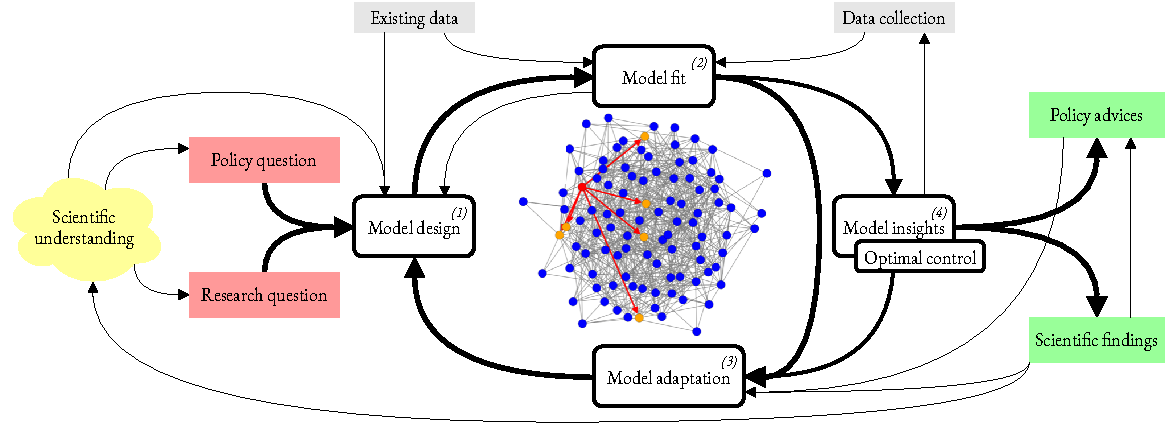
\includegraphics{fig/modeling_cycle}
  \caption[Processes for infectious disease modeling][-1\baselineskip]{Processes for  infectious disease modeling. The numerous feedback loops makes this procedure iterative. All boxes save for data collection were explored in this thesis. The central figure represents an agent-based model of disease transmission in a random graph (by Thomas Fry, a master student supervised during this thesis, with permission).}\label{fig:modeling}
\end{figure*}
\paragraph{Model fit} \textit{Fitting} conditions the model on the observed data. It allows one to infer unobserved states and parameters from reported quantities, such as the reduction of transmission during lockdown from hospitalization and deaths. A panel of methods for fitting a model to data has been developed. Usually computer-age statistical inference relies on thousands of model simulations to explore the high dimensional parameter and state spaces; each realization being evaluated against the data. The inner working of the fitting algorithms varies depending on the formal framework it is built on, but also on the numerous computational tools to make inference fast and precise. In this thesis, two classes of methods are used: Bayesian methods based on Markov chain Monte Carlo (MCMC) derivatives and frequentist Iterated Filtering (IF) methods. Fitting the model allows one to uncover previously unknown transmission parameters and unobservable states. As such, it requires a high-degree of care as inferred features may be caused by modeling artifacts instead of real epidemic features. Moreover results may misrepresent the uncertainties associated with the process and beware these methods fail more or less gracefully, thus it is possible to obtain results that seem reliable but are invariably wrong.
 
\paragraph{Model adaptation} An evaluation of the \textit{fit} of the model and the implications on the results is done by performing visuals and formal checks. More often than not, it is necessary to adapt either the fitting procedure or the model structure. It could be the inclusion or the removal of a process from the model. Or perhaps choosing to account for dynamics in a more or less explicit, detailed way. Models are lossy compressions of reality (from an information theory point of view), and choices on the processes to be included, and how to include them are the cornerstone of epidemiological modeling. Indeed despite its recent formalism, statistical inference remains an art, uncomfortably dependent on the practitioners, their backgrounds and their expectation\footnote{Multi-modeling studies -- where several modelers are tasked to answer the same question -- uncover the importance of the choices while performing statistical inference and mitigate the issues linked to opinionated model design.}. The cycle \textit{design}$\rightarrow$\textit{fit}$\rightarrow$ \textit{adapt} is then repeated until the predictive accuracy is satisfying for the goal of the exercise. 

\paragraph{Model insights}  Armed with a reliable model whose parameters and states are consistent with data and knowledge about an epidemic, it is now possible to answer the research questions. A model that reproduces observed dynamics may accurately represent epidemiological processes. It can be used as a substitute for experiments: it enables to simulate different intervention scenarios and to evaluate the impact of past or planned policies on a virtual system. This sets the range of expectations one can have with regard to the real world consequences of modeled policies. In some cases, the model is designed to replicate mechanistic relationships between the epidemiological processes, and several different models might be compared to identify which transmission routes are responsible for the observed dynamics.  Finally, the communication of model results ought to come with proper awareness of the limitations, as models are always incomplete and biased in reproducing the real epidemiological dynamics. It provides an additional opportunity for feedback towards an eventual adaptation of the model\cite{Heesterbeek:ModelingInfectiousDisease:2015}. 

\paragraph{Optimal control} Another application of epidemiological models explored in this thesis is their integration with optimal control methods to search for the \textit{best} intervention against infectious diseases. Optimal control methods are recent mathematical optimization procedures extending the calculus of variations to enable the derivation of control policies for dynamical systems. While technical adaptations are necessary to perform optimal control on epidemiological models, this rigorous framework identifies the most effective control measures under a set of operational constraints, discovering non-intuitive features and policies. These optimal interventions exploit every features of the complex interactions modeled, allowing to \eg best allocate a limited vaccine supply in space and time. Such tools, currently in their infancy and requiring accurate models, are promising as reasoning aid, uncovering another facet of disease transmission, and for the effective allocation of control resources in the fight against epidemics.



%\sidenote[][8\baselineskip]{Multimodeling studies and collaborative experiments strive to mitigate this issue by bringing together assumption and projections by different groups. See \eg \url{covid19forecasthub.org/community}}.

\section{Thesis aim and outline}
\begin{table*}[t]
\label{tab:allmodels}
\centering\small
\begin{tabularx}{\textwidth}{x{14mm}cccx{15mm}cx{15mm}p{30mm}}
\toprule
   \small{\textsc{Chapter}}     & Disease           & Compartments & Processes         & \small{$N_{\text{spatial}}$} & Fit       & Aim            & Reference\\
\midrule
4 & Cholera           & SEIR+B      & Stochastic    & --           & IF-like  & explain         & \tiny{\fullcite{Lemaitre:RainfallDriverEpidemic:2019}}\\
4 & Cholera           & SEIR+B      & Deterministic & --             & MCMC-like & explain        & \tiny{\fullcite{Lemaitre:RainfallDriverEpidemic:2019}}\\
5  & Cholera           & SEAIR$^3$+V & Stochastic    & 10        & IF-like   & project (scenarios)       & \tiny{\fullcite{Lee:AchievingCoordinatedNational:2020}} \\ \addlinespace
6  & \textsc{\textsc{covid}}-19 & SEI$^3$R+VH & Stochastic    & 3’000+    & MCMC-like & project (scenarios)        & \tiny{\fullcite{Lemaitre:ScenarioModelingPipeline:2021}} \\
7  & \textsc{\textsc{covid}}-19  & SEI$^3$R+H  & Stochastic    & --             & IF-like  & infer           & \tiny{\fullcite{Lemaitre:AssessingImpactNonpharmaceutical:2020}}\\
8  & \textsc{\textsc{covid}}-19  & SEIAR+VH    & Deterministic & 107       & MCMC-like & optimal\newline control & \tiny{\fullcite{Lemaitre:OptimizingSpatiotemporalAllocation:2021}}\\ 
\bottomrule
\end{tabularx}
\caption[Summary of the models described in this thesis]{Summary of the compartmental models described in this thesis.}
\end{table*}
The present thesis has been developed within the Swiss National Foundation project ``Optimal control of intervention strategies for waterborne disease epidemics (\textsc{snf} 200021–172578)’’. It initial goal was to develop a decision support system for the real-time design of optimal intervention strategies against cholera, which includes an operational forecasting tool coupled with an optimal control solver. This framework has been developed, albeit for \textsc{covid}-19 transmission in Italy, and is presented in \textsc{Chapter~6}. 


The work presented extensively builds on the ECHO laboratory expertise on the spatially-explicit modeling of cholera transmission\footnote[][2\baselineskip]{and waterborne diseases in general; see: \fullcite{Rinaldo:RiverNetworksEcological:2020a, Rinaldo:Reassessment20102011:2012}}. The group has developed over a decade a rainfall-mediated, spatially explicit cholera model that has inspired each of the other models presented in this thesis. The original model is presented in \textsc{Chapter~1} with a short introduction on the ancient disease that is cholera, and its sorrowful history.

Cholera is the focus of two additional chapters. The explanatory power of two existing models linking cholera transmission with rainfall are compared in \textsc{Chapter~2}, through the analysis of an outbreak in Juba, South-Sudan. In \textsc{Chapter~3}, a scenario planning estimation of the probability of eliminating cholera from Haiti through a mass vaccination campaign is presented; this work has been carried within the framework of a multi-modeling study with other groups, and input from the ministry of health of Haiti.
%\marginnote[-5\baselineskip]{Most bibliographic items and some additional precision are presented as margin notes for convenience. However, the full bibliography is included at the end of the thesis.}

The remaining chapters focus on \textsc{covid}-19. In \textsc{Chapter~4}, some facets of dealing with uncertainties from an emerging disease pandemic are uncovered, with a focus on a pipeline for scenario modeling that has been used to inform governments, in the United States and in other countries. 
Using data collected while participating in the \textsc{covid}-19 response, it was possible to estimate the impact of early interventions against \textsc{covid}-19 in Switzerland, this study is presented in \textsc{Chapter~5}. %\marginnote[-5\baselineskip]{Incidentaly, this organisation reflects the chronogical order of the work.}
And finally, \textsc{Chapter~6} presents how to integrate a spatially explicit epidemiological model for the Italian epidemic within an optimal control framework in order to discover the optimal strategy for vaccine allocation.




%\begin{fullwidth}
\chapter{A modelling oriented primer on cholera}
\end{fullwidth}
Cholera is an acute intestinal infection causing severe diarrhea that may lead to dehydration, and sometimes death. While the global burden of cholera is difficult to estimate as the majority of cases are not reported, it is estimated that 3 million cases and 95'000 deaths occurs every year in endemic areas (around 50 countries), with millions more at risk\cite{Ali:UpdatedGlobalBurden:2015}. Despite its household name, cholera belongs to the neglected tropical diseases group as our understanding of many important aspects of cholera clinical course and transmission is limited.
A political will to eliminate this ancient disease has recently arisen. The World Health Organization (WHO) initiated the Global Task Force for Cholera Control (GTFCC), who provides a concrete path towards the elimination of cholera by 2030\footnote{Elimination being defined as a 90\% reduction of cholera deaths/year, see \url{gtfcc.org} for more information.}. The general consensus is that to reach this goal in endemic countries, there must be substantial long-term improvements in safe water distribution systems, adequate sanitation and accessible hygiene education.  Moreover, in the event of a cholera outbreak, timely interventions such as vaccination campaigns are crucial to limit the spread of the disease, and proper medical treatment reduce the toll of the disease on communities. %With limited resources, public health officials face a number of challenging decisions, and a data driven decision support to guide the rational deployment of cholera control strategies is needed. Furthermore, on the road toward elimination, the need to setup context-specific tailored approaches appears. 
%The poorest of the poor
%most infected individuals are asymptomatic, i.e., they do not present symptoms, while other experience mild or severe symptoms.  %Since their mobility is not hindered, they become a vector of the infection. If not properly treated, cholera can kill children and adults within hours. 


\vspace{.7cm}
\section{History and epidemiology}
\begin{marginfigure}%[0\baselineskip]
%\centering
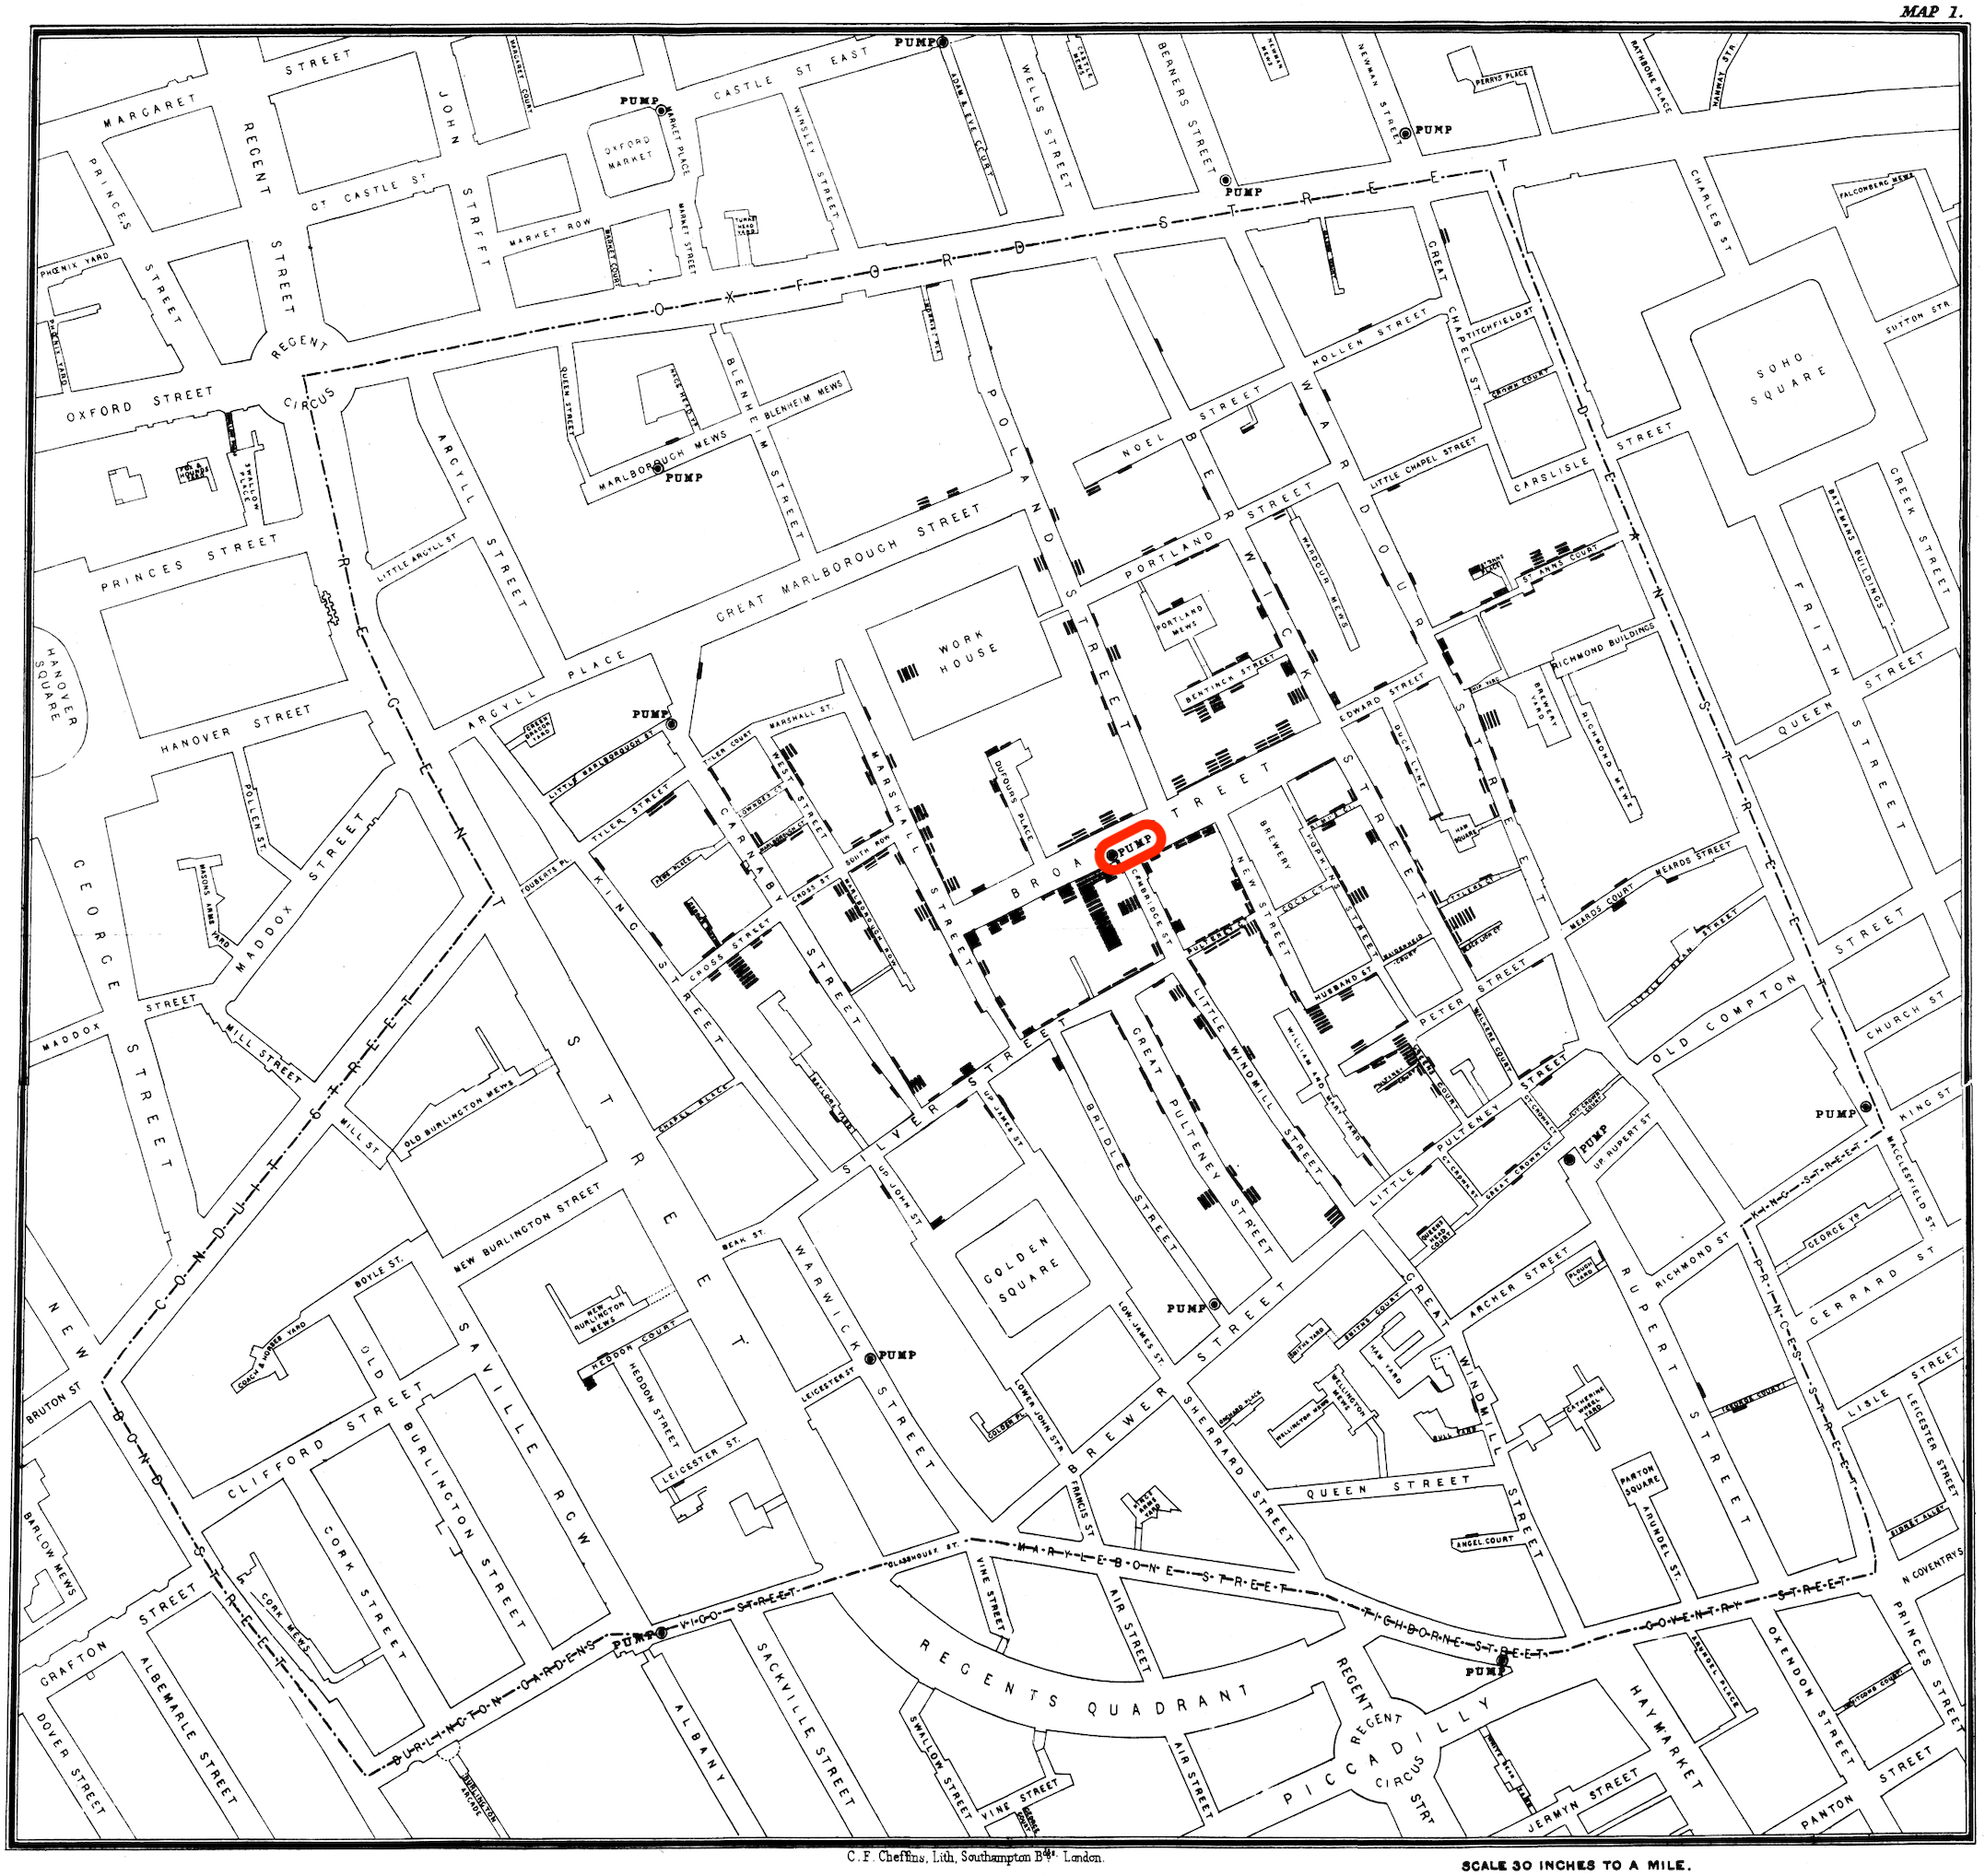
\includegraphics[width=\textwidth]{fig/snow-cholera-map_edit}
\margincaption[John Snow map of cluster cholera cases in London, 1854]{Original map by John Snow. Stacked rectangles represent cholera cases of the 1854 Broad Street outbreak. The work of John Snow conviced the authorities to close the water pump (circled in red), leading to a decrease in Mortality. Lithography by Charles Cheffins, in "\fullcite[p. 54]{Snow:ModeCommunicationCholera:1855}.}\label{johnsnow}
\end{marginfigure}
Humanity and cholera share a long history, with supposed mentions as early the 5th centurey \textsc{bce}. The disease became more widely know in the modern era. From 1817 to 1923, six successive pandemics -- all originated in the delta of the Ganges river, but taking different paths accross the world -- occured. Cholera spread around the world owning to the the nascent mobility, leaving 10s of millions dead accross countries and continents.  Scientific developments sped up during the third cholera pandemic (1846-60). In 1854, a cholera outbreak in Broad Street (Soho, London) was studied by physician John Snow and lead to an impressive early work in investigative epidemiology and public health. Analyzing the contamination pattern among residents, Snow postulated that cholera spread through water contaminated by an infectious agent, instead of foul air\sidenote[][-1\baselineskip]{At the time, the accepted mode of contamination for cholera and many other disease was through miasma, \textit{bad air} contaminated by organic matter. Chasing odor  justified urban amangement along streets and river banks in Paris and London. But also in Lausanne, where rivers Flon and Louve where covered in 1832 in response to a cholera outbreak. The cholera dish from Valais is a testimony of the strong impression cholera left on the Swiss.}.  Simultaneously, Italian microbiologist Filippo Pacini isolated the bacterium in Florence. Thirty years after Pacini, German scientist Robert Koch independently rediscovered the cholera pathogens after investigation in Egypt and India and first posited its causative relationship with the disease. Finally a hundred year later, Indian researcher Sambhu Nath De discovered the cholera toxin in 1959.

Throughout the seventh pandemic from 1961 onwards, cholera spread in several waves, through Asia in the 1960s, reachin Africa and the Middle East in the 1970s and the Americas in 1991\cite{Mutreja:EvidenceSeveralWaves:2011}. Improvement in sanitation and hygiene spared higher income country from disease, and cholera became a burden of the poorest of the Global South. Series of outbreaks (\eg Zimbabwe 2008, Haïti 2010, Yemen 2016), continuous transmission in endemic countries and millions at risks keeps this ancient disease a ongoing public health issue.

The span of this thesis was marked by a cholera outbreak in Yemen (2016--2021) -- an humanitarian crisis with 2.5M suspected cases and nearly 4'000 deaths -- an outbreak in Zimbabwe and flare up in Algeria in addition to seasonal outbreaks and endemic cholera transmission in the Asia and sub-saharian Africa.  But also by the last confirmed cases of cholera in Haiti in 2019.

While the number of cholera cases doubled from 2018 to 2019 to nearly a million, reported cholera death decreased to less than 2'000 in 2019, with Africa reporting lowest number since the 2000s. Haiti reported its last confirmed cholera cases in january 2019, bringing hope to cholera elimination from its last foothold in the Americas. Effort towards improvement of sanitary conditions and reactive vaccinations (24M doses of cholera vaccines were distribued in 2019) hope to bring these number down\footnote{see \fullcite{WHO:Cholera2019:2020} and previous \textit{Weekly Epidemiological Records} about cholera.}. 

In the following we highlight some relevant aspects about cholera transmission, while leaving some biological and medical features of cholera outside the scope of this thesis.


\section{Pathogen} 
\begin{marginfigure}[6\baselineskip]
\centering
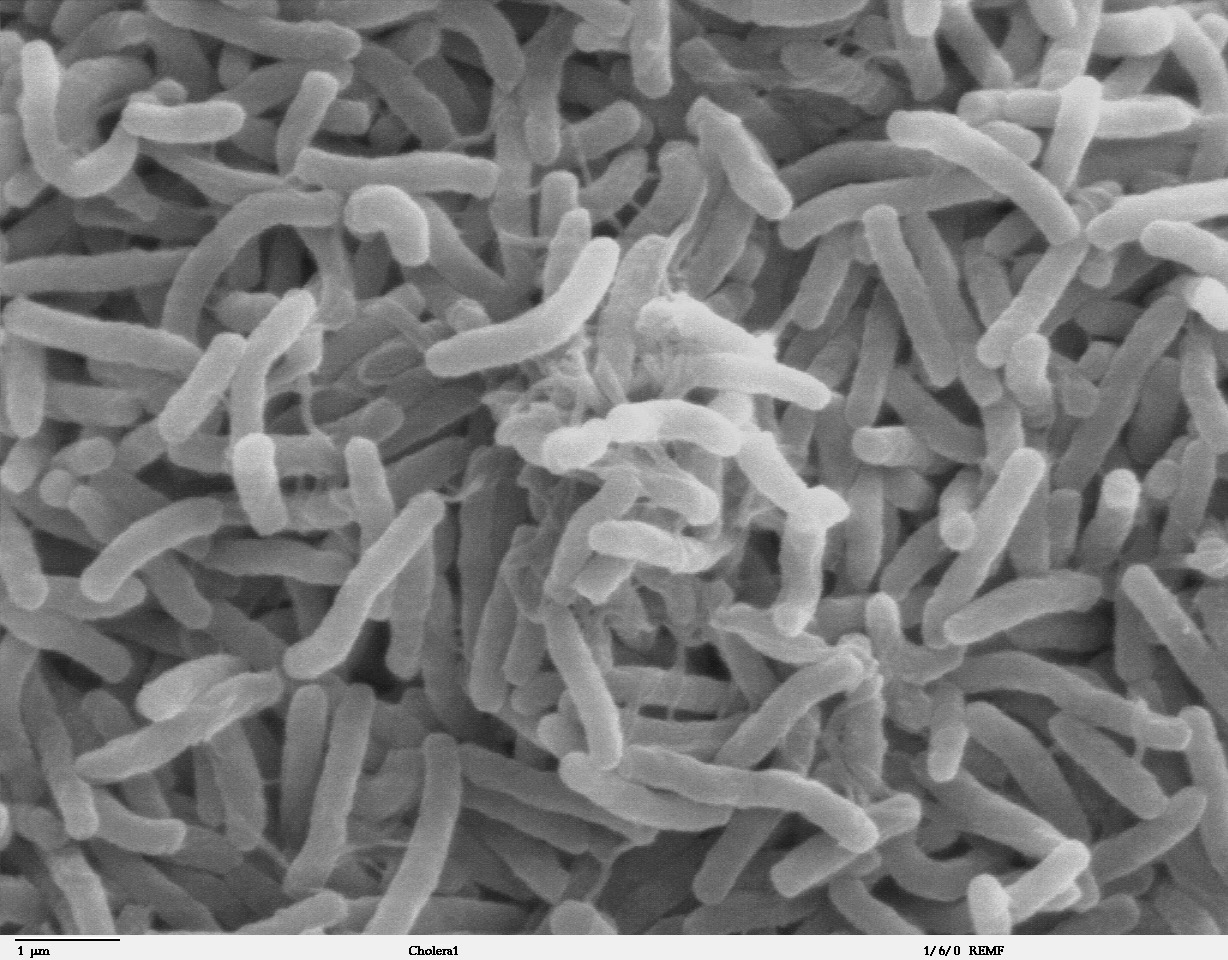
\includegraphics{fig/vibrio}
\margincaption[Vibrio cholerae bacteria]{Scanning electron microscope image of \textit{Vibrio cholerae} (Public domain image by Ronald Taylor, Tom Kirn, Louisa Howard).}
\label{rain}
\end{marginfigure}
\paragraph{Pathogen} Cholera is an infection caused by a waterborne bacteria: the \emph{Vibrio cholerae}. While many serogoups of \emph{V. cholerae} can secrete the cholera toxin reponsible for massive watery diarrhea, only serogoups O139 and O1 are responsible for disease epidemics. O1 is causing most recent epidemics, and is divided in two biotypes: Classical O1 and El Tor, which are both divided into three serotypes: Ogawa, Inaba and the rare Hikojima\cite{Kaper:Cholera:1995}. Cholera classification has its importance as it affects many epidemiological characteristic \eg, El Tor survives longer in water and has an higher asymtomatic/symptomatic ratio\cite{WHO:CholeraVaccinesWHO:2017}. The current cholera pandemic is mainly caused by El Tor, while the Classical derivative caused previous fifth and sixth pandemic and is now limited to the Gange delta\cite{Nair:CholeraDueAltered:2006}. 

 \paragraph{Environmental reservoir}  \textit{V. cholerae} exists as natural habitant in some aquatic ecosystem, in particular in brackish waters and estuaries. There is no marine host, but complex ecological association processes take place in the aquatic medium, and natural genetic transformation is enabled by chitin, the polymer constituting the crustacean exoskeleton\cite{Reidl:VibrioCholeraeCholera:2002,Meibom:ChitinInducesNatural:2005}. There is no concensus on how long \textit{V. cholerae} remains infectious in water and under which conditions it is able to reproduce\cite{Mavian:ToxigenicVibrioCholerae:2020}. In cholera epidemics, it is difficult to isolate the role of the natural cholera reservoir from freshly introduced \textit{Vibrios} from the feces of an infected person, though the later is suspected to drive  transmission during outbreaks.

\paragraph{Climatic Drivers} Cholera expresses marked seasonality patterns that takes different shapes in accross setups. A complex and unclear association between precipitation and cholera infections has been put forward in many research works. After hurricane Matthew and heavy rainfall in October 2016, a cholera flare-up started from low transmission in Haiti\cite{Pasetto:RealtimeForecastingCholera:2018}. Similarly, cholera in many African countries follows a seasonal trend, with the epidemiological curve raising during the rainy season\cite{Baracchini:SeasonalityCholeraDynamics:2017}.  Rainfalls might play a major role in water contamination, for instance through the washout of open-air defecation and raw sewage circulation in the environment. A litterature review of the relationship between cholera and rainfall is provided in the next chapter. Temperature, water acidity, sunlight and other environemental factors have also been shown to affect the survival and reproduction of \textit{V. cholerae} in water bodies. Hence macro climate phenomena such the El Niño Southern Oscillation have been associated with changes in transmission, even if no causal link could be established\cite[-2\baselineskip]{Pascual:CholeraDynamicsNinoSouthern:2000}\footnote{Marc Lipsitch and Cécile Viboud beautifully describe the difficulty evaluating the environmental factors in disease transmission, writing for influenza: "This potpourri of possible mechanisms places us in a kind of Popperian purgatory, in which data in support of every hypothesis exist, yet none of the hypotheses has been subjected to tests that are rigorous enough to reject it." in \fullcite{Lipsitch:InfluenzaSeasonalityLifting:2009}}.

\section{Cholera in the human} 
\paragraph{Disease} An human host becomes infected through the ingestion of a critical dose of \emph{V. cholerae}\shortcite{Kaper:Cholera:1995,Nelson:CholeraTransmissionHost:2009}. The susceptibility depends on many factors such as gastric acidity and age, with under 5 much more likely to become infected\cite{Sack:Cholera:2004}. \textit{V. cholerae} colonize the small intestine for an incubation period lasting 12 hours to 5 days\cite{Azman:IncubationPeriodCholera:2013} before symptoms. Then, a wide range of outcomes are possible. Most of the time the infection is inapparent, resulting in asymptomatic individuals. On the other end of the spectrum severe infection (or \emph{cholera gravis}), caracterized by vomiting and profuse rice water diarrhea, occurs in 1\% to 15\% of the cases. Many stages of mild infections lie between asymptomatics and severe infections. Unless tested in a laboratory, symptoms are indistinguishable  from those of numerous other infections causing diarrhea\footnote{\fullcite{King:InapparentInfectionsCholera:2008};  \fullciteshortb{Kaper:Cholera:1995, Nelson:CholeraTransmissionHost:2009}; \fullcite{vandeLinde:ObservationsSpreadCholera:1965,Mccormack:CommunityStudyInapparent:1969}}.  The severity of illness correlates with the quantity of \textit{V. cholerae} ingested\cite{Brouwer:DoseresponseRelationshipsEnvironmentally:2017}, and depends on the cholera strain and personal characteristics, immunity, pregnancy, blood type\cite{WHO:CholeraVaccinesWHO:2017,Azman:IncubationPeriodCholera:2013}, ...%Table 1 for a review of individual data studies.
Treatment is crucial: severely infected individuals migth loose up to 20 litres of water through diarrhea a day and may die within hours. If left untreated, natural mortality reaches up to 60\% but proper therapy lowers mortality below 1\%\cite{Luquero:MortalityRatesCholera:2016}.

\paragraph{Shedding and transmission} The intensity of the bacterial shedding varies with the intensity of the infection. It is estimated to range from $10^3$ to $10^{9}$ vibrios per gram of stool for asymptomatic infected and severely infected individual respectively\shortcite{Nelson:CholeraTransmissionHost:2009}. Similarly, the duration of the shedding period typically ranges from a day up to two weeks\shortcite{Nelson:CholeraTransmissionHost:2009, Kaper:Cholera:1995}.
Transmission occurs along the fecal-oral route (consumption of contaminated water or food, contact with fomites), but contamination is also possible from aquatic reservoirs, through water or seafood. Freshly shed \textit{Vibrios} may be in an hyperinfectious state, which could be of great importance in driving epidemic transmission\cite{Butler:CholeraStoolBacteria:2006}. The principle mechanism of transmission is the intake of water contaminated by the untreated diarrheal discharge of other infectious individuals.
Asymptomatic individuals remains mobile and shed bacteria, thus may be of importance for cholera dissemination.

\paragraph{Human mobility and hydrological transport} Spatial spread of cholera outbreaks may occurs through two networks. \textit{V. Cholerae} may be transported through the river network. A example is the spread of the 2010 Haiti epidemic along the Artibonite river\cite{Piarroux:UnderstandingCholeraEpidemic:2011}. Human mobility also plays a major role in the spreading of the infections possibly due to the large number of asymptomatic that transport and disperse cholera across a country or even worldwide.  Indeed also in Haiti, cholera was brought into Haiti by infected United Nations peacekeepers\cite{Piarroux:UnderstandingCholeraEpidemic:2011}. %However, mobility, especially in humanitarian crisis situations often associated with cholera, remains difficult to predict\cite{Lu:PredictabilityPopulationDisplacement:2012,Riley:LargeScaleSpatialTransmissionModels:2007,Bengtsson:ImprovedResponseDisasters:2011,Rebaudet:DrySeasonHaiti:2013}.

\paragraph{Immunity} Infected individuals that recover from the infection are immunized against \textit{V. cholerae}  of the same serogroup. The duration of acquired immunity is difficult to estimate, and depends on many factors. Acquired immunity has been reported to range from few months to several years \footnote{Most current estimages ranges from 2 to 10 years.}, possibly depending on the virulence of the infection\cite{Levine:DurationInfectionDerivedImmunity:1981,Kaper:Cholera:1995,Woodward:CholeraReinfectionMan:1971,Glass:SeroepidemiologicalStudiesEI:1985,Clemens:BiotypeDeterminantNatural:1991,Leung:ProtectionAffordedPrevious:2021}.

\subsection{Cholera Control} 
Cholera interventions may be preventive or concern the treatment of infected individual. Treatment plays an important role in reducing the reproduction number of the epidemic and mainly consists of:
\begin{description}
\item[Oral (or Intravenous) Rehydratation Therapy] The main treatement for cholera consists of replacing fluids as fast as they are lost. Despite its simplicity, it is very effective in reducing mortality. Fluids with the same electrolyte composition must be administred\cite{Kuhn:GlucoseNotRiceBased:2014}.  Rehydratation is usually done in treatment centers, but may take place at the patient home. This differentiation might determine if stools contribute to the infection cycle or are properly disposed.
\item[Antibiotics] reduce the severity and the duration of the infection. WHO recommends their use only for the most severe cases as antibiotic resistance of \emph{V. cholerae} is raising worldwide\cite{Sack:GettingSeriousCholera:2006}.
\end{description}

Prevention measures may be carried out before and during the outbreak, and are described below.

\paragraph{Surveillance \& Reporting} During an outbreak, surveillance consists of the timely reporting of new cases. In many countries where outbreaks occurs annually during the rainy season, the observation of past epidemics provides insight on the severity and timing of the infection that can be used for preparation\cite{Baracchini:SeasonalityCholeraDynamics:2017}. Environmental surveillance, monitoring for \textit{V. Cholerae} in the water, is also possible. However, never has \textit{V. Cholerae} been found in the environment before an epidemic. 
Without laboratory equipement, it is impossible to distinguish cholera from another pathogen in a patient with acute watery diarrhea. The has been an effort to standardize the clinical definition of a suspected cholera case, which varies between countries and during outbreaks. A suspected case combine acute watery diarrhea and severe dehydration, the latter condition being dropped in case of outreak. This diagnosis can be validated using rapid diagnosis tests (RTDs), with a pretty high sensibility but low sensitivity. Precise indentification is obtained through culture, the current gold standard\footnote{\fullcite{Camacho:CholeraEpidemicYemen:2018} and \fullcite{CDC:DiagnosisDetectionCholera:2018}}. RTDs and culture are not always available, especially during an outbreak.  As a consequence, over-reporting during an outbreak situation is likely, as is under reporting as transmission settings might be isolated or plagued with conflicts, natural disaster. WHO guidelines recommend that, when a patient enters a treatment center, his name, address, sex, age (over or below 5) and symptoms are recorded\cite{WHO:FirstStepsManaging:2010}. % https://apps.who.int/iris/bitstream/handle/10665/334241/WER9537-eng-fre.pdf?ua=1 end, and https://www.cdc.gov/cholera/diagnosis.html

\paragraph{WaSH} Water, Sanitation and Hygiene (WaSH) is a broad term that includes many intervention strategies that are key to the long term elimination of cholera. The improved sanitary conditions have been the main factor that led to cholera elimination  in first world countries. WaSH is divided into short and long term measures. Short term strategies involve sterilization, decontamination, hand washing, education sessions and water purification and filtering (chlorination, ...)\cite{Rebaudet:NationalAlertresponseStrategy:2018,Fewtrell:WaterSanitationHygiene:2005}. Long-term sanitation strategies involve the construction of infrastructures for fecal sludge management, sewage systems, toilets and access to safe water sources. From a modeling point of view, WaSH reduces exposure (water purification, sari filtration) and shedding (sewage and fecal sludge management). By its nature and its delayed, longterm effects, WaSH improvement is difficult to quantify in modeling framework.

\paragraph{Vaccination} is a safe and effective way to protect individuals from cholera, and to reduce the propagation of the epidemic. It can be used in a preventive or reactive way. Several vaccine exists for cholera, with different characteristics. As of today, two main oral cholera vaccines (OCVs) are used in vaccination campaigns around the world: WC-rBS and BivWC\footnote[][-3\baselineskip]{An other vaccine, Vaxchora, was recently approved by the FDA, mostly for travelers.}. The main characteristics of these two vaccines are shown in Table~\ref{tab:vacc}.

\begin{table}[h]
\centering\small
\label{tab:prior}
\begin{tabular}{lp{40mm}p{40mm}}
\toprule
Generic Name &  BiWC & WC-rBS\\ 
\midrule
Commercial name   &  mORCVAX, Shanchol,  Euvichol, Cholvax & Dukoral  \\
Target strain O1 &   yes (classical, El Tor, Ogawa, Inaba)& yes (classical, El Tor, Ogawa, Inaba), also  target a cholera toxin  \\
Target strain O139   &  yes &      no     \\
Doses   &  2 doses, 2 weeks apart & 2 doses (3 for children) 1--6 weeks apart  \\
%Vaccine Efficacy & 58\% &  \\
Field Effectiveness  & between 37\% and 87\% for two years & 78\% protection 1--6 months after vaccination\\
Age   &  $>$ 1 year & $>$ 2 year      \\
Usage & Mass vaccination, Global OCV stockpile, 25M doses administered & Mainly for travelers ($>$ 1M doses administered)\\
Protection length & 3 years (1 dose: short term protection) & 2 years\\
Constraints & -- & needs buffer solution\\
Price per dose & 1.85\$ & 5.25\$ \\ 
Usage & Since 1998 in most recent outbreaks & Between 1997 and 2009 in Uganda, Tanzania, Indonesia,~... \\
\bottomrule
\end{tabular}
\caption[Characteristic of currently available vaccines][-2\baselineskip]{Characteristic of currently available vaccines. The proposed value for field effectiveness, along with vaccine efficacy (not shown here) is really difficult to evaluate, cannot be written in a simple way without omitting crucial information. A good review of research on cholera vaccine is the WHO Position paper on cholera vaccines~\fullcite{WHO:CholeraVaccinesWHO:2017}. See also~\textcite{WHO:BackgroundPaperWholeCell:2017,Azman:PopulationLevelEffectCholera:2016,Luquero:FirstOutbreakResponse:2013,WHO:BackgroundPaperIntegration:2009,Luquero:UseVibrioCholerae:2014,Qadri:EfficacySingledoseRegimen:2018,Bi:ProtectionCholeraKilled:2017,Azman:ImpactOneDoseTwoDose:2015,Tohme:OralCholeraVaccine:2015}.}
\label{tab:vacc}
\end{table}

 Vaccine can either be administered in a targeted fashion or to whole populations in mass vaccination campaigns. Despite effort to build a worldwide vaccine stockpile, demand for cholera vaccine vastly exceeds supply\cite[-1\baselineskip]{Parker:AdaptingGlobalShortage:2017a,Seidlein:PreventingCholeraOutbreaks:2018}.


\section{Cholera Modeling}
Cholera modeling has received renewed a lot of attention during the 2010 Haiti outbreak, and serves different purposes. 
Most of recent modeling efforts focus on phenomenological (or statistical) models with different degrees of deterministic processes\shortcite[-2\baselineskip]{Azman:UrbanCholeraTransmission:2012,Finger:PotentialImpactCasearea:2018,Camacho:CholeraEpidemicYemen:2018,Lessler:MappingBurdenCholera:2018,Koelle:DisentanglingExtrinsicIntrinsic:2004}. Mechanistic cholera models embed uncertainties into their parameter distribution, and differ in the way they account for the epidemiological processes\shortcite{Kirpich:ControllingCholeraOuest:2017,Tuite:CholeraEpidemicHaiti:2011,Chao:VaccinationStrategiesEpidemic:2011,Kirpich:CholeraTransmissionOuest:2015}. Most cholera models are spatially implicit, however there have been a number of attempts to describe the spatial spread of the epidemic. For example, Andrew and Basu used an approach with isolated nodes and independent transmission parameters in each node\shortcite{Andrews:TransmissionDynamicsControl:2011}.

\subsection{ECHO's cholera model}
A spatially-explicit model has been developed at ECHO in the past 10 years \parencite{Bertuzzo:SpacetimeEvolutionCholera:2008}. It has been used for studies on the dynamics of several cholera epidemics, such as in South Africa in 2000 \parencite{Mari:ModellingCholeraEpidemics:2012}, Senegal in 2005, Haiti from 2010 to 2019 \parencite{Bertuzzo:PredictionSpatialEvolution:2011,Bertuzzo:ProbabilityExtinctionHaiti:2016}, Democratic Republic of the Congo from 2004 to 2011 and many others\cite{Finger:PotentialImpactCasearea:2018}.  
We present here a complete formulation of the model, including patterns and effectiveness of vaccinations, human and hydrological mobility \parencite{Bertuzzo:ProbabilityExtinctionHaiti:2016,Pasetto:RealtimeForecastingCholera:2018}. This model has inspired to a various degree all the other model described in this thesis.

The model is a variation of the SIR model introduced first by Kermack and McKendrick\cite{Kermack:ContributionMathematicalTheory:1927}, with additional compartments for the vaccinated individuals and the bacteria concentration in the environment.

The model subdivides the area potentially concerned by the epidemic into $n$ sub-regions. The sub-regions, defined by political boundaries or geomorphological features (like watersheds\cite{Bertuzzo:ProbabilityExtinctionHaiti:2016}), are represented as connected nodes. The $n$ nodes represent $n$ human communities having population size $H_i$, $i=1,\dots, n$. 

At time $t$ and for each node $i$, the individuals in the node can be grouped into six compartments:

\begin{itemize}
\item $S_i(t)$: susceptible individuals  have no immunity, and may enter in contact with the bacteria and become infected (symptomatic or not),
\item $I_i(t)$: infected individual shed bacteria into the community reservoir,
\item $R_i(t)$: recovered are temporally immune, and don't participate in disease transmission,
\item $V^S_i(t)$: vaccinated susceptible,
\item $V^I_i(t)$: vaccinated infected,
\item $V^R_i(t)$: vaccinated recovered.
\end{itemize}

In addition, the model considers the bacterial concentration of \textit{V.~cholerae} in the water reservoir of the community, $B_i(t)$. The $n$ nodes are connected by both human mobility and pathogen transport through water.

Individuals commute from node $i$ to node $j$ with probability $Q_{ij}$. Bacteria are transported along the river network from node $i$ to node $j$ with probability $P_{ij}$.

The cholera dynamics are described by the following set of coupled ordinary differential equations:
\begin{fullwidth}

\begingroup
\allowdisplaybreaks
\begin{eqnarray}
\frac{dI_i}{dt} &=& \sigma F_i(t) S_i - (\gamma + \mu + \alpha) I_i \label{eq:I2}\\
\frac{dR_i}{dt} &=& (1-\sigma) F_i(t) S_i + \gamma I_i - (\rho + \mu+\frac{\nu_i(t)}{S_i+R_i}) R_i \label{eq:R2}\\
\frac{dV^S_i}{dt} &=& \nu_i(t) \frac{S_i}{S_i+R_i}-\mu V^S_i \label{eq:VS2}\\
\frac{dV^I_i}{dt} &=& \sigma (1-\eta) F_i(t) V^S_i - (\gamma + \mu + \alpha) V^I_i \label{eq:VI2}\\
\frac{dV^R_i}{dt} &=& \nu_i(t) \frac{R_i}{S_i+R_i} + (1-\sigma) (1-\eta) F_i(t) V^S_i + \gamma V^I_i - (\mu+\rho_v) V^R_i \label{eq:VR2}\\
\frac{dB_i}{dt} &=& - \mu_B B_i +\frac{p}{W_i}\left[1 + \phi J_i(t) \right] \left((1-m)(I_i +V_i^I)+m \sum_{j=1}^n Q_{ij} (I_j +V_j^I)\right)-  l \left( B_i - \sum_{j=1}^n P_{ji} \frac{W_j}{W_i} B_j \right)
\end{eqnarray}
\endgroup
\end{fullwidth}
where the population~$H_i$ of each node is assumed to be at demographic equilibrium, thus $S_i=H_i-I_i-R_i-V_i^S-V_i^I-V_i^R$.

The force of infection, i.e the rate at which individual enters in contact with the diseases, is written as:

\begin{equation}
F_i(t) = \beta \left[ (1 - m) \frac{B_i}{K + B_i} + m \sum_{j=1}^n Q_{ij} \frac{B_j}{K + B_j} \right].
\label{force}
\end{equation}

The parameter~$\beta$ represents the maximum exposure rate, which may decrease in time due to awareness of the population on the cholera transmission factors\cite{Bertuzzo:ProbabilityExtinctionHaiti:2016}. The fraction $B_{i}/(K+B_{i})$ is the probability of becoming infected due to the exposure to a concentration~$B_i$ of \textit{V.~cholerae}, $K$ being the half-saturation constant\cite{Codeco:EndemicEpidemicDynamics:2001}. The force of infection in a given node depends for a fraction ($1-m$) to the local concentration of \textit{V.~cholerae}, $B_i$, while the remaining fraction $m$, represents the community-level probability that individuals travel outside their node, accounts for the contribution of the concentration~$B_j$ of the remote communities. 
The human mobility is accounted with the matrix $Q_{ij}$ representing the probabilities that an individual living in node $i$ reaches~$j$ as a destination. Because of human mobility, a susceptible individual residing at node $i$ can be exposed to pathogens in the destination community $j$. 
In the lack of detailed mobility data,  the probabilities~$Q_{ij}$ can be estimated through a gravity approach\cite{Erlander:GravityModelTransportation:1990} to model human mobility:

\begin{equation}
Q_{ij} = \frac{H_j e^{-d_{ij}/D}}{\sum_{k \neq i}^n H_k e^{-d_{ik}/D}} \, ,
\label{eq:mob}
\end{equation}
where the attractiveness of node~$j$ depends on its population size $H_j$, while the deterrence factor is assumed to be dependent on the distance~$d_{ij}$ between the two communities via an exponential kernel (with shape factor~$D$).  

Due to the contact with contaminated water, a fraction $\sigma$ of the infected individuals develops symptoms, passing from compartment $S$ to $I$. The remaining fraction~$(1-\sigma)$ does not develop symptoms, does not contribute to the disease transmission, and is considered temporally immune, thus passing from compartment $S$ to $R$.  Symptomatic infected individuals recover at a rate~$\gamma$, or die due to cholera or other causes at rates~$\alpha$ or $\mu$, respectively.
Recovered individuals lose their immunity at rate~$\rho$, thus passing from compartments $R$ to $S$, or die at a rate~$\mu$.  % TODO Too many times property.

The environmental concentration of \textit{V.~cholerae} at a node $i$ may increase due to both human mobility and to hydrologic dispersion. Human contributions depends from a fraction $1-m$ on the local infected individuals and form a fraction $m$ on the symptomatic infected individuals moving according to the mobility model. The increase in bacteria concentration is modeled with the rate~$p/W_i$, where $p$ is the rate at which bacteria excreted by an infected individual reach and contaminate the local water reservoir of volume $W_i$ (assumed to be proportional to population size, i.e., $W_i=c H_i$ as in\textcite{Rinaldo:Reassessment20102011:2012}) and $\mu_B$ is the rate of decay of \textit{V.~cholerae}. Bacteria undergo hydrologic dispersal at a rate~$l$: pathogens travel from node~$i$ to~$j$ with probability $P_{ij}$, which is assumed to be one if node~$j$ is the downstream nearest neighborhood $i$, and zero otherwise. In order to express the worsening of sanitation conditions caused by rainfall-induced runoff, when relevant, which causes additional pathogen loads to enter the water reservoir due to effects such as the overflow of pit latrines and washout of open-air defecation sites\cite{Gaudart:SpatioTemporalDynamicsCholera:2013}, the contamination rate $p$ is increased by the rainfall intensity $J_i(t)$ via a coefficient $\phi$\cite{Rinaldo:Reassessment20102011:2012,Righetto:RainfallMediationsSpreading:2013}. By introducing the dimensionless bacterial concentrations $B_i^*=B_i/K$,  it is possible to group three model parameters into a single ratio $\theta=p/(cK)$\cite{Bertuzzo:SpacetimeEvolutionCholera:2008}.

The estimation of the local incidence is computed integrating over the new symptomatic individuals,

\begin{equation}
\frac{d C_i}{dt} \ = \ \sigma F_i S_i  \, , \label{eq:C}
\end{equation}

During the vaccination campaign, OCV doses are assumed to be distributed with rate $\nu_i(t)$ to susceptible and recovered individuals, which enter the compartments $V^S$ and $V^R$. As the OCV provides a partial immunity having efficacy $\eta$, $0\leq \eta \leq 1$, vaccinated susceptibles ($V^S$) can become infected ($V^I$) through a decreased force of infection of a factor $(1-\eta)$ with respect to non-vaccinated individuals. Vaccinated infected individuals behave exactly like infected ones, but are placed in a different compartment to exclude them from future vaccination campaigns. After recovering at  rate $\gamma$, they lose their vaccine protection at rate $\rho_{v}$.


%ffective targeted interventions 
%could eliminate 50\% of the region’s cholera by covering 35·3 million people (95% CrI 26·3 million to 62·0 million),
%which is less than 4\% of the total population\cite{lessler_mapping_2018} + hotspot vs optimal strategiy
%hotspot\cite{azman_micro-hotspots_2018}

%The Dry Season in Haiti: a Window of Opportunity to Eliminate Cholera\cite{rebaudet_dry_2013}

%\paragraph{Interventions design} The planning of the interventions described above is difficult to establish, as many factors enter into consideration including logistical and political constraints. Expert opinion is a valuable resource, however its use during outbreaks is not necessarily feasible and a consensus on strategy choice does not always emerges\cite{Cyranoski:CholeraVaccinePlan:2011}. Moreover, the global vaccine shortage\cite{Parker:AdaptingGlobalShortage:2017a,Seidlein:PreventingCholeraOutbreaks:2018} calls for an optimal use of current resources. Mass vaccination campaigns should be conducted only when strictly necessary. Case-area targeted interventions (CATIs) are an effective way of mitigating an outbreak while saving scarce resources. However, the optimal allocation in time and space of such interventions is strongly context-dependent which hinders the definition of general guidelines\cite{Eubank:ModellingDiseaseOutbreaks:2004,Finger:PotentialImpactCasearea:2018,Seidlein:PreventingCholeraOutbreaks:2018,Azman:MicrohotspotsRiskUrban:2018,Lessler:MappingBurdenCholera:2018,Rebaudet:DrySeasonHaiti:2013}. 

%This thesis will explore the possibility to apply optimal control for  both short- and long-term interventions across all scales. 
 % 1
%\begin{fullwidth}
\chapter[Rainfall as a driver of epidemic cholera: Comparative assessments of the effect of intra-seasonal precipitation events]{Rainfall as a driver of epidemic cholera:\\Comparative assessments of the effect of\\intra-seasonal precipitation events}\label{ch:cholera-rainfall}

The correlation between cholera epidemics and climatic drivers, in particular seasonal tropical rainfall, has been studied in a variety of contexts. Several mechanistic models have included rainfall as a driver of cholera transmission by focusing on two possible pathways: either by increasing exposure to contaminated water (\eg due to worsening sanitary conditions during water excess), or by increased water contamination with freshly excreted bacteria (\eg due to washout of open-air defecation sites or overflows). In this chapter, the explanatory power of these different model structures is assessed by formal model comparison using deterministic and stochastic models of the type susceptible-infected-recovered-bacteria (SIRB). The incorporation of rainfall effects is generalized using a nonlinear function that can increase or decrease the relative importance of large precipitation events. The modelling framework is applied on the daily epidemiological data collected during the 2015 cholera outbreak in Juba, South Sudan. This epidemic is characterized by a particular intra-seasonal double peak of incidence in apparent relation with particularly strong rainfall events. Results suggest that rainfall-based models in both their deterministic and stochastic formulations outperform models that do not account for rainfall. In fact, classical SIRB models are not able to reproduce the second peak, suggesting it was rainfall-driven. Moreover stronger support is found for rainfall acting on increased exposure rather than on exacerbated water contamination. Although these results are context-specific, they stress the importance of a systematic and comprehensive appraisal of transmission pathways and their environmental forcings when embarking in the modelling of epidemic cholera.

This section is adapted from:
\longfullcite{Lemaitre:RainfallDriverEpidemic:2019}.%\footnote[][-4\baselineskip]{JL, JP-S and DP developed the numerical tools required for the comparison. JL and DP conducted the numerical analyses for the deterministic model while JP-S conducted the numerical analyses for the stochastic model. AR and DP designed the framework for this study. JFW provided the epidemiological data. CS analyzed the data and prepared the model input. All authors contributed to the discussion of the results and writing of the manuscript.}.
\end{fullwidth}

\section{Rainfall and the transmission of cholera}\label{sec:rainfall-cholera-transmission}
Two main exposure pathways fuel cholera transmission across endemic and epidemic settings.
First, an \textit{indirect} exposure occurs from consumption of water contaminated by untreated sewage%\footnote{discovered by John Snow during the 1854 Broad Street cholera outbreak\fullcite{Snow:ModeCommunicationCholera:1855}}
; rainfall and the ensuing hydrologic transport processes might play a role in water contamination, for instance through the washout of open-air defecation sites and sewage circulation in the environment.
Alternatively, \textit{Direct}, or human-to-human exposure occurs when the bacteria is transmitted from an infectious individual directly to a susceptible one, for example via contaminated food or fomite. In this case, environmental factors do not play a major role, except for transmission changes due to behaviour modifications.
The mechanism behind the transmission of cholera has been postulated to be a combination of environmentally-mediated and direct exposures\shortcite[-4\baselineskip]{Sugimoto:HouseholdTransmissionVibrio:2014,Bi:MicroscaleSpatialClustering:2016,Lessler:MeasuringSpatialDependence:2016,Rinaldo:ModelingKeyDrivers:2017}.
% Cholera and climate (STOP)
\paragraph{Cholera and Rainfall} The relationship between different climatic and environmental factors and the transmission of cholera has long been studied. Works linking cholera outbreaks to anomalies in the El Niño Southern Oscillation\shortcite[-2\baselineskip]{Colwell:GlobalClimateInfectious:1996, Pascual:CholeraDynamicsNinoSouthern:2000, Hashizume:DifferentialEffectIndian:2013}  have paved the way for a new field in epidemiological research.
 \begin{marginfigure}[-1\baselineskip]
\centering
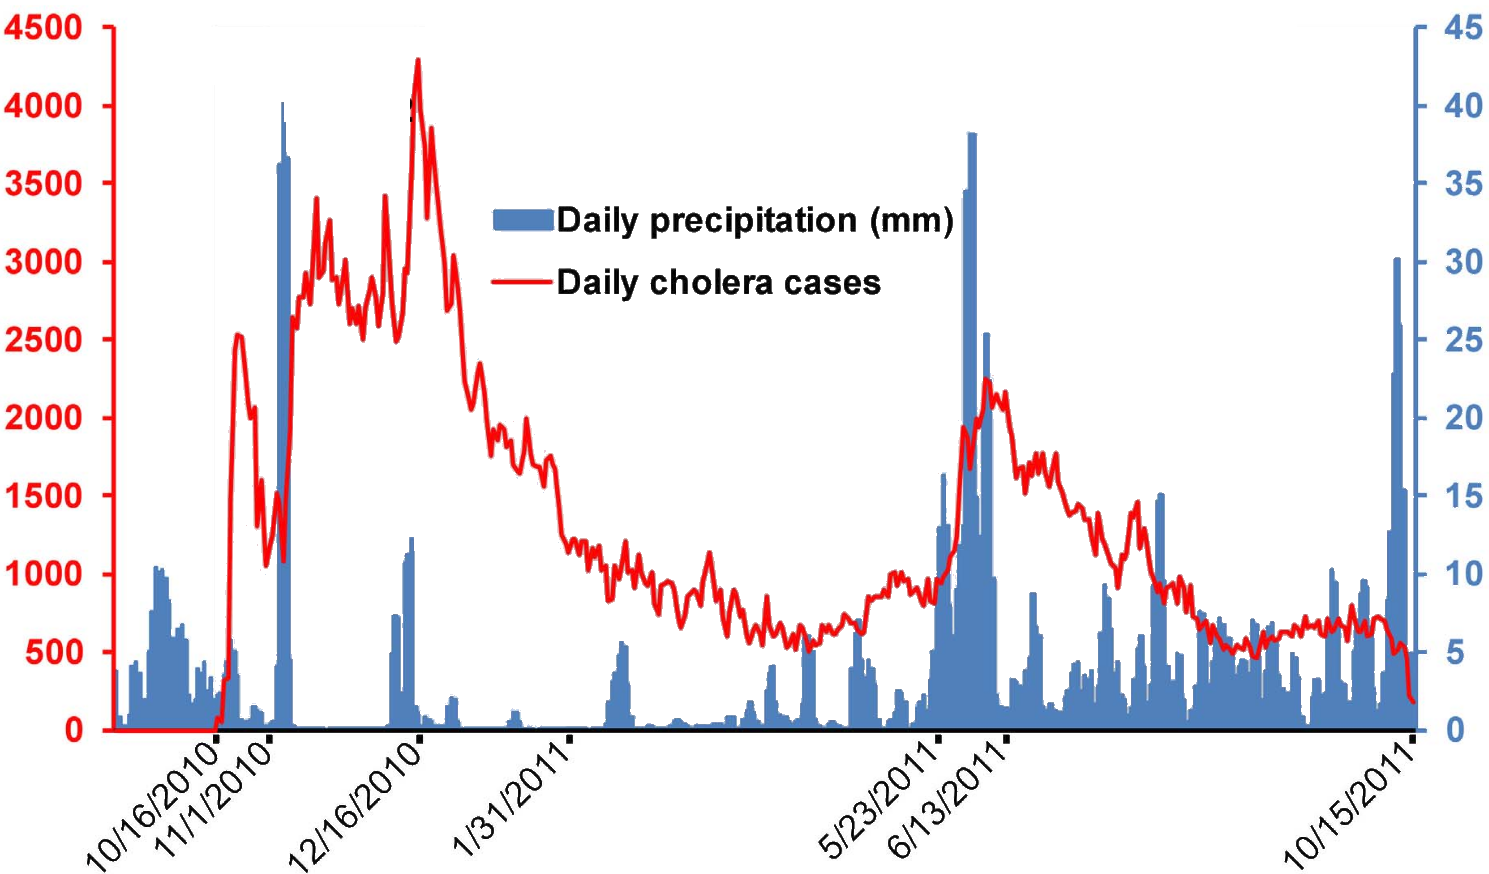
\includegraphics{fig/cholera-rainfall.png}
\margincaption[Similarities between daily cholera incidence and rainfall in Haiti]{\footnotesize Daily cholera cases (red) and daily rainfall (blue) in Haiti from September 15, 2010 to October
16, 2011. It highlights the visual correlation between heavy rainfall event and cholera outbreaks. Adapted from \fullcite{Gaudart:SpatioTemporalDynamicsCholera:2013}.}
\label{fig:rain}
\end{marginfigure}
 Previous studies have highlighted the role of climatic drivers on cholera dynamics, mostly focusing on climate change effects on disease spread\shortcite{Rinaldo:ModelingKeyDrivers:2017,Hashizume:EffectRainfallIncidence:2008,Magny:CholeraOutbreakSenegal:2012,Rodo:ClimateChangeInfectious:2013,Ramirez:NinoClimateCholera:2016,Vezzulli:ClimateInfluenceVibrio:2016} or on the impacts of spatial and temporal heterogeneities\shortcite{Reiner:HighlyLocalizedSensitivity:2012, Baker-Austin:EmergingVibrioRisk:2013, Vezzulli:OceanWarmingSpread:2013, Cash:CholeraShigellosisDifferent:2014,Escobar:GlobalMapSuitability:2015, Vezzulli:EffectsGlobalWarming:2015,Perez-Saez:ClimatedrivenEndemicCholera:2017}. The effect of temperature on cholera transmission has been described (though mainly through the lense of \textit{Vibros} survival and ecology in natural environments), but for rainfall, it remains to be fully elucidated, possibly due to the multiple ways in which it can influence transmission at the local and regional scales\shortcite{Rinaldo:Reassessment20102011:2012,Eisenberg:ExaminingRainfallCholera:2013,Baracchini:SeasonalityCholeraDynamics:2017}. Indeed, intense rainfall events have been shown to alter infection risk through a variety of potential mechanisms, including: flooding, leading to sewage contamination of water sources\shortcite{Ruiz-Moreno:CholeraSeasonalityMadras:2007, Hashizume:EffectRainfallIncidence:2008}; increased hydrologic transport-driven iron availability in environmental waters that enhances pathogen survival and the expression of toxins\shortcite{Lipp:EffectsGlobalClimate:2002,Faruque:SeasonalEpidemicsCholera:2005, Hill:ToxigenicVibrioCholerae:2011}; dry spells inducing persistent low water levels leading to increased use of unsafe water sources\shortcite{Rebaudet:EnvironmentalDeterminantsCholera:2013}; and crowding during strong flood events\shortcite{Reiner:HighlyLocalizedSensitivity:2012}.

Most countries where associations between rainfall and cholera risk have been studied experience endemic cholera transmission. Empirical studies have shown a range of correlations, both positive and negative, endowed with time lags ranging from weeks to months\shortcite{Ruiz-Moreno:CholeraSeasonalityMadras:2007,Emch:SeasonalityCholera1974:2008,Magny:CholeraOutbreakSenegal:2012}. In general, rainfall has been found to increase cholera transmission, but there is evidence of the inverse, possibly due to pathogen dilution\shortcite{Ruiz-Moreno:CholeraSeasonalityMadras:2007}. Such variability reflects the variety of potential mechanisms whereby rainfall may alter infection risk. Similarly, a clear empirical correlation between intense rainfall and enhanced transmission is found in several regions hit by cholera epidemics\shortcite[][but Haiti is treated specifically in the next chapter]{Magny:EnvironmentalSignaturesAssociated:2008,Magny:CholeraOutbreakSenegal:2012,Rebaudet:EnvironmentalDeterminantsCholera:2013,Rebaudet:CholeraCoastalAfrica:2013,Jutla:WaterMarkerMonitored:2013} (fig. \ref{fig:rain}). Results therein showed that at all spatial scales and locations examined, tropical storms were correlated with increased cholera incidence with lags of the order of a few days. As a consequence, accounting for the related forcing of dynamic models resulted in improved fits of reported incidence. 

Properly incorporating the effects of rainfall in mathematical models of cholera transmission is thus paramount to discriminate among the above-mentioned alternative transmission pathways, thus unlocking a predictive framework to evaluate the potentially rainfall-sensitive efficacy of available intervention strategies in endemic and epidemic settings. This becomes  critically important when evaluating the number of averted infections by deploying vaccines, as was done in the aftermath of the passage of Hurricane Matthew\shortcite{Pasetto:RealtimeProjectionsCholera:2017}, or considering optimal deployment in space and time.

The effect of rainfall on indirect cholera transmission has been accounted for in two main fashions in recent mathematical models. On one side, a \textit{contamination}-centered approach suggesting that bursts of infections could be linked to increased contamination of the water compartment\shortcite{Rinaldo:Reassessment20102011:2012}, as in the ECHO model presented in \textsc{Chapter~2}. This process conceptualizes the washout of open-air defecation sites by hydrologic transport. The same `transport' effect may be realized by sewer collectors' overflows. In fact, both mechanisms have the net effect of charging progressively the bacterial concentration in the water reservoir\shortcite{Codeco:EndemicEpidemicDynamics:2001}. Pathogens' loads are washed out from a hydrologic catchment enclosing human settlements and their infective individuals shedding bacteria. Therein, pathogen survival and thus the toxicity of their loads depend on hydrologic residence time distributions\shortcite{Rinaldo:Reassessment20102011:2012,Rinaldo:ModelingKeyDrivers:2017}. Such loads increase as a function of rainfall, which acts as proxy of runoff volumes. The second approach is \textit{exposure}-centered and employs a rainfall-dependent exposure rate subsuming both pathogen availability and the probability of the ingestion of contaminated water during wet spells\shortcite{Eisenberg:ExaminingRainfallCholera:2013}. Although both approaches are physically plausible, they have not been compared directly on the same datasets within a formal statistical framework, which would allow to highlight their respective merits and further recommendations for their use in different settings.

In this chapter, the explanatory power of these different types of rainfall-driven mechanistic models applied to a cholera outbreak in South Sudan is compared. The link between rainfall and cholera during the outbreak recorded in Juba in 2015, when an intra-seasonal peak of cholera cases was recorded possibly in correspondence to intense precipitation events is quantitatively examined. The analysis of the lagged relationship between rainfall rates and revamped cholera incidence is addressed via dynamical compartmental models considered both in deterministic and stochastic versions incorporating both direct (human-to-human) and indirect (water-to-human) disease transmission, and rainfall effects on both contamination and exposure.
\section{Case study: the 2015 cholera outbreak in Juba, South Sudan}\label{sec:data sets}
\begin{figure}\centering
  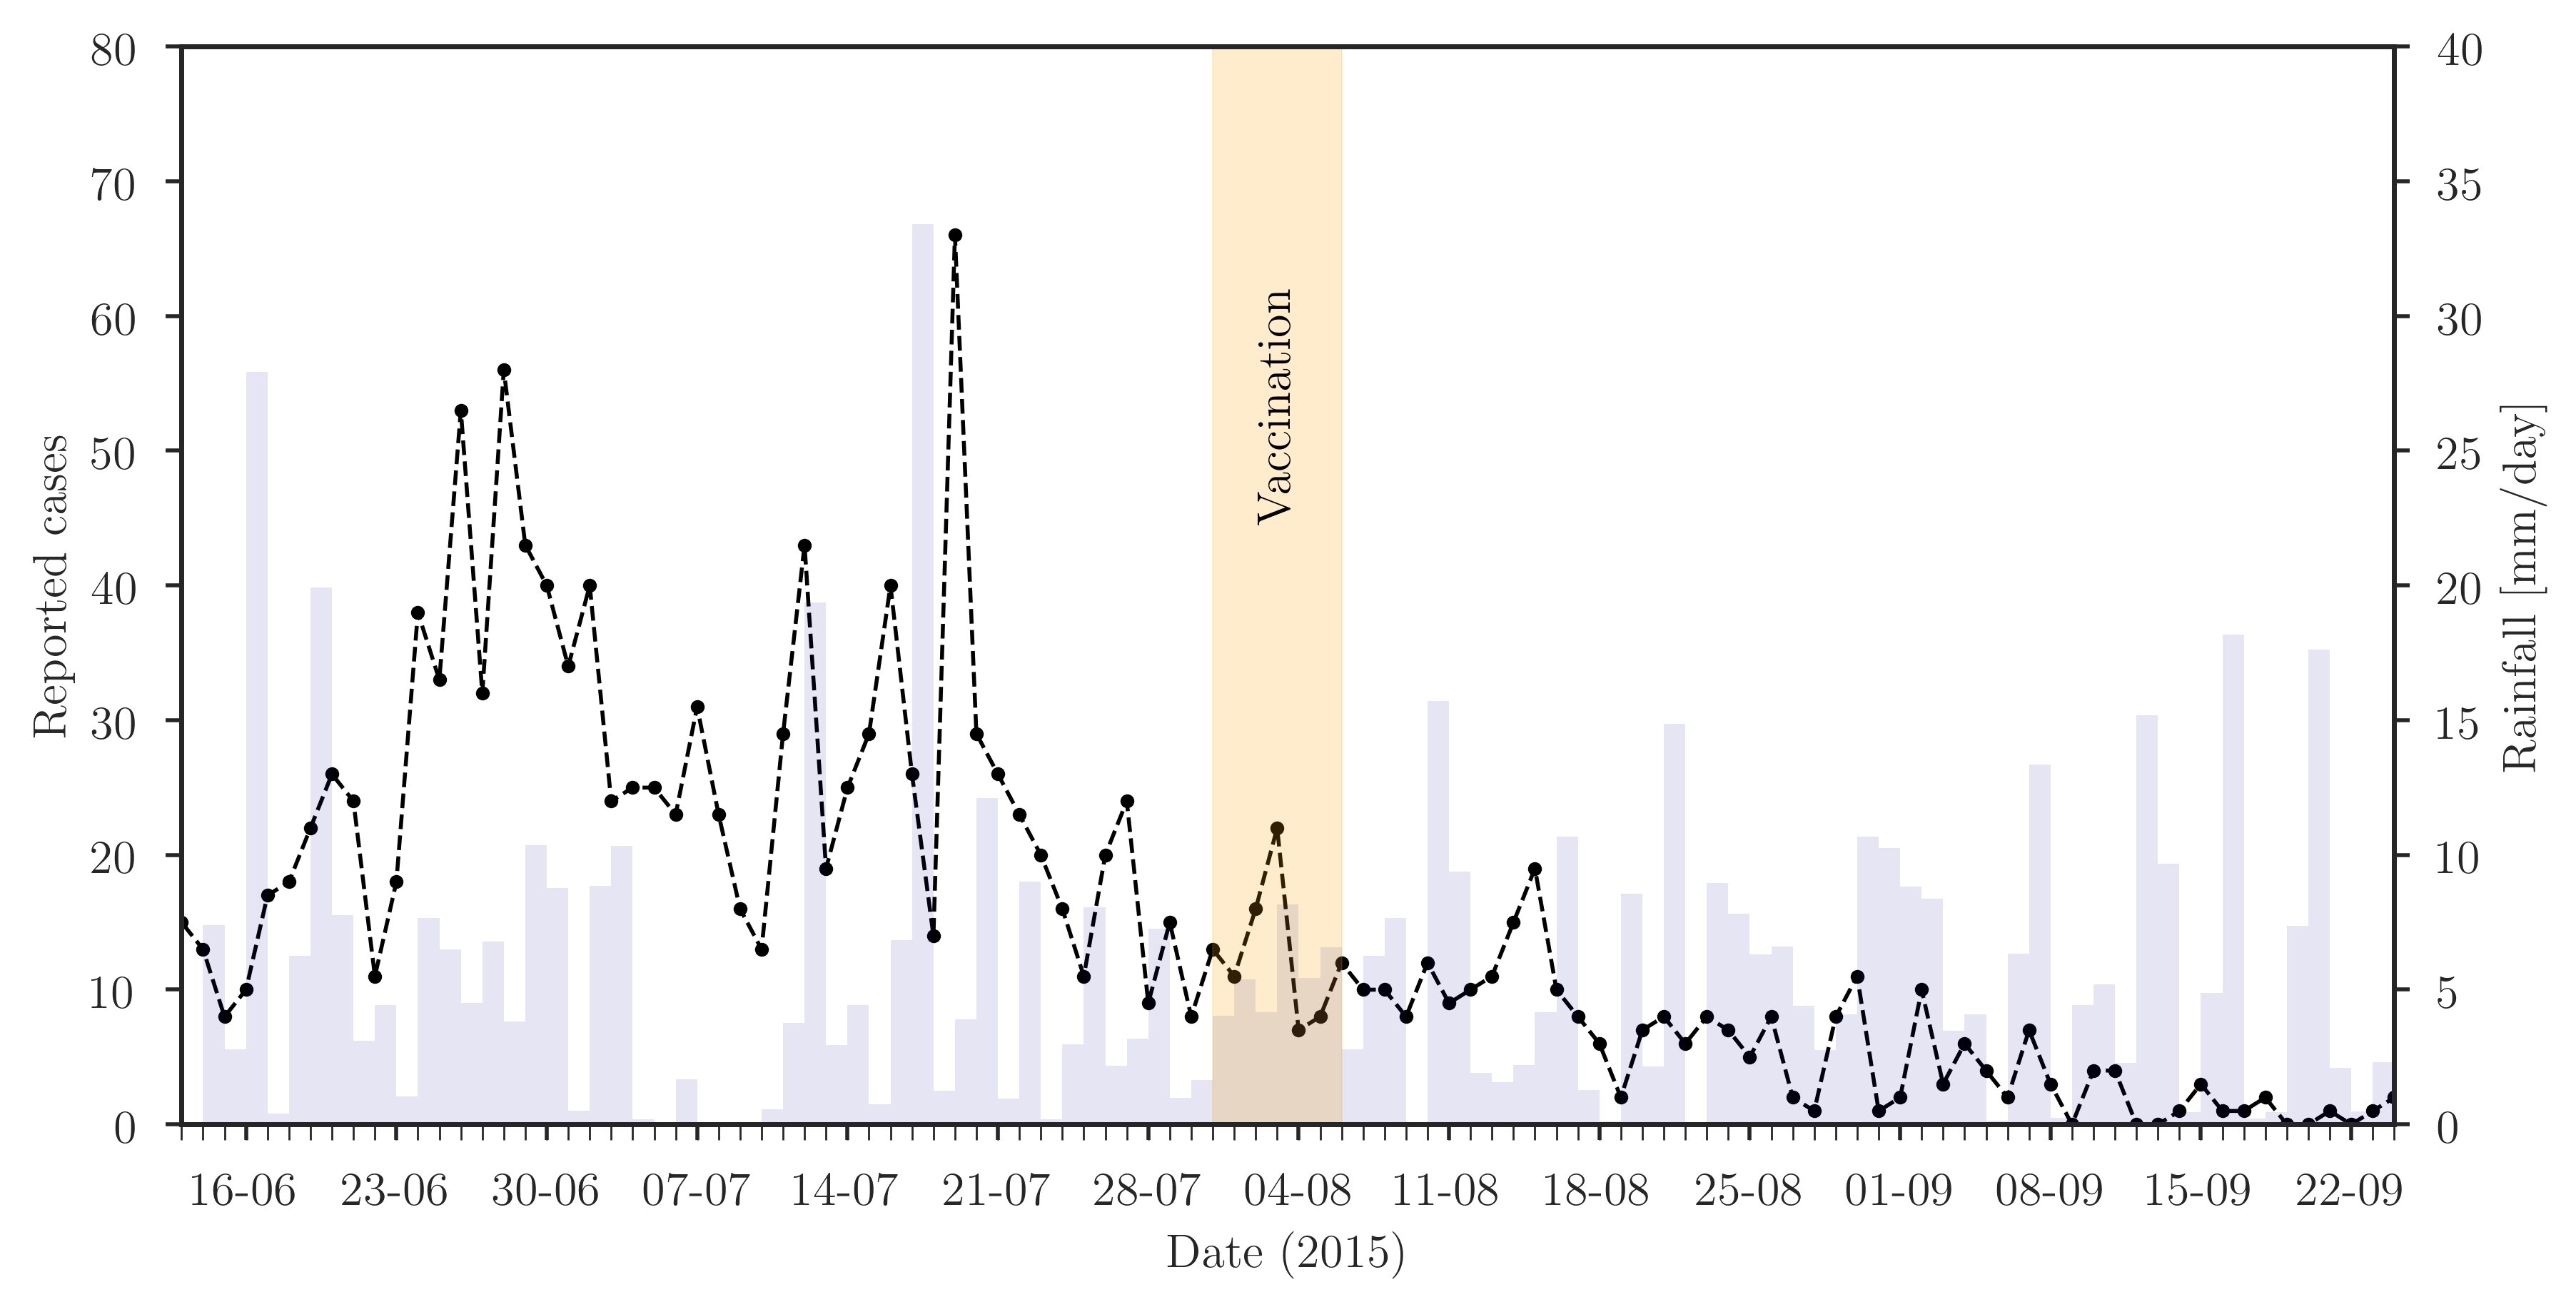
\includegraphics{fig_cholera-rainfall/Lemaitre_ACTROP_2018_42_R1_fig2.png}
  \caption[Cholera cases and precipitation during the 2015 cholera epidemic in Juba][2\baselineskip]{Reported cholera cases (dots) and precipitation (bars) during the 2015 cholera epidemic in Juba. The timing of the vaccination campaign is highlighted in yellow.}\label{fig:report}
\end{figure}
In the past years, South Sudan had been struck by several cholera outbreaks\footnote{More details on the history of cholera in South Sudan are found in: \fullcite{Sciarra:MathematicalModelingCholera:2018}}. Here the analysis focuses on the 2015 outbreak in Juba, when a particular double peak of cholera cases was associated to a strong intra-seasonal precipitation event (fig.~\ref{fig:report}). Access was to granted to epidemiological records for the 2014 and 2015 cholera epidemics that include daily cholera incident cases and hospitalization at the second-lowest administrative level (Payams), reported by the Ministry of Health of South Sudan. The cases in the 7 Payams that constitute the administrative area of Juba have been aggregated to obtain the reported time series for the county level. The population data for Juba county is taken from the South Sudan National Bureau of Statistics\cite[-4\baselineskip]{SSNBS:PopulationProjectionsSouth:2015}. Daily rainfall estimates for years 2014 and 2015 were obtained from the Climate Data Library\cite[-3.5\baselineskip][with a resolution of {0.1}$^\circ$, rainfall was averaged over the study area.]{IRI/LDEO:ClimateDataLibrary:2016}. In 2015, 167'377 OCV doses were distributed in the county of Juba during 6 days of a mass vaccination campaign started on July 31, 2015\cite[-3.2\baselineskip]{Abubakar:FirstUseGlobal:2015,Azman:EffectivenessOneDose:2016,Parker:AdaptingGlobalShortage:2017}, and are taken into account in the model.
%FFN: South Sudan has a lot of one dose
\newpage
\section{Cholera models}
\label{sec:meth}
\subsection{Generalized cholera model}
The proposed model is inspired from the model presented in the previous chapter: we have the susceptible $S$, infected $I$, and recovered $R$ compartments for individuals, with an additional variable $B$ describing the concentration of the bacteria in the environment. Previous modelling exercises had considered rainfall intensity $J(t)$ either to i) multiplicatively increase water \textit{contamination} with bacteria shed by infected  individuals\cite{Bertuzzo:ProbabilityExtinctionHaiti:2016,Pasetto:RealtimeProjectionsCholera:2017}, or ii) assumed that the rainfall multiplicatively increases the \textit{exposure} to contaminated water\cite{Eisenberg:ExaminingRainfallCholera:2013}. A generalized formulation of these cholera-forced models, wherein both formulations are nested, is proposed. It enables the systematic comparison of the effect of rainfall through these two different transmission pathways.

The model described in \textsc{Chapter~1} was designed to deal with weekly data. Here, given the daily temporal resolution at which incidence data was available for the 2015 Juba's epidemic, a compartment of exposed individuals $E$ is added to the model structure. It describe the incubation period: the lag between the time of exposure and the onset of the symptoms. Moreover, in order to account for the vaccination campaigns that were deployed in Juba in August 2015, four compartments ($V^S$, $V^E$, $V^I$, and $V^R$) are added to describe the dynamics of vaccinated individuals and their removal from the pool of susceptibles.

The proposed generalized cholera model is described in fig.~\ref{diagram}, and formulated as:
\marginnote[7\baselineskip]{
\begin{tabular}{ll}
\toprule
     symbol      & signification   \\
    \hline
$\alpha$ & cholera induced mortality\\
$\mu$ & natural mortality\\
$\sigma$ &symptomatic fraction\\
$\gamma$ & infectious period \\
$\rho$ & duration of immunity \\
$\rho_v$ & duration of vaccine protection \\
$\eta$ & vaccine efficacy \\
$\theta$ & shedding rate \\
$\mu_B$ & bacteria decay in water \\
$J(t)$ & rainfall \\
\bottomrule
\end{tabular}\\Reminder of the parameters already described in \textsc{Chapter~1} (p.\pageref{eq:I2}).}

\begingroup
\allowdisplaybreaks
\begin{eqnarray} \label{eq:fullmodel}
S(t) &=& H - I(t) - E(t) - R(t) - V^S(t) - V^E(t) - V^I(t) - V^R(t) \label{eq:S2j} \\
 \frac{dE}{dt} &=& \sigma F(t) S - (\phi + \mu +\nu) E \label{eq:E2j}\\
 \frac{dI}{dt} &=& \phi E - (\gamma + \mu + \alpha) I \label{eq:I2j}\\
 \frac{dR}{dt} &=& (1-\sigma) F(t) S + \gamma I - (\rho + \mu+\nu) R \label{eq:R2j}\\
 \frac{dB}{dt} &=& - \mu_B B +\theta\left[1 + f_{\mathcal{c}}\left(J(t)\right) \right] (I+V^I)\label{eq:B2}\\
\frac{dV^S}{dt} &=& \nu S - \mu V^S+ \rho_{v} V^R - (1-\eta) F(t) V^S \label{eq:VS2j}\\
 \frac{dV^E}{dt} &=& \nu E + \sigma (1-\eta) F(t) V^S-(\phi + \mu) V^E \label{eq:VE2}\\
 \frac{dV^I}{dt} &=&  \phi V^E -(\gamma + \alpha + \mu) V^I \label{eq:VI2j}\\
 \frac{dV^R}{dt} &=& \nu R -(\mu +\rho_{v})V^R +\gamma V^I +(1-\sigma) (1-\eta) F(t) V^S\label{eq:VR2j}\; ,
\end{eqnarray}
\endgroup
where $F(t)$ takes into account both human-to-human transmission and nonlinear water-to-human transmission:
\begin{equation}
  F(t) = \beta_B \underbrace{ \left[\frac{B}{K + B} \right] \bigg(1+f_{\mathcal{e}}\left(J(t)\right)\bigg)}_{\text{indirect transmission}} + ~\beta_{I} \underbrace{\frac{(I+V^I)}{H}}_{\text{direct transmission}}.
\label{eq:force2}
\end{equation}
 The notation is consistent with \textsc{Chapter~1} and we refer the reader to the description of the processes provided on \pageref{eq:I2}, and reminded in the margin table. In addition to tge previously decribed dynamics, exposed individuals become symptomatic infected at a rate $\phi$, which corresponds to an average incubation period of $1/\phi\approx$ 1.5 days\cite{Azman:IncubationPeriodCholera:2013}. As few reliable data on changes in Juba's population are available for the years of interest, the total population $H$, is assumed to be constant, as in \eqref{eq:S2j}. 
 
Moreover, the effect of rainfall is more precisely described. Functions $f_{\mathcal{c}}\left(J(t)\right)$ and $f_{\mathcal{e}}\left(J(t)\right)$ account for the rainfall effect respectively by increasing the bacteria contamination in the water reservoir or directly through amplifying the exposure in the force of infection.
\begin{figure}
  \centering
  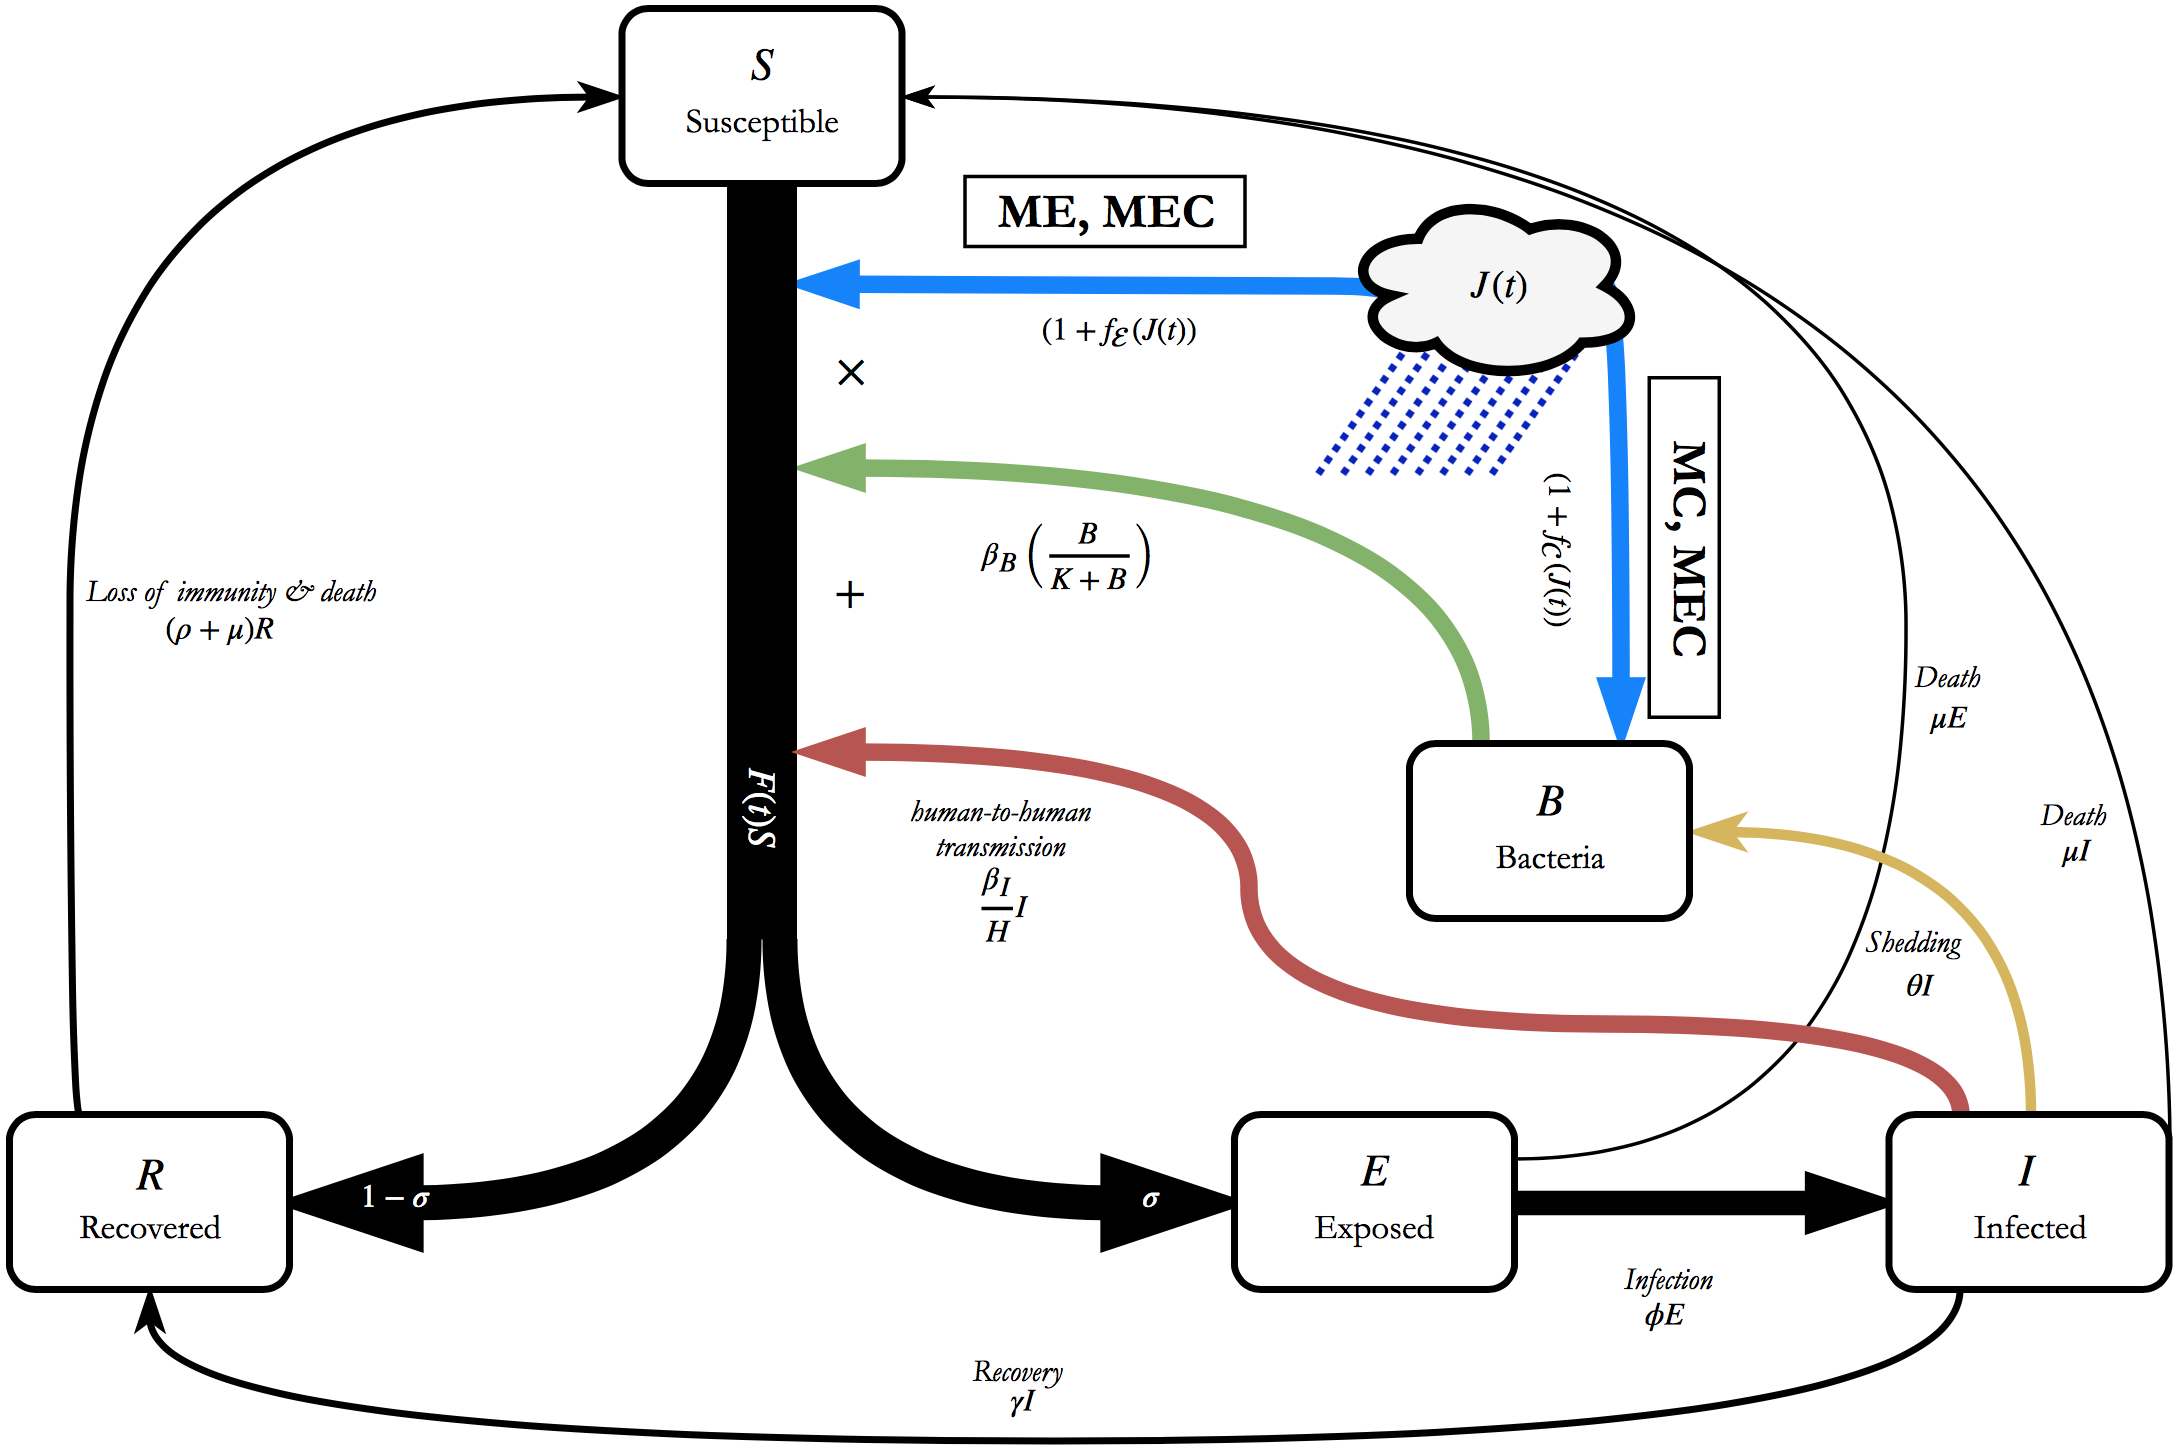
\includegraphics{fig_cholera-rainfall/Lemaitre_ACTROP_2018_42_R1_fig1.png}
  \caption[Transition diagram for the competing cholera models]{Transition diagram for the different cholera models considered, with the different variations \textsc{me}, \textsc{mr}, and \textsc{mec} indicated.}
  \label{diagram}
\end{figure}
With the objective of assessing the importance of rainfall on cholera transmission, a generalization of the linear relation found in the litterature\footnote{Specifically the reference exposure \parencite{Eisenberg:ExaminingRainfallCholera:2013} and contamination \parencite{Rinaldo:Reassessment20102011:2012} models.} is proposed, by using a nonlinear function form for  $f_{\mathcal{c,e}}\left(J(t)\right)$:
\begin{equation}
    f_{\mathcal{c,e}}\left(J(t)\right)=\lambda_{\mathcal{c,e}} \left(\frac{J(t)}{\max_t J(t)}\right)^{\alpha_{\mathcal{c,e}}}
    \label{eq:nonlinear_rain}
\end{equation}
\begin{marginfigure}
	\centering
	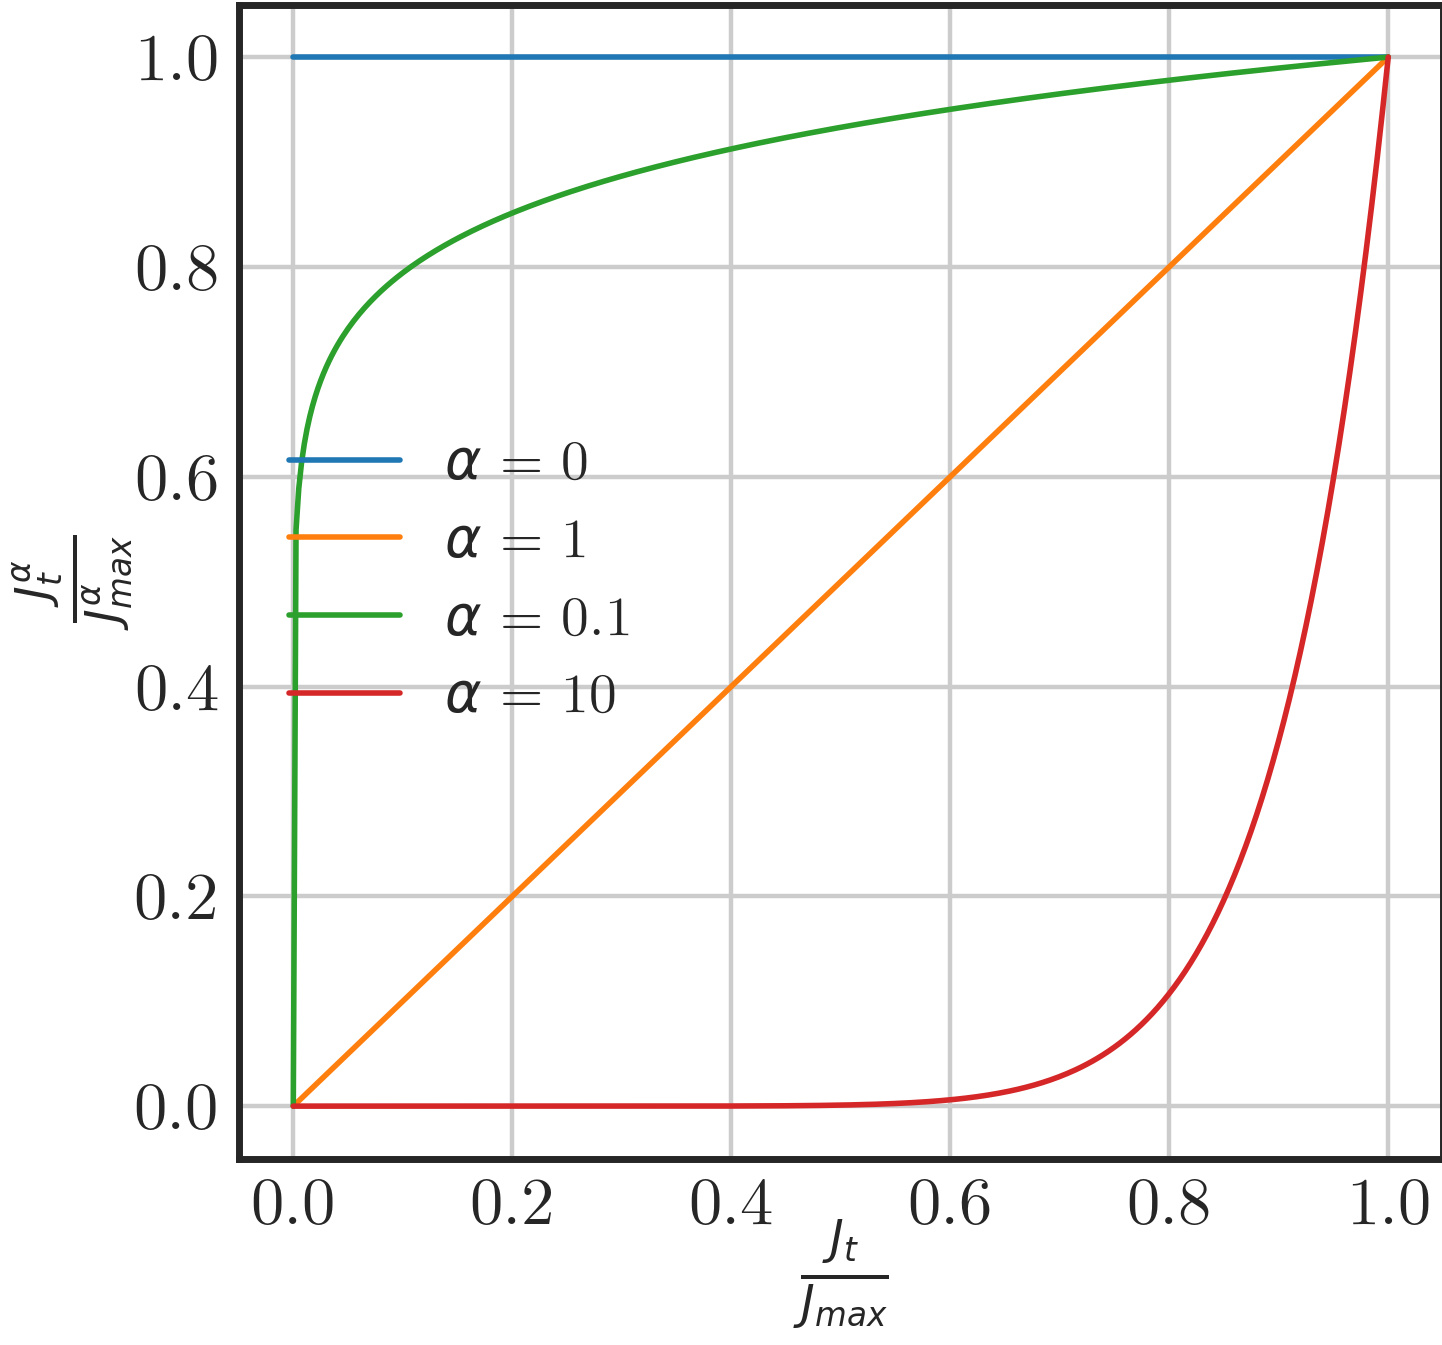
\includegraphics{fig_cholera-rainfall/alpha.png}
	\margincaption[Non-linear rainfall effect on transmission]{$\left(\frac{J_t}{J_{max}}\right)^\alpha$ for different values of $\alpha$. For $\alpha = 1$, the linear model described in previous works is obtained, and larger $\alpha$ corresponds to an increased relative importance of heavy rainfall events.}
	\label{fig:alpha}
\end{marginfigure}
where the subscripts $_\mathcal{c,e}$ respectively denote the effect of rainfall on exposure and contamination, $\max_t J(t)$ is the maximum recorded rainfall intensity during the epidemic, and the $\alpha_{\mathcal{c,e}}\ge0$ controls for the relative importance of different rainfall intensities in their effect on the force of infection. Indeed, since the ratio $\frac{J(t)}{\max_t J(t)} \in [0,1]$, for $\alpha_{\mathcal{c,e}} \gg 1$ the ratio will tend to $0$ for all small precipitation events, leaving only the effect of the strongest events, whereas for $\alpha_{\mathcal{c,e}} < 1$ all precipitation events will be assigned a similar weight in the force of infection (fig. \ref{fig:alpha}). The formulations found in litterature are recovered by setting $\alpha_{\mathcal{c,e}} = 1$. The flexibility allowed by eqn.~\eqref{eq:nonlinear_rain} allows to discriminate between rainfall effects along a continuum from acting on disease transmission regardless of intensity to a threshold-like effect for the largest events which could be associated to severe flooding causing damages to the city's water and sanitary system, for instance leading to sewer overflow.

\subsection{Competing transmission models}
The relevance of the two rainfall-driven transmission pathways is assessed here by comparing the following models:
\begin{itemize}
 \item \textsc{mn} SIRB model without rainfall: $\lambda_{\mathcal{c}} = \lambda_{\mathcal{e}} = 0$, $\beta_{I} = 0$, as the null hypothesis for the importance of rainfall.
  \item \textsc{mc} SIRB model where for rainfall enhances the \textit{contamination} of the water reservoir: $\lambda_{\mathcal{e}} = 0$, $\beta_{I} = 0$. 
  \item \textsc{me} SIRB model where rainfall increases the \textit{exposure} to bacteria: $\lambda_{\mathcal{c}} = 0$, $\beta_{I} = 0$. 
  \item \textsc{mec} SIRB model combining both approaches \textsc{mc} and \textsc{me} ($\beta_{I} = 0$). Both ways of accounting rainfall play a role simultaneously.
\end{itemize}
\marginnote[-8\baselineskip]{\textsc{me} models uses a similar transmission pathway as in \textcite{Eisenberg:ExaminingRainfallCholera:2013}, whereas \textsc{mc} models were described in \textcite{Rinaldo:Reassessment20102011:2012}. These models were adapted to the generalized configuration, \eg in eqn.~\eqref{eq:force2} precipitation enters in the term $\left(1+f_E \left(J(t)\right)\right)$ which entails water-to-human transmission also when $J(t)=0$, unlike the published version. The steps take to adapt these models are shown in the postprint supplementary, section S.1.}
\begin{table}[h!]
\centering
\begin{tabular}{lccccc}
\toprule
     Model       & $\lambda_{\mathcal{c}}$ & $\alpha_\mathcal{c}$ & $\lambda_{\mathcal{e}}$ & $\alpha_\mathcal{e}$ & $\beta_I$   \\
    \hline
    \textsc{mn} &       --    &    --   &       --      &       --      &  -- \\
    \textsc{mnh} &     --      &   --    &    --         &        --     &   $\times$ \\
    \textsc{mc} &      $\times$  &  $\times$  &     --        &       --      &  -- \\
    \textsc{me} &         --  &   --    &      $\times$    &   $\times$        & --  \\
    \textsc{mch}&      $\times$  &  $\times$  &      --       &     --        &$\times$ \\
    \textsc{meh}&        --   &  --     &      $\times$    &   $\times$        &$\times$ \\
    \textsc{mec}&      $\times$ &  $\times$  &      $\times$    &    $\times$      & --\\
    \textsc{mech}&      $\times$ &  $\times$  &      $\times$    &    $\times$       &   $\times$ \\
\bottomrule
\end{tabular}
\caption[Parameters considered in the eight compared models]{Parameters considered in the eight compared models.  $\lambda$ and $\alpha$ characterize the functional forms considering the precipitation eqn.~\eqref{eq:nonlinear_rain}. $\beta_I$ is the exposure for human-to-human transmission. A dash -- indicate that the parameter is set to zero, whereas a cross $\times$  indicate that the parameter is used.}
\label{tab:models}
\end{table}

 For each model is explored the possibility of adding explicitly direct, human-to-human transmission ($\beta_{I} > 0$), which is indicated with an \textsc{H} at the end of the model name: \textsc{mnh}, \textsc{mch}, \textsc{meh}, and \textsc{mech}. The different parameters associated with the considered models are summarized in tab.~\ref{tab:models}.

 The eight models are compared on the basis of their ability to match the time series of daily reported cases during the cholera epidemic in Juba of 2015. In the postprint, tab. S.1 summarizes which parameters are calibrated for each model and their prior distribution. The degrees of freedom of the models, $n_p$, vary from $n_p=7$ for \textsc{mn} to $n_p=12$ for \textsc{mech}. Given the low number of daily reported cases and their ensuing variability, a stochastic equivalent is also implemented\footnote[][-8\baselineskip]{The sole difference in formulation is the introduction of overdispersion in the infection process. The force of infection is multiplied by a time-continuous white noise process, as detailled in the eqns. \eqref{eqn:sta}--\eqref{eqn:stb}.} of the deterministic ODE system, eqns. \eqref{eq:fullmodel}-\eqref{eq:VR2j}, formulated as a continuous time partially observed Markov process model, accounting for both demographic and disease transmission stochasticities\cite{Breto:TimeSeriesAnalysis:2009}. The formulation of the stochastic model is left in the \textsc{Appendix}, eqn. \eqref{eq:stochsys} on p. \pageref{eq:stochsys}.

\subsection{Models calibration}
\marginnote{For details about fixed and calibrated parameters, along with prior and posterior distributions, the reader is referred to the supplemental information of \fullcite{Lemaitre:RainfallDriverEpidemic:2019}.}
\paragraph{Initial conditions} The past history of cholera epidemics in South Sudan, and particularly in Juba, plays an important role in the determination of the size of susceptible and recovered compartments at the beginning of the 2015 epidemic. These two compartments are also largely impacted by the rate of immunity loss $\rho$ of the recovered individuals, and by the probability of asymptomatic infection $1-\sigma$\footnote[][2\baselineskip]{values in literature range between $\sigma=0.5$, meaning one asymptomatic per each symptomatic infected, to less than $\sigma=0.01$, corresponding to more than 99 asymptomatic infected per each symptomatic infected \parencite{Fung:CholeraTransmissionDynamic:2014}.}. The initial conditions must therefore be estimated for each parameter set considered during calibration.

 
 To take into account the uncertainty associated with the immunity landscape of Juba, the initial number of recovered individuals in April 2014 is calibrated for each model. Then, the detailed daily data of suspected cases during 2014 is used to estimate the associated number of recovered individuals at the start of the 2015 epidemic. Suspected cases in 2014 are scaled to the reporting fraction and  undergo an exponential decay with average time of immunity loss $1/\rho$\footnote{Something similar has been done in \parencite{Pasetto:RealtimeProjectionsCholera:2017}.}. Simulations are then initialized on June 5, 2015 considering two exposed individuals, two infected, and the associated steady-state bacteria concentration. 
 
\paragraph{Calibration} Calibration of the deterministic model is performed using a Markov Chain Monte Carlo based algorithm\footnote{Differential Evolution Adaptive Metropolis, \textsc{dream}: \parencite{Vrugt:MarkovChainMonte:2016}, which was developed to explore high-dimensional parameter spaces. Given the parameters' prior distribution, \textsc{dream} searches and selects new samples in the posterior distribution by using multiple \textsc{mcmc} chains that run in parallel and that jointly contribute to the computation of the proposal parameter samples. \textsc{Mcmc} chains  converge toward the posterior probability distribution based on the log-likelihood function of the data given the model output.} , which draws samples from the posterior distribution of the parameters.
Inference on the stochastic model is performed using a frequentist iterated filtering algorithm\footnote{MIF, an algorithm proposed by \parencite{Ionides:InferenceDynamicLatent:2015}, which is a frequentist-based approach for identifying the maximum likelihood estimation. It has proved successful even for a range of complex models of cholera dynamics \parencite{King:InapparentInfectionsCholera:2008,Baracchini:SeasonalityCholeraDynamics:2017}. The MIF2 algorithm, which employs iterated Bayes maps, is implemented in the R package \texttt{pomp} \parencite{King:StatisticalInferencePartially:2015}. %For this exercise, it is configured using 120 initial parameter vectors for each model, built using Sobol sequences over the parameter bounds.
}. Both model were fit against the daily reported cases accounting for over- or under- reporting, and assuming a Poisson likelyhood\shortcite{Camacho:CholeraEpidemicYemen:2018}. Each datapoint at reporting date $t_i$,  $y_{t_i}$, is assumed to belong to a Poisson distribution centered on the modeled incidence $C_{t_i}$\footnote{$C_{t_i}$ is computed as in  eqn. \eqref{eq:C}, but for the $E \rightarrow I$ transition. For the deterministic model: $ C_{t_i} = \int_{t_i}^{t_{i+1}} \phi \left(E(t) + V^E(t)\right) dt$. For the stochastic model the reporting process is described in eqn. \eqref{eq:stochrep}.
% $ C_{t_i} = [N_{EI}(t_{i+1}) - N_{EI}(t_i)] + [N_{V^EV^I}(t_{i+1}) - N_{V^EV^I}(t_i)] $, where $N_{AB}$ denotes the stochastic counting process of transitions between classes $A$ and $B$ .
} and its associated parameter vector $\boldsymbol{\theta}$ altered by the reporting rate $\epsilon$, as:
\begin{equation}
 y_{t_i}  \sim \text{Poisson}\left(\epsilon \,C_{t_i}(\boldsymbol{\theta})\right), \; \epsilon > 0,
 \label{eq:obs}
\end{equation}
 Models were then compared using the Bayesian Information criterion (BIC), Bayes factors, and the likelihood ratio test for the nested models.
 
 
\section{Results}

\subsection{Model selection of the rainfall effects on cholera transmission}
The summary statistics of the deterministic and stochastic models considered in the study are given in tab.~\ref{tab:stats}. Overall, the stochastic models outperform their deterministic counterparts for all model structures by $\approx 40$ log-likelihood units. Both model types agree in the significance of rainfall in explaining the time series of daily reported cases, in particular through the increased exposure pathway, although the specific ordering of the models differs between model types. The BFs for the deterministic models suggest a strong support for model \textsc{mec}, followed by model \textsc{me} ($BF^{-1}_{ME,MEH} = 0.16$), with very little support for all other models ($BF^{-1}_{\boldsymbol{\cdot},MEH}< 10^{-2}$ for all other models than ME). For the stochastic model, the BFs estimated with the BIC suggest the strongest support for model \textsc{me}, with the basic SIRB model coming in second with 5 times less evidence ($BF^{-1}_{MN,ME} \approx 0.15$). 
\begin{table}[h!]
\centering
\small
\begin{tabular}{lcccccccc}
  \toprule
  & \multicolumn{4}{c}{Deterministic} & \multicolumn{4}{c}{Stochastic} \\
    \cmidrule(rl){2-5}\cmidrule(rl){6-9}
  Model & $n$ & $\hat{\ell}$ & BIC & ${BF}^{-1}$ & $n$ & \makecell{$\hat{\ell}$ \vspace{-.1cm} \\ \scriptsize{(s.e.)}}  & BIC  & $BF^{-1}$ \\ 
  \cmidrule(rl){2-5}\cmidrule(rl){6-9}
  \textsc{mn} &   7 & -368.62 & 770.27 & 3.1E-05 &   8 & \makecell{-326.45 \vspace{-.1cm} \\ \scriptsize{(0.105)}} & 690.65 & 1.5E-01 \\ 
   \textsc{mnh} &   8 & -368.95 & 775.64 & 1.1E-09 &   9 & \makecell{-327.52\vspace{-.1cm} \\ \scriptsize{(0.052)}} & 697.51 & 4.7E-03 \\ 
   \textsc{mc} &   9 & -358.32 & 759.11 & 5.5E-03 &  10 & \makecell{-323.50\vspace{-.1cm} \\ \scriptsize{(0.037)}} & 696.01 & 2.5E-02 \\ 
   \textsc{mch} &  10 & -359.06 & 765.30 & 1.7E-04 &  11 & \makecell{-324.89\vspace{-.1cm} \\ \scriptsize{(0.041)}} & 701.68 & 5.9E-04 \\ 
   \textsc{me} &   9 & -356.96 & \textsc{756.40} & 1.6E-01 &  10 & \makecell{\textsc{-319.81}\vspace{-.1cm} \\ \scriptsize{(0.035)}} & \textsc{687.38} & \textsc{1} \\ 
   \textsc{meh} &  10 & -358.06 & 763.30 & 6.3E-04 &  11 & \makecell{-320.64\vspace{-.1cm} \\ \scriptsize{(0.030)}} & 693.18 & 4.1E-02 \\ 
   \textsc{mec} &  11 & \textsc{-356.87} & 765.64 & \textsc{1} &  12 & \makecell{-320.17\vspace{-.1cm} \\ \scriptsize{(0.031)}} & 696.96 & 6.2E-03 \\ 
   \textsc{mech} &  12 & -357.55 & 771.73 & 2.4E-06 &  13 & \makecell{-320.38\vspace{-.1cm} \\ \scriptsize{(0.024)}} & 702.09 & 4.8E-04 \\ 
   \bottomrule
\end{tabular}
\caption[Model comparison statistics]{Model comparison statistics. For each model is reported its number of parameters $n$, the associated estimated log-likelihood $\hat{\ell}$ (and its Monte Carlo standard error for the stochastic model), and the inverse of the Bayes Factor ($BF^{-1}$) with respect to the model with the largest evidence. The BFs for the deterministic models were computed directly from the parameters posteriors, whereas for the stochastic models they were estimated with the Bayesian Information Criterion (BIC) as $BF_{i} \approx e^{\frac{1}{2} \left( BIC_i - BIC_{min}\right)}$. The BIC for the deterministic models was computed using the maximum log-likelihood value visited with the MCMC algorithm across chains.}\label{tab:stats}
\end{table}
When considering only the BIC, model \textsc{me} ranks first for both the deterministic and the stochastic formulations. Interestingly, all models that include human-to-human transmission present smaller or equal log-likelihoods than their counterparts with only the bacteria compartment, which suggests that the data does not support both environmental and human-to-human transmission within the set of the models considered here.

The results of the nested LR-tests confirm the statistical significance of including rainfall in the cholera transmission models, with the effect on exposure better supported by the data in both model types than the effect on contamination. In the deterministic case, the extension of the basic SIRB (model \textsc{mn}) with rainfall effects were significant for all direct comparisons (fig.~\ref{fig:lltests},\textsc{a}). The addition of human-to-human transmission was not significant mostly due to the above-mentioned lower estimate of the log-likelihood in these models. When considering only a single effect of rainfall (either increasing exposure or contamination), \textsc{me} outperforms \textsc{mc} in terms of likelihood for the same number of parameters. Interestingly, the inclusion of rainfall-induced contamination in model \textsc{me} is rejected due to the very limited increase of the estimated log-likelihood of \textsc{mec}, in contrast with the BFs favouring the latter. Model \textsc{me} is thus the one retained by the LR-tests in the deterministic set of models. In the case of the stochastic models, the LR-tests also highlight the importance of the effect of rainfall on exposure rather than on contamination (fig.~\ref{fig:lltests},\textsc{b}). In fact, the much stronger performance of \textsc{mn} in comparison with its deterministic counterpart relative to all other model structures imposes a stronger condition for retaining additional transmission processes. Indeed, both models \textsc{mc} and \textsc{mch} were rejected when compared to \textsc{mn}, thus only models with rainfall-driven exposure were retained. As in the deterministic case, model \textsc{me} is the one finally retained due to the lack of significance of the inclusion of additional transmission processes. Note that the conclusion based on the LR-tests for the deterministic models should be taken with caution because the \textsc{mcmc} algorithm used for calibration does not directly aim at maximizing the likelihood, but rather at sampling from the posterior distribution of the parameters given the data and the model. Moreover, the best likelihood visited by the chains when sampling the posteriors that are used in the LR-tests is not a formal estimate of the models' likelihood. However, the fact that the LR-tests applied to both model types agree with the selection of \textsc{me} supports their use in both cases.
\begin{figure*}
    \centering
    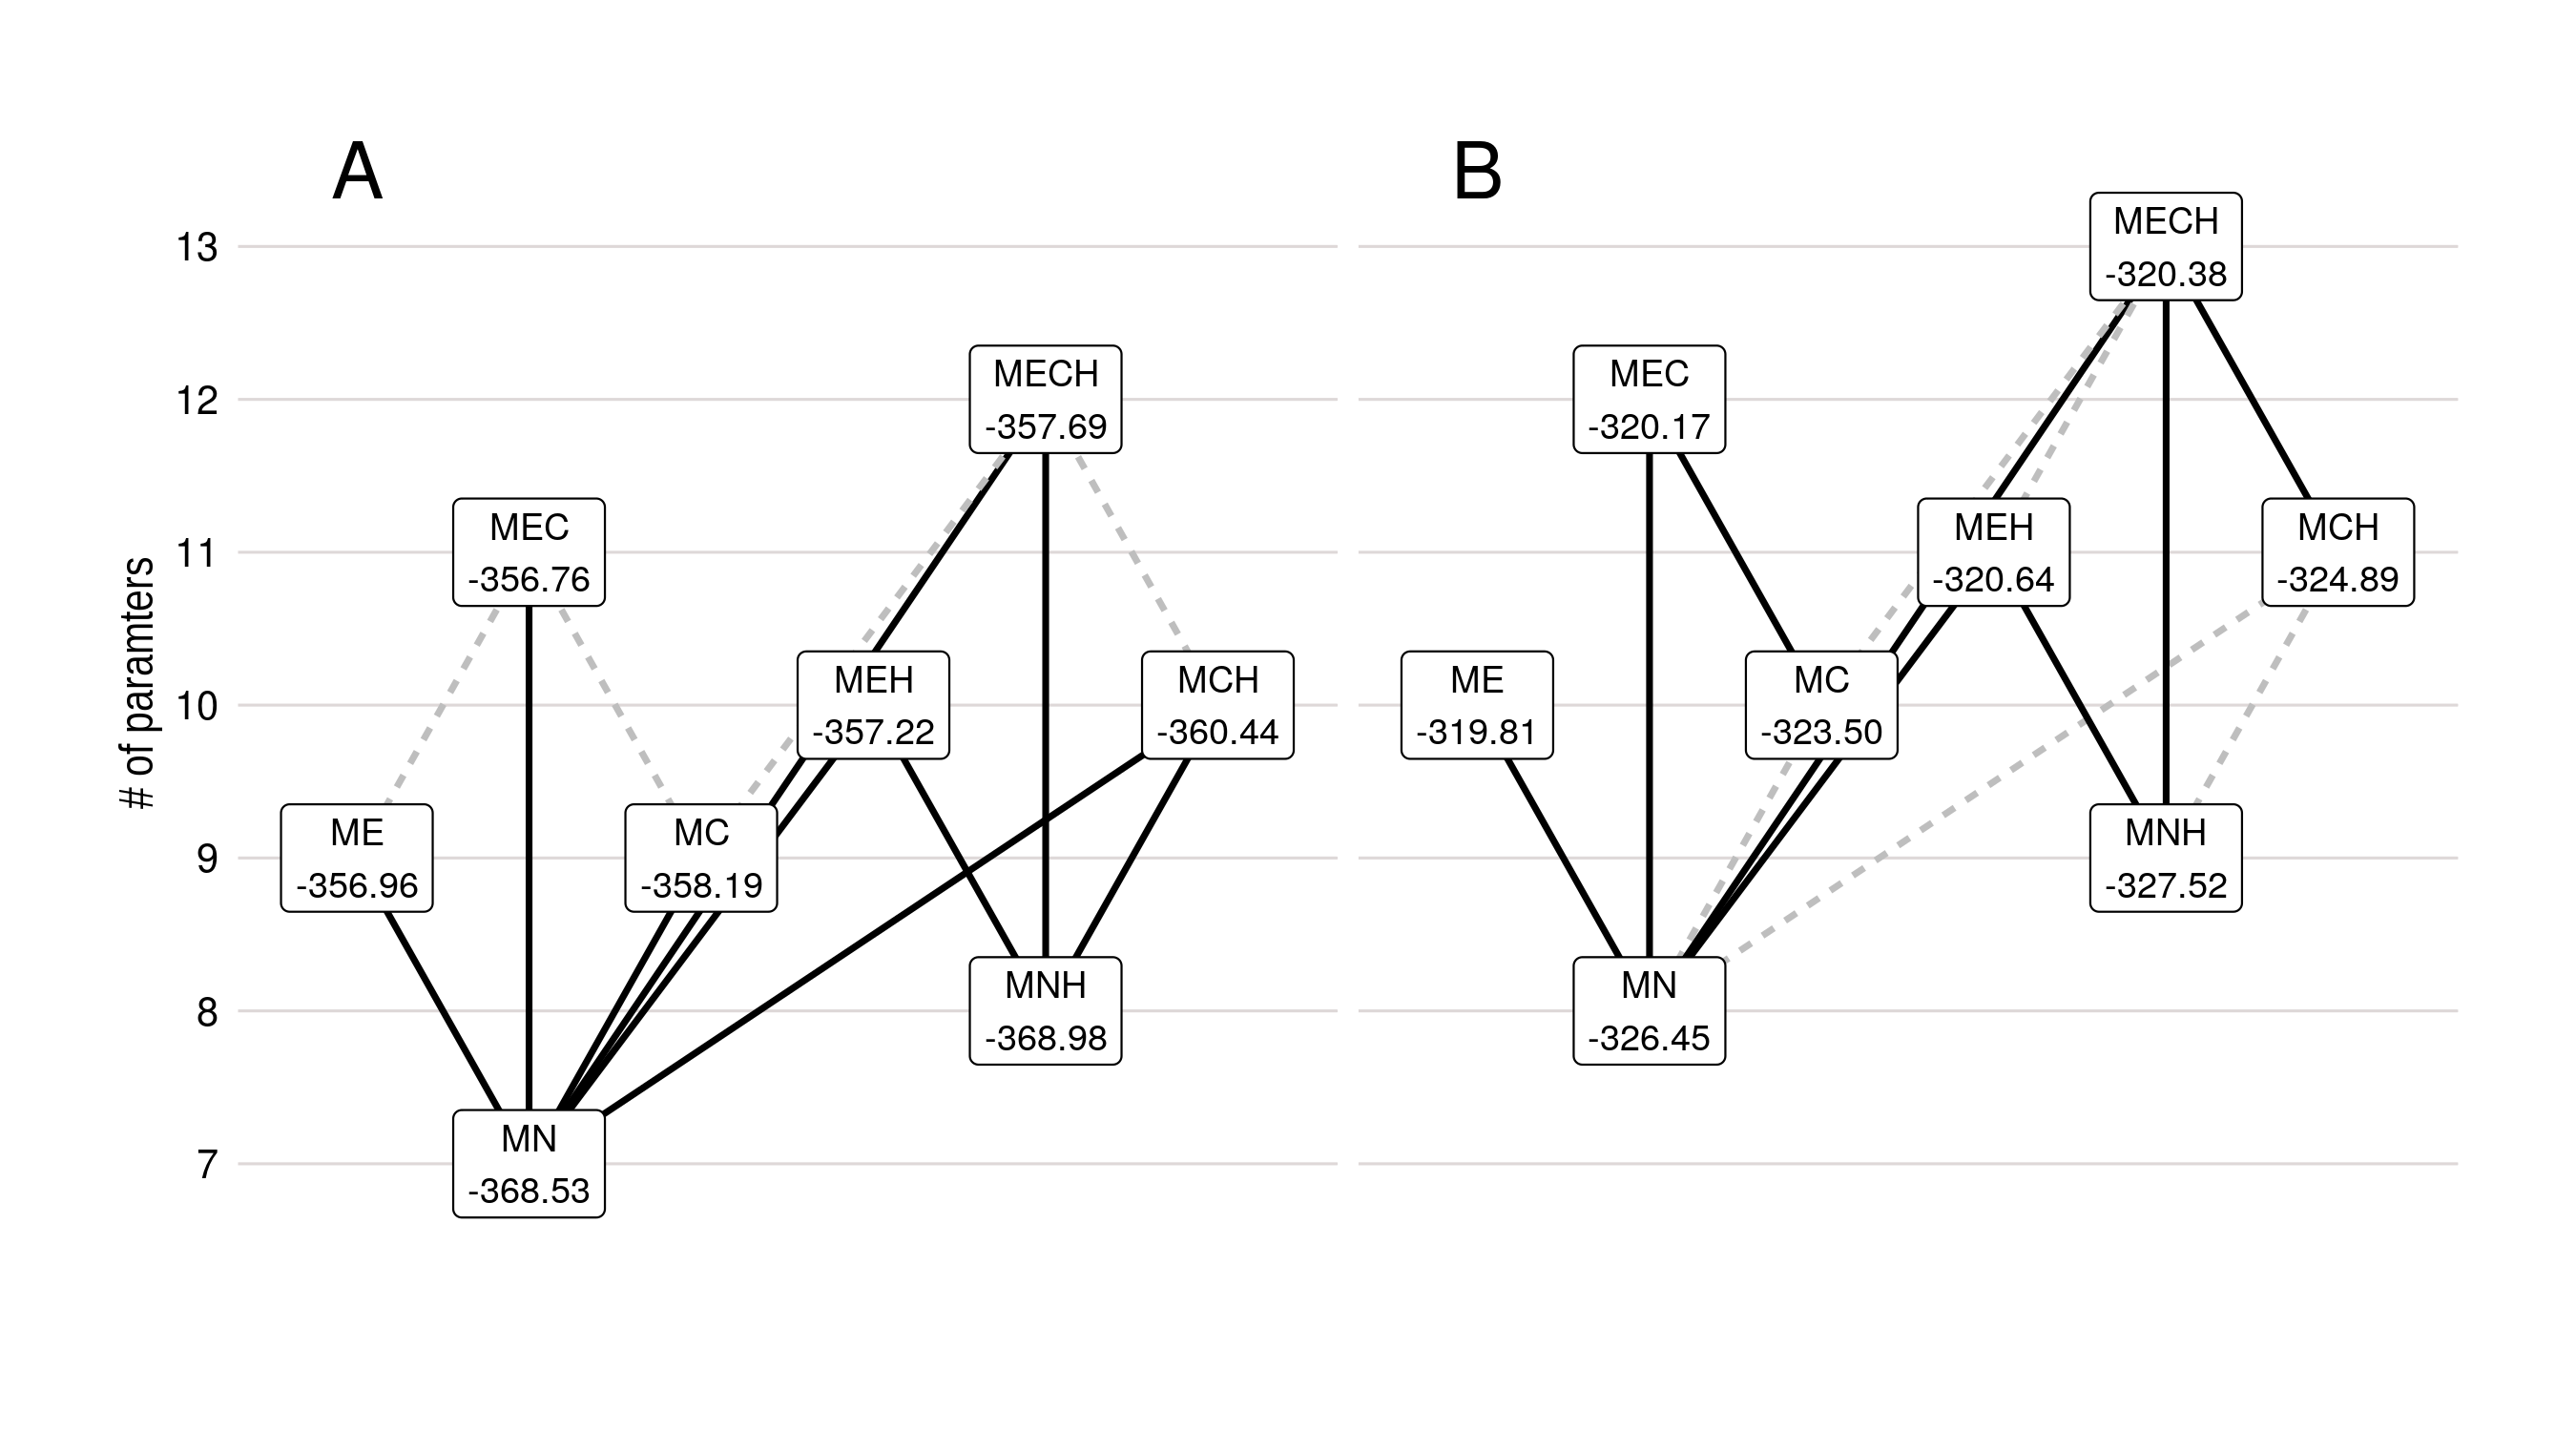
\includegraphics[width = \textwidth, trim = 11mm 19mm 10mm 12mm, clip]{fig_cholera-rainfall/Lemaitre_ACTROP_2018_42_R1_fig3.png}
    \caption[Likelihood ratio tests of model nesting]{Likelihood ratio tests of model nesting. The LL-tests were computed for each nested pair of models $\{\mathcal{M}_0, \mathcal{M}_1\}$, with parameter vectors $\boldsymbol{\theta}^0,\boldsymbol{\theta}^1$, for which at least on of the parameters that is not null is $\boldsymbol{\theta}^1$ is equal to $0$ in $\boldsymbol{\theta}^0$. Each model is labeled with its associated estimated maximum log-likelihood value, $\hat{\ell}$, for the deterministic (A) and the stochastic (B) models, and linked based on whether the likelihood ratio is significantly (full black lines) or not (dashed gray lines) at the 5\% level. The absence of lines indicates a lower $\hat{\ell}$ for the more complex model.} 
    \label{fig:lltests}
\end{figure*}


Both statistical methods for model comparison therefore agree about the importance of the effect of intra-seasonal rainfall on the exposure to transmission during the 2015 cholera epidemic in Juba. For the deterministic type of models the BFs suggest a stronger support for model \textsc{mec}, and the LR-tests for \textsc{me}, whereas for the stochastic models both the BIC-based estimates of BFs and the LR-tests favor \textsc{me}. 

\subsection{Intra-seasonal rainfall events and the 2015 Juba epidemic}

The comparison between the estimated output cases computed by the basic SIRB model (\textsc{mn}) and the most significant rainfall-based processes (\textsc{mec} and \textsc{me} for the deterministic and stochastic types, respectively) highlight the importance of rainfall in retrieving the second epidemiological peak (fig.~\ref{fig:sim}). Both deterministic and stochastic models fit well the general trend of the data, but they clearly underestimate the large number of reported cases on the 19th of July (65 cases). Instead, the more complex models \textsc{me} and \textsc{mec} follow the SIRB dynamics and then are forced by the precipitation occurred in the 18th of July (33 mm/d)  toward the epidemiological peak. 
%

Model calibration results suggest that precipitations with smaller intensities did not have a strong impact on cholera transmission during the 2015 epidemic in Juba. Indeed, the exponents $\alpha_{\mathcal{c}}$ and $\alpha_{\mathcal{e}}$ were found to be systematically larger than 1. %  (as shown by posteriors of the deterministic models in fig. S.2 and the Monte Carlo confidence intervals for the stochastic \textsc{me} in fig. S.4 of the SI) --> appendix or not ? DECISION
  Thus, in the considered epidemic, the nonlinear function used to account for rainfall in the model, eqn.~\eqref{eq:nonlinear_rain}, helps isolating the contribution of the largest rainfall.

The best measures of fit computed for the stochastic \textsc{me} (see tab.~\ref{tab:stats}) are thus explained by a larger sensitivity to precipitation, which causes the match between the mean of the simulated cases and the data during the second peak.

\begin{figure}[ht]
    \centering
    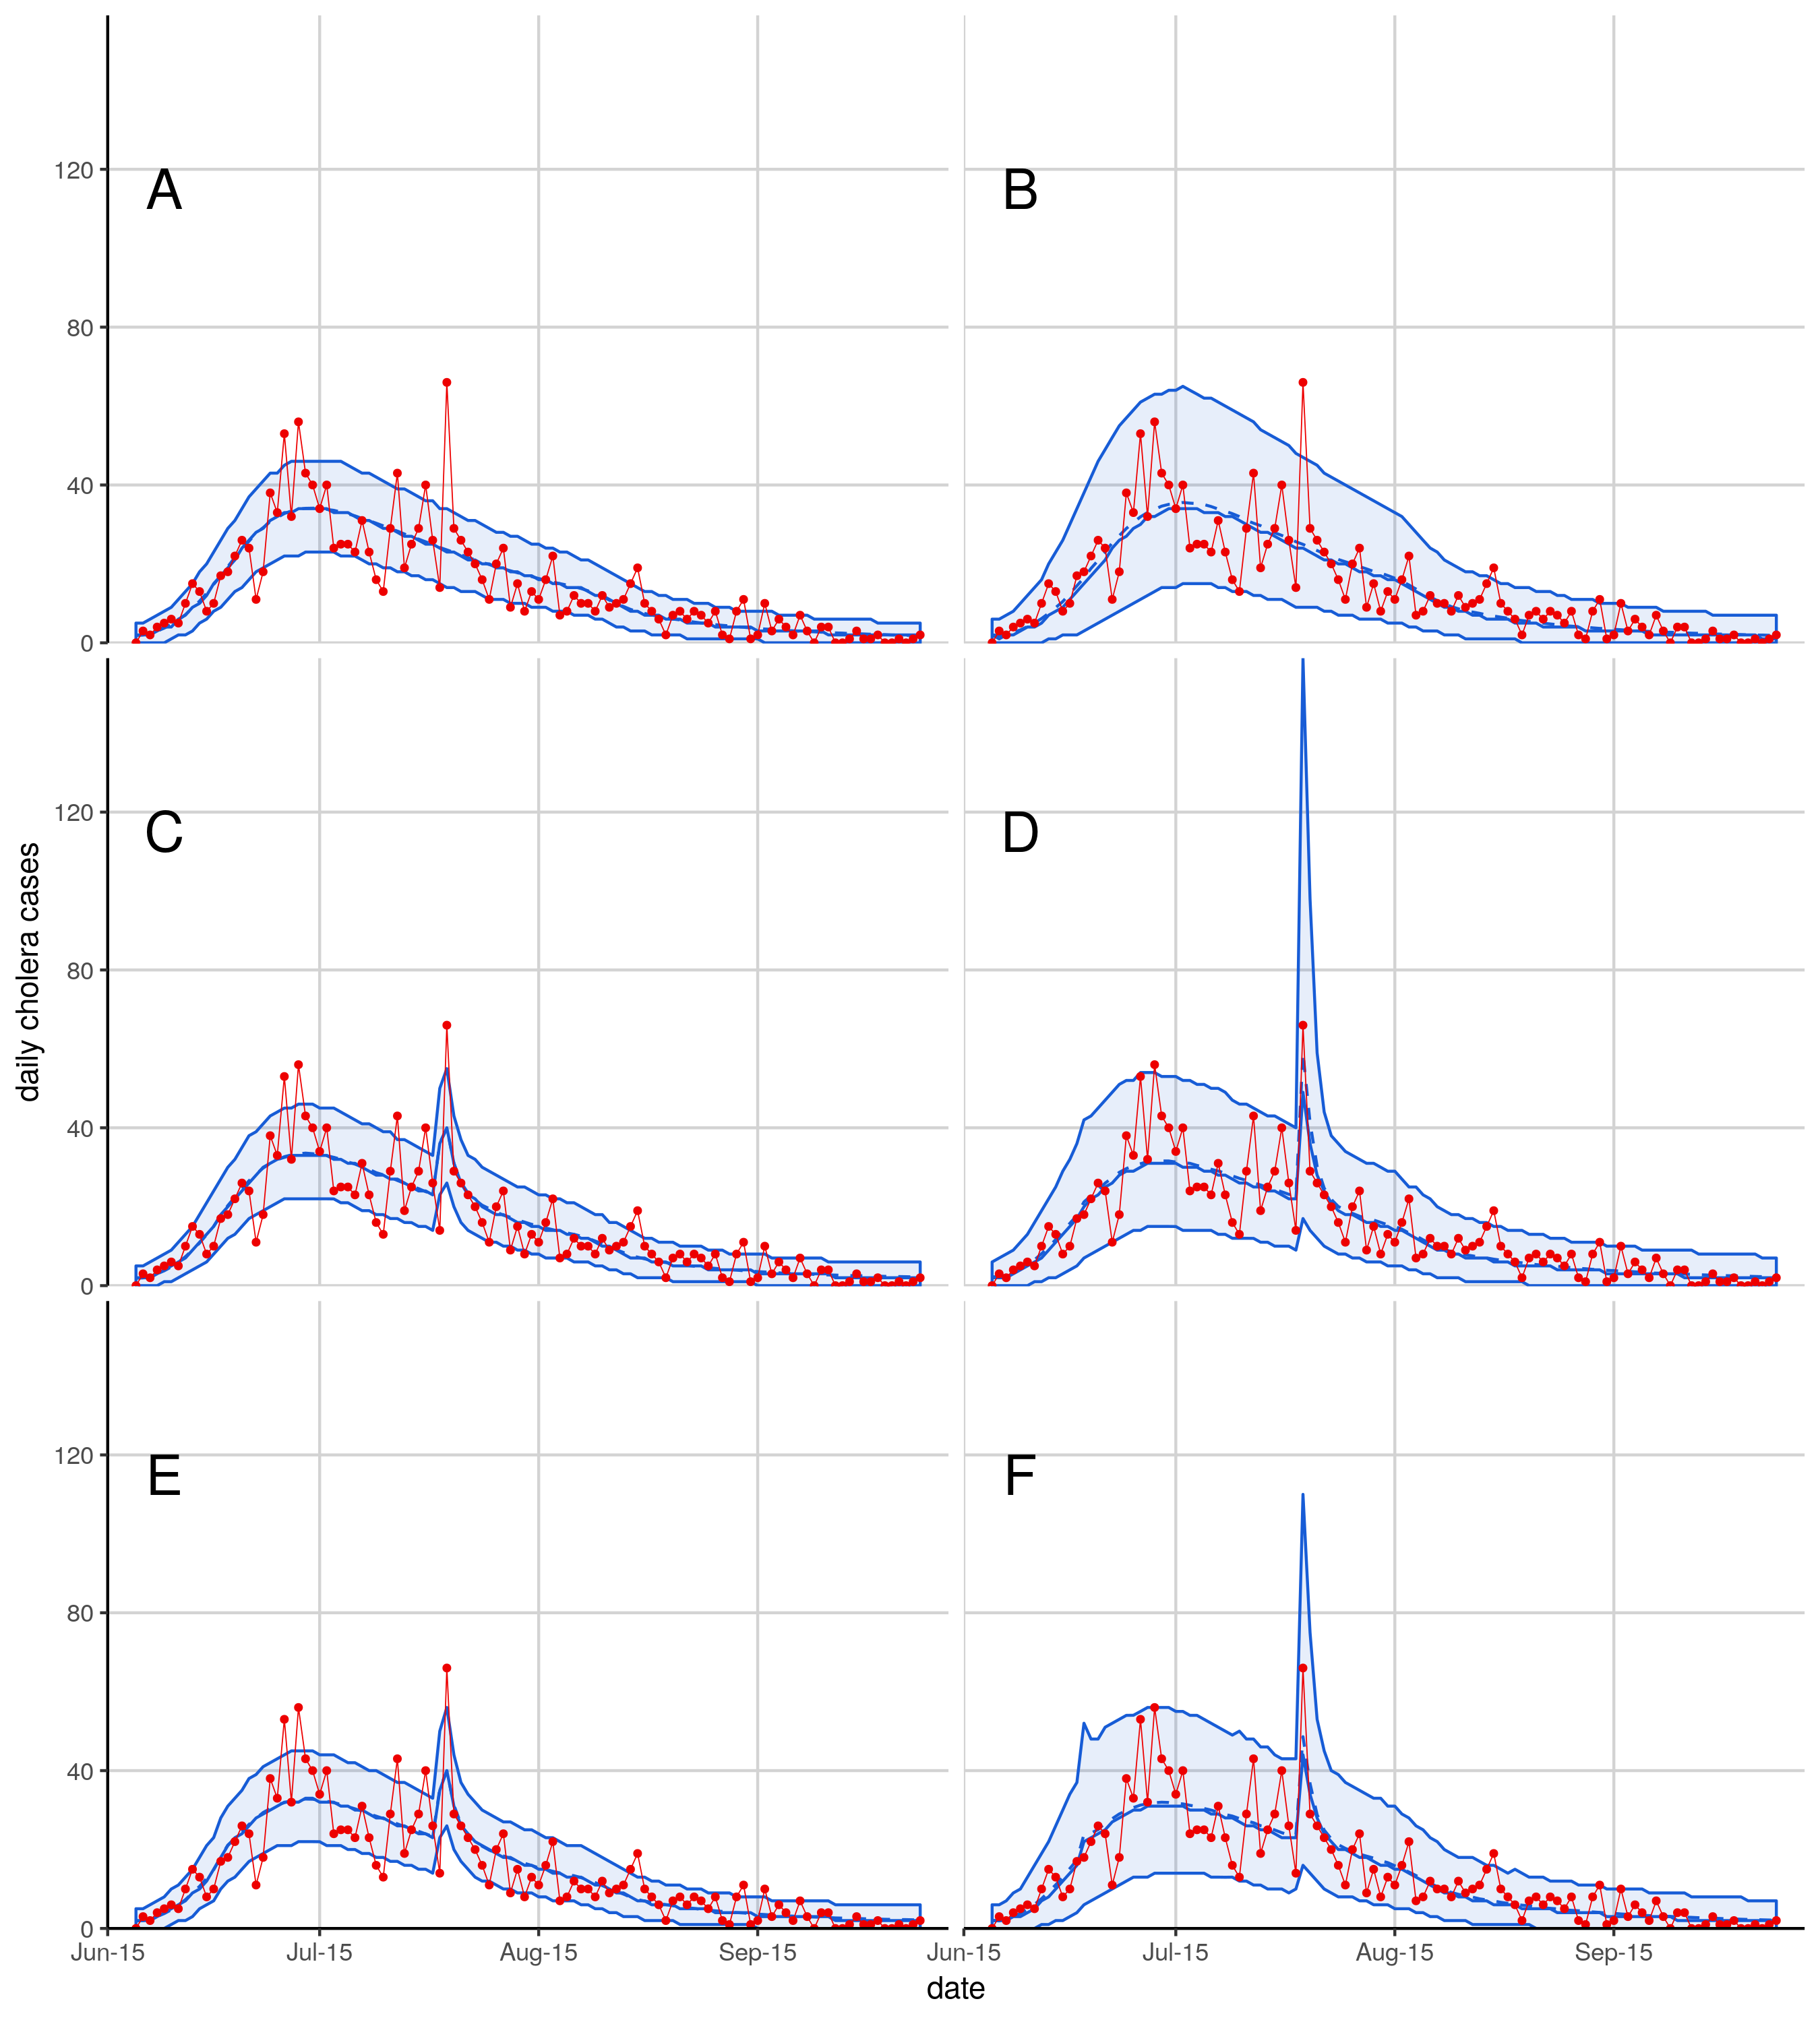
\includegraphics{fig_cholera-rainfall/Lemaitre_ACTROP_2018_42_R1_fig4.png}
    \caption[Fit of the different models]{Simulations of the \textsc{mn} (A-B), \textsc{me} (C-D) and \textsc{mec} (E-F) models. Simulations for the deterministic versions (A,C,E) are given by the mean (blue dashed line), median (blue full line) and 95\% simulation envelops (blue ribbon) of 100 simulations of the measurement model for each trajectory from 100 samples from the posteriors of model parameters against reported daily cholera cases (red line and dots). Simulations from the stochastic models (B, D, F) are given for 10'000 simulations of the stochastic process and measurement models.}
    \label{fig:sim}
\end{figure}

Comparing the two model types, stochastic results have a larger 95\% confidence interval, which better encompass most of the data. In particular, both epidemiological peaks are well captured by the stochastic models, while the deterministic results systematically underestimate them. Two factors contribute to this result: the intrinsic stochastic nature of the model, that requires the simulation of various model runs for the same set of parameters, and the noise that necessarily perturbs the force of the infection yielding an overdispersion in infections. The standard deviation of such (assumed white) noise is estimated in each stochastic model, and it is interesting to note that the MLE obtained for \textsc{ME} is slightly smaller than in \textsc{MN} (0.028 versus 0.022), highlighting again that the data are retrieved with a lower uncertainty when rainfall is included in the model. This is evident in fig.~\ref{fig:sim}, where the width of the 95\% confidence interval of models \textsc{me} and \textsc{mec} is smaller with respect to \textsc{mn}.

Finally, despite having different BFs, the deterministic models \textsc{me} and \textsc{mec} are qualitatively similar in terms of output response, indicating that the recorded changes in the log-likelihood function do not correspond to qualitative changes in the output.

\section{Discussion}
\label{sec:disc}

In this chapter, a general mechanistic SIRB-based epidemiological model is developed to evaluate the relevance of rainfall in the amplification of cholera transmission, focusing on the 2015 Juba outbreak. Two rainfall-based transmission processes were compared: the direct increase of the exposure to the contaminated water (model~\textsc{me})\cite{Eisenberg:ExaminingRainfallCholera:2013}, and the increase of water contamination by flooded open defecation sites (model~\textsc{mc})\cite{Rinaldo:Reassessment20102011:2012}. In addition, human-to-human transmission is considered (models' name with \textsc{H}).

Regarding the epidemiological model, this study introduced two innovations with respect to previous modeling attempts of cholera epidemics\cite{Bertuzzo:ProbabilityExtinctionHaiti:2016,Pasetto:RealtimeProjectionsCholera:2017}. First, the focus on daily incidence data, as opposed to weekly epidemiological reports commonly used in cholera studies, motivated the introduction of a compartment of exposed individuals, eqn.~\eqref{eq:E2j}, to account for the incubation period of the disease and, thus, the lag between the possibly rainfall-driven infection process and the manifestation of the symptoms resulting in the timeseries of daily reported cases at our disposal. %Such compartment had not been considered in previous cholera modelling works because they were most often working with weekly case reports. It was deemed necessary in this study to properly align the daily rainfall forcing with the daily reported cases.
Second, a non-linear version of rainfall driver, in the form of a power-law controlled by a single parameter, was introduced to generalize the previous linear dependence. Such formulation has the flexibility to either emphasize the impact of the largest rainfall events, or give equal weight to all non-zero rainfall intensities. %Suffice here to mention that the added parameter is properly discounted in the formal model comparison carried out here.  
%The idea is that large rainfall events may have a larger role in the deterioration of the sanitation conditions and, thus, in increasing the risk of transmission. The power low used for this goal allows, trough its parameter $\alpha$, to emphasize large precipitation events or to flatten the effect for all precipitation. 

All model assumptions were compared for both deterministic and stochastic model's types, in order to draw more general conclusions. The statistics and tests used to compare the model results  (tab.~\ref{tab:stats} and fig.~\ref{fig:lltests}) supported the significance of rainfall effects during the 2015 epidemic in Juba. In fact, results showed that for both model types there exists a significant positive effect of including rainfall drivers, in particular because standard SIRB models were not able to reproduce the second epidemiological peak of reported cases occurred in July during the recession period. All models considering rainfall, instead, showed an increase of the number of cases in correspondence of the second peak, which was due to the large rainfall rates occurred during the previous days (fig.~\ref{fig:sim}). 
This difference in the simulated responses of models considering (or not) rainfall lead to stronger support for rainfall-based models. Due to the small variations among the likelihoods of rainfall-based models, however, it is not straightforward to draw conclusions on the best way to include the rainfall effect (tab.~\ref{tab:stats}).
Models with the minimum BIC were those considering the increase in exposure (model \textsc{me}) for both the stochastic and the deterministic model types. For the deterministic models, the computation of the Bayes Factors (BFs), which should provide a direct estimation of the model probability, suggested the selection of the model combining exposure and contamination processes (model \textsc{mec}). However, this information criterion might be unstable due to numerical issues and oscillations in the \textsc{mcmc} used for calibration\cite{Raftery:EstimatingIntegratedLikelihood:2007}. By considering the fact that the models' outputs were similar for \textsc{mec} and \textsc{me} (fig. \ref{fig:sim}), it is advised to select the approach endowed with less parameters\footnote{in an attempt to maximize the model predictive accuracy we want to reduce potential overfitting.}, in this case~\textsc{me}, as indicated by the BIC. Note that the inclusion of human-to-human transmission was not statistically relevant in this modeling exercise.

\marginnote{It is also possible that the stochastic model has benefitted from improved indentifiablity. It has been shown that stochastic models can often extract more information about parameters than deterministic counterparts, see: 
\fullcite{Browning:IdentifiabilityAnalysisStochastic:2020}.}
The comparison between the likelihoods of the two models' types (deterministic and stochastic) showed that considering the stochasticity of the processes improves the model results (tab.~\ref{tab:stats}). This suggests that also deterministic models should include a stochastic term in the computation of the force of infection, eqn.~\eqref{eq:force2}, which might increase the flexibility of the outputs.

Several limitations should be considered when analyzing the present results. The calibration exercise attempted in this study considered daily rainfall and cholera reported cases, which are characterized by significant random fluctuations that might partly cloud the description of the underlying infection processes. 
Small random delays in reporting could change the infection curve and thus the effect of rainfall. This issue was partially addressed by considering the exposed compartment, eqn. \eqref{eq:E2j}, for simulation of the incubation period, and unknown reporting rate $\epsilon$ for the observed cases.

Here, it is aimed to reproduce the epidemic by modelling epidemiological transmission processes. %As usual for modelling studies, the level of description of such processes is chosen by balancing model complexity and accuracy: an increase in the number of modelled processes results in a larger number of unknown parameters, and thus a more complex calibration of the model.
While non-linear rainfall effects and possible over-reporting are taken into account, human mobility effect\cite[-4\baselineskip]{Gatto:GeneralizedReproductionNumbers:2012,Bertuzzo:SpatiallyExplicitModels:2010,Mari:PredictiveAbilityMechanistic:2015,Perez-Saez:ClimatedrivenEndemicCholera:2017} is not considered, which could help modeling the importation of infected individual.  Moreover, in this model asymptomatic infected individuals do not contribute transmission. From a modeling viewpoint, these unaccounted processes were compensated by the calibration procedure, at the loss of predictive power.

The prior bounds to be assigned to parameters are typically wide\cite{Akman:ExaminationModelsCholera:2016} because the rates governing transmission processes are highly dependent on the specific epidemiological context, so that somewhat contradictory values had been estimated in literature. These considerations, together with the intrinsic noise affecting recorded cases, underlie the possibility that some of the model parameter might be unidentifiable\cite{Eisenberg:IdentifiabilityEstimationMultiple:2013}, in the sense that different parameter combinations would yield the same model output (also called equifinality). 
The exploration of the posterior parameter distribution using an \textsc{mcmc} approach allowed us to evince the possible correlation among parameters that were well identified by the data, with the main risk of the algorithm getting trapped in a local minimum of the fitness landscape (the distribution of parameters). The posterior probability distributions of the model parameters (see the postprint supplementary information, Section S4) are associated with the model uncertainty, and were here explored by the chains of the \textsc{mcmc} calibration.

The lack of available data prevented us to include the effects of the overall efforts towards WaSH improvement in this study, but vaccination is implemented in order to eliminate one possible covariate of the rainfall effect. 
Despite these limitations, the proposed model comparison using both a deterministic and a stochastic model gave coherent results. The agreement of the two modeling types strengthened the results regarding the importance of rainfall patterns to significantly affect the development of cholera cases in time.

Overall, the findings of the study are consistent with the lessons learned in South Sudan with most of the transmission starting with the onset of the rainy season. In 2016 and 2017, cases in the dry season were observed and associated to the overexploitation of scarce water resources by nomadic herdsmen. This suggests that, as already observed, a general assessment of the relationship between precipitation and general waterborne or water-based disease infections is far from obvious and surely case-dependent. It has been argued, for example, that in the domain of water-based parasitic infections rainfall could not only boost disease transmission but also reduce it substantially\cite[-12\baselineskip]{McCreesh:ChallengesPredictingEffects:2013}, e.g. by increasing water flow (which in turn decreases habitat suitability in water). Rainfall patterns may also drastically affect human activities related to water contacts, thus potentially altering exposure and transmission risk\cite{Lai:SpatialDistributionSchistosomiasis:2015}. To that end, a hydrology-driven assessment cannot ignore certain characteristics, in particular the ephemeral or permanent nature of the waterways fostering contacts among pathogens and hosts\cite{Perez-Saez:HydrologyDensityFeedbacks:2016}. Also, temporal fluctuations of rainfall patterns may be particularly important in determining the seasonality of transmission\cite{Bertuzzo:HydroclimatologyDualpeakAnnual:2012,Bertuzzo:PredictionSpatialEvolution:2011,McCreesh:PredictingEffectsClimate:2015,Perez-Saez:HydrologyDensityFeedbacks:2016}.


%Subsuming the results obtained by this major computational exploration focused on the analysis of Juba's 2015 epidemics, it is concluded that rainfall patterns are fundamental drivers for epidemic cholera models, whether deterministic or stochastic, not only to capture seasonal trends, but also to describe short-term fluctuations in the number of reported cases. 

 % 2
%\begin{fullwidth}
\chapter[Estimating the probability of eliminating cholera from Haiti through a mass vaccination campaign]{Estimating the probability of \\ eliminating cholera from Haiti \\ through a mass vaccination campaign}%Spatial stochatic model for modeling\\cholera elimination through mass vaccination campaigns}

This chapter describes a model developed for a multi-modelling study. Four teams with existing experience in modeling cholera in Haiti were tasked to model scenarios of mass vaccination administration towards cholera immunity. The timing was meant to take advantage of the low incidence to affect the endemicity of cholera in Haiti in order to achieve elimination. The multi-model study was led by Elizabeth C. Lee and has been published as:

	\longfullcite{Lee:AchievingCoordinatedNational:2020}%\footnote{ECL, ASA, JL, and LCI conceived of the study and contributed to project administration. ECL, DLC, JCL, and LM did the primary modelling analysis, and ECL, DLC, JCL, LM, DP, JP-S, and FF wrote the model supplements. FF, RT, KV, and LCI contributed to data collection. ECL and JL wrote the first draft of the report. ECL, DLC, JCL, LM, DP, JP-S, JDS, FF, MEH, IML, ASA, JL, and LCI contributed to the study design, and all authors contributed to data interpretation and revision of the report.}. 


For this collaborative effort, a hidden Markov model of cholera transmission is developed, with specific modeling choices to account for vaccination and to gather information on elimination timing and probability.
The present chapter is adapted from Supplement 3 of the aforementioned publication, which focuses on the model designed by our team. The reader is referred to the publication by Lee et al. for the modeling exercise results and the comparison between models predictions.
\label{ch:cholera-haiti-ocv}
\end{fullwidth}


\paragraph{Cholera in Haiti} In January 2010, an earthquake hit Haiti, disrupting healthcare and water infrastructure and displacing a million persons. Ten month later, Cholera (\textit{V. Cholerae} of serogroup O1, serotype Ogawa and biotype El Tor) was introduced in Haiti by United Nation peacekeeper soldiers\cite[-3\baselineskip]{Frerichs:NepaleseOriginCholera:2012, Piarroux:UnderstandingCholeraEpidemic:2011}. 
This introduction in a naive population caused a major outbreak, totalling 820'000 reported cases and 10'000 death, most of them occurring in the first two years\cite[-1\baselineskip]{Barzilay:CholeraSurveillanceHaiti:2013}.  Since 2016, cases decreased steadily and finally the last cholera (culture) confirmed case occurred in early 2019\cite{Mitchell:PAHOWHOHaiti:2020}. Cholera exhibited a seasonal pattern with two annual peaks, and spread in every department of the country (fig. \ref{fig:data2}).
\begin{figure*}
	\centering
	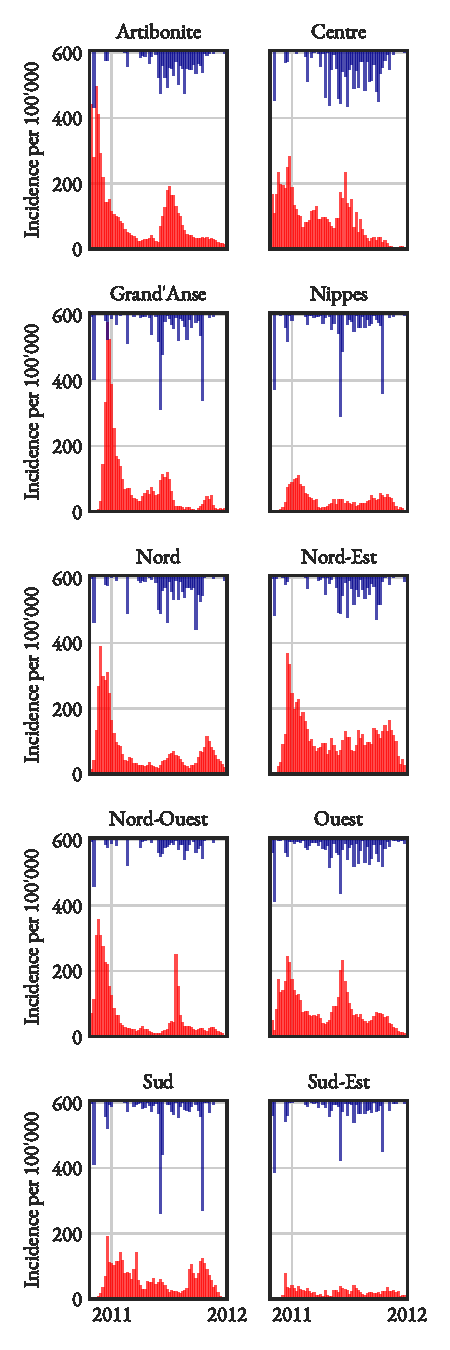
\includegraphics[height=11cm,keepaspectratio]{fig_cholera-haiti-ocv/haiti-2010.pdf}
		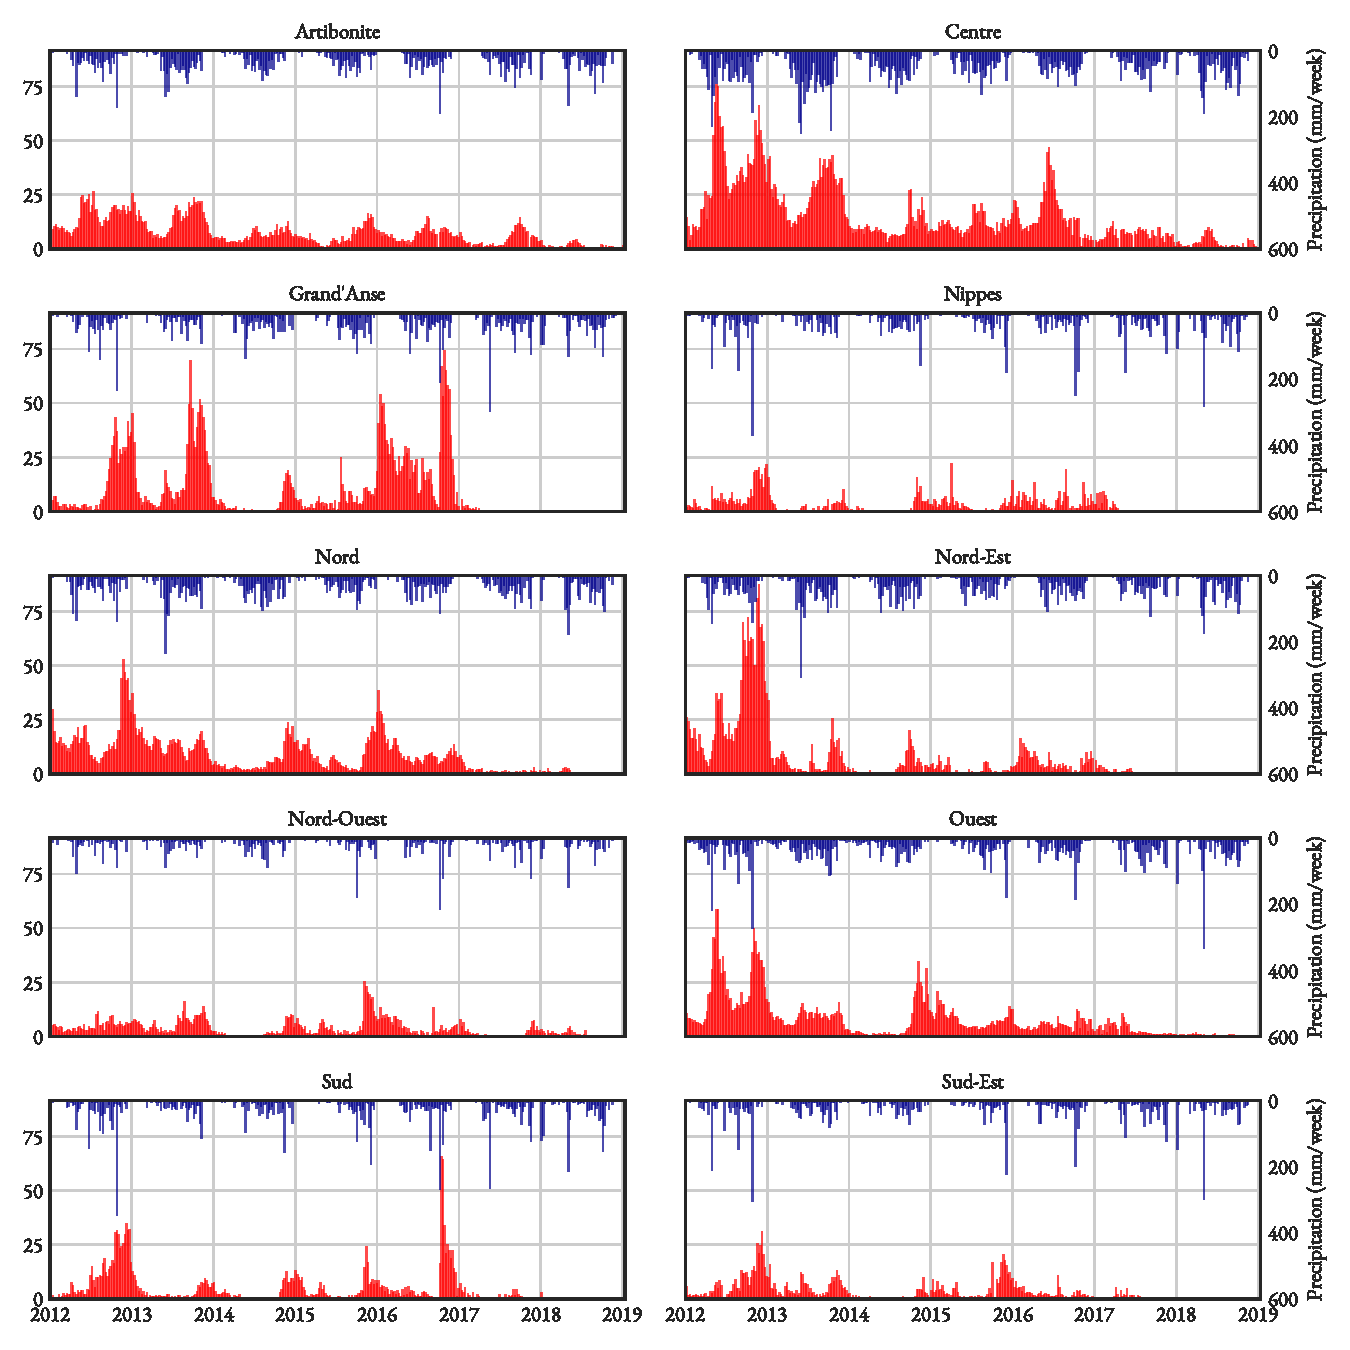
\includegraphics[height=11cm,keepaspectratio]{fig_cholera-haiti-ocv/haiti-2012.pdf}
	\caption[Incident cholera cases and rainfall in Haiti from 2010 to 2019]{Weekly incident cases and rainfall in the ten departments of Haiti from 2010 to 2019. Note that the first two years are shown with a different scale. The ressurgence in 2016 is linked to hurricane Matthew \parencites{Pasetto:RealtimeForecastingCholera:2018,Khan:AssessmentRiskCholera:2017}. The seasonality pattern is evident especially in Artibonite.}
	\label{fig:data2}
\end{figure*}


\section{Description of the model}
% Describe structure of their model and make appropriate references to their previous work. Ideally this will include at least one diagram illustrating the assumed natural history of disease and how vaccination works within the model and appropriate ODE/PDEs

\paragraph{General principles} The cholera model adopted to study the Haitian epidemic is a stochastic compartmental model applied at the level of the ten Haitian departments. 
The model is based on a Partially-Observed Markov Process (POMP), simulating the stochastic transitions between compartments as discrete events. 
It is the stochastic translation of a deterministic SIRB model based on ordinary differential equations which has been extensively used to simulate the Haitian cholera epidemic in previous studies\cite[-8\baselineskip]{Rinaldo:Reassessment20102011:2012,Bertuzzo:ProbabilityExtinctionHaiti:2016,Pasetto:RealtimeForecastingCholera:2018} and is described in \textsc{Chapter~1}. % ,Camacho:PredictionCholeraDynamics:2016
The model subdivides the population of each department\footnote[][9\baselineskip]{The case data was provided for the ten departments of Haiti, so the model spatial unit was choosen to be the department. Other teams decided either the same scale, coarser (national for Lee et al.) or finer (1km grid for Chao et al.).} into compartments counting the number of individuals at the different stages of the disease. In addition to susceptible $S$, symptomatic infected $I$ and recovered individuals $R$, a compartment for infectious asymptomatic $A$ is added for the purpose of this exercise. As in previous chapters,an environmental compartment describing the bacterial concentration $B$ in the local environment is used to estimate the force of infection. Precipitation is an important environmental driver of cholera transmission\cite{Camacho:CholeraEpidemicYemen:2018}, especially in Haiti\shortcite{Rinaldo:Reassessment20102011:2012}. As done in the contamination formulation in \textsc{Chapter~2}, rainfall increases the rate at which bacteria shed by infected individuals enter the environmental reservoir and thus increases the bacterial concentration and finally the force of infection. A diagram of the model is given in fig.~\ref{figEPFL}.
\subsection{Model dynamics} 
The following cholera dynamics are included in the model:
\begin{description}
    \item[Force of Infection and mobility] The force of infection in each department contains as additional term  the number of cholera cases in the rest of Haiti. This allows for a possible introduction of cholera due to  human mobility between departments. The force of infection in each department is composed of two parts. The first is related to the local bacterial concentration of the department. The second is related to case importation from other departments through human-to-human transmission. The corresponding equation for the $i^{th}$ department reads:
    \marginnote[-5\baselineskip]{The force of infection uses indirect (water-mediated) local transmission but direct (human-to-human) transmission for mobility exchanges. One of the reasons behind this discrepancy is technical: scalability issues linked to particle depletion hinder iterated filtering performance. Thus, it becomes very hard to calibrate a spatial model. To alleviate this issue, a custom procedure has been developed (see below) that was only tractable with simple mobility link. Instead today, the choice would be to use the improved methods that have been developed for spatial inference on pomp models \parencite{Asfaw:PartiallyObservedMarkov:2021, Park:InferenceHighdimensionalImplicit:2020}.}
    \begin{equation*}
    F^i_0(t)=\beta^i\frac{B_i(t)}{1+B_i(t)}+c^i \sum_{j\ne i} (I_j(t)+A_j(t)).
    \end{equation*}
    The first term in the sum represents local transmission governed by the department-specific exposure parameter $\beta^i$ which multiplies the logistic dose-response of the re-scaled local bacterial concentration $B = B^*/K$, where $B^*$ is the unscaled concentration of vibrios and $K$ the half-saturation constant of the logistic function $\frac{B^*_i(t)}{K+B^*_i(t)}$.
    Case importation from other departments is given by the sum of the asymptomatically and symptomatically infected in department $j$, modulated by a parameter $c^i$ which represents the intensity of case introduction from other departments in Haiti  to department $i$.
    \item[Rainfall] We account for rainfall using the contamination pathway described in the previous chapters. Rainfall increases the amount of \textit{Vibrios} per infected individual that contaminate the water reservoir. In Haiti, rainfall was empirically associated with resurgence of cholera infections in many research works\shortcite{Gaudart:SpatioTemporalDynamicsCholera:2013,Bertuzzo:ProbabilityExtinctionHaiti:2016,Adams:HaitiPreparesCholera:2012,Periago:EliminationCholeraTransmission:2012,Adams:CholeraHaitiTakes:2013,Rinaldo:Reassessment20102011:2012,Eisenberg:ExaminingRainfallCholera:2013,Kirpich:CholeraTransmissionOuest:2015}
    \item[Symptoms] A proportion $\sigma$ of infected individuals become symptomatic, and $1-\sigma$ remain (shedding, hence infectious) asymptomatic and transitions into compartment $A$ (instead of $R$ in previous chapter, because past model formulation did not account for shedding asymptomatic).
    \item[Shedding] Both symptomatic and asymptomatic infected individuals shed bacteria. The shedding rate of asymtomatics, $\theta_A$, is modeled as a fraction of the shedding rate of symptomatic individuals  $\theta_I$\cite{Kuhn:GlucoseNotRiceBased:2014}.
    \item[Recovery rate] The recovery rate is the same for both asymptomatic and symptomatic individuals ($\gamma_I=\gamma_A=0.2$ d$^{-1}$)\cite{Kaper:Cholera:1995, Codeco:EndemicEpidemicDynamics:2001}.
    \item[Acquired immunity] Individuals acquire natural immunity and remain in the recovered compartment ($R$) for a period that lasts for $1/\rho=$ 8 years on average, before reintegrating the susceptible compartment\footnote{This was surprisingly consistent across teams, with values ranging from 5 to 8 years.}.
    \item[Erlang-distributed immunity loss] To model extinction through coordinated immunity, it is needed to better approximate distribution that typically characterizes the duration of immunity\cite{King:InapparentInfectionsCholera:2008}. Instead of a exponential distribution, recovered individuals pass through a succession of three separate recovered compartments ($R_1$, $R_2$, $R_3$) characterized by the same transition rate $\rho_1=\rho_2=\rho_3=3\rho$. Hence the duration of immunity is Erlang-distributed.
    \item[Bacterial dynamics] The size of the bacterial reservoir is proportional to the population density $D_i$ of the department. This is another difference with respect to past models which used population. The goal is better capture the risk posed by cholera in slums and dense urban areas such as Port-au-Prince. Bacteria die at rate $\mu_B$ (with a mean persistence, calibrated, of less than three days). Rainfall influences the bacteria concentration by increasing the rate at which bacteria enter the environmental reservoir.
    \item[Reporting process] The reported cases are modelled by a negative-binomial distribution with dispersion parameter $p$. Over- or under-reporting is accounted for through the reporting parameter $\epsilon$.
\end{description}
    
    
\paragraph{Stochasticity} Overdispersion in the infection process is introduced by multiplying the force of infection $F_0$ by a time-continuous white noise process \(\xi(t)\) defined as the differentiation of an integrated noise process \(\xi(t) = \frac{d}{dt}\Gamma(t)\), here taken to be have a Gamma distribution with mean \(\Delta t\) and variance \(\sigma^2 \Delta t\)\cite[-3\baselineskip]{Breto:CompoundMarkovCounting:2011}:

\[
\xi(t) = \Gamma (t+\Delta t) - \Gamma (t) \sim \text{Gamma}\left( \frac{\Delta t}{\sigma^2}, \sigma^2\right).
\]

Since \(\xi(t)\) is non-negative it can serve as a multiplicative noise on
the force of infection: \[
F_i(t) = F^i_0(t) \xi(t),
\]
which yields to over-dispersion in the transitions.
%\(\Delta N_{SE}(t), \Delta N_{SR}(t), \Delta N_{V^SV^E}(t), and \Delta N_{V^SV^R}(t)\).

\begin{figure}%[htbp]
\begin{center}
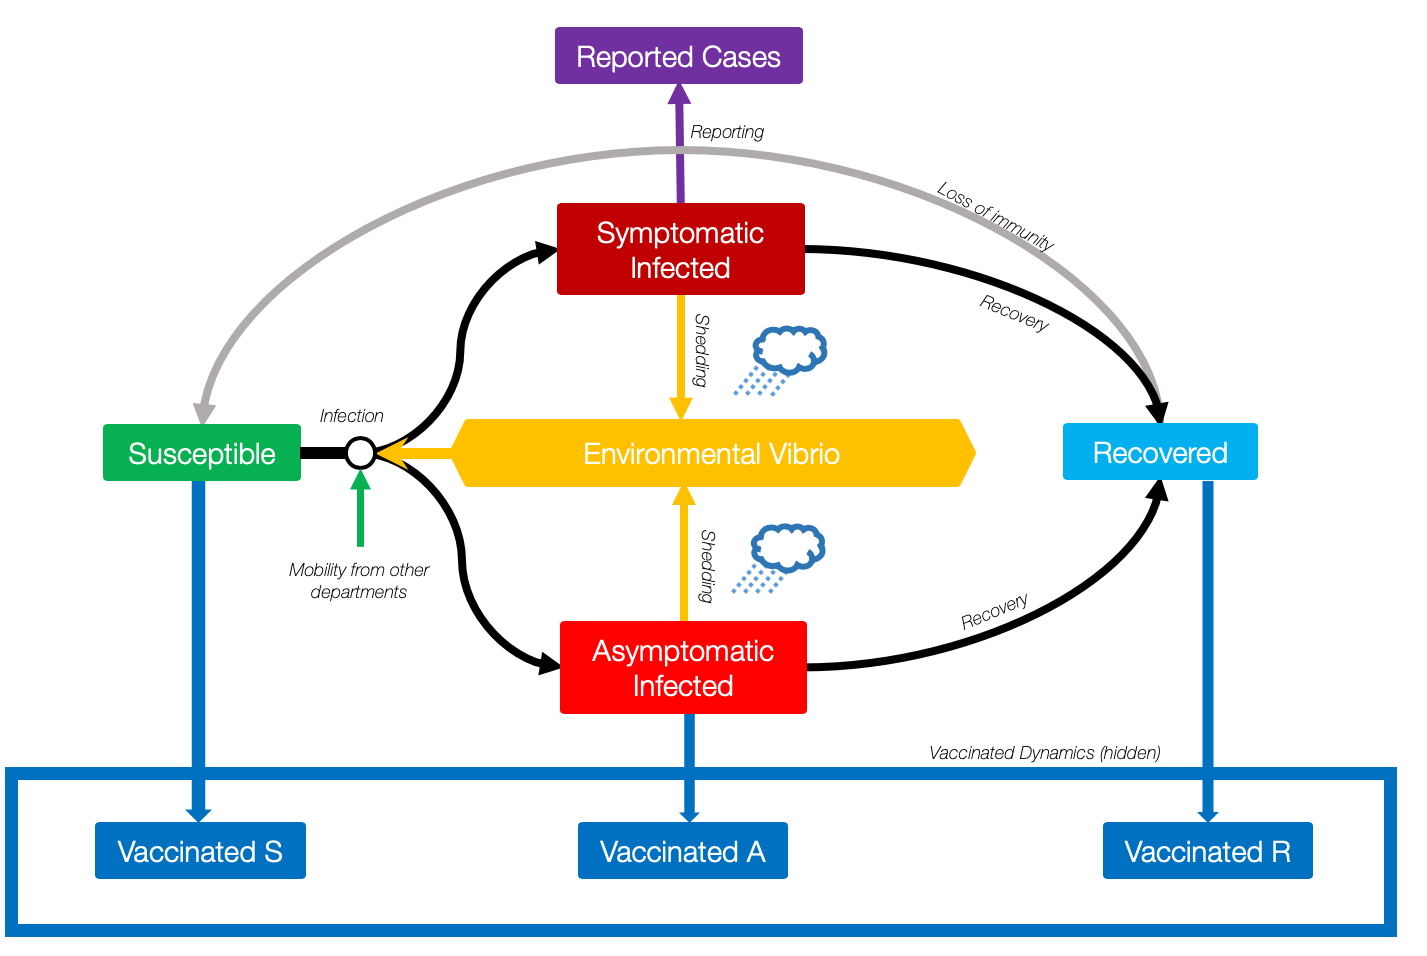
\includegraphics{fig_cholera-haiti-ocv/compartiments.png}
\caption[Schematic diagram of the cholera transmission processes in a single department]{Schematic diagram of the cholera transmission processes in a single department. Dynamics of vaccinated compartments are not shown.}
\label{figEPFL}
\end{center}
\end{figure}

\paragraph{Vaccination dynamics} The estimated vaccine efficacy was waning from 76\% over 60 month for adults, and conservatively assumed to provide no protection after 5 years. These assumptions were shared across modeling teams. 
At each vaccination campaign, the available vaccine doses are uniformly distributed among susceptible $S$, asymptomatic infected $A$ and recovered $R_{1}$, $R_2$, $R_3$ individuals. The rate of vaccination is denoted with $r_V$. Individuals can receive either one or two doses of OCV, which yield efficacies of $\eta_{1d}(t)$ and $\eta_{2d}(t)$, respectively. These parameters are common across modeling teams and the reader is reffered to the manuscript for their time-varying values. There is no age structure but the efficacy is set to be the population-weighted average of estimated efficacy for those under 5 years old and those over 5 years old.
 The model considers ten additional compartments for each vaccination campaign, in order to distinguish among individuals who received one (compartments $V^S_{1d}$, $V^A_{1d}$, $V^{R_k}_{1d}$, $k=$1, 2, 3) or two (compartments $V^S_{2d}$, $V^A_{2d}$, $V^{R_k}_{2d}$, $k=$1, 2, 3) doses of OCV. Vaccinated susceptible individuals ($V^S_{1d}$ and $V^S_{2d}$) have a lower probability to become infected (and thus entering classes $I$ or $A$) than non-vaccinated susceptibles. This is modeled through the multiplicative reduction of the force of infection by a  factor $(1-\eta_{1d}(t))$ or $(1-\eta_{2d}(t))$ respectively.
The vaccination campaign window is split equally between departments (i.e for a vaccination campaign of 5 years duration, each department will be vaccinated during a 6 month period). Vaccine efficacy starts waning after the first half of the duration of the department's vaccination campaign. For example, if for department $i$ the vaccination campaign $j$ spans from $t^{i,j}_a$ to $t^{i,j}_b$, then:
    \begin{equation}
\eta^{i,j}(t) = \left\{
    \begin{array}{ll}
        \eta_0(0) & \mbox{if t $<  t^{i,j}_a + \frac{t^{i,j}_b - t^{i,j}_a}{2}$} \\
        \eta_0(t -  (t^{i,j}_a +  \frac{t^{i,j}_b - t^{i,j}_a}{2}) ) & \mbox{if t $>  t^{i,j}_a + \frac{t^{i,j}_b - t^{i,j}_a}{2}$} \\
    \end{array}
\right.
\end{equation}
where $\eta_0(t)$ is the scenario dependant vaccine efficacy as defined in the meta-supplement.
The rates at which individuals leave compartments $V^A$ and $V^{R_k}$ ($k=$1, 2, 3) are equivalent to $A$ and $R_i$. Individuals enter the compartment $V^S$ with a vaccine efficacy reduced according to the amount of time they spent in $V^A$ and $V^{R_k}$. The actual deployment of the vaccine doses in shown in fig.~\ref{fig:deploy}.

\paragraph{Other interventions} WaSH and other intervention efforts are not explicitly considered in the model, but their impact is implicitly taken into account by calibrating the exposure rates $\beta^i$ to disease incidence that occurred while interventions were taking place. $\beta^i$ is modelled to be constant in time, meaning that changes in number or type of interventions or population behaviour over time are not taken into account. %The goal is to see if elimination is possible independently of WaSH improvement. for discussion


\subsection{Model equations}\label{sec:stoch}
The model is implemented as a stochastic counting process\cite{Breto:TimeSeriesAnalysis:2009}. Let \(N_{AB}(t)\) be the number of individuals transiting between compartments \(A,B\in \mathcal{X}\) in the time interval \([0,t)\)  where $\mathcal{X}$ is the state vector,
$$\mathcal{X} = \{S, I, A, R_k, V^S_{j,1d},V^A_{j,1d}, V^{R_k}_{j,1d}, V^S_{j,2d},V^A_{j,2d}, V^{R_k}_{j,2d}\} 
\text{ for } j = 1, ..., J, \text{ and } k = 1, 2, 3,
$$
%\marginnote{The model formalism is similar to the one used for the stochastic model in \textsc{Chapter~2} and detailled in the \textsc{Appendix}, eqn. \eqref{eq:stochsys}.}
and $J$ is the number of vaccination campaigns in the department.
The number of transitions during a time-step $\Delta t$ is
\(\Delta N_{AB}(t) = N_{AB}(t+\Delta t) - N_{AB}(t)\). Given the state of the system at time \(t\), \(\mathcal{X}_t\), and a force of infection $F_j(t)$ the transition rates read (transitions are written only for one dose of OCV and one vaccination campaign to shorten the equations):
\begin{fullwidth}
\begingroup
\allowdisplaybreaks
\label{eq:stochsys}
\begin{align}
    \mathbb{P}\left[ \Delta N_{SI}(t) = 1 \mid\mathcal{X}_t\right] &= \sigma F_j(t) S(t) \Delta t + o(\Delta t)\\ \label{eq:stochstart}
    \mathbb{P}\left[ \Delta N_{SA}(t) = 1 \mid\mathcal{X}_t\right] &= (1-\sigma) F_j(t) S(t) \Delta t + o(\Delta t)\\
    \mathbb{P}\left[ \Delta N_{SV_{1d}^S}(t) = 1 \mid\mathcal{X}_t\right] &= r_{V_{1d}}(t) S(t) \Delta t + o(\Delta t)\\
    \mathbb{P}\left[ \Delta N_{S\bullet}(t) = 1 \mid\mathcal{X}_t\right] &= \mu  S(t) \Delta t + o(\Delta t)\\
    \mathbb{P}\left[ \Delta N_{IR_1}(t) = 1 \mid\mathcal{X}_t\right] &= \gamma I(t) \Delta t + o(\Delta t)\\
    \mathbb{P}\left[ \Delta N_{I\bullet}(t) = 1 \mid\mathcal{X}_t\right] &= (\mu+\alpha)I(t) \Delta t + o(\Delta t)\\
    \mathbb{P}\left[ \Delta N_{AR_1}(t) = 1 \mid\mathcal{X}_t\right] &= \gamma A(t) \Delta t + o(\Delta t)\\
      \mathbb{P}\left[ \Delta N_{AV_{1d}^A}(t) = 1 \mid\mathcal{X}_t\right] &= r_{V_{1d}}(t) A(t) \Delta t + o(\Delta t)\\
      \mathbb{P}\left[ \Delta N_{A\bullet}(t) = 1 \mid\mathcal{X}_t\right] &= \mu  A(t) \Delta t + o(\Delta t)\\
    \mathbb{P}\left[ \Delta N_{R_kR_{k+1}}(t) = 1 \mid\mathcal{X}_t\right] &= 3\rho R_k(t) \Delta t + o(\Delta t),\quad k=1,2\\
    \mathbb{P}\left[ \Delta N_{R_3S}(t) = 1 \mid\mathcal{X}_t\right] &= 3\rho R_3(t) \Delta t + o(\Delta t)\\
    \mathbb{P}\left[ \Delta N_{R_kV_{1d}^{R_k}}(t) = 1 \mid\mathcal{X}_t\right] &= r_{V_{1d}}(t) R_k(t) \Delta t + o(\Delta t)\quad k=1,2,3\\
    \mathbb{P}\left[ \Delta N_{R_k\bullet}(t) = 1 \mid\mathcal{X}_t\right] &= \mu  R_k(t) \Delta t + o(\Delta t)\quad k=1,2,3\\
    \mathbb{P}\left[ \Delta N_{V_{1d}^SI}(t) = 1 \mid\mathcal{X}_t\right] &=  \sigma (1-\eta_{1d}^{i,j}(t)) F_j(t) V_{1d}^S(t) \Delta t + o(\Delta t)\\
    \mathbb{P}\left[ \Delta N_{V_{1d}^SA}(t) = 1 \mid\mathcal{X}_t\right] &=  (1-\sigma) (1-\eta_{1d}^{i,j}(t)) F_j(t) V_{1d}^S(t) \Delta t + o(\Delta t)\\
    \mathbb{P}\left[ \Delta N_{V_{1d}^S\bullet}(t) = 1 \mid\mathcal{X}_t\right] &= \mu  V_{1d}^S(t) \Delta t + o(\Delta t)\\
    \mathbb{P}\left[ \Delta N_{V_{1d}^AV_{1d}^{R_1}}(t) = 1 \mid\mathcal{X}_t\right] &= \gamma V_{1d}^A(t) \Delta t + o(\Delta t)\\
    \mathbb{P}\left[ \Delta N_{V_{1d}^A\bullet}(t) = 1 \mid\mathcal{X}_t\right] &= \mu  V_{1d}^A(t) \Delta t + o(\Delta t)\\
    \mathbb{P}\left[ \Delta N_{V^{R_k}V^{R_{k+1}}}(t) = 1 \mid\mathcal{X}_t\right] &= 3\rho V^{R_k}(t) \Delta t + o(\Delta t),\quad k=1,2\\
    \mathbb{P}\left[ \Delta N_{V_{1d}^{R_3}V_{1d}^S}(t) = 1 \mid\mathcal{X}_t\right] &= 3\rho V_{1d}^{R_3}(t) \Delta t + o(\Delta t)\\
    \mathbb{P}\left[ \Delta N_{V^{R_k}\bullet}(t) = 1 \mid\mathcal{X}_t\right] &= \mu  V^{R_k}(t) \Delta t + o(\Delta t)\quad k=1,2,3 \label{eq:stochend}
\end{align}
\endgroup
\end{fullwidth}
assuming that \(\mathbb{P}[\Delta N_{XY} > 1\mid\mathcal{X}_t] = o(\Delta t) \; \forall X,Y \in \mathcal{X}\) and \(\mathbb{P}[\Delta N_{X\bullet} > 1\mid\mathcal{X}_t] = o(\Delta t) \; \forall X \in \mathcal{X}\). Note that \(\mathbb{P}\left[ \Delta N_{X\bullet}(t) = 1 \mid\mathcal{X}_t\right]\) denotes probability that individuals die and it is governed by the same parameter $\mu$ for all compartments except $I$. 

The ensuing stochastic variations of the state variables are:
\begin{fullwidth}
\begingroup
\allowdisplaybreaks
\label{eq:stochstates}
\begin{align}
    \Delta I(t) &= \Delta N_{SI}(t) -  \Delta N_{IR_1}(t) -  \Delta N_{I\bullet}(t)\\
    \Delta A(t) &= \Delta N_{SA}(t) -  \Delta N_{AR_1}(t) -  \Delta N_{AV^A}(t) - \Delta N_{A\bullet}(t)\\
    \Delta R_1(t) &= \Delta N_{IR_1}(t) + \Delta N_{AR_1}(t) -  \Delta N_{R_1 R_2}(t) -  \Delta N_{R_1V^{R_1}}(t) -  \Delta N_{R_1\bullet}(t)\\
    \Delta R_2(t) &= \Delta N_{R_1R_2}(t) - \Delta N_{R_2 R_3}(t) -  \Delta N_{R_2V^{R_2}}(t) -  \Delta N_{R_2\bullet}(t)\\
    \Delta R_3(t) &= \Delta N_{R_2R_3}(t) - \Delta N_{R_3 S}(t) -  \Delta N_{R_3V^{R_3}}(t) -  \Delta N_{R_3\bullet}(t)\\
    \Delta V^S(t) &= \Delta N_{SV^S}(t) -  \Delta N_{V^S I}(t)-  \Delta N_{V^S A}(t) - \Delta N_{V^S\bullet}(t)\\
    \Delta V^A(t) &= \Delta N_{AV^A}(t) -  \Delta N_{V^AV^{R_1}}(t) - \Delta N_{V^A\bullet}(t)\\
    \Delta V^{R_1}(t) &= \Delta N_{R_1V^{R_1}}(t) +  \Delta N_{V^AV^{R_1}}(t) - \Delta N_{V^{R_1}V^{R_2}}(t) - \Delta N_{V^{R_1}\bullet}(t)\\
    \Delta V^{R_2}(t) &=\Delta N_{R_2V^{R_2}}(t)+\Delta N_{V^{R_1} V^{R_2}}(t) -  \Delta N_{V^{R_2}V^{R_3}}(t) -  \Delta N_{R_2\bullet}(t)\\
    \Delta V^{R_3}(t) &= \Delta N_{R_3V^{R_3}}(t)+\Delta N_{V^{R_2}V^{R_3}}(t) - \Delta N_{V^{R_3}V^ S}(t) - \Delta N_{V^{R_3}\bullet}(t)\\
    S(t) &= H_i - \sum_{X \in \mathcal{X} \backslash \{S\}} X(t),
\end{align}
\endgroup
\end{fullwidth}
where the equation for $S(t)$ enforces a constant total population. 
The rescaled bacterial concentration $B$ is necessary to estimate the force of infection and is computed using the following ODE:
\begin{equation}
\frac{dB}{dt} = - \mu_B B +  \left(1 + \lambda\left( J(t)\right)^{r} \right)  D_i \left[\theta_I I + \theta_A A\right] 
\end{equation}
where $J(t)$ is the precipitation over time and $D_i$ is the average population density of the department\footnote{total department population over department area. It is assumed that density is more important than population size, a change from the historical model described in \textsc{Chapter~1}}.  Parameter $\mu_B$ expresses the mortality rate of the bacteria in the environment, $\theta_I$ and $\theta_A$ are the shedding rates of symptomatic and asymptomatic infected individuals, and $\lambda$ and $r$ are the parameters of the power-law that controls the non-linear impact of precipitation, as in \textsc{Chapter~2}. The model was simulated with a constant time-step of $4.8$h, and the ODE for the bacterial concentration was integrated using a Runge-Kutta 4 scheme.



Let \(C(t_j)\) denote the number of people that develop symptoms and seek healthcare during the
observation interval \([t_j, t_{j+1})\) (i.e. the true incidence). Thus:

\begin{equation}
    C(t_j) = [N_{SI}(t_{j+1}) - N_{SI}(t_j)] + [N_{V^SI}(t_{j+1}) - N_{V^SI}(t_j)].
\end{equation}

Our Markov process formulation requires a measurement model linking the time series of the reported incidence to \(C(t_j)\) as the observed variable to the process model in eqn. \eqref{eq:stochsys} . A negative-binomial measurement model accounting for over- or under-reporting of cholera incidence os choosen, i.e.
\[
	\text{cases}(t_j) \sim \text{NB}(\epsilon(t) C(t_j), p).
\]
where \(\epsilon(t) > 0\) represents the proportion of cases reported. To account for the change of the case definition that occurred on January 1, 2018, the reporting rate changes over time:
\begin{equation}
\epsilon(t) = \left\{
    \begin{array}{ll}
        \epsilon_1 & \mbox{if t $<$ Jan 1st, 2018} \\
        \epsilon_2 & \mbox{otherwise}
    \end{array}
\right.
\end{equation}

The parameters of the model are shown in tab.~\ref{paramEPFL}.



% Table with all model parameters indicating whether each is fit or assumed (with some description of assumptions) and appropriate references to primary literature (please don't cite previous parameters used in modeling studies).

\begin{table*}
\caption{Model parameters%References:%\fullciteshortb{Levine:DurationInfectionDerivedImmunity:1981, Koelle:DisentanglingExtrinsicIntrinsic:2004, Bertuzzo:SpacetimeEvolutionCholera:2008, Kaper:Cholera:1995}
}
\begin{tabular}{lcccl}
\toprule
Parameter & Calibration & Value or bound & Unit & description \\
\midrule
$\beta^i$ ($\times 10$ dept.) & yes & $[0,\infty]$ & -- & Exposure  \\
$c^i$ ($\times 10$ dept.) & yes & $[0,\infty]$& -- & Force of infection in dept. $i$ from cases in other depts. \\
$\epsilon_1$& yes & $[0,2]$ & --& reporting fraction before January 1, 2018\\
$\epsilon_2$& yes & $[0,2]$ & --& reporting fraction after January 1, 2018\\
$\sigma_w$ & yes& $[0,0.1]$ & --&  std-dev of the perturbation of $F(t)$\\
$p$& yes &$[0,\infty]$ & --&  dispersion parameter of reporting\\
$\theta_I$  & yes &   $[0,\infty]$ & --& Shedding sympt.  \\
$\theta_A$  & yes &  $[0,\theta_I]$ &  --& Shedding asympt. \\ 
$\mu_B$   & yes & $[0,\infty]$ &d$^{-1}$ & Bacterial mortality in environment \\ 
$r$       & yes &  $[0,\infty]$ & --& Exponent rainfall \\ 
$\lambda$  & yes &   $[0,\infty]$ & --& Coef. rainfall \\ 
$\rho$  & no & $1/(8\cdot365)$ &d$^{-1}$ & Loss of immunity (Levine et al.,1981 and Koelle et al, 2004)\\ 
$\sigma$  & no & $0.25$ & -- & Symptomatic/exposed \\  
$\alpha$  & no &  $0.004$ & d$^{-1}$& Mortality due to cholera (Bertuzzo et al., 2008)\\ %estimated based on data in Enrico's paper
$\gamma$  & no & $1/5$& d$^{-1}$ & Recovery rate  sympt. (Kaper, 1995)\\  
$k$    & no  & $3$ & --& number of recovered compartments \\
$\mu$  & no &  $1/(63.6\cdot365)$ &d$^{-1}$ & mortality rate from life expectancy (World bank, 2017)\\  
$\eta_{1d}(t), \eta_{2d}(t)$ & no  & as in spec. & --& Vaccine efficacy for 1 and 2 doses \\
\bottomrule
\end{tabular}
\label{paramEPFL}
\end{table*}

\section{Calibration of the model}
% Description of additional data
\paragraph{Data} Remote-sensed precipitation estimates from NASA's TRMM and GPM missions are used\footnote{TRMM 3B42 RT Derived Daily Product \parencite{Huffman:TRMMMultisatellitePrecipitation:2007} is used from October 2010 to March 2015,  and GPM from from April 2015 to December 2019.}. Rainfall measurements are provided on a regular grid. To get a value for each department, the measurements are averaged over the extent of the department. The time series of future rainfall up to the year 2030 is constructed by sampling from the past 20 years of data  with replacement blocks of 15 days. To keep the correct seasonality the day of the year of each block is preserved.

\paragraph{Fitting procedure} The model is calibrated separately for each department on the weekly reported cases from March 1, 2014 to January 1st 2019. The calibration procedure is based on a frequentist multiple iterated filtering algorithm (MIF2)\cite{Ionides:InferenceDynamicLatent:2015}. The initial conditions on March 1, 2014 are derived by enforcing the model dynamics on the reported cases from the start of the epidemic in 2010. The MIF2 algorithm performance deteriorates quickly with the spatial dimension of the model as the number of particles needed for calibration increase exponentially\cite{Park:GuidedIntermediateResampling:2017}\footnote{As mentionned, new methods have addressed these limitations\parencite{Asfaw:PartiallyObservedMarkov:2021, Park:InferenceHighdimensionalImplicit:2020}}. To address this problem each department is first calibrated independently. In a second step, using the departmental calibration as a starting point, the entire spatial model is calibrated.
The department-specific calibration procedure is as follow:

\begin{enumerate}
    \item All unknown parameters are calibrated on the reported cases of Artibonite, where the epidemic had a clear seasonal dynamic from 2014 to 2018 with a sufficiently large number of cases, thus providing a good signal for the model.  This allows to calibrate the unknown epidemiological and rainfall-related parameters on the most informative time series available.
    \item For the other nine departments, the most sensitive parameters are calibrated: the exposure $\beta^i$ and the mobility parameter $c^i$ only, while fixing the remaining parameters to their best fit found for Artibonite.
    \item The large, rainfall unrelated cholera outbreak in the Ouest department in 2015--2016 (mainly Port-au-Prince)\footnote{unpublished field investigations speak of the notable contribution of the vandalism of main water pipes by gangs \parencite{Rebaudet:NationalAlertresponseStrategy:2018}.} is excluded from the calibration since it is not part of the endemic dynamics that are the focus of  this study.
\end{enumerate}

During this phase, the mobility coefficients $c_i$ are calibrated using the reported cholera cases (data) from the other departments (appropriately scaled with the reporting rate and symptomatic fraction).
\begin{figure*}[htbp]
\begin{center}
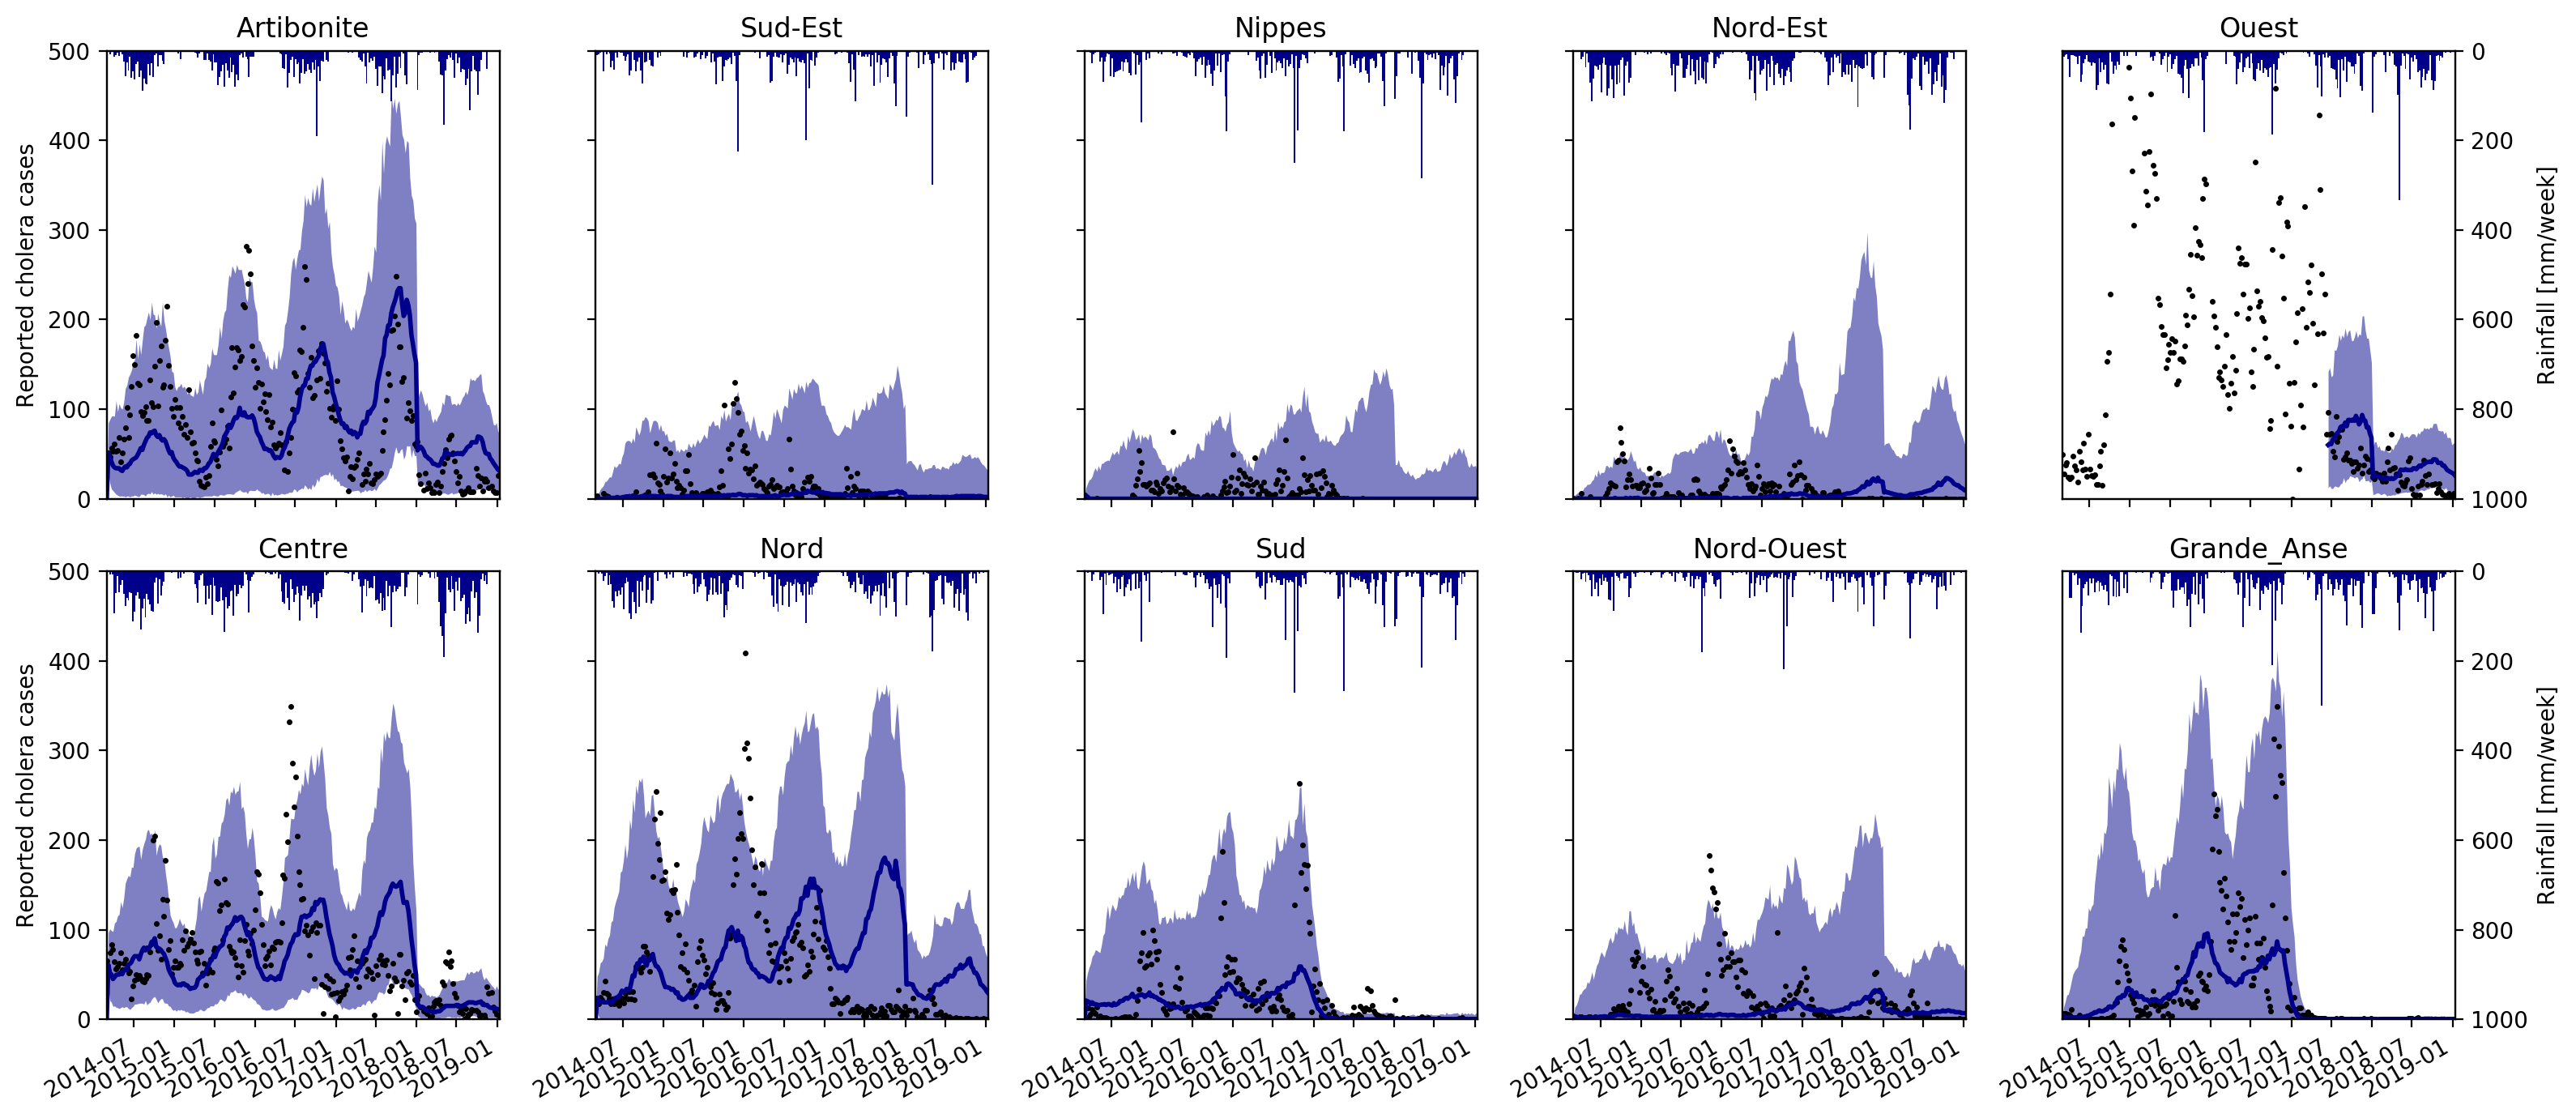
\includegraphics[width=1.0\textwidth]{fig_cholera-haiti-ocv/fit.png}
\caption[Visual assessement of model fit for the selected parameters set]{Visual assessement of model fit for the selected parameters set. The median (blue line) and the q025 and q975 quantiles (shaded area) over 1000 realization of the stochastic model are shown. Weekly reported cholera cases are shown as black dots.}
\label{fitEPFL}
\end{center}
\end{figure*}
After visual convergence is reached in each departements, the departmental best fits is taken as starting points for a country-wide calibration. This mainly affects the mobility parameter $c_i$, which governs the departmental interdependence, as it now calibrated on the actual simulated incidence from other departments. The resulting model fit is shown in fig.~\ref{fitEPFL}. 

\section{Results and discussion}
The common outputs for the exercise are the distribution of time to elimination and probability of elimination in different scenarios. The results are presented below for the six following scenarios, common across modeling teams:
\begin{itemize}
	\item \textsc{No vaccination} status quo.
	\item \textsc{National over 2 years} a nation-wide OCV campaign to reach a coverage 70\% double dose coverage, 10\% single dose and 20\% without any vaccine after 2 years.
	\item 	 \textsc{National over 5 years} a nation-wide OCV campaign with the same coverage, but with a slower deployement over 5 years.
	\item \textsc{2 Departments over 2 years} Campaign focusing only on Centre and Artibonite, the two departments with the highest recent incidence of cholera. Vaccines are deployed to reach the same coverage over 2 years.
	\item \textsc{3 Departments over 2 years} Same as above, but with the addition of Ouest department.
	\item \textsc{National over 2 years, high coverage} same as the National over 2 years, but with a much higher coverage of 95\% two doses, 1.67\% one doses and 3.33\% no vaccination.
\end{itemize}
These scenarios are summarized in in fig.~\ref{fig:deploy} in terms of cumulative number of doses deployed.

\begin{figure}
\begin{center}
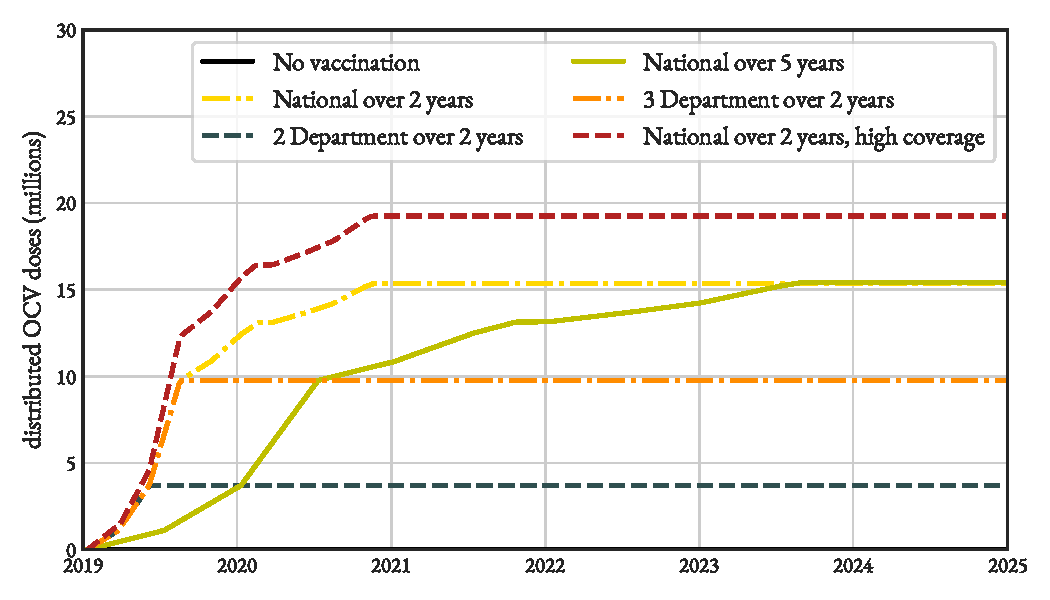
\includegraphics{fig_cholera-haiti-ocv/haiti-deploy.pdf}
\caption[Rate of vaccine doses deployment in each considered scenarios][5\baselineskip]{Rate of vaccine doses deployment in each considered scenarios.}\label{fig:deploy}
\end{center}
\end{figure}

The results in terms of probability of elimination and incidence are shown in fig.~\ref{fig:OCVresults}\marginnote{Only results from our model are presented here. Due to the difficulty of the exercise, the results across teams were quite different, and the reader is referred to \textcite{Lee:AchievingCoordinatedNational:2020} and its supplement to compare the results with the other modeling teams.}. Only a limited long-term impact of the \textsc{2 departments} scenarios is projected. However, all \textsc{national} scenarios considered were projected to lead to elimination, despite the limited vaccine efficacy and coverage. The \textsc{2 departments} and \textsc{3 departments} scenarios exhibit a probability of elimination of about 9.6\% and 48\% respectively (compared to 4.1\% in the status quo scenario). The important impact of adding Ouest to the campaign is due to the department's population, around 4\textsc{m}, which represents about 40\% of the Haitian population. While a slower timing decreases slightly the probability of elimination, it is noted that coverage is far more important than speed for these vaccination campaigns.

\begin{figure*}[h!]%[htbp]
\begin{center}
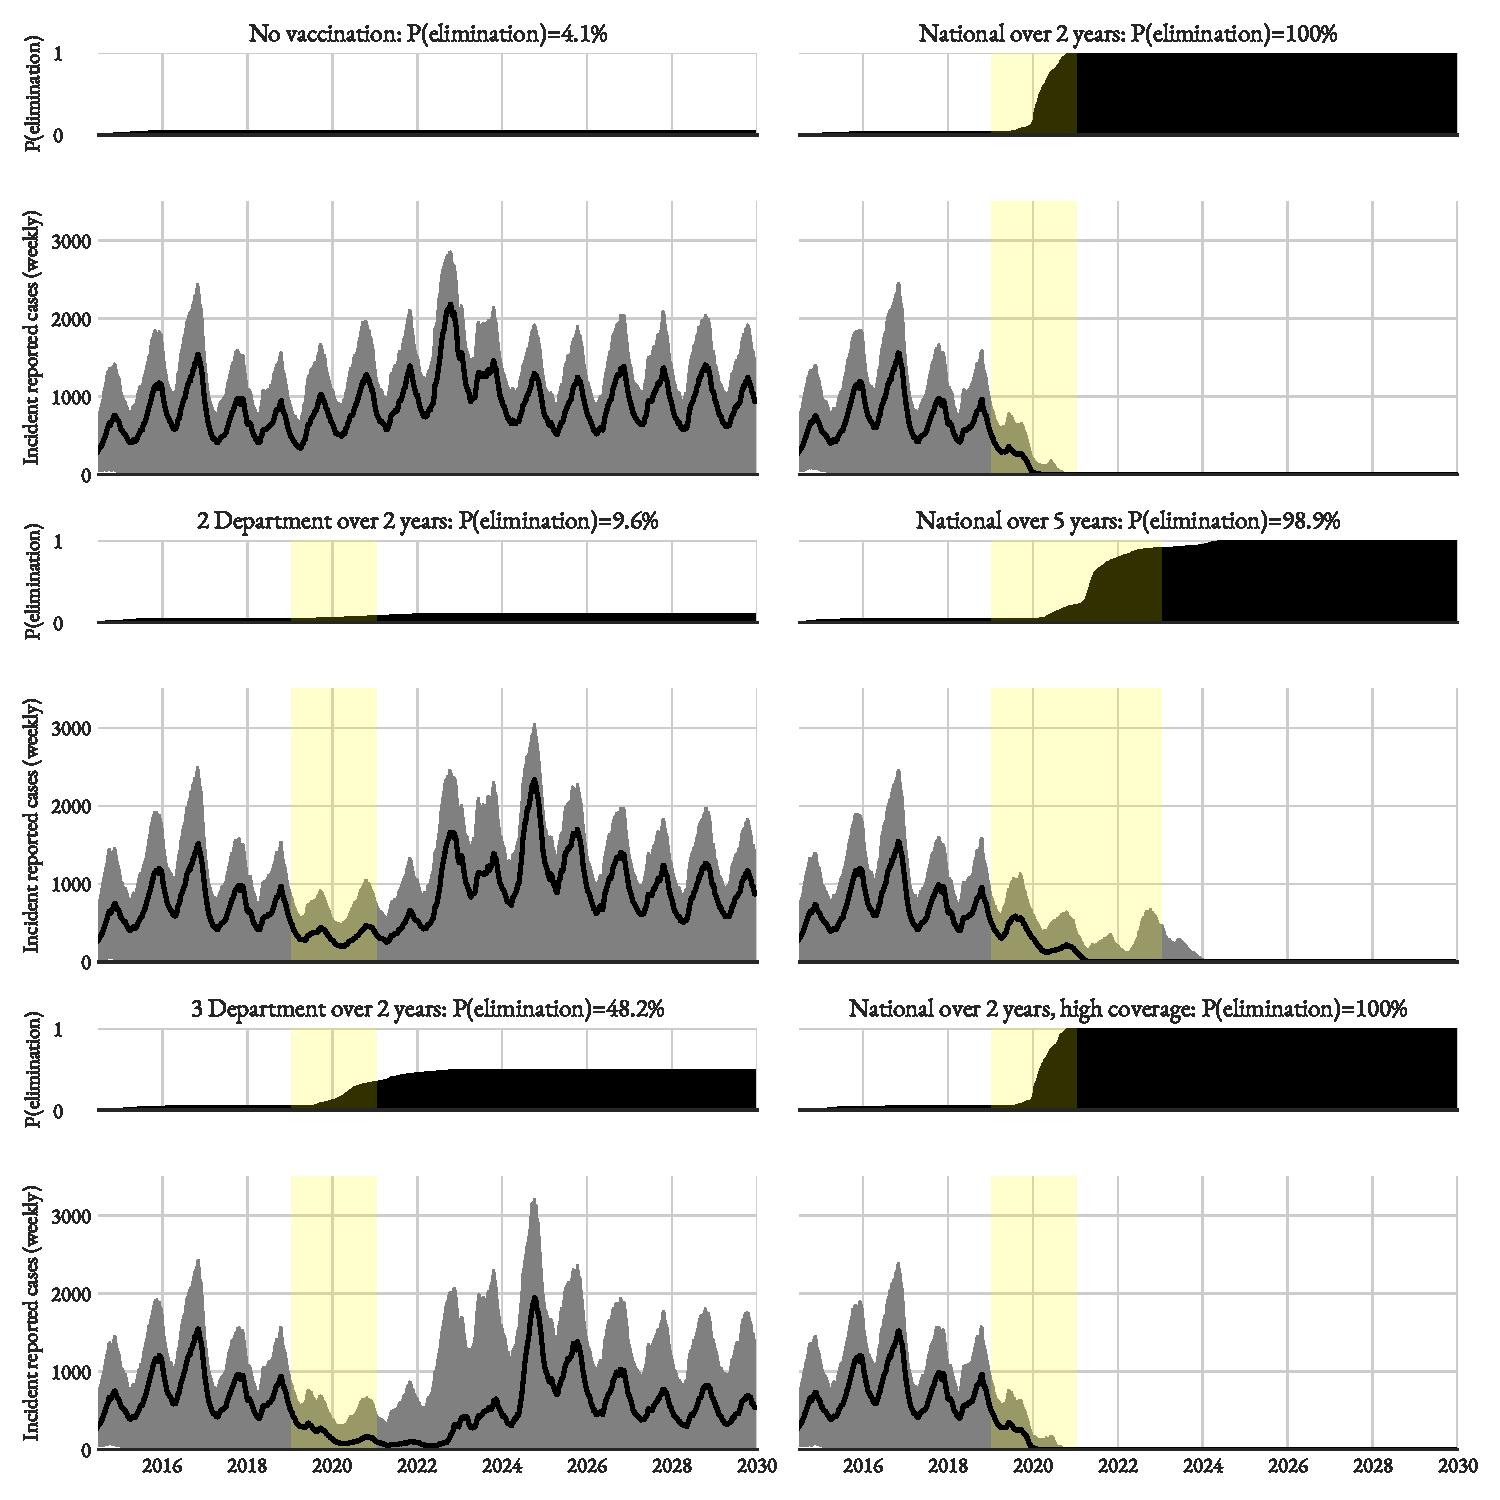
\includegraphics{fig_cholera-haiti-ocv/haiti-scn.pdf}
\caption[Model results: probability of cholera elimination after mass vaccination campaigns]{Modeling results for the considered mass vaccination campaign scenarios, with the weekly reported cases (median and 95\% confidence interval), and cumulative probability of elimination over time. The timing of the vaccine distribution in each scenario is highlighted in yellow.}
\label{fig:OCVresults}
\end{center}
\end{figure*}
 
Haiti has seen no laboratory-confirmed cases of cholera from February 2019. This has sparked claims of cholera elimination, which would mean that the Americas would be free from Cholera. However in the model results, the probability of elimination in the no vaccination scenario is very low (4.1\%). It is always very difficult to predict or explain disease transmissions, and it is even harder for elimination. Possible explanations for the discrepancy observed between what is projected by the model and what happened are (i) issues in the model design, especially concerning the mobility acting as a constant additive pressure for the introduction of cholera cases, hence lowering the probability of extinction; this was done purposefully to sustain transmission as it improved model fit and it was not believed Haiti to be close to elimination at that time, (ii) transmission parameters values error might have biased the estimate of the susceptible population on March 1, 2014, as the absence of serosurvey makes the correct estimation of this quantity critical, (iii) not giving enough weight to the decrease in reported cases from 2017\footnote[][-1.5\baselineskip]{a 90\% decrease of reporting is necessary for the model to replicate the decline in cases. However, it is highly unlikely that the observed decrease in cases is solely due to changes in the reporting process.}, (iv) WaSH interventions and rapid response teams that have been put in place in Haiti and of which have intensified in the last few years\cite{Rebaudet:CaseareaTargetedRapid:2019} might have played a role in disease elimination.
  
 Further work must be performed to study the reasons behind the surprising (to us and other modeling groups, one year before) elimination of cholera from Haiti, and to assess all factors, including WaSH interventions, environmental drivers and socio-economic changes in an unified modeling framework. Effort to investigate this (using the same methods presented for \textsc{covid}-19 in \textsc{Chapter~5}) have been started, but the project has been disrupted owing to \textsc{covid}-19 pandemic, which is the focus of the three remaining chapters.
  % 3
%\begin{fullwidth}
\chapter[Scenario planning tools and reports for the covid-19 pandemic]{Scenario planning tools and reports for \\the covid-19 pandemic}
\label{sec:covid-pipeline-reports}


  
Coronavirus disease 2019 has caused strain on health systems worldwide due to its high mortality rate and the large portion of cases requiring critical care and mechanical ventilation. During these uncertain times, public health decision makers, from city health departments to federal agencies, sought the use of epidemiological models for decision support in allocating resources, developing non‑pharmaceutical interventions, and characterizing the dynamics of COVID‑19 in their jurisdictions. In response, a flexible scenario modeling pipeline was developed, that could quickly tailor models for decision makers seeking to compare projections of epidemic trajectories and healthcare impacts from multiple intervention scenarios in different locations. Here, the components and configurable features of the COVID Scenario Pipeline are presented, with a vignette detailing its current use. Model limitations and active areas of development to meet ever‑changing decision maker needs are also presented.
  
This chapter presents modeling works tailored for the response to COVID-19. While the COVID Scenario Pipeline is an ongoing project, it is presented at an early stage, taking a perspective from July 2020. The state of knowledge on the SARS-CoV-2 and COVID-19 was rapidly expanding, and the present chapter highlights the challenges of dealing with such uncertainties. 
 
The COVID Scenario pipeline\sidenote{\url{github.com/HopkinsIDD/COVIDScenarioPipeline}} is being developed by the Johns Hopkins University Infectious Disease Dynamics COVID-19 Working Group. , but a previous version of the ever evolving pipeline has been described in:
\longfullcite{Lemaitre:ScenarioModelingPipeline:2021}, where Kyra H. Grantz, Joshua Kaminsky, Hannah R. Meredith, Shaun A. Truelove contributed equally.
  \end{fullwidth}

%\paragraph{Health Outcomes} are computed on top of the incidence for each compartments. Each outcomes $O$  is specified from a source incidence $S$, with a delay $\Delta$ and a duration $D$:

% \begin{algorithm}[H]
%\SetAlgoLined
%  \SetKwInOut{Input}{inputs}
 % \SetKwInOut{Output}{output}
 % \SetKwProg{FindAnMFS}{FindAnMFS}{}{}
 % \FindAnMFS{$(Q,D)$}{
%\KwResult{Write here the result }
%\Input{A failing query $Q = t_1 \wedge \dots \wedge t_n$; an \texttt{RDF} database $D$}
 %\Output{An \texttt{MFS} denoted by $Q^*$}
%draw $\Delta$ from config distribution\;
%draw $D$ from config distribution\;
%\ForEach{$t$ in $t_i, t_i+1, ..., t_f$}{
%$O[t+\Delta:t+\Delta+D]\leftarrow O[t+\Delta:t+\Delta+D] + \text{Binom}(S[t], p_{O\mid S})$\;}
 %}
 %\caption{Computations of health outcomes}
%\end{algorithm}


\section{Introduction}

In late 2019, the virus responsible for coronavirus disease 2019 (COVID-19) was detected in Wuhan, China\cite{Zhu:NovelCoronavirusPatients:2020}. Since its emergence, SARS-CoV-2 has spread rapidly, causing significant morbidity and mortality; prompting the World Health Organization to declare a pandemic on 11 March 2020\cite{WHO:WHODirectorGeneralOpening}. With 4.07\textsc{m} confirmed deaths and 190\textsc{m} confirmed cases as of July 2021, it is one of the deadliest pandemic in history. In addition to its significant individual health impacts, COVID-19 has put considerable strain on health systems, as a large fraction of cases require mechanical ventilation or critical care\cite{Huang:ClinicalFeaturesPatients:2020}. In every stage of the pandemic thus far, there has been a need for flexible decision support tools that can be used to model and compare critical planning scenarios. 

Epidemiological models have played an important role in shaping public health policy and interventions throughout the pandemic. The methods used have ranged widely—from agent-based modeling approaches that simulate the global movement of individuals and their contacts in household, workplace, and leisure settings\cite{Ferguson:ReportImpactNonpharmaceutical:2020}, to population-level models that incorporate features like age-specific transmission, asymptomatic and presymptomatic transmission, and metapopulation structure\cite{Branas:FlatteningCurveIt:2020,Moghadas:ProjectingHospitalUtilization:2020,Davies:AgedependentEffectsTransmission:2020}, to curve fitting approaches that use data from early in the COVID-19 pandemic to project future burden\cite{IHMECOVID-19healthserviceutilizationforecastingteam:ForecastingImpactFirst:2020}. Likewise, the goals of these models have varied widely, from assessing importation risk, estimating the fraction of cases attributable to transmission from unobserved infections, projecting the impact of non-pharmaceutical interventions that target different populations, and forecasting the needs of the healthcare system. 

Within this space, there was a need for a modeling pipeline that could provide flexible but sophisticated epidemiological models to decision makers who needed to plan and compare specific interventions. Here, our scenario modeling pipeline is detailed: a modular framework that projects epidemic trajectories and health care impacts under different suites of interventions in order to aid in scenario planning. The flexibility of our approach has allowed us to provide rapid support to multiple organizations at the same time, while customizing our models to situation-specific questions and data. This framework has been used to provide tailored estimates of the relative impacts of different scenarios of disease transmission, severity, and control, thus guiding intervention policies in several states, countries, and humanitarian aid settings.

\section{Method}
\subsection{Pipeline at a glance}
The pipeline consists of multiple modular components designed to run in sequence to produce results and reports focused on policy relevant outcomes in any set of geographic locations (i.e., multiple countries, a single country, a set of subnational administrative units, or a single subnational administrative unit) (Fig. 1). While the pipeline was developed to be extended, the current core components are (1) epidemic seeding, (2) the transmission model, (3) health outcome generation engine, and (4) report generation. 
\begin{figure*}[!htb]
    \centering
    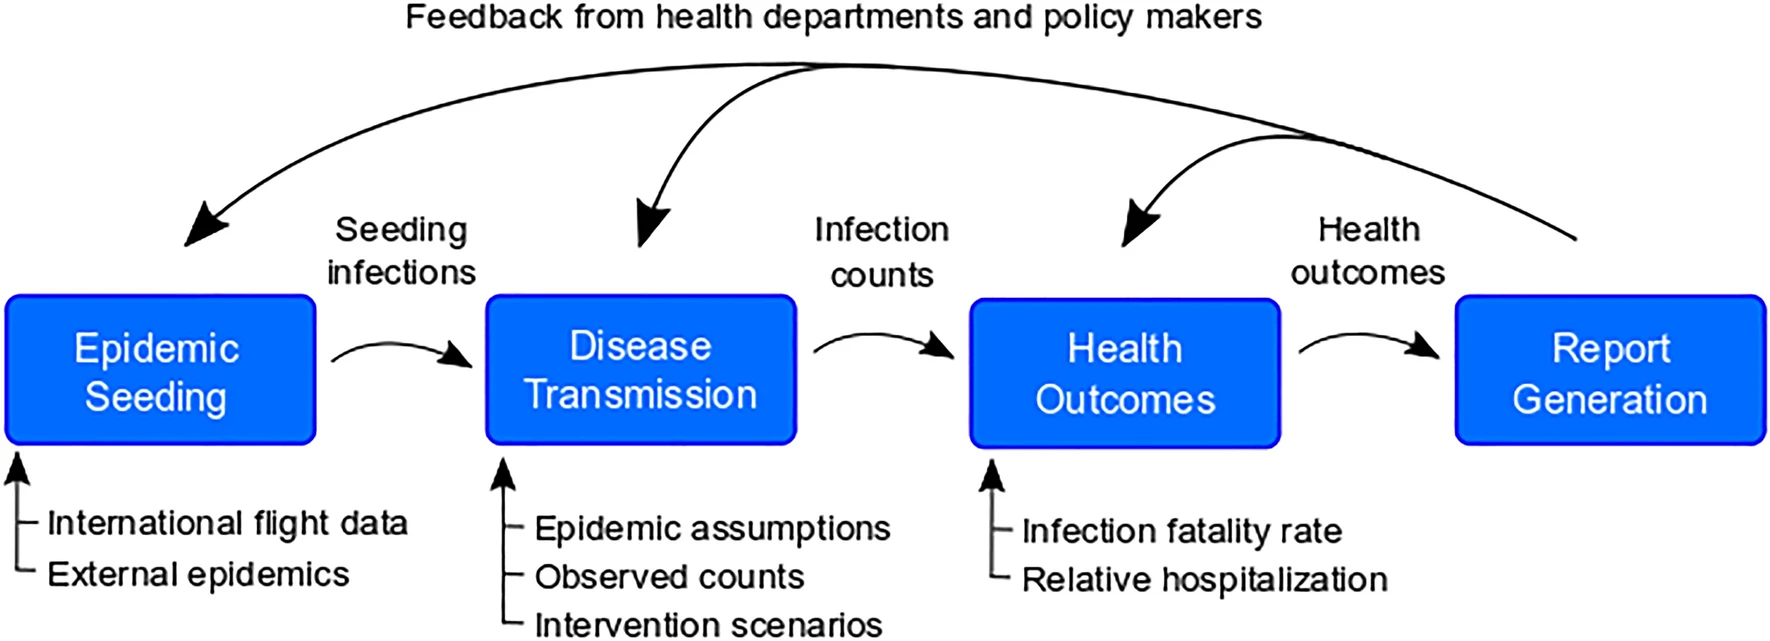
\includegraphics[width = .8\textwidth]{fig_pipeline/fig1a}
    \caption[Overview of the pipeline.]{Overview of the pipeline. The pipeline has four modules, each with specific inputs that can be specified by the user. First, it identified when and in which model locations epidemics are seeded using an air importation model or confirmed case data. Second, the epidemic seeding events are used to initiate the disease transmission model, which is informed by our epidemiological assumptions and intervention scenarios. The disease transmission model produces daily incident infection counts and infection prevalence. Next, health outcomes like hospitalizations and ICU admissions are calculated from these infection counts according to assumptions about health outcome risks and infection fatality ratios. Finally, these health outcomes may be summarized using templates and functions from the report generation component of the pipeline.}
    \label{fig:pipeline-modules}
\end{figure*}


These modular components of the pipeline fit together because each is composed of multiple pieces: an input format, an output format, one or more code libraries (where applicable), and a runner script. The standardized input and output formats ensure that components may be switched out according to user preference without impacting other phases. The “library” generally contains the core functions for a pipeline component. The script liaises between the user-defined configuration and the library by choosing which library to use and converting the input format to a format used by the library. 

The pipeline runs these components in sequence, according to the specifications outlined in a configuration file. This makes it easy to add or modify a component. To add a component, its input format is specified, and incorporate its dependencies. To modify the implementation of a component, functions in the library and function calls in the runner script are added or modified. When appropriate, entire components may be substituted with data from outside of the pipeline, provided that the data meet the input formats required by the next pipeline phase.

\subsection{Module 1: Epidemic seeding and initialization.} 

“Epidemic seeding” refers to how the disease transmission module is initialized with infected individuals. A seeding module must produce one of more seeding files that specifies an added number of incident cases occurring due to “seeding” at particular dates and locations. The pipeline currently contains two epidemic seeding options: (1) seeding according to first case appearance in data, and (2) seeding according to an air travel importation model. 

\paragraph{Seeding according to earliest identified cases.} This seeding option enables users to seed the model according to COVID-19 case data. It currently supports user-supplied data and downloads from two commonly used public sources, the Johns Hopkins University Center for Systems Science and Engineering (JHU-CSSE) COVID-19 Dashboard\cite{Dong:InteractiveWebbasedDashboard:2020} and USAFacts, a database that collates data from US state health departments\cite{USAFacts:USCOVID19Cases}. Drawing from the user-specified data source, this option identifies the first five days that cases were reported in each modeled location. It is assumed that confirmed cases were infected a user-specified number of days prior to when they were reported, and that there is a user-specified ratio of infections to confirmed cases. Seed infections are, hence, created in each modeled location on the estimated days of infection for the first 5 days with reported cases; they are drawn stochastically from a Poisson distribution where the mean is the product of the number of reported cases and the user-specified ratio. 

To facilitate the generation of the seeding file for US settings, the \verb|R/scripts/create_seeding.R| script is provided, which pulls data directly from USAFacts. 

\paragraph{Seeding according to an air importation model.} A previously published model of measles importation was adapted to model the rate of COVID-19 importation to specific locations due to air travel\cite{Truelove:EpidemicsAirTravel:2020}. This seeding option, available in the Github repository “\url{HopkinsIDD/covidImportation}”\cite{Truelove:HopkinsIDDCovidImportationInitial:2020}, uses complete itinerary (origin to final destination) air travel volume data from OAG\cite{OAG:FlightDataOAG} for all airports in the world, source location populations, and source location incidence data, to inform a model with which absolute counts of importation are estimated on a daily basis into airports\shortcite{Truelove:HopkinsIDDCovidImportationInitial:2020}. 

Geographic areas surrounding airports are classified spatially into “airport catchment areas” with a Voronoi tessellation of space in reference to the latitude and longitude coordinates of the airport\cite{Balcan:ModelingSpatialSpread:2010}. When there are multiple airports within close proximity, the user may specify a threshold distance under which airports may be grouped into a single cluster that is defined by its centroid. The probability of importation is assigned to each intersection of a Voronoi tile and an administrative unit boundary. This probability is calculated as the proportion of the airport catchment area population that lives in that intersection, assuming that population is distributed evenly by area. All air importations on a given day are then aggregated to the administrative unit level and seeded into the epidemic model as newly infected individuals.

\subsection{Module 2: Transmission model and intervention scenarios.}
The disease transmission module takes in seeding information and produces an epidemic model output file that contains, at minimum for subsequent module compatibility, daily counts of incident infections, indexed to their time of symptom onset. The currently implemented default transmission module comprises a metapopulation model with stochastic Susceptible-Exposed-Infected-Recovered (SEIR) disease dynamics.

\paragraph{Disease dynamics} The core model is a modified SEIR compartmental model where the time in the “Infected” compartment follows an Erlang distribution (i.e., the infected compartment is split into k compartments) to produce more realistic infectious periods where the chance of recovery depends on the time since infection\cite{Yan:QuantitativeMethodsInvestigating:2019}, and a coefficient ($\alpha$) can be set to help the model approximate non-homogeneous mixing between susceptible and infected individuals and non-exponential growth\cite{Finkenstadt:StochasticModelExtinction:2002}. Currently k is fixed at three compartments. Transition of individuals between disease compartments is simulated stochastically with binomial random draws:
\marginnote{The model for SARS-CoV-2 transmission is entirely configurable to any compartment model following an arbitrary transition graph, allowing for multi-strain, age-stratified or vaccination models.}

{\begin{eqnarray}
N_{S \to E} (t) &=& \text{Binom}\left(S, 1 - \exp \left(- \Delta t \cdot \text{FOI}(t) \right)\right) \\
N_{E \to I^{( 1)}} (t) &=& \text{Binom}\left(E, 1 - \exp \left(- \Delta t \cdot \sigma  \right) \right) \\
N_{I^{( 1 )} \to I^{( 2)}} (t) &=& \text{Binom}\left(I^{( 1)}, 1 - \exp \left(- \Delta t \cdot \gamma' \right) \right) \\
N_{I^{(2)} \to I^{(3)}} (t) &=& \text{Binom}\left(I^{(2)}, 1 - \exp \left(- \Delta t \cdot \gamma' \right) \right) \\
N_{I^{(3)} \to R} (t) &=& \text{Binom}\left(I^{(3)}, 1 - \exp \left(- \Delta t \cdot \gamma' \right) \right) \\
\gamma' &=& \gamma \cdot k
\end{eqnarray}

where $S$, $E$, $I^{\left(1\right)}$, $I^{\left(2\right)}$, $I^{\left(3\right)}$, and $R$ represent the number of individuals in those respective compartments, FOI(t) is the force of infection from the infected population on the susceptible population, $\frac{1}{\sigma}$ is the latent period, $\frac{1}{\gamma}$ is the infectious period, and $k$ is the number of $I$ compartments. The force of infection, which modulates transition of individuals from the $S$ to $E$ compartments:

\begin{eqnarray}
I(t) &=& \sum\limits_{{j = 1}}^{k} I^{( j)} \\
\text{FOI}(t) &=&\beta \cdot \frac{I{(t)}^{\alpha}}{H} \\
H &=& S(t)+E(t)+\sum_{j=1}^{k} I^{\left(j\right)}(t)+R(t) \\
\beta(t) &=& R_{0}\cdot\gamma
\end{eqnarray}
where $H$ is the total population, $\beta$ is the daily transmission probability as defined by $R_0$ and the infectious period, and $\alpha$ is the mixing coefficient.


\paragraph{Metapopulation dynamics}
The model is capable of simulating disease spread in multiple locations jointly according to assumptions about population mobility between individual model locations (e.g., administrative units). The SEIR disease dynamics described above are simulated in each model location with a modification to the force of infection term that accounts for this impact of mobility on disease spread.

The force of infection in a given location i is calculated from a combination of local infections and infections in locations that are connected to it according to the mobility matrix, as follows:
\begin{fullwidth}
\begin{equation}
FOI_i = \left(1 - \sum_{j\neq i} p_{away} \frac{M_{i,j}}{H_i} \right) \cdot \beta_i(t) \frac{(I_1^{i} + I_2^{i} + I_3^{i})^\alpha}{H_i} +  \sum_{j \neq i} \left(p_{away} \frac{M_{i,j}}{H_i} \cdot \beta_j(t) \frac{(I_1^j + I_2^j + I_3^j)^\alpha}{H_j} \right)
\end{equation}
\end{fullwidth}

with $p_{away}$ the percent of the time individuals that move spend away; $p_{away} \approx 0.5$ in the case of commuting. $H_i$ is the population of node $i$. Then, the transition is:

\begin{equation}
N_{S_i \longrightarrow I_1^{i}}(t) = \text{Binom}(S^i, 1 - \exp(-\Delta t \cdot FOI_i))
\end{equation}
where M is a mobility matrix such that $M_{i,j}$ represents the daily movement of individuals (e.g., commuting) from origin $i$ to destination $j$, $p_a$ is the proportion of time that moving individuals spend away, and $H_i$ is the population of node $i$. The transition of individuals between disease compartments may be modified to index by location $i$, for example:

\begin{equation}
N_{S_i \to E_i} (t) = \text{Binom}\left(S_i ,1 - \exp \left(- \Delta t \cdot\text{FOI}_{i}(t) \right) \right)
\end{equation}
Users may provide a symmetric or asymmetric wide-form mobility matrix for all model locations or a long-form sparse mobility matrix that indicates only pairs of model locations with connectivity.
\begin{figure*}[!htb]%[width = .7\textwidth]
    \centering
    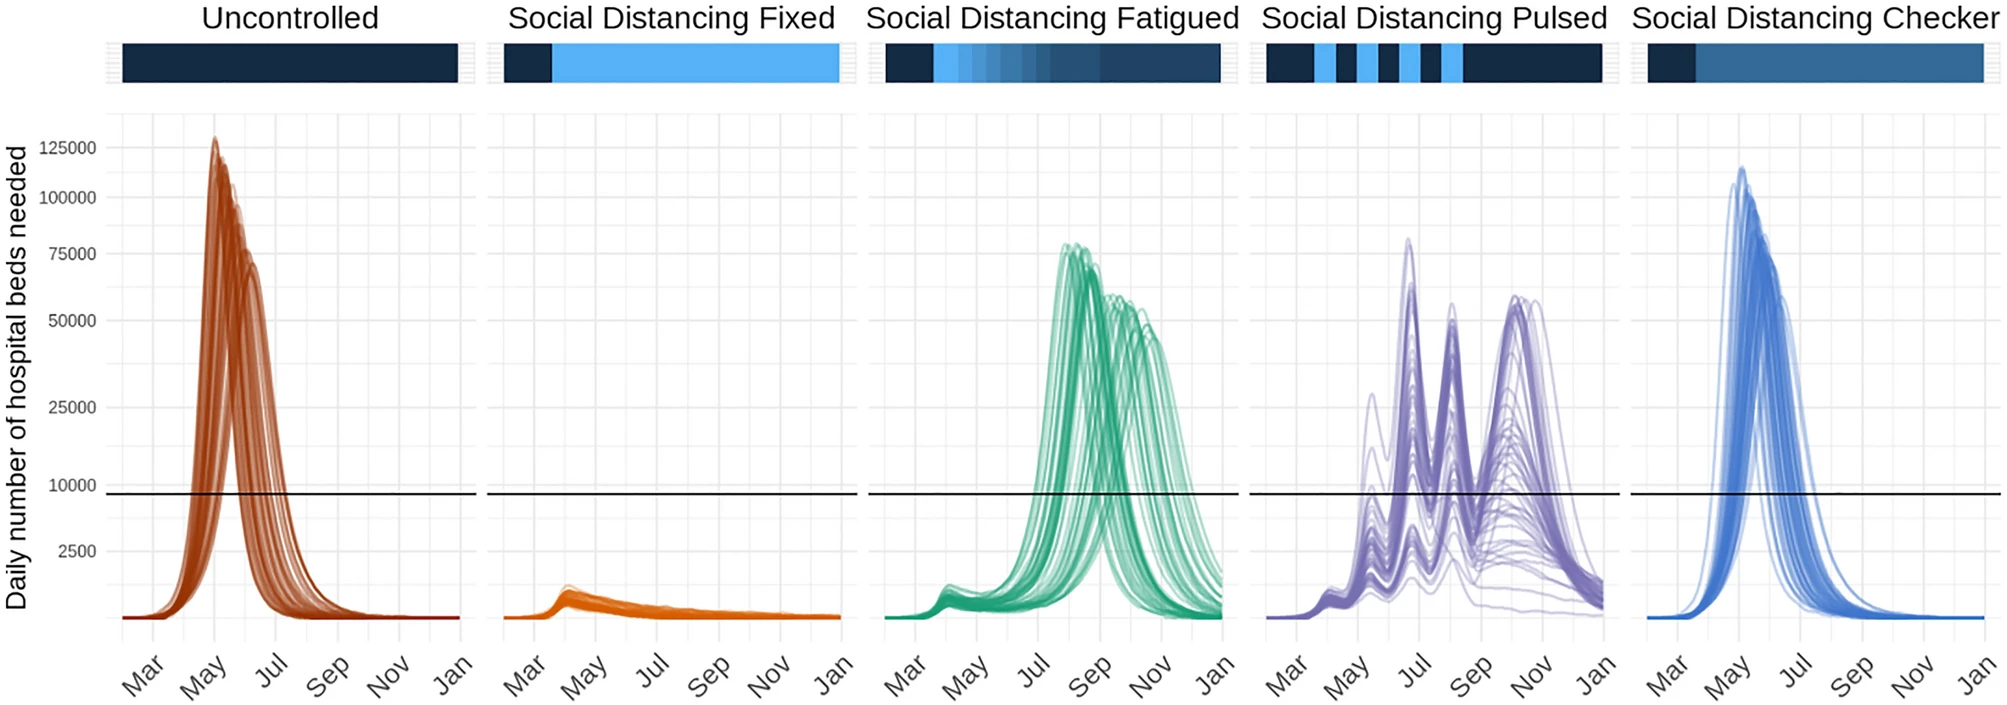
\includegraphics{fig_pipeline/fig2a}
    \caption[Time series of daily number of hospital beds needed across scenarios.]{Time series of daily number of hospital beds needed across five possible intervention scenarios in a fictional location with nine counties. Lines represent results from 50 stochastic model simulations. Horizontal black lines represent the total hospital bed capacity in the fictional location, assumed to be n = 8661 (3 beds per 1000 population). The colored horizontal bars along the top visualize the effectiveness of interventions at a given time point along a dark blue to light blue spectrum; dark blue indicates a period with no reductions to transmission, while light blue indicates a period with more restrictive action (i.e., low transmissibility). In the fifth scenario, “Social Distancing Checker,” only three of nine counties implement any non-pharmaceutical interventions, thus differentiating it from “Social Distancing Fixed”.}
    \label{fig:pipeline-seir}
\end{figure*}


\paragraph{Application of transmission modifiers}
In the absence of vaccines and other preventive treatments, non-pharmaceutical interventions, such as school closures, social distancing, stay-at-home directives, and testing and isolation are critical strategies for reducing disease transmission. Disease transmission may also change across space or time as the result of exogenous factors like seasonality or spatial heterogeneity in contact patterns. The model enables users to specify changes to the basic reproductive number ($R_0$) and the inverse of the infectious period ($\gamma$), for pre-specified periods of time to all or subsets of model locations independently. These interventions or exogenous changes can be implemented with fixed or distributional effectiveness. In addition, users may specify a rate of fatiguing effectiveness (e.g., declining adherence to a policy) over a certain number of days. This format enables flexibility in scenario planning; for instance, the model can be used to examine the effects of chaining multiple interventions together over time (e.g., school closure then stay-at-home), gradual declining adherence of the population to an intervention, switching interventions on and off over time, spatially heterogeneous interventions, or innate spatiotemporal heterogeneities (Fig. 2).

Transmission modifiers like non-pharmaceutical interventions or other exogenous factors modulate the daily transmission term below:
\begin{equation}
\beta _i'(t)=\left(1-r_i(t)\right)\cdot \beta_i (t)
\end{equation}

where $\beta_i'(t)$ is the daily transmission rate after accounting for transmission modifier $r_i(t)$ at the specified location $i$ at time $t$. When transmission modifiers are in effect $\beta_i'(t)$ replaces $\beta_i(t)$ in the force of infection term $\text{FOI}_i(t)$.


The specification of transmission modifiers is completely user-specified. A set of common non-pharmaceutical intervention scenarios that can be applied for user-specified dates and locations are included (Table S1), which have been compiled according to our review of the literature on the potential impact of non-pharmaceutical interventions on respiratory virus transmission.

Note that several effects at the same time in the same place have a compounded effect on transmission of reductions. The effect of the $k$ intervention in place at time $t$ and node $i$ is:
\begin{equation}
	\beta_i'(t) =  \beta_i(t) \cdot  \prod_k \left(1-r_k(t) \right), \label{eq:npi_comp}
\end{equation}
but the compounding effect may be choosen to be additive (\ie usefull for vaccination rate) instead of multiplicative.

\subsection{Module 3: Calculation of health outcomes}
This pipeline module translates outputs from the transmission model into health outcomes such as hospitalizations and deaths. It takes in counts of daily incident infections and produces daily counts for specific health outcomes at appropriate time delays.

The current default implementation produces hospital and intensive care unit (ICU) admissions, current hospital and ICU occupancy, ventilators needs, and number of deaths. Our modeling of health outcomes assumes that there is some transition probability from infection to death, infection to hospitalization, hospitalization to ICU admission, and ICU admission to ventilator use. In our modeling of health outcomes, is considered the probability of its occurrence (e.g., probability that infections are hospitalized), the time delay relative to its disease course (e.g., time between hospital admission and ICU admission), and where applicable, the duration in a given state (e.g., how long a patient remains ventilated).

For settings where hospitalization, ICU admission, and ventilator use is infrequent, it may be more appropriate to think of these health outcome projections as different levels of disease severity.

The user may specify health outcome probabilities and delays, conditional on the flows described above. For use as default values, tables of parameter values derived from a literature review of COVID-19 health outcomes are provided.

The pipeline currently contains two versions of this module with different approaches to the specification of health outcome risks: (1) unadjusted, uniform risk and (2) location-specific risks, adjusted by key demographic or health factors in each location.

\paragraph{Unadjusted, population-wide health outcome risks}
This option generates health outcome estimates with unadjusted risk across all locations, assuming fixed values for all health outcome probabilities, delays and durations.

It is assumed that the number of infections admitted to the hospital is a draw from the Binomial distribution, lagged by a fixed time from symptom onset to hospital admission:
\begin{equation}
n_{t_\text{inf} + t_\text{inf} \to \text{hosp}}^{hosp} \sim Binom\left(n_{t_\text{inf}}^\text{inf}, p_{\text{hosp}| \text{inf}} \right)
\end{equation}
where $n^\text{hosp}$ is the number of hospital admissions, $n^\text{inf}$ is the number of infections, $t_\text{inf}$ is the time of infection, $t_{\text{inf} \to \text{hosp}}$ is the mean time delay between infection and hospital admission, and $p_\text{hosp|inf}$ is the probability of hospitalization given infection (Table 1).

\begin{table*}[t]
\caption[Health outcome risk parameters.]{Health outcome risk parameters.}
\label{tab:vdparams}
\centering
\begin{tabular}{ll}
\toprule
 Column name (notation, as appropriate) & Description\\
\midrule
\verb|p_hosp_inf| ($p_{\text{hosp|inf}}$)	& Probability of hospitalization among infected individuals\\
\verb|p_icu_hosp| ($p_{\text{icu|hosp}}$)	&Probability of ICU admission among hospitalized individuals\\
\verb|p_vent_icu| ($p_{\text{vent|icu}}$) &	Probability of ventilation among individuals in the ICU\\
\verb|p_death_inf| ($p_{\text{death|inf}}$)&	Probability of death among infected individuals\\
\verb|rr_hosp_inf|	& Relative risk of hospitalization (given infection) relative to the average across all geoids\\
\verb|rr_death_inf| & Relative risk of death (given infection) relative to the average across all geoids\\
\bottomrule
\end{tabular}
\end{table*}

A similar assumptions is made for the transitions between other outcomes (hospitalization admission to ICU admission, ICU admission to ventilator use, infection to death):
\begin{eqnarray}
n_{t_\text{hosp} + t_\text{hosp}\to \text{icu}}^\text{icu} &\sim & Binom\left(n_{t_\text{hosp}}^\text{hosp} , p_{\text{icu}| \text{hosp}} \right)\\
n_{t_\text{icu} + t_\text{icu} \to \text{vent}}^\text{vent} &\sim & Binom\left(n_{t_\text{icu}}^\text{icu}, p_{\text{vent} | \text{icu}} \right) \\
n_{t_\text{inf} + t_\text{inf} \to \text{death}}^\text{death} &\sim & Binom\left(n_{t_\text{inf}}^\text{inf}, p_{\text{death}| \text{inf}}  \right)
\end{eqnarray}
The number of patients currently hospitalized, admitted to ICU, and ventilated are generated from the incident number of events and fixed (non-distributional) user-defined durations for each event.

As information about the death and hospitalization rates were scarce early on in the pandemic, decision makers wanted to consider how things would unfold over different scenarios of health burden. To facilitate these needs, our pipeline separates hospitalization and death rates from the other outcomes, and allows users to consider multiple scenarios for different rates.

\paragraph{Location-specific health outcome risks}
The severity of disease from SARS-CoV-2 infection can vary greatly between locations due to difference between populations; individuals that are older, with limited access to health care, or with certain pre-existing health conditions are at greater risk for severe disease and death. For this reason, the hospitalization module also supports the specification of location-specific relative risks, which can be used, for example, to standardize hospitalization and mortality rates according to the age distribution of the population. Users may provide a wide format data file with standardized variable names for the transition probabilities and relative risks (columns) by geoid (rows). These transition probabilities are conditional on previous states (e.g., probability of hospitalization given infection is named \verb|p_hosp_inf|). The probability of hospitalization and death given infection are specified as relative values compared to population-wide averages specified in the configuration file. The location-specific standardizations apply only to the health outcomes, making a critical assumption that all individuals are at equal risk of infection.

While location-specific data is not required to differ for all health outcome transition probabilities (i.e., some probabilities can be constant across all locations), the location-specific file should include the variables described in Table 1 and population-wide average values for the probability of hospitalization (\verb|p_hosp_inf|) and death (\verb|p_death_inf|) given infection.

To facilitate construction of such files a companion package, covidSeverity, is provided. It produces location-specific relative death and hospitalization rates based on the age distribution of the local population\cite{Lauer:HopkinsIDDCovidSeverityInitial:2020}. The package generates these outputs for US counties based on data from the US Census Bureau, and  this is provided as a model input file as part of the main pipeline implementation (see \verb|COVIDScenarioPipeline/sample_data/geoid-params.csv|). The package also includes built-in functionality to pull data from WorldPop\sidenote{\url{worldpop.org}} and generate adjustments for any location of interest\shortcite{Lauer:HopkinsIDDCovidSeverityInitial:2020}.

The covidSeverity package applies a logistic generalized additive model (GAM) with a penalized cubic spline for age and random effect for age-specific estimates of risk of each health outcome from the literature, thus producing estimates of risk for 10-year, aggregated age categories. These age-specific estimates are then applied to the population age distribution in a given location.

The epidemic transmission model, the intervention module and the outcome calculation are implemented in python, just-in-time compiled to machine code using Numba\cite{Lam:NumbaLLVMbasedPython:2015}. 

\sidenote{Since this description, the team working on the pipeline has brought many improvements, both computational and conceptual, that have enabled the pipeline to remain useful in 2021.}

\subsection{Module 4: Summarization of model outputs}
This component of the pipeline provides wrapper functions for the lightweight summarization of model outputs into quantiles, plotting functions for common figures, and R Markdown templates to facilitate the rapid generation of technical reports. This module is available in the R package report.generation in the Github repository “\verb|HopkinsIDD/COVIDScenarioPipeline|.”

Two key functions that read and process individual transmission (\verb|load_scenario_sims_filtered|) and health outcome (\verb|load_hosp_sims_filtered|) model output files are provided. In managing individual files with these functions, the processing time and memory load is reduced. Both of these functions take processing functions as arguments, thus enabling aggregation and filtering to occur at the level of individual files.

The package contains technical report R Markdown templates for US states, US counties, and individual countries, a diagnostic report template called “\verb|sanity_check_report|”, and a template that is maintained solely for integration testing. When report.generation is installed and loaded, the templates become available to the user. Many parameters are drawn from the configuration file automatically and pre-written R Markdown chunks about the module options and methods can be referenced within the package.

Common figures include summary tables and time courses for estimated health outcomes under different interventions, maps that portray cumulative cases at the county level, comparisons between model estimates and observed cases and deaths, and visualizations for when ICU and ventilator capacity for each county is exceeded. The vignette below walks through example report outputs in more detail and a template-generated report example is provided in the “Supplementary Material” (Example Report).

\subsection{Model specification}
All components and settings for simulations from the COVID Scenario Pipeline model are specified in an easily-modifiable YAML configuration file. Different options are described in detail in the \textsc{Results} and an example of the complete set of configuration options is provided in the “Supplementary Material”.

\subsection{Model access and use}
The project is open-source under the GNU General Public License v3.0 license, and code is available at \url{github.com/HopkinsIDD/COVIDScenarioPipeline}. The master branch of this repository consists of a Python package “SEIR” and two R packages “hospitalization” and “report.generation,” which correspond to the second, third, and fourth modules of the model pipeline (\url{zenodo.org/badge/latestdoi/245866576}). Air importation-based seeding is implemented in the covidImportation package (\url{github.com/HopkinsIDD/covidImportation}), while seeding according to the earliest identified cases is performed in scripts within the \url{HopkinsIDD/COVIDScenarioPipeline} repository.

\section{Results: scenario modeling vignette}
Here is presented a vignette with 50 model simulations in a fictional setting (Location X) with nine counties (named A through I) in demonstrative intervention scenarios from January 31 to December 31, 2020. In this vignette, a walk through is offered on how to set up and run the pipeline, demonstrate some of the spatial and temporal features for modeling non-pharmaceutical interventions, and display some of the plotting functions useful for summarizing the model output.

To run the model, users will require the functionality of the “\verb|HopkinsIDD/COVIDScenarioPipeline|” repository and a second GitHub repository specific to their model location. A template for such a spatial repository may be found at “\verb|HopkinsIDD/COVID19_Minimal|” (\url{github.com/HopkinsIDD/COVID19_Minimal}), and complete details on downloading and running the model are available in the template’s wiki at \url{github.com/HopkinsIDD/COVID19_Minimal/} wiki.

Once a working environment is setup, the next step is to create a configuration file to describe the model specifications. A skeleton configuration file is included in the \verb|COVID19_Minimal| template, and the full configuration file accompanying the results of this vignette is in the “Supplementary Material”.

First, the broad parameters of the run, such as the date range covered and the number of simulations to run are provided (see first section in “Supplementary Material”, Example YAML Configuration File).

Next the spatial setup information identifying the location of files containing geographic data and the geographic targets for modeling are described. The \verb|spatial_setup| section of the configuration file identifies a geographical data (geodata) file that contains the population data for each county or administrative subunit in the location(s) of interest and a mobility matrix file that contains the daily trip counts for each pair of counties. Users may employ the R scripts “\verb|build_US_setup.R|” or “\verb|build_nonUS_setup.R|,” which are provided with the repository, to generate compatible geodata and mobility matrix files. For users modeling non-US settings, the Github repository “\url{COVID-19-Mobility-Data-Network/mobility}” can be used to fit real-time or sparse travel data with mobility models in order to generate similarly compatible mobility matrixes\cite{Giles:COVID19MobilityDataNetworkMobilityV0:2020,Giles:MobilityPackageModeling}.

In situations with high cross-border mobility, it may be important to model a region larger than the location of interest in order to appropriately capture disease transmission risk in a given location. Here, Locations X, Y, and Z are modeled even though Location X is the sole location of interest:
FIG

The locations of the seeding files are then specified (see seeding section in “Supplementary Material”, Example YAML Configuration File), with a separate section to describe the air importation model parameters as appropriate (see importation in “Supplementary Material”, Example YAML Configuration File).

Next, the parameters that determine the course of the disease are choosen. The seir section of the configuration file defines parameters used in the SEIR disease transmission model, including the level of population mixing (where 1 is homogeneous mixing, and <1 is heterogeneous), the incubation period of the virus, the infectious period, and the baseline basic reproductive number R0. These values may be fixed or drawn randomly from a distribution, according to the configuration file:
FIG
Typically sigma and gamma are parameterized in our model with estimates of the range of the serial interval (SI) or generation time, such that
\begin{equation}
\text{SI}=\frac{1}{2}\left(\frac{1}{\gamma }\right)+\frac{1}{\sigma },
\end{equation}
which assumes that the average infection occurs halfway through an index case’s infectious period.

The next step is defining the modeled intervention scenarios. Here, five scenarios are considered in our vignette example: (1) a no intervention scenario (named Uncontrolled), in which R0 remains unchanged over the course of the outbreak; (2) social distancing measures with fixed effectiveness in place from March 19 to December 31 (\verb|SocialDistancing_fixed|); (3) social distancing measures with declining compliance, which were modeled as 10\% reductions in effectiveness every 2 weeks beginning March 19 (\verb|SocialDistancing_fatigued|); (4) social distancing measures following a 3-week on–off “pulsing” cycle from March 19 to August 12 (\verb|SocialDistancing_pulsed|); and (5) social distancing measures with spatial heterogeneity (\verb|SocialDistancing_checker|), where three of nine counties implement social distancing measures with fixed effectiveness from March 19 to December 31.

%\begin{mybox}{Initial parameters}
\marginnote{\textsc{Initial parameters}The serial interval represents which is the interval between two subsequent infections. For SARS-CoV-2, the serial interval was estimated to be in range $6.5-8.2$, from: \fullcite[][Table S4]{Bi:EpidemiologyTransmissionCOVID19:2020}. 

The basic reproductive number $R_0$ -- the number of newly infected caused by an infecteds in a fully susceptible population, has been estimated in the range 2 -- 3. From: \fullcite{Riou:PatternEarlyHumantohuman:2020}. This very early work also characterize $R_0$ and the dispersion of the number of secondary cases as important epidemic characteristic.
}

An intervention may be specified in a single block for all model locations, as in the case of the \verb|SocialDistancing_fixed| scenario, or for unique location identifiers (“geoids”) as in the \verb|SocialDistancing_checker| scenario:
FIG
Other intervention scenarios require multiple blocks to be stacked together, as in the case of the \verb|SocialDistancing_pulsed| scenario, shown in truncated form below: 

FIG

Then, the health outcome risk specifications are set up. In the hospitalization section of the configuration file, it is specified whether the model calculates health outcome risks with age-adjusted estimates, the average infection fatality ratios (IFR), and the time delays between different health outcomes. The time delays are modeled with lognormal distributions and parameterized with the log median and log standard deviation. For ease of use, a table of estimates found in the literature is provided in Table S2.

After the simulation runs complete, wrapid summaries of the results are produced using R Markdown templates provided by the report.generation package. The report section of the configuration file specifies scenario labels and colors, IFR scenario labels, and table display dates. These settings, along with other model parameters, can be loaded into a technical report template.

Here it is described how the \verb|state_report| template in the report.generation package can be used to display our model results as an example. The full template-generated report linked to this vignette is provided in the “Supplementary Material” (Example Report). First, the configuration file is loaded to pull in the model settings and file paths. Then, a number of predefined functions to load and plot the data are used.

For example, one standard report figure compares time series of the daily number of hospital beds needed across intervention scenarios (Fig. 2) using the \verb|load_hosp_geocombined_totals| and \verb|plot_ts_hosp_state_sample| functions from the report.generation package in order to load and plot the data. To plot variations of these figures, one only need to change which health outcome variable is specified in \verb|plot_ts_hosp_state_sample|.

While Fig. 2 displays aggregate results, our reports also provide location-specific risk and logistical outputs at the county- or administrative subunit-level. For example, the age-adjusted infection fatality ratios and risk of ICU admission among hospitalized infections for the modeled counties within the distribution of all counties in the United States are presented in Fig. 3A,B. Using the \verb|load_hosp_geounit_relative_to_threshold| and \verb|plot_needs_relative_to_threshold_heatmap| functions from report.generation, the potential need for beds in excess of health system capacity by model location is displayed in our reports (Fig. 3C). Values of the location-specific healthcare capacity, represented by the number of staffed hospital, acute care, or intensive care beds available and/or number of ventilators available, are user-defined; these can be based on assumptions of the average availability per person or input from data where available.

A map of model outputs makes it easier to visualize spatial and temporal heterogeneity in different intervention scenarios (Fig. 4). This functionality is provided in the \verb|load_cum_inf_geounit_dates| and \verb|plot_geounit_map| functions in the report.generation package.

Each report template is equipped to load static R Markdown reference chunks, which is pre-written and provided with the package. These chunks provide details on our methods, limitations, and key references, pulling in parameters from the configuration file as needed.

\section{Discussion}
The COVID scenario pipeline is presented as an open-source modeling framework that aims to balance epidemiological rigor with the flexibility and urgency required by public health policymaking. The modularity of our framework has enabled us to adapt our assumptions about COVID-19 epidemiology, transmission, and health outcome risks in response to emerging information and to different settings. The pipeline implementation of non-pharmaceutical interventions is highly adaptable for policymakers desiring to compare the impact of different potential scenarios.

\begin{figure}[!htb]%[width = .7\textwidth]
    \centering
    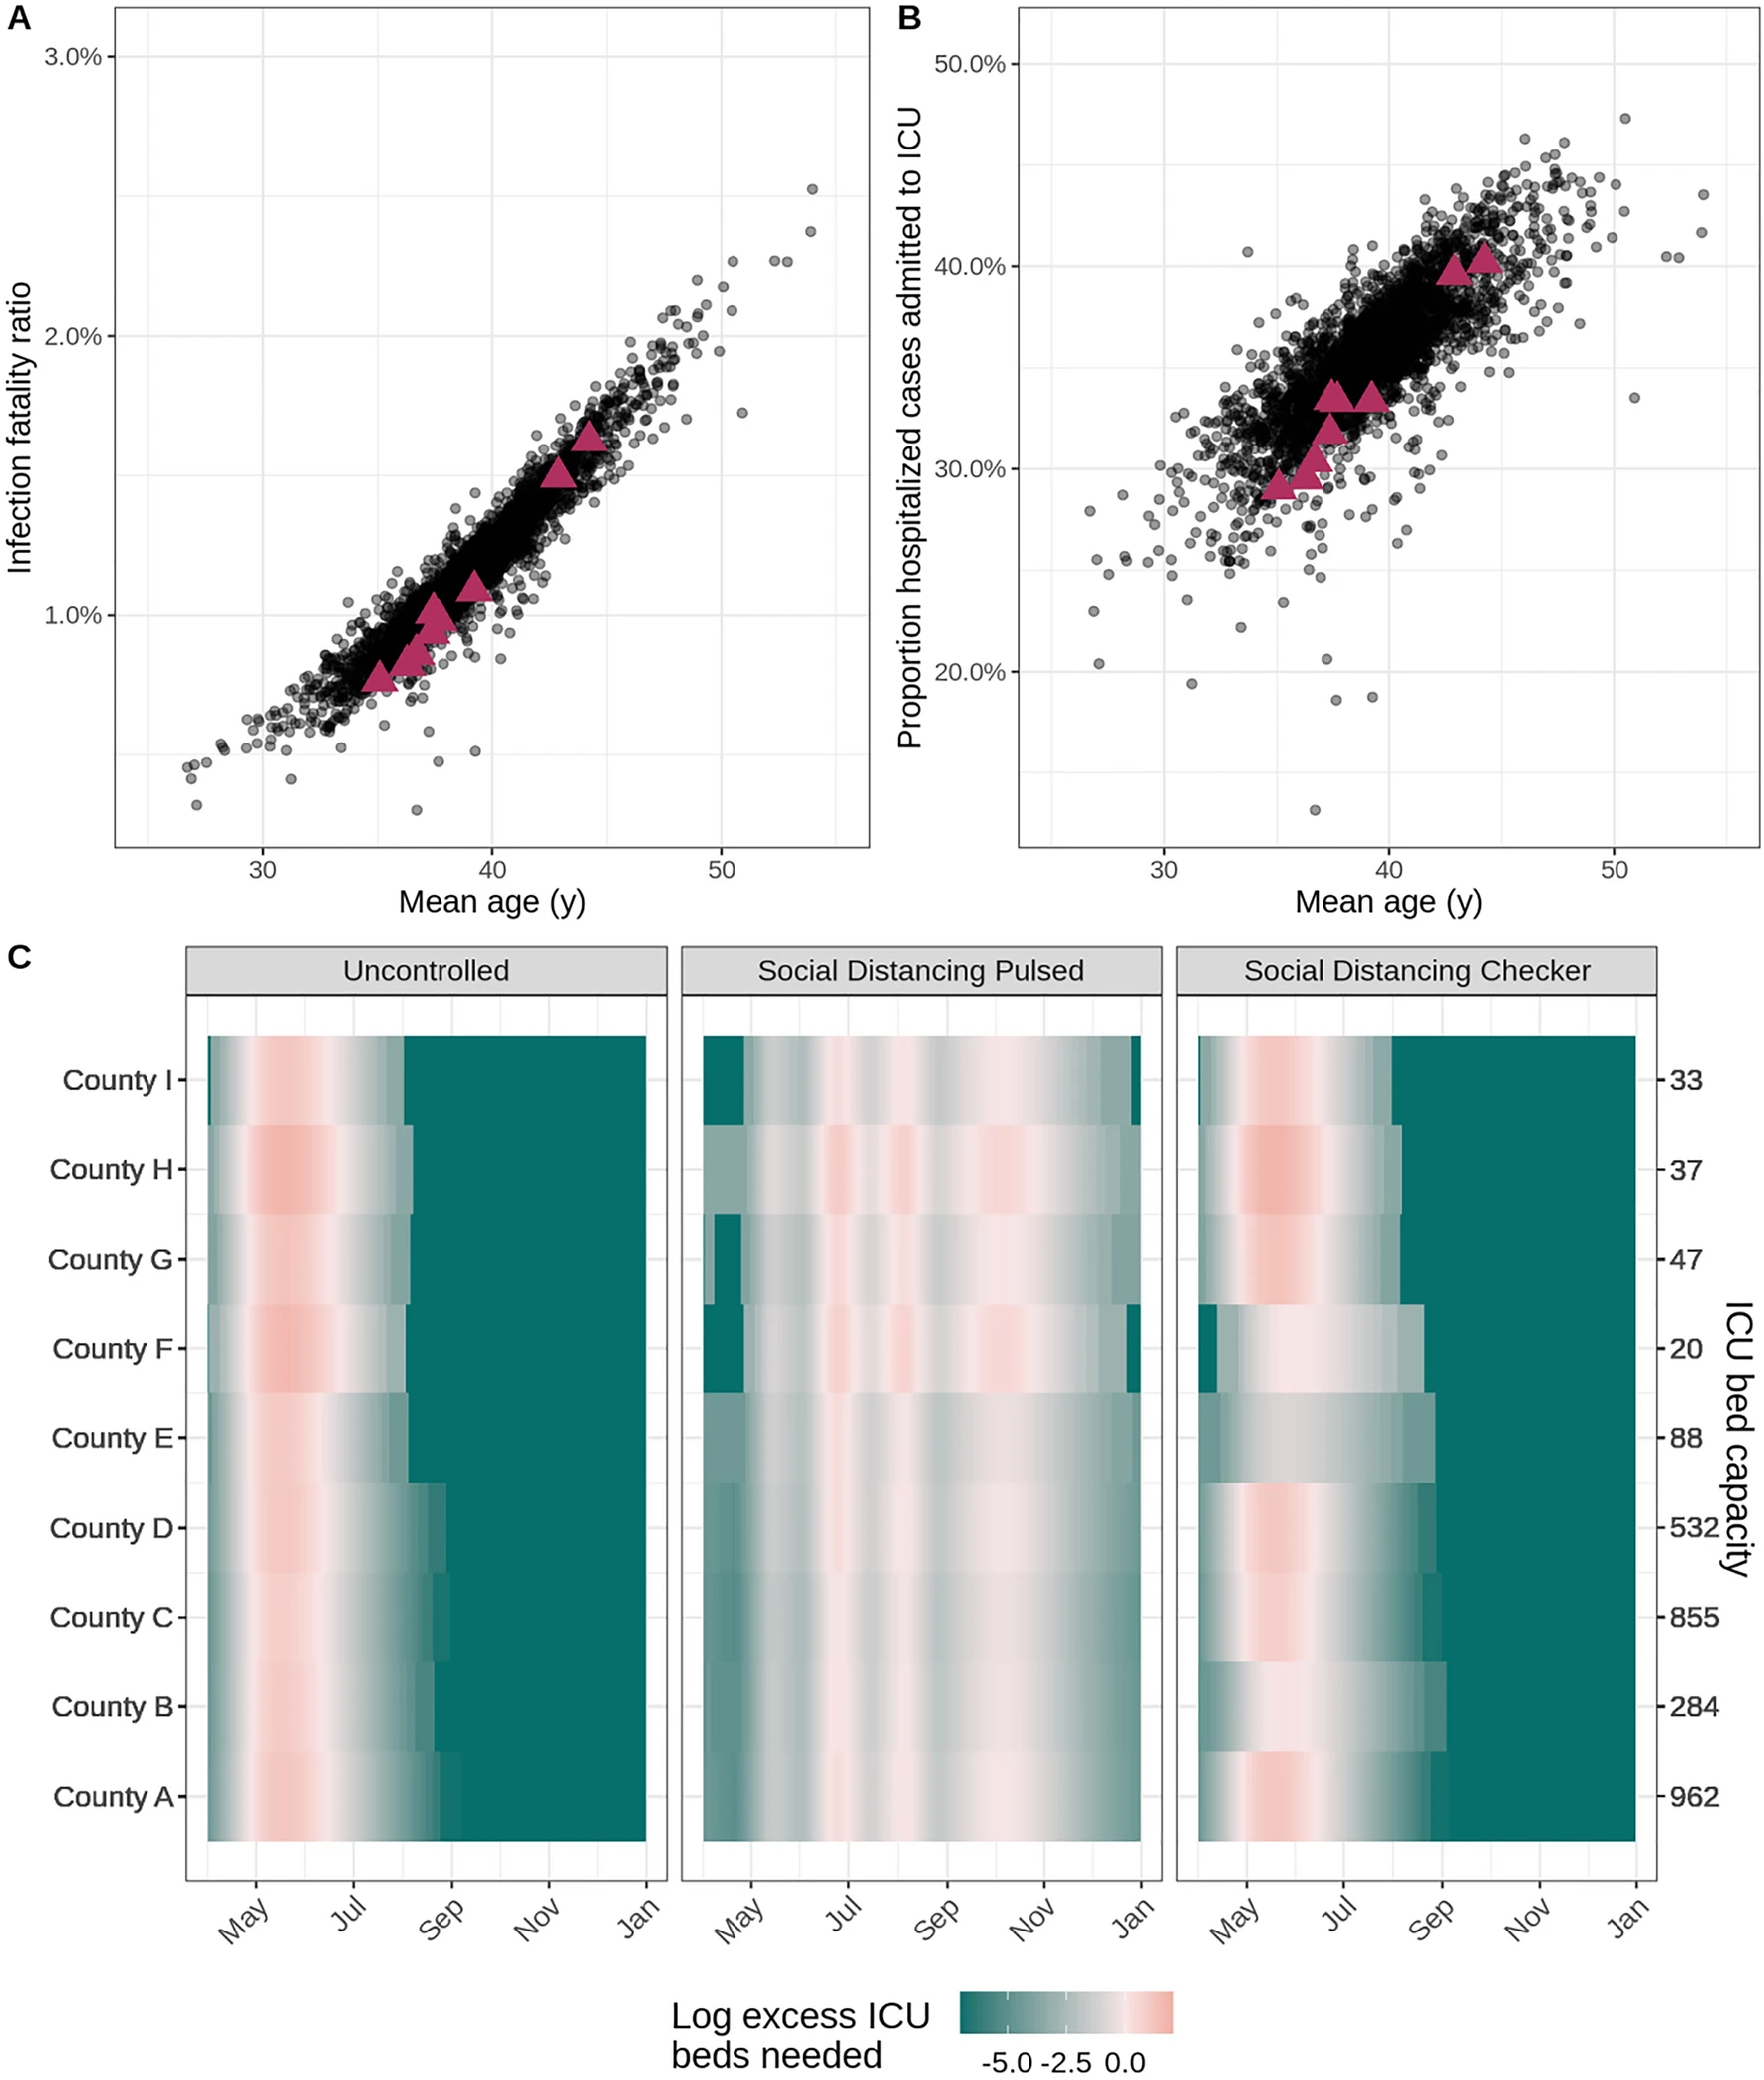
\includegraphics{fig_pipeline/fig3a}
    \caption[Health outcome risks and logistical needs for fictional counties.]{Health outcome risks and logistical needs for fictional counties. In the scatterplots, each point indicates (A) the age-adjusted infection fatality ratio and (B) risk of ICU admission given hospitalization by mean age for a county within the United States. Data for the nine fictional counties in our vignette is marked by magenta triangles. (C) The heat maps display county-level ICU bed needs, shaded according to the log ratio above or below the assumed ICU bed capacity (secondary y-axis) in each county (primary y-axis) for three example intervention scenarios (panels). The salmon pink shading indicates periods of time where ICU bed needs exceed capacity in the fictional counties.}
    \label{fig:pipeline-outcome}
\end{figure}

Throughout the course of the pandemic, the default settings of our pipeline have been adapted in response to the changing needs and questions of our collaborators. At the beginning of the pandemic, air importation seeding was a critical determinant of epidemic onset in specific locations. Now that cases of COVID-19 are present worldwide, the development shifted towards more empirical methods of epidemic seeding that better match trajectories of confirmed cases in specific locations as policy questions have shifted to more operational needs. As new data emerged, it was decided to move from calculating unadjusted health outcomes to health outcomes based on age-standardized risk of hospitalization, ICU admission, and death according to emerging case-study data.

As the COVID-19 pandemic continues, the plan is to continue to expand the scope of the COVID Scenario Pipeline to changing needs and questions. Future model releases will include a health outcomes model expansion that will enable a multiplicity of pathways to ICU occupancy, ventilator usage, and death. As questions have shifted to near-term operational needs, inference has been incorporated into our models, thus enabling the calibration of model trajectories to deaths and confirmed case counts, short-term forecast of health outcomes, and estimation of location-specific transmission parameters and NPI effectiveness.

While the pipeline’s generic structure means that different modules may be readily replaced, the current implementation of our model has several limitations with regard to the epidemiology of COVID-19. The disease transmission model does not explicitly incorporate age-specific contact or transmission rates or asymptomatic transmission, nor does it consider how factors like testing rates may lead to time-varying biases in reporting. Data to inform these factors was scarce when this model was initially developed, but these processes can change the dynamics displayed by scenario projections. Moreover, this model structure means that age-targeted interventions  (e.g., cocooning of high-risk age groups) cannot be modeled, nor are interventions targeting asymptomatic individuals (e.g., systematic age-specific testing) in a mechanistic manner. However, it is possible, and done is real settings, to adjust for these types of interventions through overall population-level reductions in disease transmission. Additionally, the current model cannot tune changes in population mobility or connectivity over time, although it is known that travel and movement restrictions played a role in changing the spread of COVID-19.

The health outcomes module also has several structural limitations; it assumes that only one progression in health outcome severity exists (infection to hospitalization to ICU to ventilator use), although it is known that many disease course progressions are possible. In addition, the delays and durations involved in our health outcomes progression are fixed in time for a given location, although stochastic variation may be incorporated across simulations..

Nevertheless, the modular approach taken is meant to allow for easy substitution of models with improvement in any of these areas while still taking advantage of other pipeline components. This feature has been leveraged throughout the course of the COVID-19 pandemic, and individual modules continue to develop. This flexibility does come at a cost, as the modular pipeline approach requires us to write and read files at the end and beginning of each phase, respectively. This procedure requires more disk space and input/output steps than other modeling approaches that can hold all of the necessary data in memory until a single output is produced at the end. Still, these slowdowns are not critically limiting; it has been possible to run 1000 county-level simulations of the United States in less than 10 min on a 96 core server.
\begin{figure}[!htb]%[width = .7\textwidth]
    \centering
    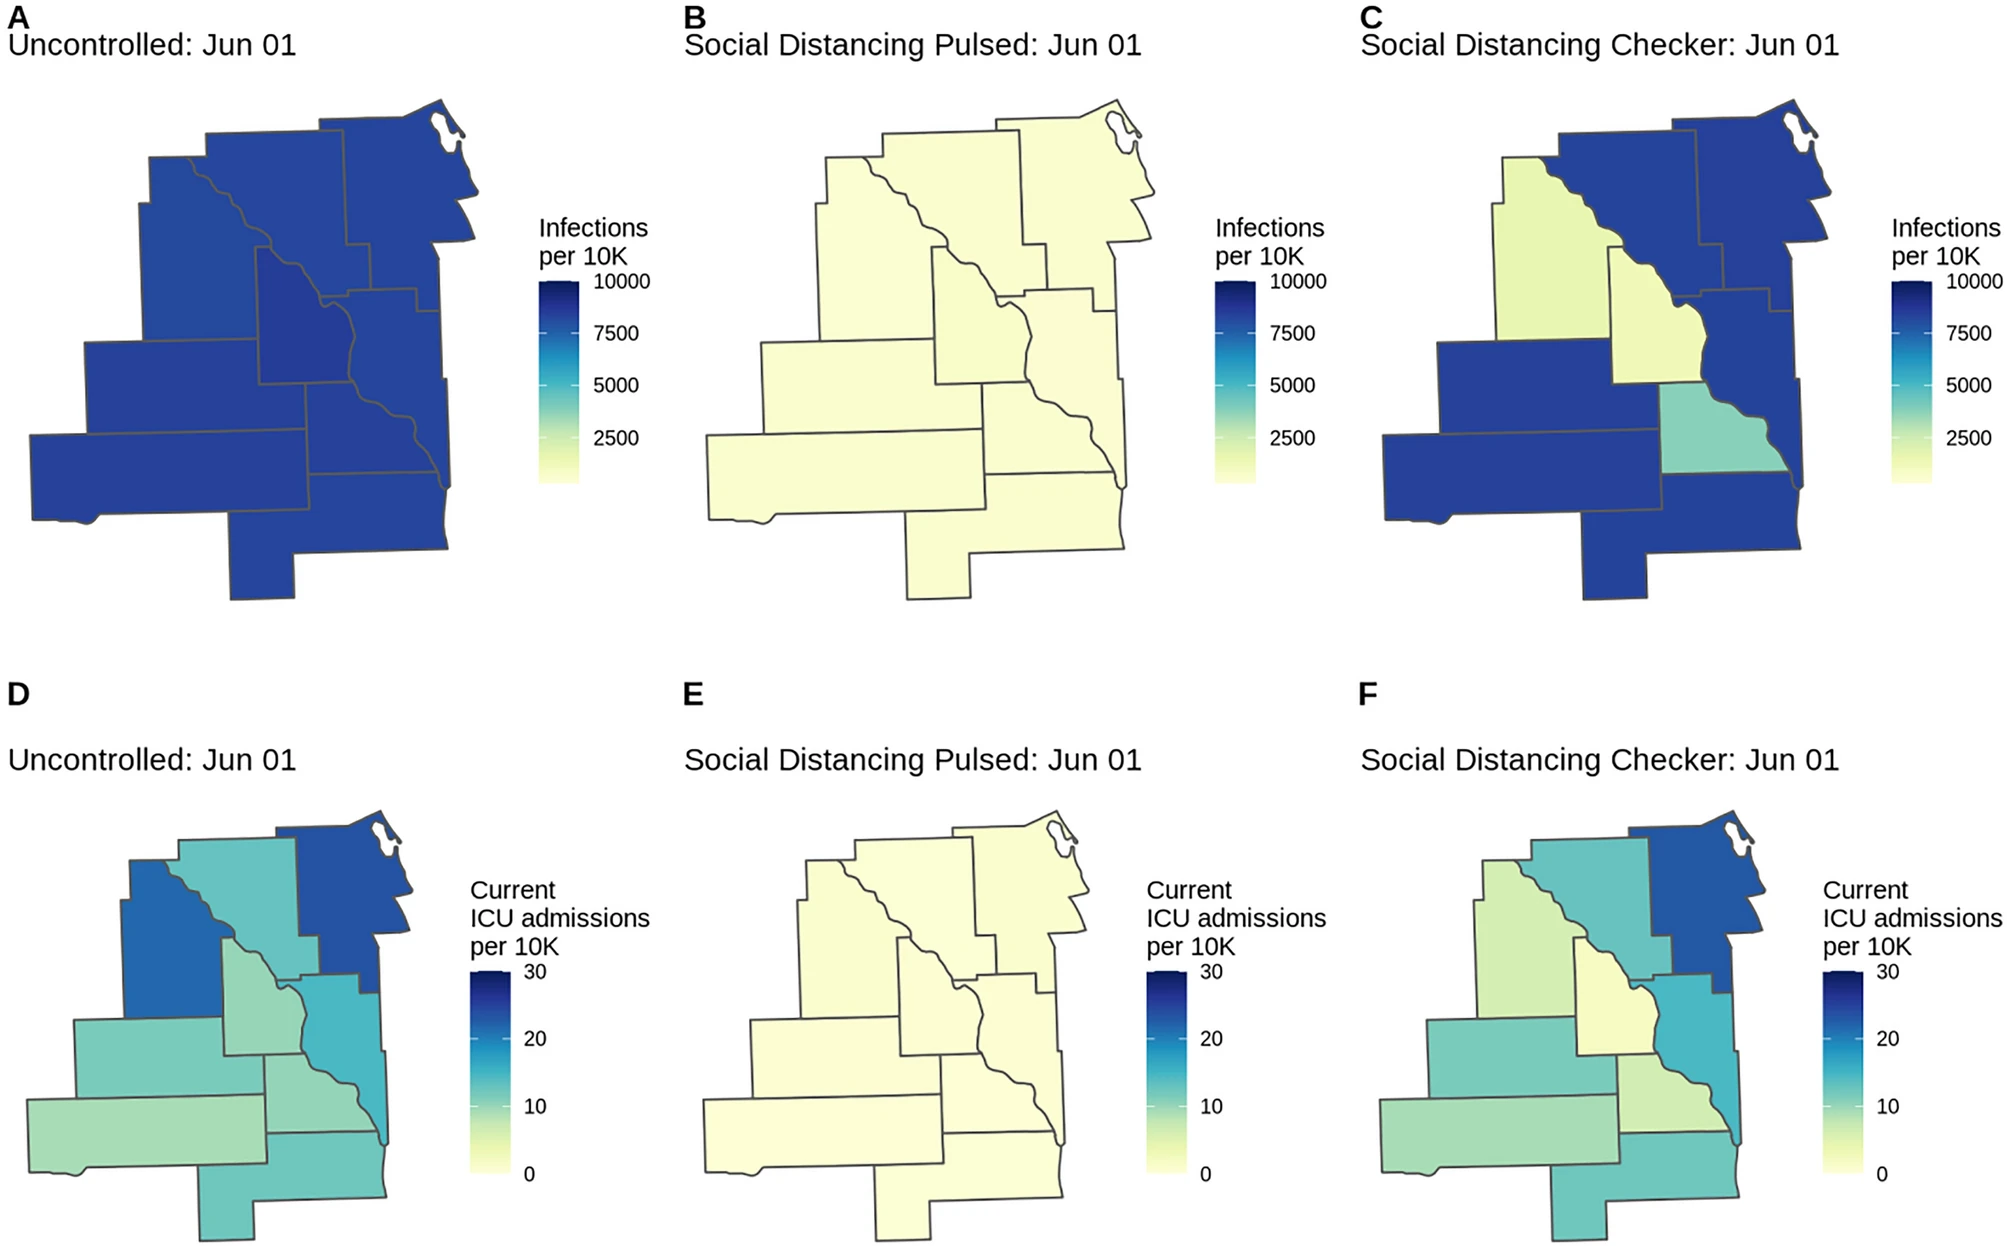
\includegraphics{fig_pipeline/fig4a}
    \caption[County-level COVID-19 risk for three scenarios.]{County-level COVID-19 risk for three scenarios (Uncontrolled, Pulsed, Checker) in the fictional Location X. Choropleths for model outcomes on June 1, 2020 of the (A–C) cumulative infection rate per 10,000 population and (D–F) number of patients currently admitted to the ICU per 10,000 population for the Uncontrolled, Social Distancing Pulsed, and Social Distancing Checker intervention scenarios. Countylevel variation in attack rates can arise from differences in risk of importation, mobility patterns connecting subdivisions, and differences in non-pharmaceutical interventions applied in each location. If location-specific health outcome risks are specified (as are age-standardized health outcome risks in this example), this may serve as another source of county-level variation.}
    \label{fig:pipeline-map}
\end{figure}

These limitations point to a broader need to consider the totality of evidence generated by epidemiologic models. While our approach is well-suited to answering policy questions about interventions, it is critical for policymakers to explore projections from multiple models in order to understand the range of possible trajectories and the sensitivity of results to different assumptions. Models that incorporate individual-level behaviors may be better for considering the impact of specific contact tracing strategies or location-specific measures like workplace occupancy or symptom screening policies that are not well captured in compartmental models such as ours\cite{Kucharski:EffectivenessIsolationTesting:2020,Firth:UsingRealworldNetwork:2020,Hinch:OpenABMCovid19AgentbasedModel:2020}. Other individual-based models are better suited for addressing heterogeneities due to differences in household or social structures\cite{Wilder:ModelingBetweenpopulationVariation:2020,Kerr:CovasimAgentbasedModel:2021}. Models incorporating real-time mobility data can best characterize the impact of movement-related restrictions\cite{Lai:EffectNonpharmaceuticalInterventions:2020} models with age-specific transmission may provide more detail on the impact of age-specific interventions like “cocooning”\cite{Duque:COVID19HowRelax:2020} or closing and opening schools\cite{Ferguson:ReportImpactNonpharmaceutical:2020}. Still other models are particularly suited to address questions about health systems burden and forecast operational needs\cite{Branas:FlatteningCurveIt:2020,LosAlamosNationalLaboratory:COVID19CasesDeaths,Weissman:LocallyInformedSimulation:2020} and to consider the economic impacts of transmission and interventions\cite{Acemoglu:OptimalTargetedLockdowns:2020,Silva:COVIDABSAgentbasedModel:2020}. Integrating knowledge from multiple models, where appropriate, with careful consideration of the assumptions and appropriate applications of each model, will strengthen response and preparedness\cite{Shea:HarnessingMultipleModels:2020}.


Our flexible modeling pipeline brings an important voice to this “conversation” of models, by allowing rapid and flexible specification and simulation of even very complex intervention scenarios, and providing flexibility to rapidly update models as our understanding of a disease changes. This approach only reaches its full potential when parameters are based on careful and ongoing consideration of the literature and available data. But, when appropriately used as part of an iterative approach to decision making, this pipeline can be a valuable tool for public health decision making.

\FloatBarrier

\section{Example of scenario planning report for Canton de Vaud}
The COVIDScenarioPipeline has been used in different settings (list). A report produced on April 9, 2020 for Canton de Vaud main hopital, CHUV, is presented here. The inference module of the pipeline did not exist yet, so scenario projects were generated using a simple particle filter like methods\footnote{This is a collaboration between many different actors further analysis and algorithm developed with Dr. Perez-Saez.}
3. Interaction with public-health decision maker. Usefulness of modeling

% pagecommand adds page numbers,  need package pdfpages

 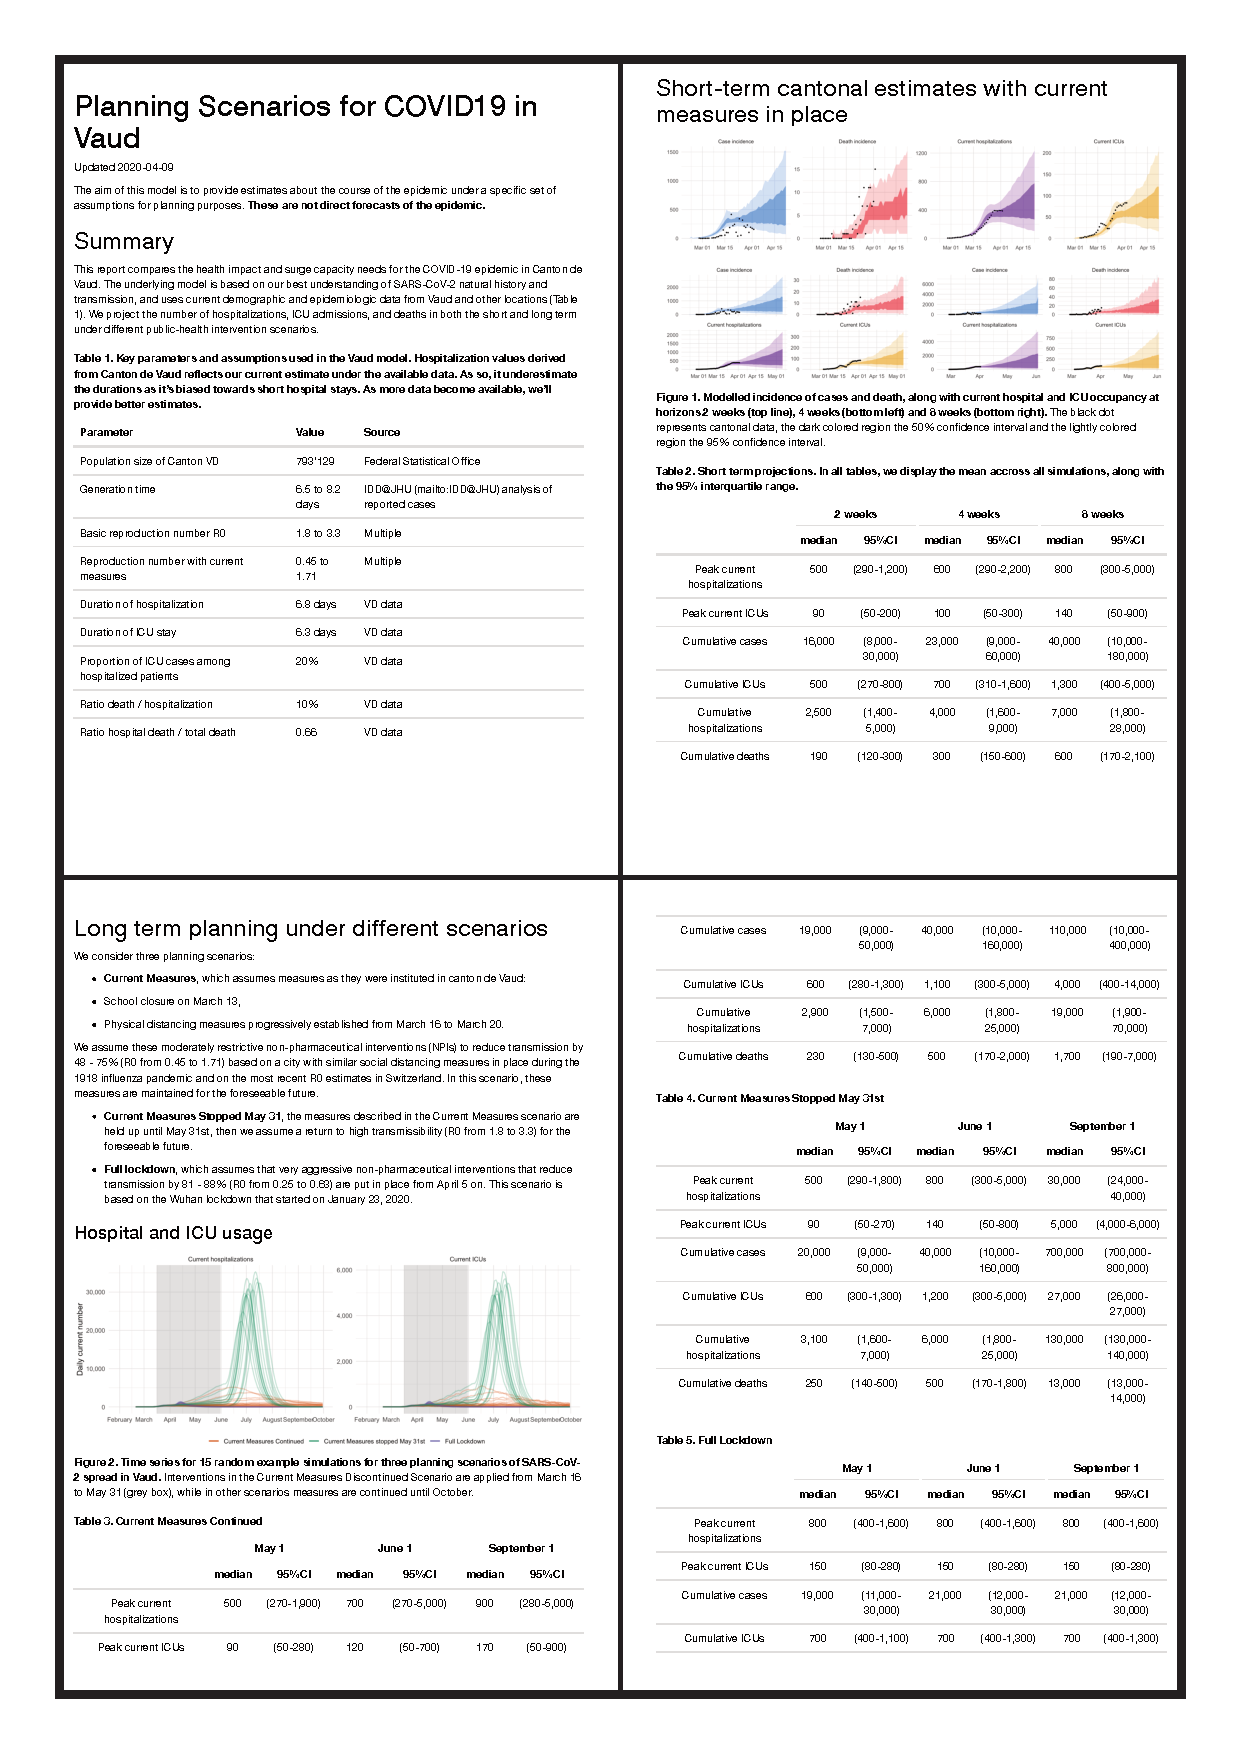
\includepdf[pages=-, pagecommand={\thispagestyle{empty}}]{fig_pipeline/planning_mod.pdf}

\section{Model Parameters from truncated data}
While collaborating with CHUV on these reports, access to precise hospitalization data was granted. It allowed us to refine our estimates\cite{Rees:COVID19LengthHospital:2020} of stays in hospital and the load of the earlth system. This section is published in the supplementary material of
\fullcite{Lemaitre:AssessingImpactNonpharmaceutical:2020}.
\begin{figure}[!htb]% [width = .7\textwidth]
    \centering
        \caption[Age distribution of patients hospitalized for COVID-19 in the canton of Vaud]{Age distribution of patients hospitalized for COVID-19 in the canton of Vaud up to April 14. Hospitalized individuals are divided in two subgroups depending on if they were treated in ICU (left) or not (right) during their stay. Moreover, only the 777 patients with known outcome are displayed here. The outcome is highlighted:  either death (orange) or discharge/transfer to another hospital (blue).}
    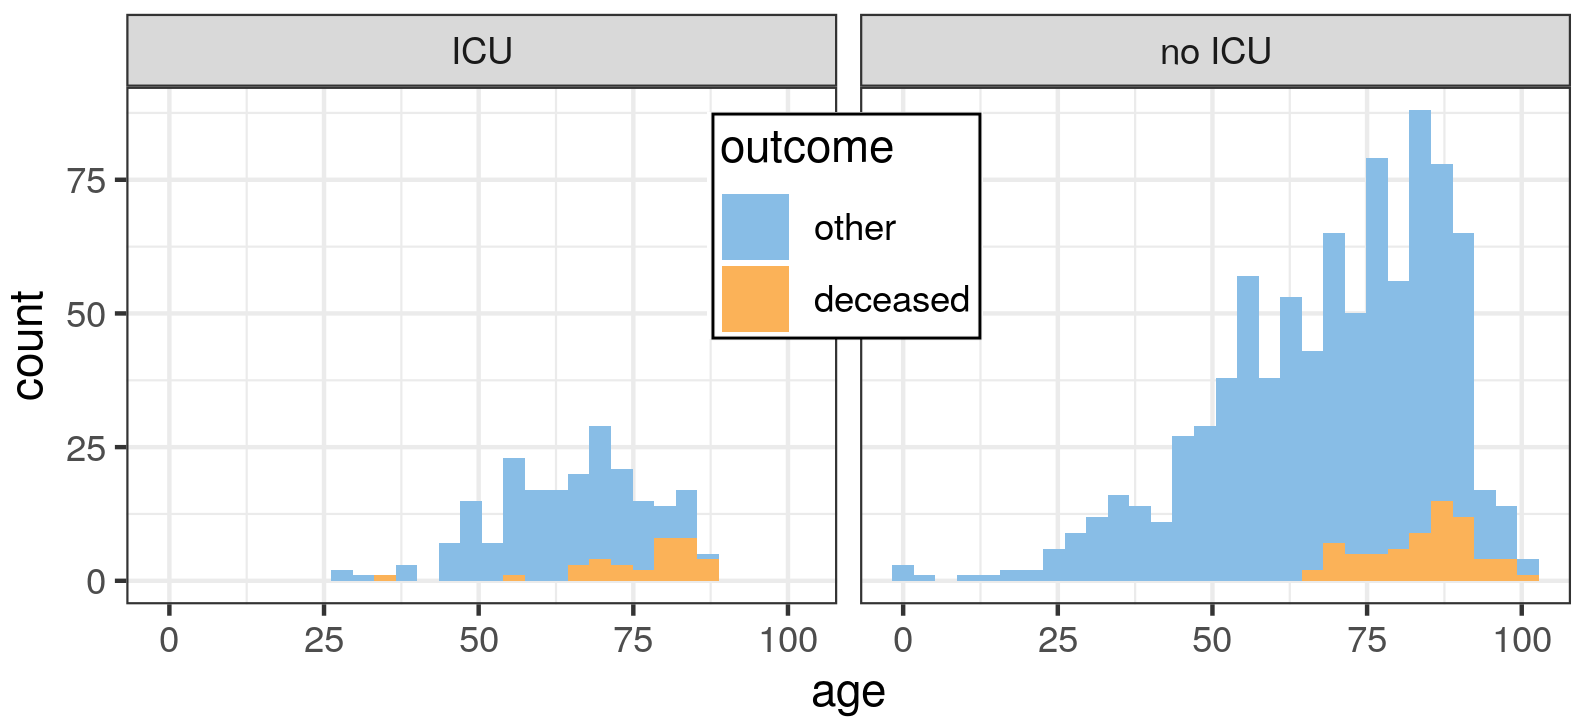
\includegraphics{fig_covid-switzerland-npi/fig_supp/VD_hist_age_mod.png}
    \label{fig:vdage}
\end{figure}
\begin{figure}[!htb]
    \centering
    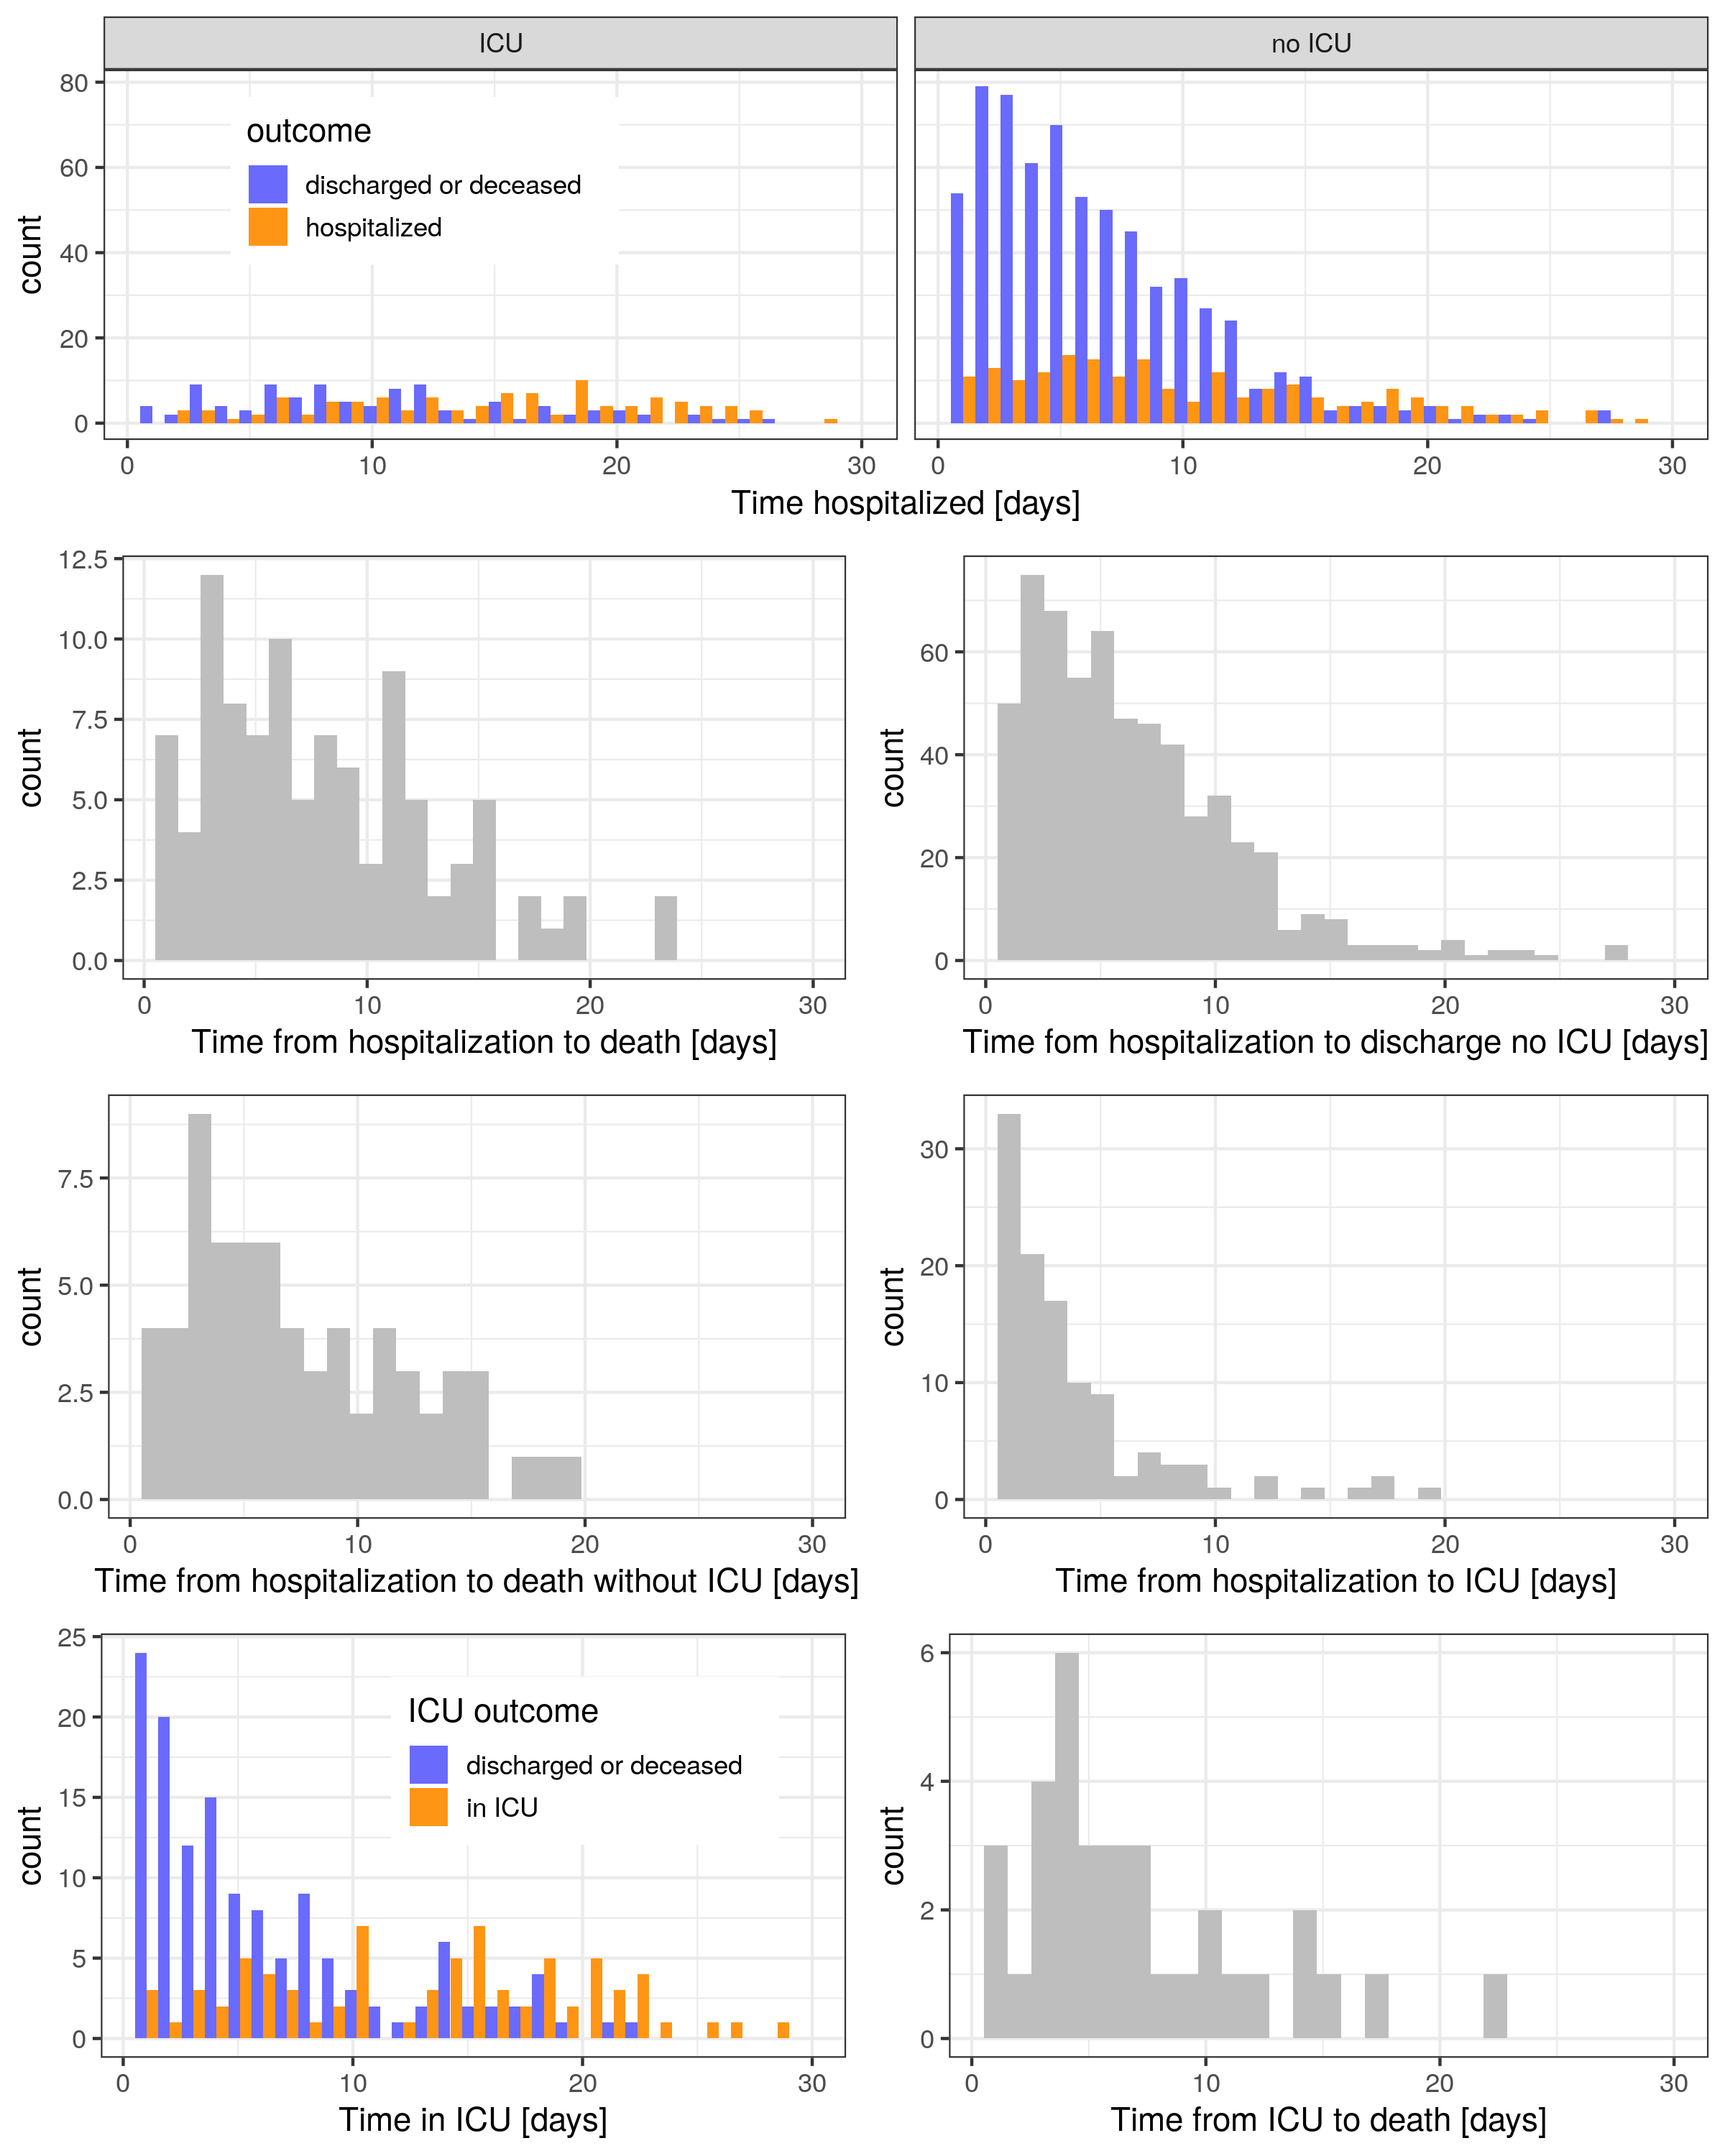
\includegraphics{fig_covid-switzerland-npi/fig_supp/VD_times.png}
    \caption[Key data of hospitalization events in canton de Vaud]{Data from canton de Vaud showing times to key hospitalization events. In order to perform this analysis, the patients are splitted in two categories: those who did not go through ICU during their stay and those who did. From left to right, top to bottom: total length of hospital stay for patients that went to ICU, then similarly for patient that did not. Then the time to death is shown for all patients, followed by both the time to discharge and to death for non-ICU patients. The last three graphs concerns ICU patients and detail ICU focused estimate: time from hospitalization to ICU, time in ICU and time from ICU to death. When meaningful, both currently hospitalized patient (orange) and already out-of-hospital patients (blue) are shown.}
    \label{fig:vdtimes}
\end{figure}


Access to individual-level data from 1093 patients, hospitalized in the canton of Vaud up to April 14, 2020 was granted. Of all patients, 41\% (448/1093) were female and 59\% were male (645/1093) with a median age of 70 years (Supplementary Material, SM, Figure~\ref{fig:vdage}). Of all the hospitalized cases, 20\% (214/1093) required use of an Intensive Care Unit (ICU).


Of 777 patients with a known outcome on April 14, 104 died (13\%). 
The hospitalized Case Fatality Ratio (hCFR) is estimated by adjusting for the distribution of time hospitalization to death accounting for the fact that outcomes have not been yet observed for all patients (right-censoring). To account for multiple outcomes (death and discharge), a parametric competing risk survival model similar to that of\cite{Ghani:MethodsEstimatingCase:2005} is implemented. A Bayesian approach proposed in\cite{Bellot:TreebasedBayesianMixture:2018} is choosen, that enables us to fit parametric distributions to times to events using accelerated failure models. This method allows for the joint estimation of the probability of each event type and the distributions of times to events. In this case the probability of death, i.e. the hCFR. A COVID-19 modeling study in France identified mixtures of probabilities of times to death, with a group dying faster with exponentially-distributed times and one dying slower\cite{Salje:EstimatingBurdenSARSCoV2:2020}. The Bayesian survival framework is extended to test for mixture in times to death and recovery. Model patients being discharged from ICU and subsequently dying, which was the case for 4/138 patients with known outcome, are not taken into account. Neither are accounted for multiple ICU stays per patient since this information was not availabe. Both Gamma and Log-Normal distributions are fitted separately to patients that did not go into ICU, and patients that did. For the former, it is modeled times from hospitalization to death or discharge, and for the latter times from ICU entry to both outcomes. Models were fit with Stan\cite{Carpenter:StanProbabilisticProgramming:2017}, and selection was done using Bayesian leave-one-out cross-validation\cite{Vehtari:PracticalBayesianModel:2017}. \\
\begin{figure}[!htb]
    \centering
        \caption[Survival functions of death and discharge for hospitalized patients and patients in ICU][-3\baselineskip]{Survival functions of death and discharge for hospitalized patients and patients in ICU. The lines represent the mean estimated cumulative probability of dying (full) and 1 minus the cumulative probability of discharge (dotted) estimated with non-parametric (Aalen-Johansen estimator, shading gives the 95\% CI) and parametric (assuming gamma and log-normal distributions, shading indicate the 95\% CrI) methods. Time is in days from hospitalization for patients that did not require ICU, and time from ICU admission for those that did. The point at which the lines join represents the probability that the final outcome is death, which was estimated to be 28.1\% (95\% CrI: 16.4-40.9) for patients in ICU and 13.0\% (95\% CrI: 9.9-16.6) for patients not requiring ICU based on the log-normal distribution.}
    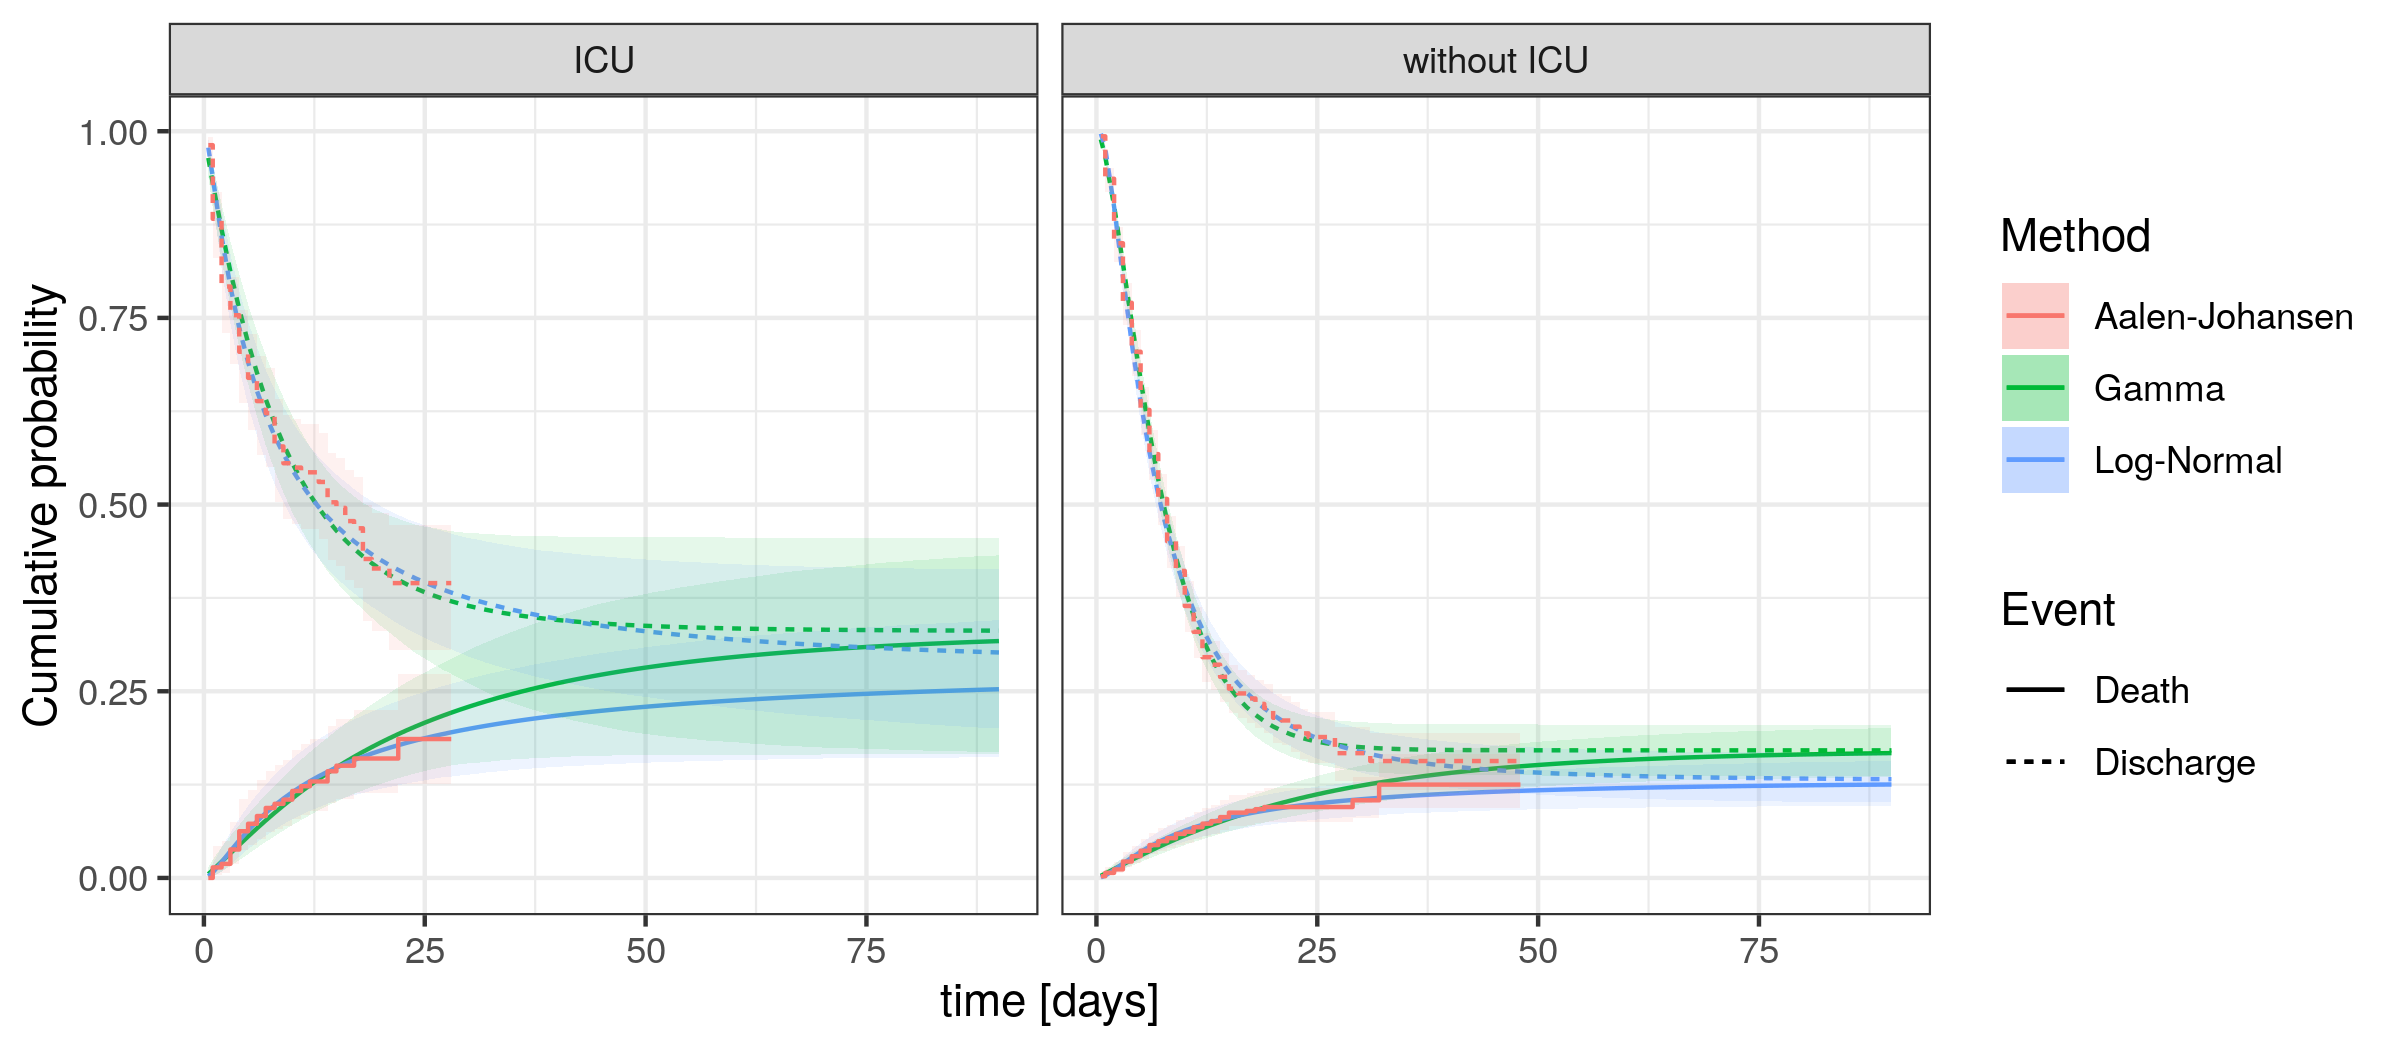
\includegraphics{fig_covid-switzerland-npi/fig_supp/survival_analaysis.png}
    \label{fig:delays}
\end{figure}


Times to death and discharge were best described by log-normal distributions with a single group both for patients having required ICU or not (Fig.~\ref{fig:delays}). When accounting for right-censoring and assuming log-normally distributed times to events, an overall hCFR is estimated at 16.0\% (95\% credible interval, CrI: 12.5-19.8), resulting from a hCFR of 28.1\% (95\% CrI: 16.4-40.9) for patients requiring ICU and 13.0\% (95\% CrI: 9.9-16.6) for patients that did no require it. Estimated hCFRs were slightly higher when assuming gamma-distributed times to events (overall hCFR of 20.3\%, 95\% CrI: 15.9-24.1).


\noindent The distribution of times of hospitalization processes are shown in Fig.~\ref{fig:vdtimes}, and fitted distribution parameters given in Table~\ref{tab:vdparams}.


\begin{table}[t]
\caption[Observed hospitalization time distributions.]{Observed hospitalization time distributions. All times are in days and taken from the date of hospitalization if not specified otherwise. Note that these estimates are biased due to right-censoring of observations and probably under-estimate the true distributions.  Table~\ref{tab:survpars} shows estimates that account for right-censoring.}
\label{tab:vdparams}
\centering
\begin{tabular}{lrrrr}
\toprule
 & mean & sd & mean (logscale) & sd (logscale)\\
\midrule
Time hospitalized & 8.49 & 6.58 & 1.81 & 0.87\\
Time to death & 8.23 & 6.09 & 1.80 & 0.87\\ \addlinespace
Time to discharge without ICU & 6.29 & 4.66 & 1.56 & 0.80\\
Time hospitalized without ICU & 7.35 & 5.79 & 1.68 & 0.85\\
Time to death without ICU & 7.84 & 6.27 & 1.73 & 0.88\\ \addlinespace
Time to ICU & 2.35 & 3.79 & 0.18 & 1.05\\
Time hospitalized with ICU & 13.14 & 7.50 & 2.37 & 0.72\\
Time in ICU & 8.36 & 6.76 & 1.69 & 1.04\\
Time from ICU to discharge & 8.68 & 6.99 & 1.71 & 1.07\\
Time from ICU to death & 6.97 & 4.98 & 1.68 & 0.77\\
\bottomrule
\end{tabular}
\end{table}


\begin{fwtable}
    \centering
    \begin{tabular}{ccccccc}
\toprule
 & & \multicolumn{3}{c}{Log-Normal} & \multicolumn{2}{c}{Gamma}\\ \cmidrule(rl){3-5} \cmidrule(rl){6-7}
Group & Event & median & mean-log & SD-log & scale & shape\\
\midrule
Without ICU & Death & 10 (7.3--16) & 2.3 (2--2.8) & 1.2 (0.95--1.5) & 21 (21--22) & 1.1 (0.83--1.4)\\
 & Discharge & 6.1 (5.6-6.6) & 1.8 (1.7--1.9) & 0.93 (0.87--0.99) & 4.3 (4.4--4.2) & 1.8 (1.6-2)\\ \addlinespace
ICU & Death & 13 (6.2--30) & 2.6 (1.8--3.4) & 1.3 (0.87--1.9) & 21 (12--23) & 1.2 (0.74--1.9)\\
 & Discharge & 6.4 (4.3--9.3) & 1.8 (1.5--2.2) & 1.3 (1.1--1.6) & 9.1 (8.1--11) & 1 (0.75--1.4)\\
\bottomrule
\end{tabular}
\caption[Estimated parameters of hospitalization time distributions.]{Estimated parameters of hospitalization time distributions. These estimates differ from observed values given in Table~\ref{tab:vdparams} by accounting for right-censoring of observations. Time from hospitalization to discharge or death, and from ICU admission to discharge or death are reported here. Estimates were obtained using competing risk survival model as described above. Parameters are given in terms of their posterior mean and 95\% CrI (in parenthesis). For the log-normal distribution the parameters correspond to the mean and SD of the logarithm of the distribution.}
     \label{tab:survpars}
\end{fwtable}

 % 4
\begin{fullwidth}
\chapter[Assessing the impact of non-pharmaceutical interventions on SARS-CoV-2 transmission in Switzerland]{Assessing the impact of non-pharmaceutical\\ interventions on SARS-CoV-2 transmission\\ in Switzerland}
\chaptermark{Assessing the impact of non-pharmaceutical interventions on covid-19 transmission}
\label{ch:covid-switzerland-npi}

Following the rapid dissemination of \textsc{covid}-19 in Switzerland, large-scale non-pharmaceutical interventions (NPIs) were implemented by the cantons and the federal government between February 28 and March 20, 2020. Estimates of the impact of these interventions on SARS-CoV-2 transmission are critical for decision making in the present and future outbreaks. The aim of this chapter is to assess the impact of these NPIs on disease transmission by estimating changes in the basic reproduction number $R_0$ at national and cantonal levels in relation to the timing of these NPIs. For the whole country and eleven cantons, the time-varying $R_0$ is estimated by fitting a stochastic transmission model explicitly simulating within-hospital dynamics. The dataset includes individual-level data from more than 1000 hospitalised patients in Switzerland and public daily reports of hospitalisations and deaths. The national $R_0$ is estimated to be 2.8 (95\% confidence interval 2.1–3.8) at the beginning of the epidemic. Starting from around March 7, a strong reduction of the time-varying $R_0$ is found, with a 86\% median decrease (95\% quantile range [QR] 79–90\%) to a value of 0.40 (95\% QR 0.3–0.58) in the period of March 29 to April 5. At the cantonal level, $R_0$ decreased by between 53\% and 92\% over the course of the epidemic. Reductions in time-varying $R_0$ were synchronous with changes in mobility patterns as estimated through smartphone activity, which started before the official implementation of NPIs. Most of the reduction of transmission is inferred to be attributable to behavioural changes as opposed to natural immunity, the latter accounting for only about 4\% of the total reduction in effective transmission. As Switzerland considers relaxing some of the restrictions of social mixing, current estimates of time-varying $R_0$ well below one are promising. However, as of April 24, 2020, at least 96\% (95\% QR 95.7–96.4\%) of the Swiss population remains susceptible to SARS-CoV-2. These results warrant a cautious relaxation of social distance practices and close monitoring of changes in both the basic and effective reproduction numbers.

This chapter is based on:
\longfullcite{Lemaitre:AssessingImpactNonpharmaceutical:2020}, and J. Perez-Saez shares co-authorship of the work. It  is referred in the following as the postprint (and its supplementary information \textsc{si})
\end{fullwidth}

\section{Introduction}
As of May 13, 2020, the ongoing coronavirus disease 2019 (\textsc{covid}-19) pandemic caused by severe acute respiratory syndrome coronavirus 2 (SARS-CoV-2) has resulted in more than 4.1 million cases and 280,000 deaths globally\cite{WHO:WHOSituationReport:2020}. Independent estimates of the basic reproduction number $R_0$ for SARS-CoV-2 from the initial phases of the epidemic in China, Europe and the United States have generally ranged from 2–3\cite{Riou:PatternEarlyHumantohuman:2020} with doubling times on the order of 2–4 days. In response to the rapid increase in reported cases and hospitalisations, most countries have implemented non-pharmaceutical interventions (NPIs), including compulsory face mask use, border and school closures, quarantine of suspected and confirmed cases, up to population-wide home isolation\cite{HITCOVIDTeam:HealthInterventionsTracking:2020}. An observation study conducted in Hong Kong during this pandemic estimated that social distancing measures and school closures reduced \textsc{covid}-19 transmission, as characterised by the effective reproductive number, by 44\%\cite{Cowling:ImpactAssessmentNonpharmaceutical:2020}. Comparable reductions have been observed in many different settings\cite{Flaxman:Report13Estimating:2020}. Making decisions around relaxing NPIs requires both a careful assessment of the level of pre-relaxation transmission (e.g., $R_0$) and quantification of the expected increase in transmission from relaxation of different NPIs. 

From the initial reported case on February 24 to April 29, Switzerland reported more than 24'400 laboratory confirmed COVID-19 cases and 1'408 official deaths affecting all 26 cantons\cite{OFSP:RapportSituationEpidemiologique:2020}. The federal government issued a series of special decrees from February 28 banning gatherings of more than 1'000 people culminating on March 20 recommended home isolation (fig.~\ref{fig:covid-ch-data}). One month after the first NPI, daily confirmed case incidence had decreased from a peak of more than 1000 to a daily average of under 170 in the week of April 20–26 (fig.~\ref{fig:covid-ch-data}). Initial reports have suggested a basic reproduction number ($R_0$) of 3.5 at the start of the epidemic, with a decrease of 85\% by March 20\cite[-3\baselineskip]{Flaxman:Report13Estimating:2020}.
\begin{figure*}\centering
  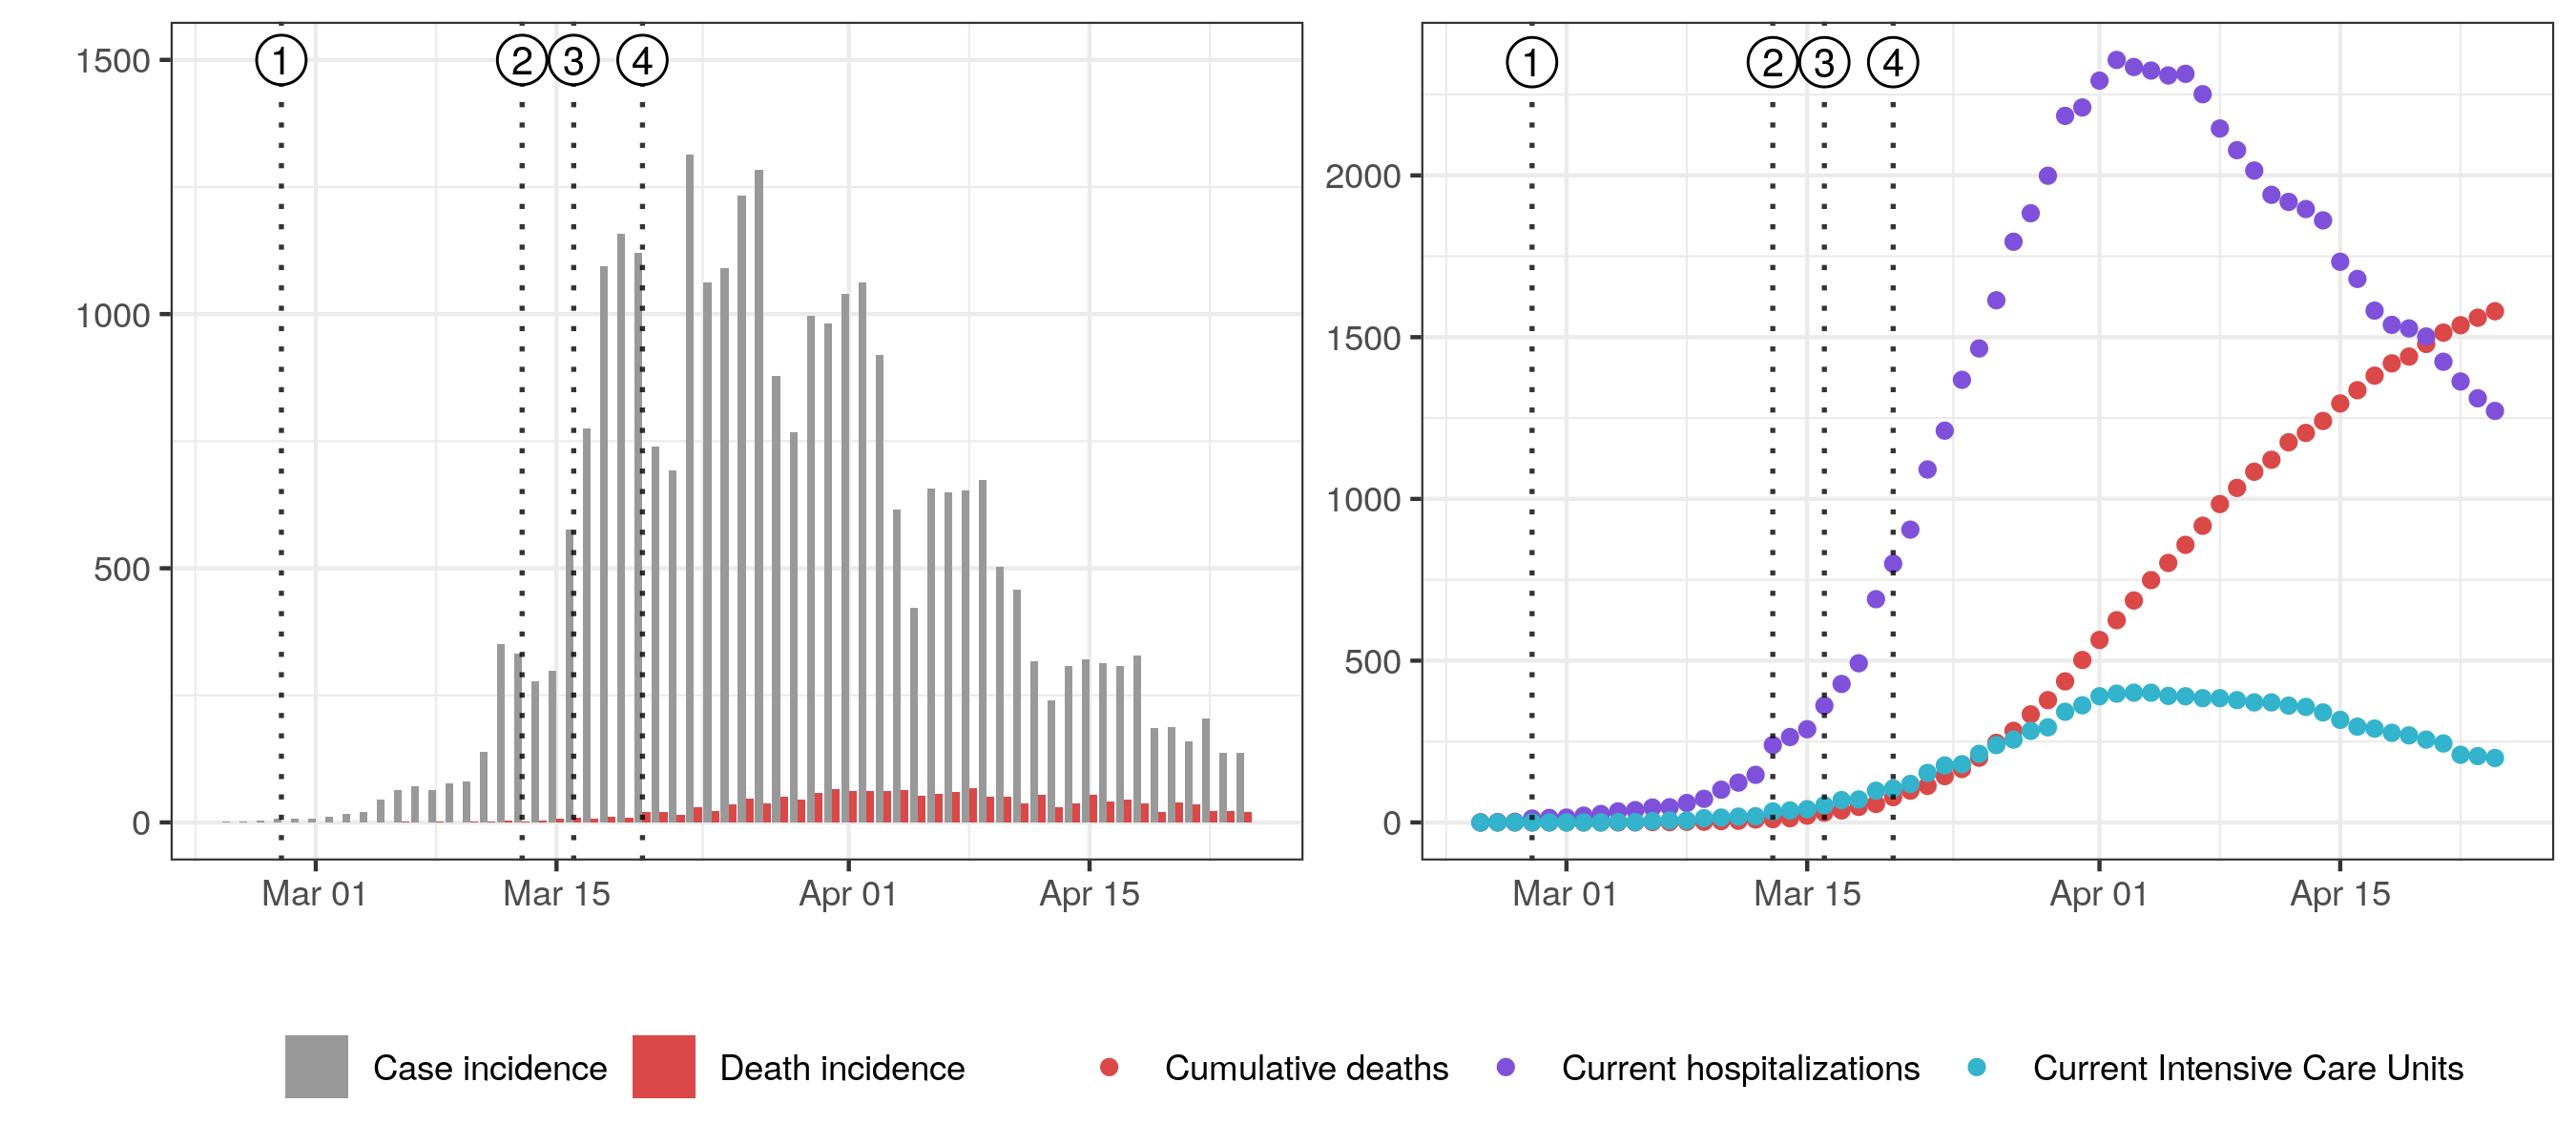
\includegraphics[width=\textwidth]{fig_covid-switzerland-npi/FIGURE_1.png}
  \caption[\textsc{covid}-19 epidemic curve in Switzerland and timing of interventions]{\textsc{covid}-19 epidemic curve in Switzerland and timing of non-pharmaceutical interventions. Dotted lines indicate the issuing of NPIs: (1) ban on gatherings of more than 1'000 people, (2) school closure, (3) closure of non-essential activities, and (4) ban on gatherings of more than five people. Left: Daily case incidence at time of reporting along with death incidence. Right: Current hospitalisations, intensive care units (ICUs) and cumulative deaths. Data from \textcite{Probst:DaenuprobstCovid19casesswitzerland:2020}, and may therefore present inconsistencies with official reports from the Federal Office of Public Health% due to reporting delays.
  }
  \label{fig:covid-ch-data}
\end{figure*}
 However, these estimates, part of a multicountry analysis of NPIs, relied on death incidence and did not account for specifics of the hospitalisation processes in Switzerland. Moreover, changes in $R_0$ were assumed to be on the date of NPI implementation, thus not allowing for the exploration of the relative timing between NPIs and changes in transmission. Furthermore, such delays likely bias the estimate $R_0$. 

NPIs affecting daily activities such as school closures and gathering bans aim at having a direct impact on mobility patterns to reduce potentially infectious social contacts. In other terms, the causal pathway from NPIs to transmission reduction is mediated by changes in mobility. Recent releases of mobility data from smartphone software providers give the possibility to study the associations between the implementation of movement-limiting measures, behavioural change and the related changes in $R_0$. Context-specific data on the degree and speed of compliance with these types of NPIs and associations with the observed decreases in $R_0$ could inform scenario-building should the future reinstatement of measures become necessary. Given that $R_0$ directly represents transmission potential, its quantification enables us to estimate the proportion of reduction in transmission attribuable to behavioral changes. In this sense, tracking of $R_0$ is more suited to study the impact of NPIs than the effective reproduction number $R_{eff}$, which is an aggregate measure of transmission capturing aspects of both infectious contacts and of population susceptibility. 

Here, the goal is to estimate the changes in $R_0$ over the course of the epidemic at both the national and cantonal levels using detailed data on hospitalisations and deaths from Switzerland between February 24 and April 24. In order to understand the estimated changes in $R_0$, its relationship with the timing of NPIs and human mobility estimates derived from cell phone data is explored.

\section{Methods}
The setting for the present chapter arose while providing scenario modeling reports, as presented in \textsc{Chapter~4}. CHUV, the hospital coordinating Canton de Vaud response, provided access to individual hospitalization data. The dataset and processing to account for right-censoring are presented in the \textsc{Appendix to Chapter~5}. This dataset allowed for refined estimates of stays in hospital and death processes, which in turn were used as assumptions in a \textsc{covid}-19 model; giving said model sufficient stiffness to estimate $R_0$ in time. Model equations and fixed and inferred parameter values are left in the postprint \textsc{si}.

\subsection{Model and assumptions}
\paragraph{Model Structure} A stochastic compartmental model of the \textsc{covid}-19 epidemic and hospitalisation processes is developed for each canton of Switzerland. The model is structured around the classical S, E, I and R compartments\cite{Kermack:ContributionMathematicalTheory:1927}, and the model diagram is shown in fig.~\ref{fig:covid-ch-diagram}. %Namely, the population is divided in compartments depending on their status with regard to \textsc{covid}-19. 
A susceptible individual $S$ might be exposed after contact with infectious $I$ individuals. Upon exposure, a formerly susceptible individual goes through an incubation period $E$ before becoming infectious $I$. The individual then recovers $R$ and does not participate in transmission anymore. 
%In addition to these dynamics, some proportion of infectected invididuals develop severe disease and among those, some are hospitalised and may advance to needing the intensive care unit. 
In addition to these dynamics, infected individuals have some probability of developing severe symptoms. Estimates derived from data from the canton of Vaud, as shown in the  show a high proportion of deaths outside of hospitals ($\approx 50\%$) hence two pathways are modeled depending if the individual seek  or has access to hospital care.  Some severly infected will be treated in a hospitals after a delay from symptom onset $I_h$. In this case, hospitalization lead to discharge (recovery) or death, either through normal hospitalization ($H_{s}$ and $H_d$ respectively) or passing through Intensive Care Units (ICUs, compartments $U_{s}$ and $U_d$ respectively). Otherwise, severly infected may recover or die without passing through hospitalization, going into compartment $I_d$. There is no need to explicitly model a latent stage where individuals are still asymptomatic but infectious\cite[-8\baselineskip]{Ganyani:EstimatingGenerationInterval:2020,He:TemporalDynamicsViral:2020, Liu:ContributionPresymptomaticInfection:2020} as only hospitalisation and death data is used. The model is implemented as a hidden markov model using the pomp R package\cite[-3\baselineskip]{King:StatisticalInferencePartially:2015}. 
 \begin{figure}[!htb]
\begin{center}
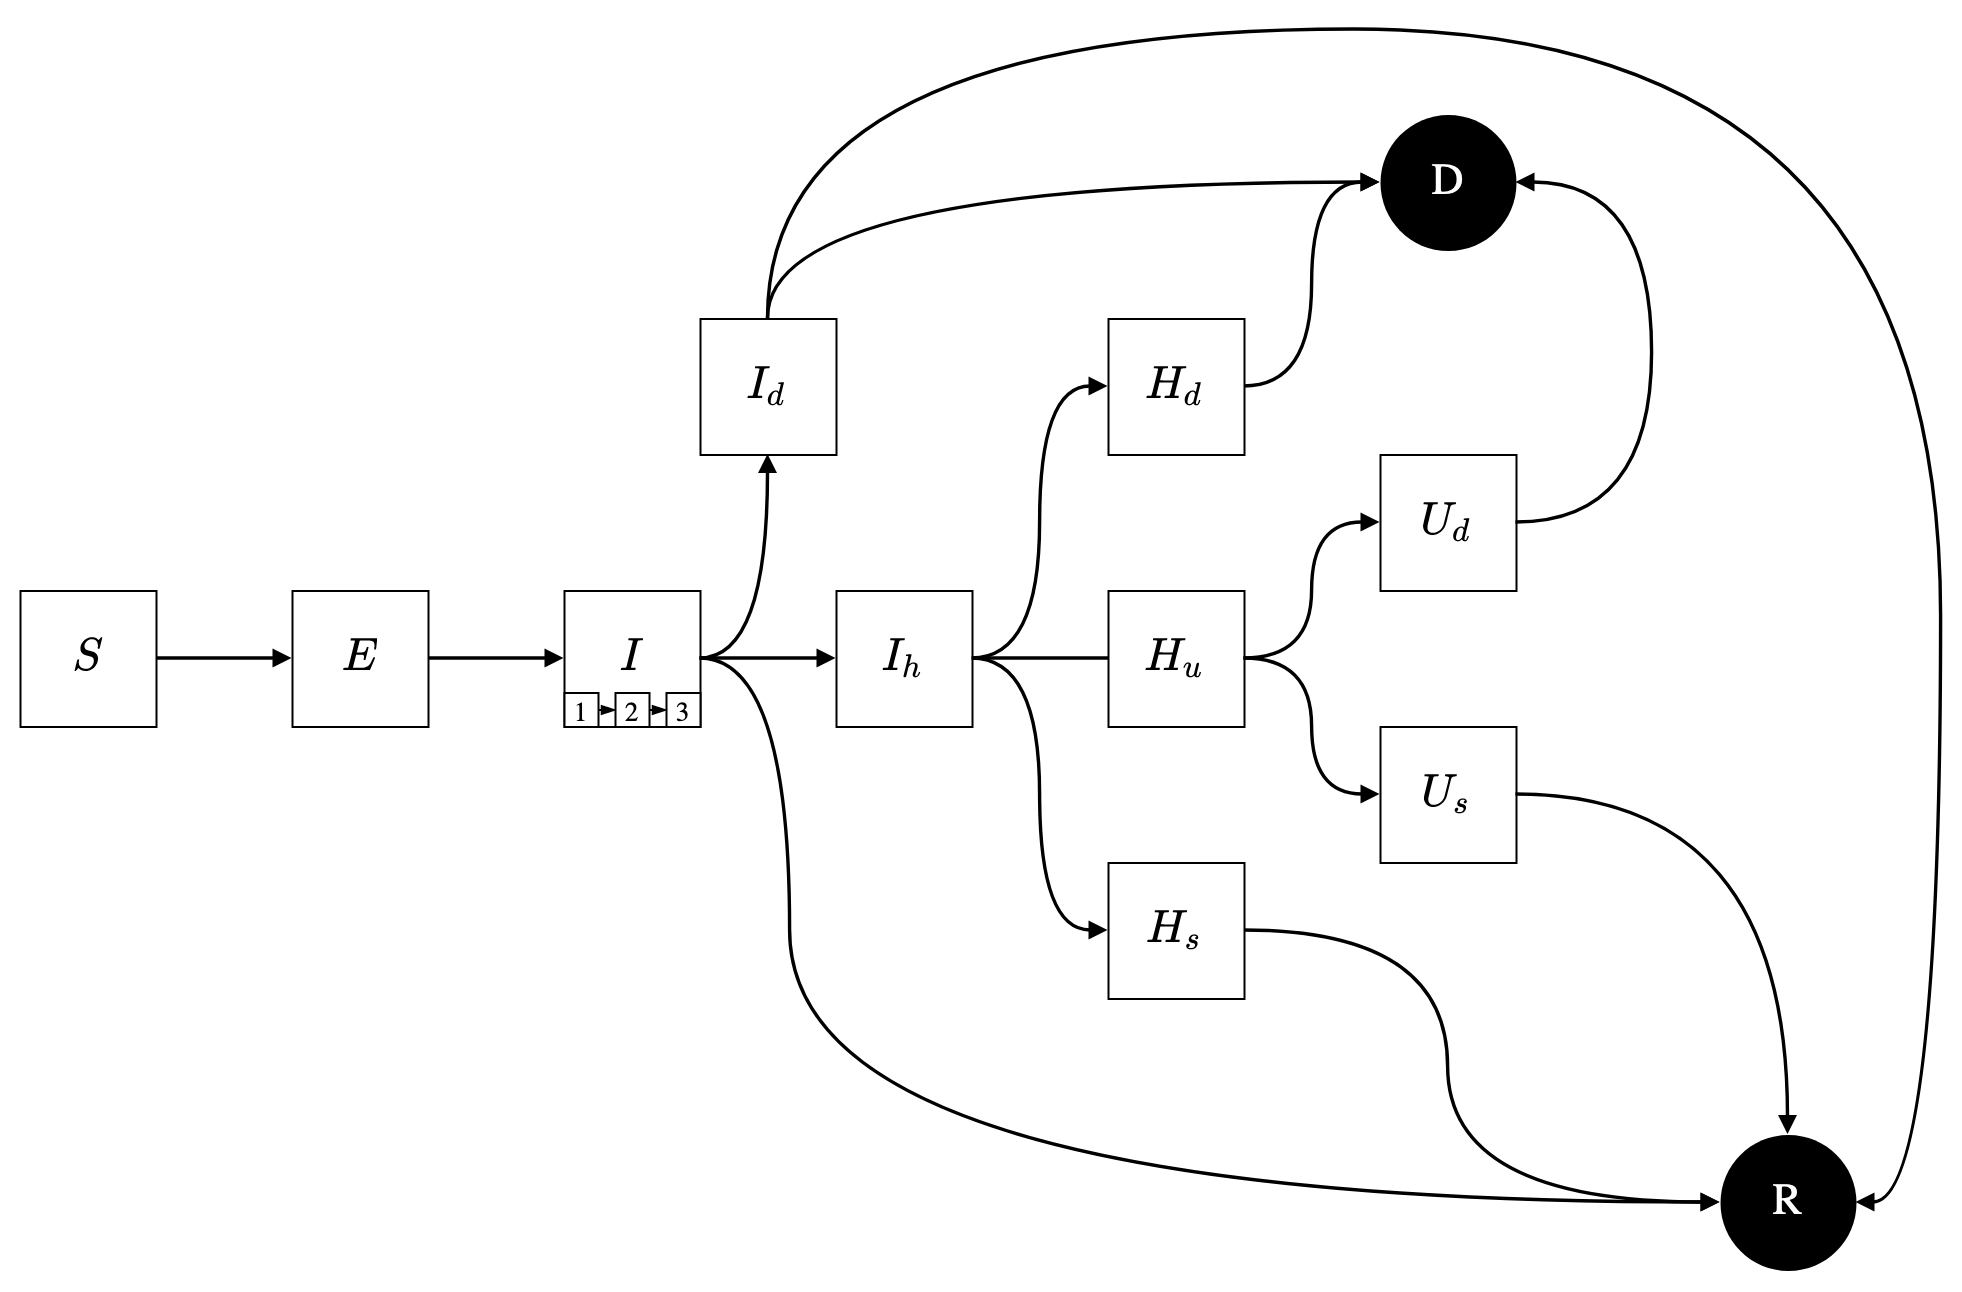
\includegraphics{fig_covid-switzerland-npi/fig_supp/diagram.png}
\caption[Schematic diagram of \textsc{covid}-19 transmission and hospitalization processes]{Schematic diagram of \textsc{covid}-19 transmission and hospitalization processes. There are two sinks: Death $D$ and recovered $R$. Each stage with regard to the disease may be implemented with several compartments (subscript numbered boxes) to better represent the time distribution spent in that stage.}
\label{fig:covid-ch-diagram}
\end{center}
\end{figure}

\paragraph{Assumptions} The reader is referred to the postprint \textsc{si} for the exhaustive description of model transitions and parameters. As parameter indentifiability is needed to capture the dynamics of $R_0$, most of the parameters were fixed to values from the litterature or obtained analyzing the data from Canton de Vaud\footnote[][-3\baselineskip]{As noted by Gostic et al., the accuracy of $R_0$ estimates obtained with the method presented here is sensible to assumptions on model structure and parameters; see \fullcite{Gostic:PracticalConsiderationsMeasuring:2020a}.}.
The transmission model is parameterized assuming a mean generation time of 5.2 days\cite{Ganyani:EstimatingGenerationInterval:2020}, and an exposed and non-infectious duration of 2.9 days\cite{He:TemporalDynamicsViral:2020}, yielding a mean duration of 4.6 days in the infectious compartments.  It is assumed that 7.5\% of infections were severe and would require hospitalisation, that 50\% of deaths happened outside of hospitals (from data on Canton de Vaud described in the \textsc{Appendix}, and data from Geneva collected from OpenZH), that 16\% of those hospitalised would die (data from Vaud, see \textsc{Appendix}), and that the infection fatality ratio (IFR) was 0.75\%, which is in the range of published estimates\cite{Verity:EstimatesSeverityCoronavirus:2020, Russell:EstimatingInfectionCase:2020}. Individual-level data on hospitalised cases from the canton of Vaud is used to estimate the distribution of time spent in the hospital and in the intensive care unit (ICU). Times to discharge and death are estimated using survival models that account for right-censoring of observations (see \textsc{Appendix}). The number of compartments for the linear-chain trick (\ie the shape parameter for the erlang distributed residence time) for each observable hospitalization state was obtained by fitting Erlang distributions to the data of canton de Vaud. To account for right-censoring the model is fitted to the estimated log-normal distributions described in the \textsc{Appendix} instead directly to observed times to events but rather. The rate parameter of the Erlang distributions is calibrated for shape parameters between $1$ and $10$ by minimizing the Kullback-Leibler (KL) divergence between the Erlang and estimated log-normal distributions. The final fit was taken to be the one with the smallest KL-divergence. We found that all hospitalization processes were best represented with exponential distributions (Erlang with shape parameter of $1$)\footnote{In the first preprinted version without the survival analysis, the shape parameters were estimated to be around 2, which highlights the importance of carefully processing data and reasoning about potential biases before using it.}.

\subsection{Data and Inference} 
\paragraph{Dataset} Curated data from OpenZH\cite[3\baselineskip]{openZH:OpenZHCovid19:2020} up to April 24 is used. This dataset included, by canton, the number of hospitalised \textsc{covid} patients, and the cumulative numbers of deaths, cases and hospital discharges; the latter not available for all cantons. The cantonal estimate is focused on cantons that had enough cases and data to obtain meaningful results, keeping 11 of the 26 cantons (Bern, Basel-Landschaft, Basel-Stadt, Fribourg, Geneva, Jura, Neuchâtel, Ticino, Vaud, Valais and Zurich). These cantons account for 66\% of the Swiss population. The national estimate uses curated national aggregate data and thus encompassed all cantons\cite{Probst:DaenuprobstCovid19casesswitzerland:2020}. Unknown parameters the model are fitted using maximum likelihood inference through iterated filtering\cite{Ionides:InferenceDynamicLatent:2015}. No attempt to include confirmed case data into the observation model were made because of the heterogeneous testing strategies adopted across cantons and over time. The model is therefore fitted to death incidence and changes in current hospitalisations using appropriate likelihood functions:
\begin{equation}
\begin{split}
 \text{deaths}(t) &\sim \text{Poisson}(\Delta D(t)) \\
\Delta  \text{hosp}(t) &\sim \text{Skellam}(\Delta H(t), \Delta D_H(t) + \Delta R_H(t)) \\
\end{split}
\end{equation}
\noindent where, $\Delta D(t)$, $\Delta H(t)$, $\Delta D_H(t)$, $\Delta R_H(t)$ are respectively the number of new deaths, hospitalized, and deaths and discharged from hospitals at time $t$, and $\Delta \text{hosp}(t)$ is the difference between the number of current hospitalizations at times $t$ and $t-1$, for which a Skellam distribution\footnote{which represents the difference between two independent random variables, each Poisson-distributed. See \fullcite{Skellam:FrequencyDistributionDifference:1946}.} is choosen. The full log-likelihood of the observation model was taken as the sum of the individual log-likelihoods of the $\Delta \text{hosp}(t)$ and of the $\text{deaths}(t)$. 
The model is calibrated separately for each canton on the daily death and hospitalization until April 24. Hospitalisation incidence data at the cantonal level would have provided more information, but this data was not accessible. Fitting to hospitalisation incidence data, which access was granted in the canton of Vaud, yielded similar results to those when changes in current hospitalisations were used. The majority of model parameters was either derived from Vaud data or from the litterature (see postprint \textsc{si}), it enables the identifiability of the reproduction number $R_0$.
 
 \paragraph{Reproduction number estimation} Time-varying basic reproduction numbers $R_0$ were estimated following a similar approach to Cazelles et al.\cite{Cazelles:AccountingNonstationarityEpidemiology:2018}, recently applied to \textsc{covid}-19 transmission in Hubei\cite{Kucharski:EarlyDynamicsTransmission:2020}. The method aims at inferring the time series of $R_0$\footnote{As mentionned, $R_0$, not $R_{eff}$ is computed as the presented method estimates the basic reproduction number, \ie the expected number of infections generate by one infected individual in a fully susceptible population. To do so, the susceptible and recovered population explicity modeled while other methods usually compute the effective reproduction number in the population by deconvolution on observed data.} that yields model dynamics that are in best agreement with the whole set of available observations. As such, the value of $R_0$ at a given point in time is informed by the whole data, and therefore does not have the limitations of being either “forward looking” or “backwards looking” as it is the case of commonly used statistical methods applied for this purpose\cite{Wallinga:DifferentEpidemicCurves:2004,Cori:NewFrameworkSoftware:2013,Lipsitch:CommentPanLiu:2020}. 
 
The model equations are similar to the previously presented partially-observed Markov Processes models, and are left in the postprint \textsc{si}. The difference lies in the force of infection. Given the state of the system at time \(t\), \(\mathcal{X}_t\), and using the same notations as in \textsc{Chapter~3}, the transition $S \longrightarrow E$ model reads:

\begin{gather}
\begin{aligned}
    \mathbb{P}\left[ \Delta N_{SE}(t) = 1 \mid\mathcal{X}_t\right] &=  \underbrace{\beta(t)  \frac{I_1(t) + I_2(t) + I_3(t)}{P}}_{\text{Force of infection} S(t)} \Delta t + o(\Delta t)\\
    \end{aligned}
\end{gather}

Time-varying $R_0(t) = \beta(t)/(3r_I)$ is modelled as a geometric random walk defined by its calibrated variance, where $\beta$ is the transmission parameter and $1/(3r_I)$ is the mean duration spent in the infectious compartments $I_1$ to $I_3$. Once the time series was inferred, the timing and slope of changes in $R_0$ is evaluated by using linear changepoint models\cite{Lindelov:McpPackageRegression:2020}. The null model corresponded to a linear decrease between two plateaus corresponding to the baseline value at the start of the epidemic and a low value after the implementation of NPIs. To allow for different slopes in the decreasing phase of $R_0$, models with one and two additional breakpoints (corresponding to two and three different slopes) are also fitted, and the best model was selected using Bayesian model selection based on leave-one-out cross-validation (details in section 6 of the postprint \textsc{si}). 

The estimated changes in $R_0$  were constrasted with changes in activity-related mobility data produced by Google\cite{GoogleLLC:GoogleCOVID19Community:2020}. Changes in activity were expressed as relative changes with respect to a baseline computed as the median over a 5-week period from January 3 to February 6. Mobility changes were computed for different categories: grocery and pharmacy, parks, transit stations, retail and recreation, residential, and workplace. Mobility estimates were based on smartphone-based geo-location location data (GPS, WiFi connections, Bluetooth) from users who activated Location History for their Google Account. These data were used to determine changes in the number of visits to and length of stays in locations categorized into the above-mentioned types. The dataset therefore only covers a sample of the Swiss population who use smartphones, the latter representing around 80\% of the total population in 2020\cite{ODea:SmartphoneUsersSwitzerland:2020}. Gaps in the dataset were filled with linear interpolation and a 7-day moving average was applied to smooth out weekly seasonality in activities. The cross-correlation between changes in $R_0$ and the averaged changes in each type of activity was computed with lags up to 10-days. Changes in $R_0$ were computed based on location-specific baselines taken as the mean value of $R_0$ from the beginning of the simulations, 5 days before the first reported case in each canton, until March 8. Changepoint models are employed identify dates of change in mobility patterns and in $R_0$. \marginnote[-5\baselineskip]{All data and code except for individual hospitalisation data from Canton of Vaud have been deposited on Zenodo (\url{doi.org/10.5281/zenodo.3862075}). The change point analysis, model fit and additional results are omitted from this thesis and may be found in the supplementary information of \parencite{Lemaitre:AssessingImpactNonpharmaceutical:2020}}


\section{Results}
\begin{figure*}\centering
  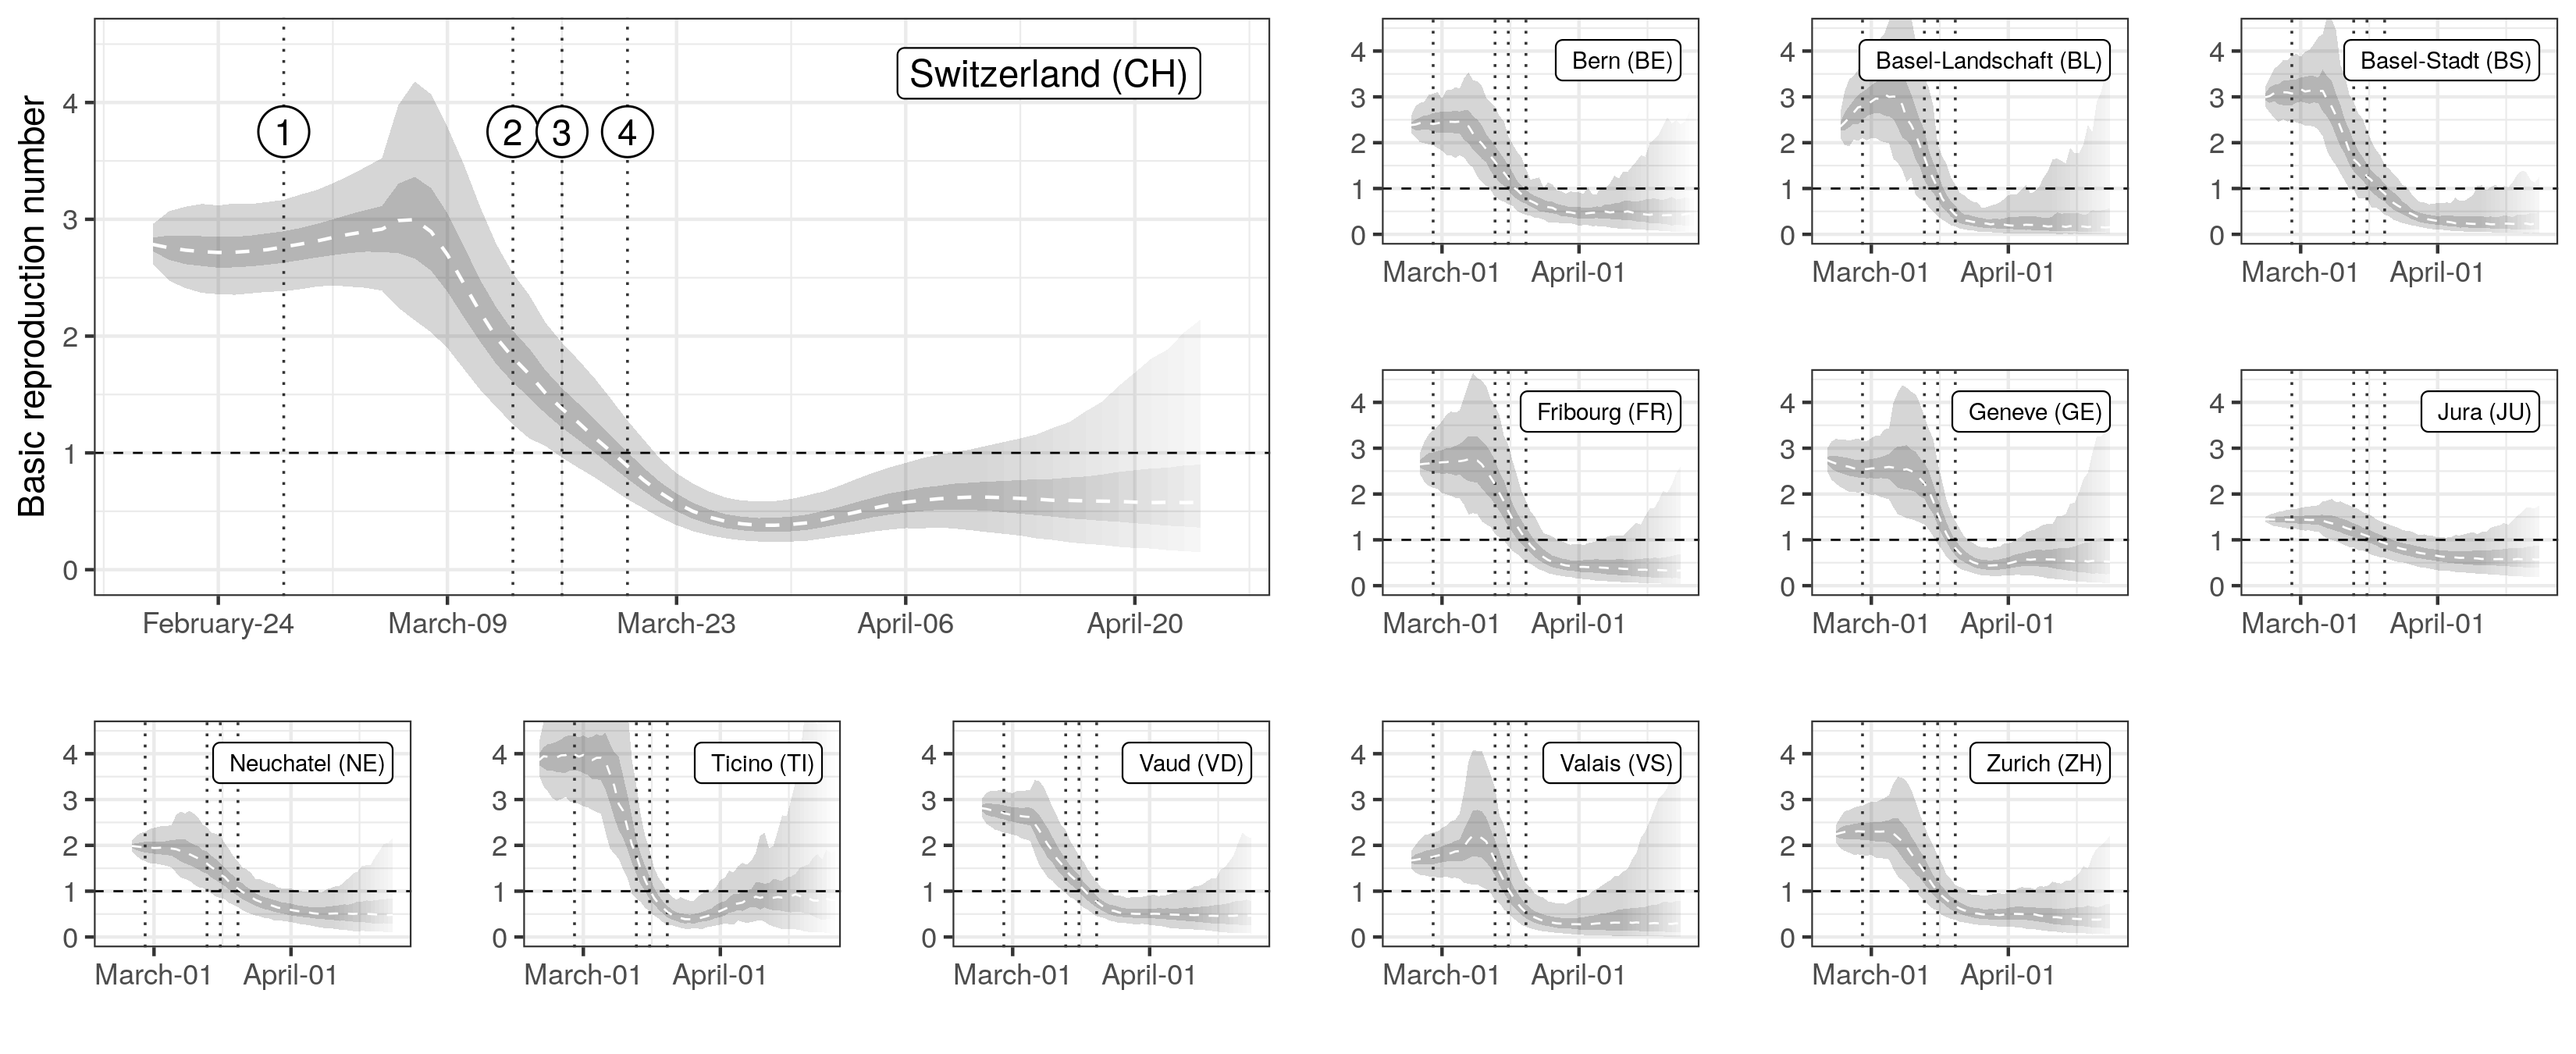
\includegraphics[width=\textwidth]{fig_covid-switzerland-npi/FIGURE_2.png}
  \caption[Estimates of changes in the basic reproduction number $R_0$][-1\baselineskip]{Estimates of changes in the basic reproduction number $R_0$. Median (dashed line), IQR (dark gray) and the 95\% QR (light gray) of the estimated time series of $R_0$ are shown for each canton. Vertical dotted lines indicate the issuing of NPIs as described in fig.~\ref{fig:covid-ch-data}. Transparency at the end of the time series indicates increasing uncertainty (style inspired by the reports of CMMID.}
  \label{fig:covid-ch-r0}
\end{figure*}
Over the study period $R_0$ trends follows a common trajectory nationally and across cantons, starting with a high plateau ($R_0 >2$) in the early stage of the epidemic followed by a rapid reduction starting at the beginning of March, and reaching a low and stable value ($R_0 <1$) from end of March onwards (fig.~\ref{fig:covid-ch-r0}). 

At the beginning of the epidemic, $R_0$ is estimated at 2.8 (95\% confidence interval [CI] 2.06–3.83) at the national level, with cantonal-level values ranging from 2.5 to 3.1 (postprint \textsc{si} tab. 5). The onset of the reduction was estimated to be between March 4 (Basel-Stadt and Vaud) and March 11 (Geneva and Valais) at the cantonal level and on March 7 at the national level (postprint \textsc{si} fig. 11). Overall a strong support is found for the reduction in $R_0$ starting before school closures on March 13 (probability 0.99 at the national level, postprint \textsc{si} fig. 11). Once started, a strong decrease in $R_0$ is estimated at the national (reduction of 0.16/day) and cantonal levels (between 0.14/day in Jura to 0.18/day in Basel-Landschaft) (fig.~\ref{fig:covid-ch-r0}). No strong support was found for changes of slope during the decrease phase at either at the national or cantonal levels except for Bern, Basel-Stadt and Vaud, for which additional changes in slopes were inferred towards the stabilisation of $R_0$ at low values (postprint \textsc{si} tab. 7).\marginnote[0\baselineskip]{Additional results may be found in the supplementary informations of \fullcite{Lemaitre:AssessingImpactNonpharmaceutical:2020}.} $R_0$ in Switzerland has been estimated to drop below 1 on March 19 (95\% CI March 16–22) with individual cantons meeting this threshold between March 16 (Basel-Stadt) and March 20 (Neuchâtel) (postprint \textsc{si} fig. 10). The probability that $R_0$ had already fallen below one was low when schools closed on March 13 (national 0.006, cantonal from $0$ in Geneva to 0.23 in Basel-Landschaft), and high by the time gatherings of five people or more were banned on March 20 (national 0.92, cantonsal from 0.52 in Neuchâtel to 0.99 in Ticino) (postprint \textsc{si} fig. 9). The estimated plateau value of $R_0$ after the reduction, that is, from March 29 to April 10, was of 0.4 (95\% quantile range [QR] 0.3–0.6) at the national level, with median values at the cantonal level ranging from 0.2–0.7 (postprint \textsc{si} tab. 5). At the national level, $R_0$ was reduced by 86\% (95\% QR 79–90\%), with median reductions ranging from 53\% (Jura) to 92\% (Basel-Stadt) at the cantonal level. A gradual reduction in $R_0$ leading to values below one around the third week of March is consistent with the observed reduction of confirmed case incidence in early April, when tarking into consideration the delays due to the incubation period, with median of 5.2 days\cite[-6\baselineskip]{Lauer:IncubationPeriodCoronavirus:2020}, and between symptom onset and reporting\cite[-2\baselineskip]{Bi:EpidemiologyTransmissionCOVID19:2020}. Similarly, the inflection in the number of current hospitalisations and ICU usage in early April also supports $R_0$ dropping below one in mid-March. 

\begin{figure*}\centering
  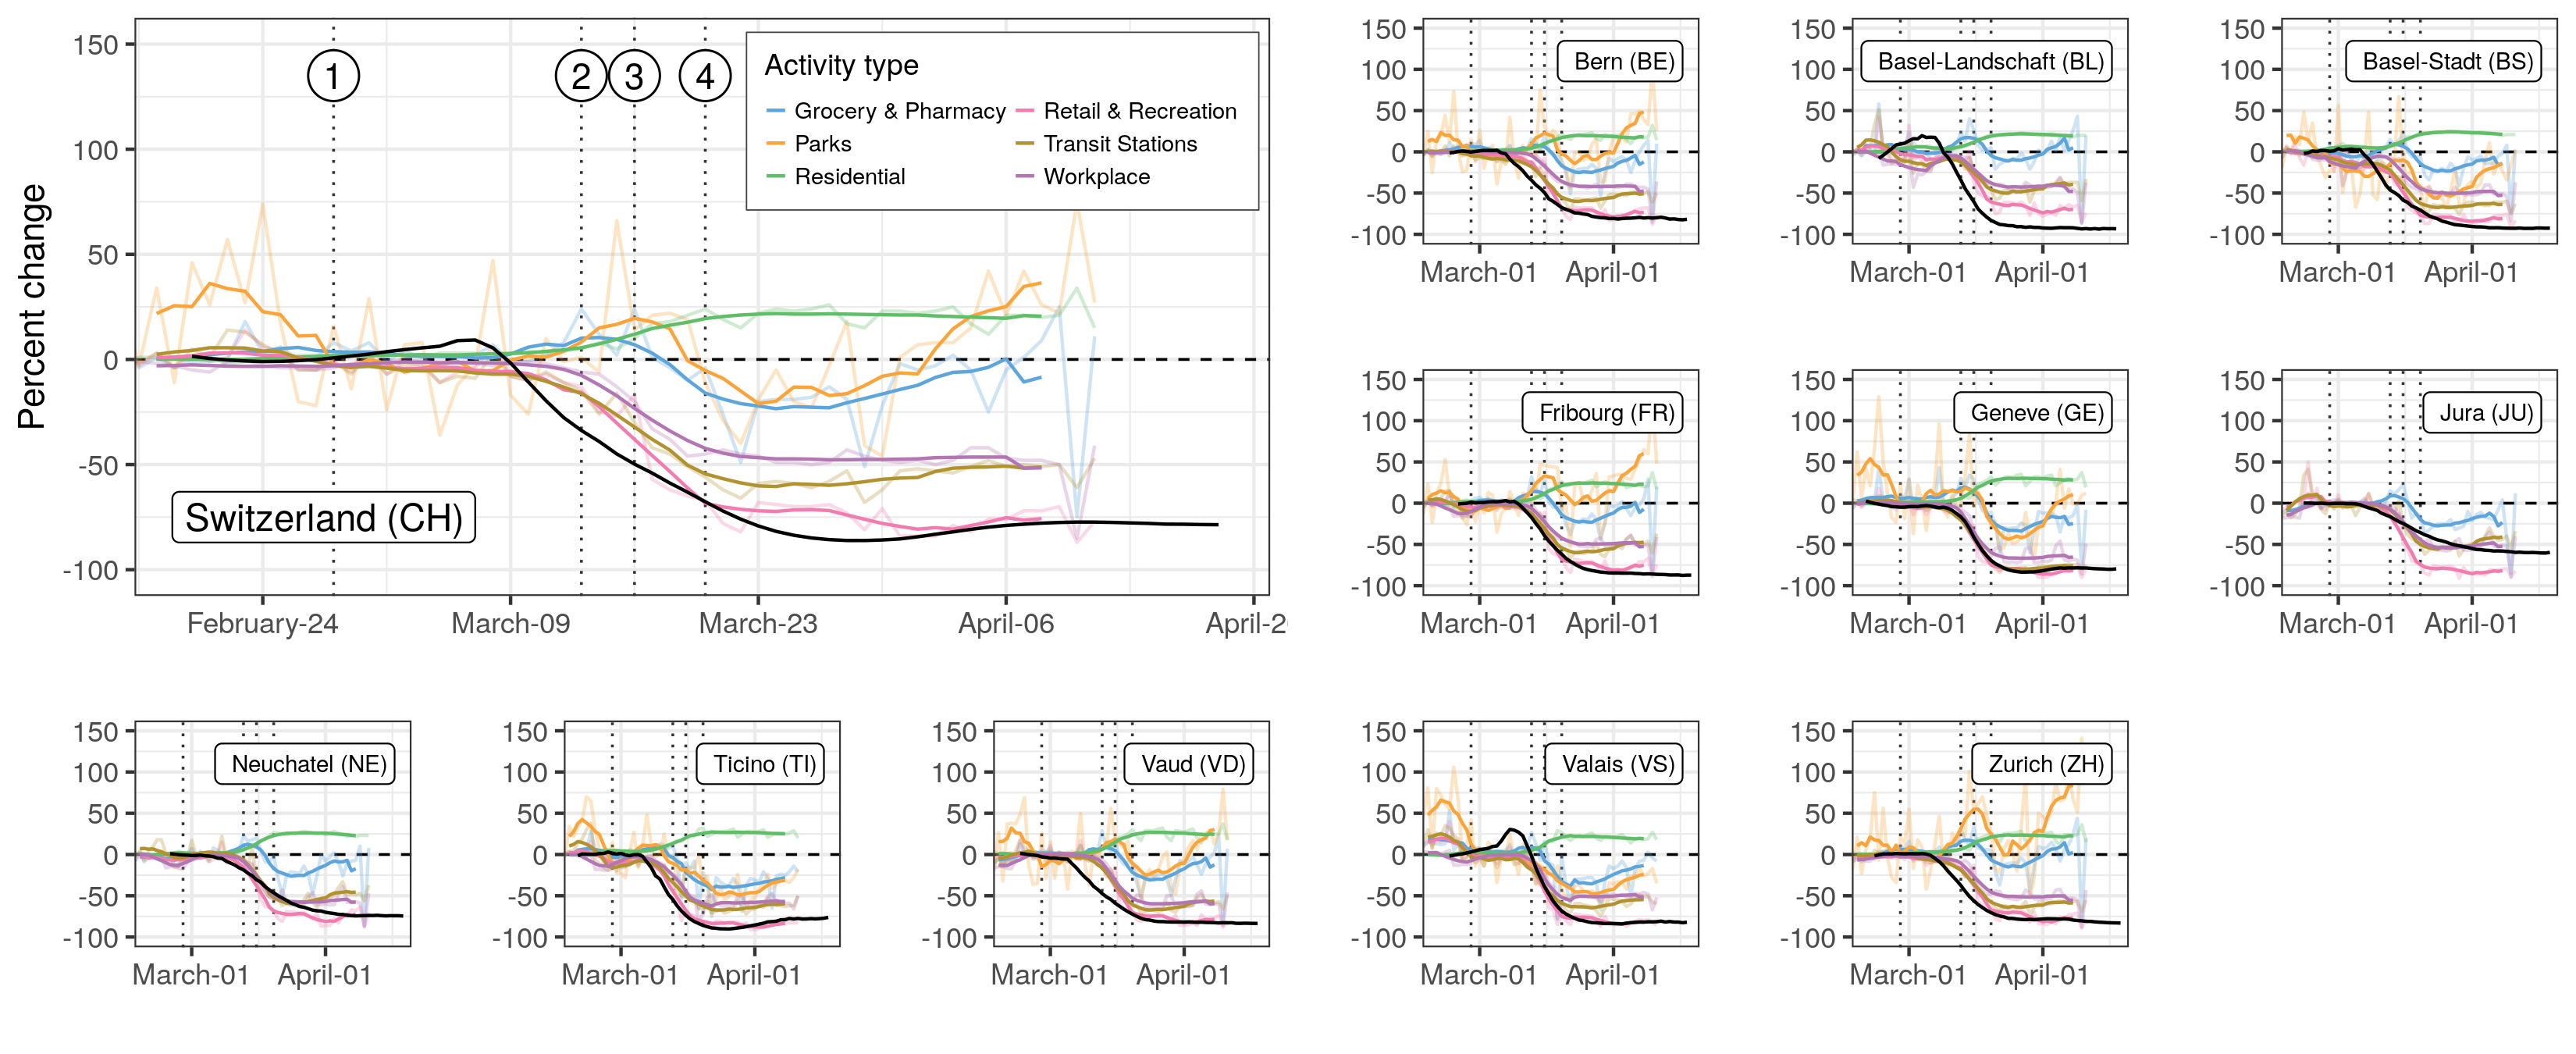
\includegraphics{fig_covid-switzerland-npi/FIGURE_3.png}
  \caption[Changes in mobility patterns and $R_0$][-1\baselineskip]{Changes in mobility patterns and $R_0$.Changes in mobility with respect to baseline are shown by activity type in terms of the daily values (transparent lines) and 7-day rolling mean (full lines), against the median estimate of $R_0$ (black line). Vertical dotted lines indicate the issuing of NPIs as described in fig.~\ref{fig:covid-ch-data}.}
  \label{fig:covid-ch-mobility}
\end{figure*}

Activity-related mobility patterns changed markedly in all cantons since the beginning of the epidemic (fig.~\ref{fig:covid-ch-mobility}). Mobility related to work, retail and recreation, and transit stations dropped by 50\% to 75\% at the national level, with cantonal-level reductions ranging from 30\% to 80\% depending on activities. Residential-related mobility increased across cantons between 20\% and 30\%. Strong support is found for mobility changes starting simultaneously for all activity types within each canton. Changes in mobility are estimated to have started between March 6 to 14 for all cantons (postprint \textsc{si} fig. 12), thus finding strong support for changes starting before school closure on March 13 (national-level mean probability across activities 0.70, cantonal range 0.55–0.99). 

Based on the changepoint models, reductions in $R_0$ likely started (probability 0.76) before observed reductions in mobility at the national level and across cantons (fig.~\ref{fig:covid-ch-mobility}). Changes in $R_0$ were highly correlated with changes in mobility, the strongest associations being with mobility related to work, transit stations, retail and recreation, and residential (cross-correlations >0.9 in all cantons and nationally, fig.~\ref{fig:covid-ch-timing}). 
\begin{figure*}\centering
  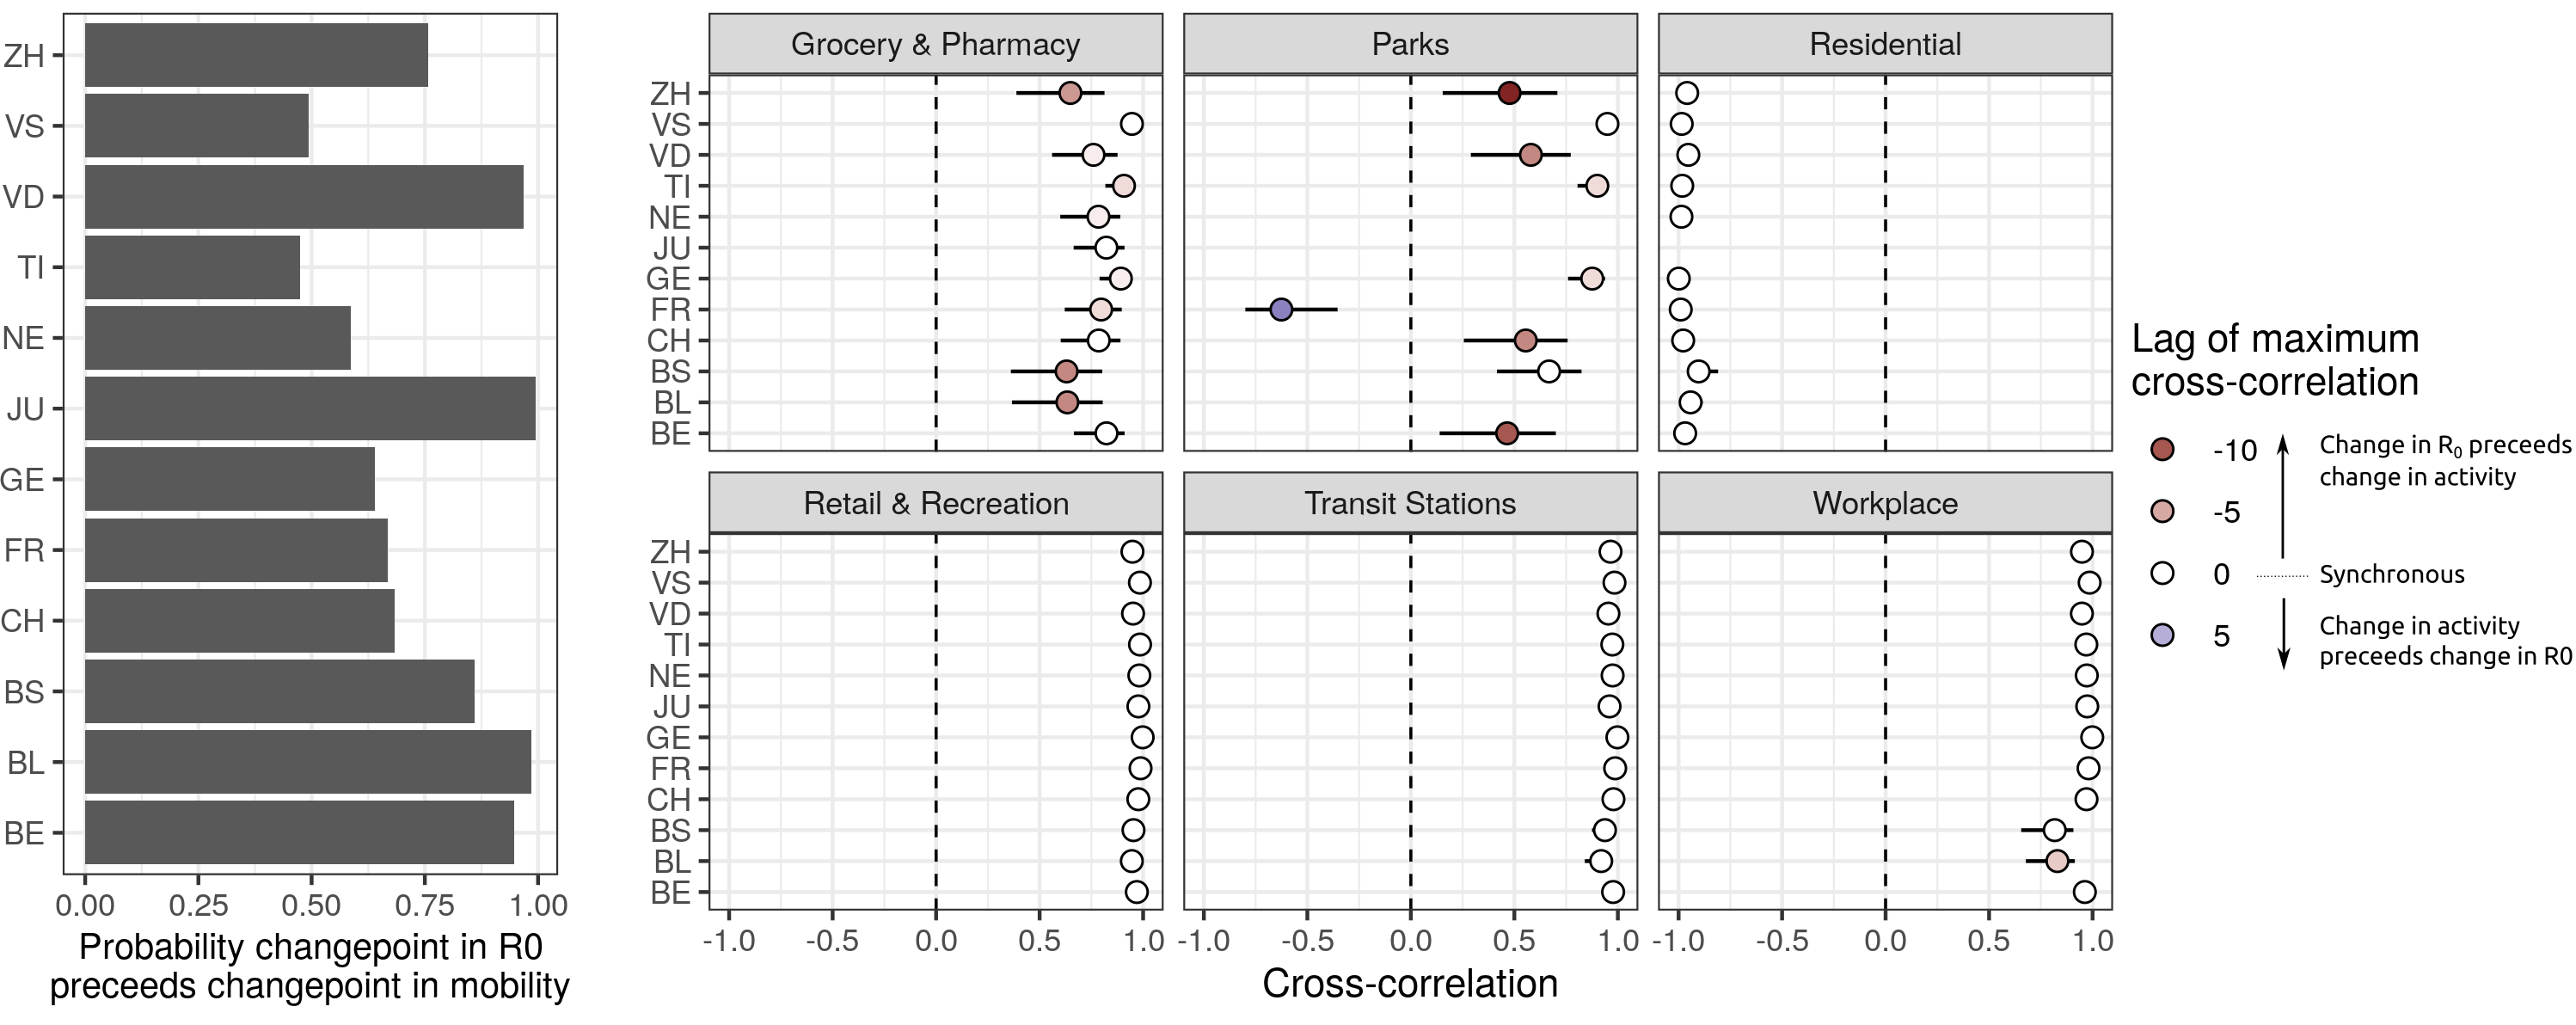
\includegraphics[width=\textwidth]{fig_covid-switzerland-npi/FIGURE_4.png}
  \caption[Timing between changes in $R_0$ and mobility][-2\baselineskip]{Timing between changes in $R_0$ and mobility. Left: probability that the first changepoint in $R_0$ occured before the first changepoint in mobility-related activity. Right: Maximum cross-correlations between time series of changes in $R_0$ and changes in mobility (bars 95\% CI). Lags refer to the delay between changes in mobility-related activity and changes in $R_0$ (positive lag k indicates that current changes in mobility have maximal cross-correlation with changes in $R_0$ $k$ days in the past).}
  \label{fig:covid-ch-timing}
\end{figure*}
In the majority of cases, correlation between mobility and $R_0$ was strongest with no lag between the two. However, changes in mobility to workplaces lagged behind changes in $R_0$ in Basel-Stadt and Basel-Landschaft. Correlations between changes in $R_0$ and grocery and pharmacy mobility were less marked (national level 0.65), with changes in mobility occurring after changes in $R_0$ (negative lags in fig.~\ref{fig:covid-ch-timing}). In most cantons, a strong increase in park mobility after March 25 resulted in a positive correlation with changes in $R_0$, but with negative lags (change in activity after change in $R_0$, fig.~\ref{fig:covid-ch-timing}). 
The linear associations between the level of reduction in mobility and maximum reduction in $R_0$ across cantons was found to be not significant, except for a small effect size for reduced park mobility (regression coefficient of 0.15, 95\% CI 0.02–0.25) (postprint \textsc{si} fig. 8). 

The effective reproduction number $R_{eff}$, a common mesure which is an aggregate measure of transmission capturing aspects of both infectious contacts and of population susceptibility was estimated. Across cantons, $R_{eff}$ was extremely close to $R_0$, indicating that a small fraction of the population is expected to have natural immunity to SARS-CoV-2. 
As of April 24, an estimated 3.9\% (95\% QR 3.6–4.3\%) of the population nationally had been infected, with median estimates ranging from 1.9\% (Bern) to 16\% (Ticino) (fig.~\ref{fig:covid-ch-map}). 
Modelled estimates of the proportion infected of people infected in the canton of Geneva are in agreement with preliminary results from ongoing serological studies, which have estimated the seroprevalence to be 9.7\% (95\% CrI 6.1–13.1\%) in the third week of April\cite[-3\baselineskip]{Stringhini:RepeatedSeroprevalenceAntiSARSCoV2:2020}, compared with modeled estimates of 8.9\% (95\% QR 7.8–10.1\%) after accounting for the time from infection to seroconversion\cite{Wolfel:VirologicalAssessmentHospitalized:2020}(postprint \textsc{si} fig. 7).

\begin{figure}\centering
  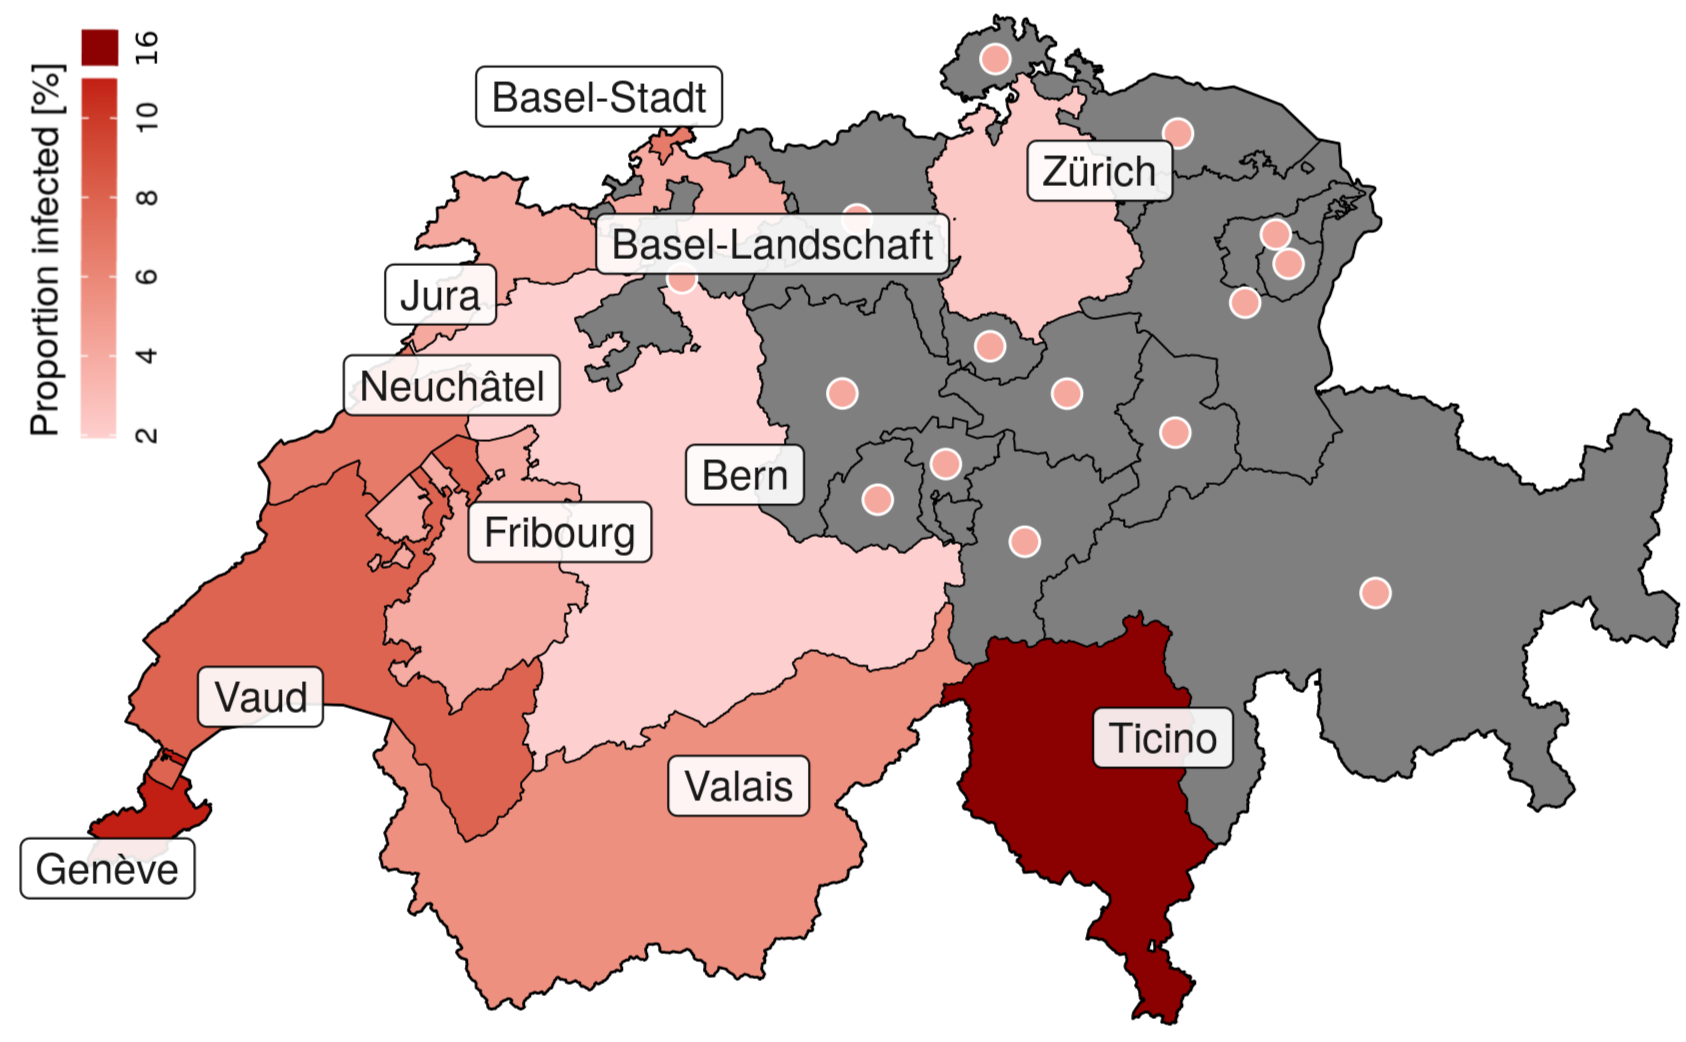
\includegraphics[width=\textwidth]{fig_covid-switzerland-npi/FIGURE_5_mod.png}
  \caption[Modelled proportion of people infected with SARS-CoV-2 in Switzerland][2\baselineskip]{Modelled proportion of people infected with SARS-CoV-2 in Switzerland up to April 24. Estimates were produced for 11 of 26 cantons for which enough data were available (unmodelled cantons are shown in gray with points indicating the national-level estimated incidence proportion of 3\%). Values are reported in the postprint \textsc{si} tab. 6.}
  \label{fig:covid-ch-map}
\end{figure}

\section{Discussion}
Our results suggest a strong reduction of $R_0$ across Switzerland since the start of the epidemic. The reduction in $R_0$ started around March 7, thus about 1 week before the implementation of lockdown-type NPIs. Analysis of activity-related mobility data also showed strong support for changes in mobility starting prior to the implementation of most NPIs. Estimated reductions of viral transmission were strongly correlated and mostly synchronous with observed changes in mobility patterns, although the initiation of changes in transmission preceded measurable changes in activity-related mobility. 

The methods used to infer the time series of $R_0$ do not rely on assumptions on the shape of how it changed in time, nor on the dates at which change started. Alternative methods that rely on fixed dates (such as that of the Imperial College \textsc{covid}-19 Response Team\cite[-6\baselineskip]{Flaxman:Report13Estimating:2020}) might be biased as changes in transmission are not synchronous with policy changes. Distribution based methods such as provided by R package EpiEstim\cite[-4\baselineskip]{Wallinga:DifferentEpidemicCurves:2004,Cori:NewFrameworkSoftware:2013} are flexible but subject to bias when misused\cite{Lipsitch:CommentPanLiu:2020}. In addition, the present approach enables the estimation of $R_0$, which is a direct quantification of transmission potential, as opposed to the effective reproduction number $R_{eff}$, which also accounts for the effect of susceptible depletion as done in the above-mentioned statistical approaches. This enabled us to estimate the proportion of reduction in transmission attribuable to behavioural changes, which is therefore more suited to study the impact of NPIs. Aside from these methodological differences, the present estimates are in line with other estimates in Switzerland: Althaus et al.\cite{Althaus:RealtimeModelingProjections:2020} estimated a reduction of 89 \% (83–94\%) from a baseline of 2.78 (2.51–3.11), Scire et al.\cite{Scire:ReproductiveNumberCOVID19:2020} estimated a reduction of 76 \% (70–82\%) from a baseline of 1.88 (1.80–1.98) and Imperial College estimated a reduction of 60\% (50–80\%) from a baseline of 3.5 (2.8–4.3)\cite{Flaxman:Report13Estimating:2020}. 

The presented results provide strong support for a reduction of transmission starting about 1 week prior to school closure, the first national-level NPI targeting daily activities, which was ordered on March 13. Moreover, initiation of transmission reduction was found to precede changes in mobility patterns as detectable from the Google dataset. A possible explanation for this initial decrease in transmission could be linked to the strong increase in public interest in \textsc{covid}-19 in February as measured by Google searches for \textsc{covid}-19-related keywords (fig.~\ref{fig:googlemob}).
\begin{marginfigure}[1\baselineskip]
%\centering
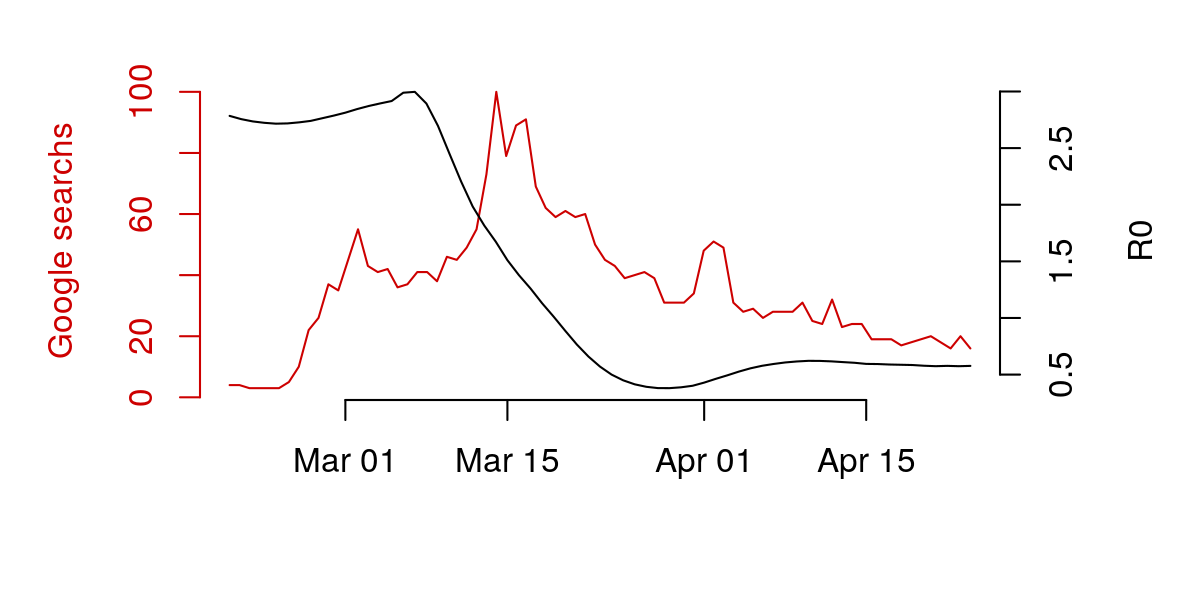
\includegraphics{fig_covid-switzerland-npi/fig_supp/google_trends.png}
\margincaption[Google trends for \textsc{covid}-19 and changes in R$_0$ in Switzerland]{\footnotesize Google trends for \textsc{covid}-19 and changes in R$_0$ in Switzerland. Trends corresponds to amount of searches for the keyword "coronavirus" (red line) between February 15 and April 30 and are given as a percent of the maximum number of searches in the period, time evolution of R$_0$.}\label{fig:googlemob}
\end{marginfigure}
 In fact, a second sharp rise in Google searches is estimated to have started on March 7 (95\% CrI March 3–9), which overlaps with the estimated start of national level decrease in $R_0$ on March 7 (probability that changepoints coincide 0.76). The Federal Office for Public Health issued an information campaign on \textsc{covid}-19 on February 28, which was updated on March 2 to stress basic hygiene rules\cite{OFSP:NouvellesReglesHygiene:2020}. This may have resulted in voluntary social distancing as well as increased hygiene early on without noticeable changes in mobility patterns. This type of proactive change in behaviour would be in line with early changes in mobility patterns, which were estimated to precede school closures and subsequent measures. The present results suggest that the value of $R_0$ was likely already below one on March 20, when the federal government banned gatherings of more than five people and recommended voluntary home isolation for the whole population. This result should however be taken within context, as the announcement was anticipated on social networks earlier that week, and so was probably already impacting social distancing behaviour. 
Therefore caution is recommend in any causal interpretation of these results on the role of this last NPI on driving $R_0$ below one.

Despite the strong association between the changes in mobility and reductions in $R_0$ within each canton, the lack of cross-cantonal associations between the level of reduction in mobility types and the level of reduction in $R_0$ suggests context-specific pathways between \textsc{covid}-19 transmission and mobility intensity. This warrants caution in attempting to apply general relations between mobility and transmission reduction. Investigation of general associations will require more in-depth studies controlling for other factors such as population density, economic activities and social mixing patterns, and inter-cantonal mobility patterns, in addition to incorporation of potential environmental drivers of transmission such as temperature and relative humidity\cite{Neher:PotentialImpactSeasonal:2020, Kissler:ProjectingTransmissionDynamics:2020}. 
  
  Several limitations to this work are noted. First, due to the relatively recent introduction of SARS-CoV-2 in Switzerland compared with the length of hospital and ICU stays, the time distribution of hospital in- and out-patients is biased towards shorter duration (see \textsc{Appendix}), which is addressed by accounting with right-censoring using survival models. In addition, because of the limited data available in some places, it was only possible to fit the model for 11 of the 26 cantons. Modelling results presented in this work are subject to hypothesis on yet uncertain parameters of \textsc{covid}-19, including the infection fatality rate and the proportion of severe infections requiring hospitalisation. An important uncertainty is the fraction of asymptomatic infections and their relative contribution to disease transmission. It is assumed that all infected individuals contribute equally to transmission, which means the estimation of the proportion of people infected would under-estimate true cumulative incidence if there were a large fraction of asymptomatic infections with a relatively low contribution to transmission. Evidence from South Korea, however, suggests that only a small fraction (2\%) of confirmed \textsc{covid}-19 infections are totally asymptomatic, and none of the household members of these asymptomatic carriers were infected\cite[-4\baselineskip]{Park:EarlyReleaseCoronavirus:2020}. Moreover, model results are in agreement with preliminary results from ongoing serological studies in Switzerland\cite[-2\baselineskip]{Stringhini:RepeatedSeroprevalenceAntiSARSCoV2:2020}.  The presented estimates of time-varying basic reproduction numbers assume that the generation interval for \textsc{covid}-19 in Switzerland remained unchanged, thus potentially ignoring the joint role of $R_0$, the infectious period and contact rates in determining the disease’s intrinsic growth rate\cite{Yan:SeparateRolesLatent:2008}. If the generation interval increased with the reduction of social contact then these estimates are conservative overestimates of the “true” value of $R_0$, which is encouraging from a public health perspective. Inferred disease dynamics and estimated time-varying $R_0$ also depend on the values of the incubation period, which is set to the estimates currently available in the literature. 
  In the present modelling framework, the initial conditions were estimated along with changes in $R_0$, which could, however, be influenced by the role of imported cases in driving disease dynamics, especially in cantons bordering regions with strong \textsc{covid}-19 transmission in early February (Eastern France for Basel-Stadt and Basel-Landschaft and Northern Italy for Ticino). 
  Since importations were not modeled, this could yield an overestimation of the initial value of $R_0$, which warrants caution in interpreting specific values of $R_0$ in these cantons. This potential overestimation would, however, not affect the strong inferred reduction in $R_0$. Another limitation of this study is that it was not possible to disentangle the individual contribution of each NPI on $R_0$ in this analysis owing to the early onset of changes in $R_0$ and in mobility patterns, as well as the very close spacing between the different types of NPI. This information would, however, be extremely valuable in supporting decisions on NPI strategies against \textsc{covid}-19. Efforts to constitute a global database of NPIs will provide the opportunity to extend this type of analysis to other settings and produce evidence for the effect of different types of NPIs\cite{HITCOVIDTeam:HealthInterventionsTracking:2020}. 
  
  As the Swiss government plans to gradually lift restrictions, close monitoring of changes in $R_0$ is critical, given that the reductions in transmission appear to be almost entirely driven by changes in behaviour, not through herd immunity. Near real-time estimates of $R_0$ may serve as a critical tool for public health and political decision makers in the months to come, and efforts should be made to refine models like ours using new data, including those from population-based serological studies, mobility data and more detailed individual-level data on \textsc{covid}-19 cases across the spectrum of severity.\marginnote[-4\baselineskip]{While relying on hospitalization and death allowed for an early robust identification of the basic reproduction number, it would be necessary to add a reporting process and case data to update this estimate through 2020-2021. Methods based on observed data are easier to maintain, and reliable continuous updates of the reproduction number in Switzerland available on the Swiss National \textsc{covid}-19 Task Force website \url{sciencetaskforce.ch/en/current-situation/}. It is provided by the ETHZ, with method described in \fullcite{Huisman:EstimationWorldwideMonitoring:2021}. The modeled incidence from the present Chapter has been later used as "truth" to compare waste-water data with reported cases, see: \fullcite{Fernandez-Cassi:WastewaterMonitoringOutperforms:2021}.}

 % 5
%\begin{fullwidth}
	\chapter[Optimizing the spatio-temporal allocation of  covid-19 vaccines: Italy as a case study]{Optimizing the spatio-temporal allocation of \\covid-19 vaccines: Italy as a case study}
\label{ch:covid-italy-ocp}

The development of vaccines has sparked high hopes towards the control of SARS-CoV-2 transmission without resorting to extensive community-wide restrictions. A fundamental question concerns the best possible allocation of a limited vaccine stock in space and time given a specific goal. In this chapter, this is addressed through an optimal control framework based on a spatially explicit COVID-19 epidemiological model \parencite{Bertuzzo:GeographyCOVID19Spread:2020,Gatto:SpreadDynamicsCOVID19:2020}, where vaccine distribution is optimized under supply and deployment capacity constraints. This tool provides strategies for optimal allocations in different scenarios, yielding important improvements over considered alternatives. By accounting for spatial heterogeneities and human mobility networks, the presented approach complements currently used allocation methods based on criteria such as age or risk.
This chapter is based on the following preprint: \longfullcite{Lemaitre:OptimizingSpatiotemporalAllocation:2021}

\section{Abstract}
While SARS-CoV-2 vaccine distribution campaigns are underway across the world, communities face the challenge of a fair and effective distribution of limited supplies. One may wonder whether suitable spatial allocation strategies might significantly improve a campaign's efficacy in averting damaging outcomes. To that end, the problem of optimal control of COVID-19 vaccinations is addressed in a country-wide geographic and epidemiological context characterized by strong spatial heterogeneities in transmission rate and disease history. The vaccine allocation strategies in space and time that minimize the number of infections in a prescribed time horizon are searched for. Scenarios of unfolding disease transmission across the 107 provinces of Italy, from January to April 2021, are generated by a spatially explicit compartmental COVID-19 model tailored to the Italian geographic and epidemiological context. A novel optimal control framework is developed to derive optimal vaccination strategies given the epidemiological projections and constraints on vaccine supply and distribution logistic. Optimal schemes significantly outperform simple alternative allocation strategies based on incidence, population distribution, or prevalence of susceptibles in each province. Results suggest that the complex interplay between the mobility network and the spatial heterogeneities imply highly non-trivial prioritization of local vaccination campaigns. The extent of the overall improvements in the objectives grants further inquiry aimed at refining other possibly relevant factors so far neglected. This \textsc{Chapter} thus provides a proof-of-concept of the potential of optimal control for complex and heterogeneous epidemiological contexts at country, and possibly global, scales.
% stuff removed: provide a benchmark for decision maker.
% Please keep the Author Summary between 150 and 200 words
% Use first person. PLOS ONE authors please skip this step. 
% Author Summary not valid for PLOS ONE submissions.   
\end{fullwidth}

%% ***********************************************************************************************
\section{Introduction}
%% ***********************************************************************************************
% opening 
Supply- or deployment-limited SARS-CoV-2 vaccines\cite[-2\baselineskip]{Khamsi:IfCoronavirusVaccine:2020} pose the urgent question of a fair distribution of the available doses\cite[-1\baselineskip]{NationalAcademiesofSciencesEngineeringandMedicine:FrameworkEquitableAllocation:2020}. Current prioritization approaches typically target groups at higher risk of severe outcomes\cite{Spassiani:VaccinationCriteriaBased:2020, Matrajt:VaccineOptimizationCOVID19:2020a}, or their indirect protection by vaccinating those with higher disease transmission\cite{%Spassiani:VaccinationCriteriaBased:2020,
Gallagher:IndirectBenefitsAre:2021,Tuite:AlternativeDoseAllocation:2021}. Our main hypothesis is that taking into account spatial heterogeneities in disease transmission when designing prioritization strategies will significantly improve the effectiveness of vaccination campaigns.
%Model-informed studies\cite{bubar_model-informed_2021} investigate prioritization plans by exploring the effects of the suitable removals of vaccinated individuals from the pool of susceptibles within the context of unfolding disease transmission. 
The distribution of doses inside each country is limited by the logistic capabilities of the healthcare network and the rate at which the vaccine stock is replenished. Decisions concerning the best allocation strategies are to be taken under these constraints. Moreover, both the complex coupling between regions due to human mobility and the spatial heterogeneities in disease history and control interventions make the discovery of such optimal allocation strategies an arduous task.

An optimal control framework to explore COVID-19 vaccine distribution in space and time is proposed.
%employing a spatially explicit disease transmission model\cite{Gatto:SpreadDynamicsCOVID19:2020,Bertuzzo:GeographyCOVID19Spread:2020}. It allows us to design optimal vaccine allocation strategies meeting constraints on vaccine distribution or supply in a automated manner.    
%posit that is that suboptimal choices on the allocation of vaccines may significantly worsen the outcomes of the epidemic in a specific geographical and epidemiological context.
The SARS-CoV-2 epidemic in Italy is studied, where strong spatial effects arise from the geography of the disease, heterogeneous lockdown exit strategies, and post-lockdown control measures\cite[-4.5\baselineskip]{Marziano:RetrospectiveAnalysisItalian:2021}. The optimal control framework is applied to a spatial model that has proved its reliability for Italy%\cite[-5\baselineskip]{Gatto:SpreadDynamicsCOVID19:2020,Bertuzzo:GeographyCOVID19Spread:2020}
, updated through data assimilation of a year-long epidemiological record. This allows us to unravel the best possible vaccination strategy and probe the impact of vaccine allocations over the 107 Italian provinces.

%knowledge gap
The problem of vaccine allocation is of primary importance for  public-health officials, epidemiologists, and economists\cite[-7.5\baselineskip]{Emanuel:EthicalFrameworkGlobal:2020, Lipsitch:UnderstandingCOVID19Vaccine:2020}. 
Roll-out strategies are conventionally based on the prioritization of individuals at risk, such as health workers and elderly people\cite[-6.5\baselineskip]{Bubar:ModelinformedCOVID19Vaccine:2021,Fitzpatrick:OptimizingAgespecificVaccination:2021,Baden:EfficacySafetyMRNA1273:2020,Yang:WhoShouldBe:2021}. However, the heterogeneous ways in which different regions may be affected by each successive wave raise questions about spatial prioritization strategies. What is the best feasible spatial allocation, given supply and logistic constraints? Would that differ significantly from current non geographically-optimized plans? Should vaccines be distributed on the basis of demography or would it be better to prioritize areas currently subject to an outbreak? How relevant are the susceptibility profile and modelled future transmission in each region? 
%How well performs this optimal strategy against e.g a uniform allocation ?

% lit review
Epidemiological modeling has long been used to answer questions about the impact of vaccination campaigns, often by comparing outcomes under different scenarios\footnote[][-9.3\baselineskip]{such as the study by \textcite{Lee:AchievingCoordinatedNational:2020} presented in \textsc{Chapter 5}}. Optimization, i.e, the search for the best possible course of action that maximizes or minimizes an objective metric, has been carried out theoretically since the seventies\shortcite[-10\baselineskip]{Morton:OptimalControlDeterministic:1974,Sethi:OptimalControlSimple:1978, Greenhalgh:ResultsOptimalControl:1988}. Recent dramatic improvements of both algorithms\cite[-8.5\baselineskip]{Quirynen:MultipleShootingMicrosecond:2015} and computational power prompted applied studies using different methods to rigorously find optimal mitigation strategies: most of the time trough iterative parameter search\shortcite[-10\baselineskip]{Sah:OptimizingImpactLowefficacy:2018, Medlock:OptimizingInfluenzaVaccine:2009}, but also using genetic algorithms\shortcite[-9\baselineskip]{Patel:FindingOptimalVaccination:2005} or solving the Hamilton-Jacobi-Bellman equations\shortcite[-9\baselineskip]{Zakary:AnalysisMultiregionsDiscrete:2017, MillerNeilan:OptimalVaccineDistribution:2011}.

Interesting developments have recently arose during the ongoing SARS-CoV-2 pandemic\cite[-10\baselineskip]{Fitzpatrick:OptimizingAgespecificVaccination:2021, Thul:StochasticOptimizationVaccine:2021,Moore:VaccinationNonPharmaceuticalInterventions:2021}. The urgency of effective vaccination campaigns led to the development of modeling frameworks for the optimization of vaccine allocation, based on age or risk\shortcite[-6\baselineskip]{Matrajt:VaccineOptimizationCOVID19:2020a,Spassiani:VaccinationCriteriaBased:2020,Fitzpatrick:OptimizingAgespecificVaccination:2021, Bubar:ModelinformedCOVID19Vaccine:2021}, dose timing\cite[-4\baselineskip]{Saad-Roy:EpidemiologicalEvolutionaryConsiderations:2021, Kadire:DelayedSecondDose:2021}, and the deployment of testing resources, using optimal control\cite{Acemoglu:OptimalAdaptiveTesting:2021} or Bayesian experimental design\cite{Chatzimanolakis:OptimalAllocationLimited:2020}, along with prioritization based on social contact networks\cite{Chen:PrioritizingAllocationCOVID19:2021}. 

To our knowledge, optimal spatial allocation of COVID-19 vaccines at a country scale has never been performed yet. This question is distinct from, and complementary to, risk-based prioritization. Spatial heterogeneities in disease transmission are complex, as seen during the initial outbreaks%\cite{Li:SubstantialUndocumentedInfection:2020}
, supporting the significance of the posed problem towards an effective control of the epidemic. However, the connectivity network underlying spatial epidemiological models may generate complex large-scale control problems whose solution requires tailored formulations and efficient algorithms.  

% Description:intro
This work aims to find optimal strategies for this problem through modern optimization methods based on distributed direct multiple shooting, automatic-differentiation, and large-scale nonlinear programming\cite{Bock:MultipleShootingAlgorithm:1984,Savorgnan:MultipleShootingDistributed:2011,Andersson:CasADiSoftwareFramework:2018,Wachter:ImplementationInteriorpointFilter:2006}. This allows us to solve the large-scale optimization problems arising from epidemiological models, even when considering hundreds of spatial nodes. 


%% ***********************************************************************************************
\section{Materials and methods} \label{sec:matmet}
%% ***********************************************************************************************

The formulation of the optimal control problem has three main components: 1) an objective function to be minimized, here the total incidence in Italy from January 11, 2021 to April 11, 2021; 2) the set of constraints that the control must satisfy, in our case the limitations on vaccine administration rate in each province and the total vaccine stock in Italy; and 3) the spatial epidemiological model\cite{Gatto:SpreadDynamicsCOVID19:2020, Bertuzzo:GeographyCOVID19Spread:2020} governing the transmission dynamics with the daily vaccination rates in each province as control variables.

The objective, the model, and the constraints may be tailored to specific applications within the proposed framework.

% Description:objective
\subsection{Objective function.} Optimizing calls for a metric, whose selection is critical in determining the optimal solution and its outcome. The choice of an objective function relates health, economy, and ethics. Possible candidates are the minimization of e.g.~DALYs (the Disability-Adjusted Life Years), the number of deaths, and economic loss\cite{Du:ComparativeCosteffectivenessSARSCoV2:2021}. All these objectives are linked and may be combined together. As the model considered for this work does not have risk-classes, without loss of generality it is optimized for the minimization of the incidence on Italy from January 11, 2021 to April 11, 2021. Minimization of the deaths would yield the same results under the assumptions the model used.

% Description:constraints
\subsection{Constraints} Two types of constraints are defined: supply constraints, which determine the weekly delivery to the national stockpile; and logistic constraints, which limits the maximum rate of local vaccine distribution in each province.

The supply constraints ensure that the model does not distribute more vaccine than what is actually available in stock. It is assumed that the national supply of vaccine doses is empty on January 11, 2021 and is replenished every Monday. Four scenarios are considered with weekly deliveries of 479'700 (realistic, baseline value), 1M, 1.5M and 2M vaccine doses.

From the national stockpile, doses may be allocated to any of the 107 Italian provinces, but the logistic constraints limit the rate at which it is possible to distribute the vaccines in each province. The maximum number of individuals who can be vaccinated in a province per day is assumed to be proportional to the province's population, such that the national maximum distribution capacity equals 500,000 doses per day, i.e., 3.5M per week if every province vaccinates at its maximum rate (which in retrospect is close to Italy's vaccination rate as of May 1st). 

\begin{figure}[!ht]
    \centering
    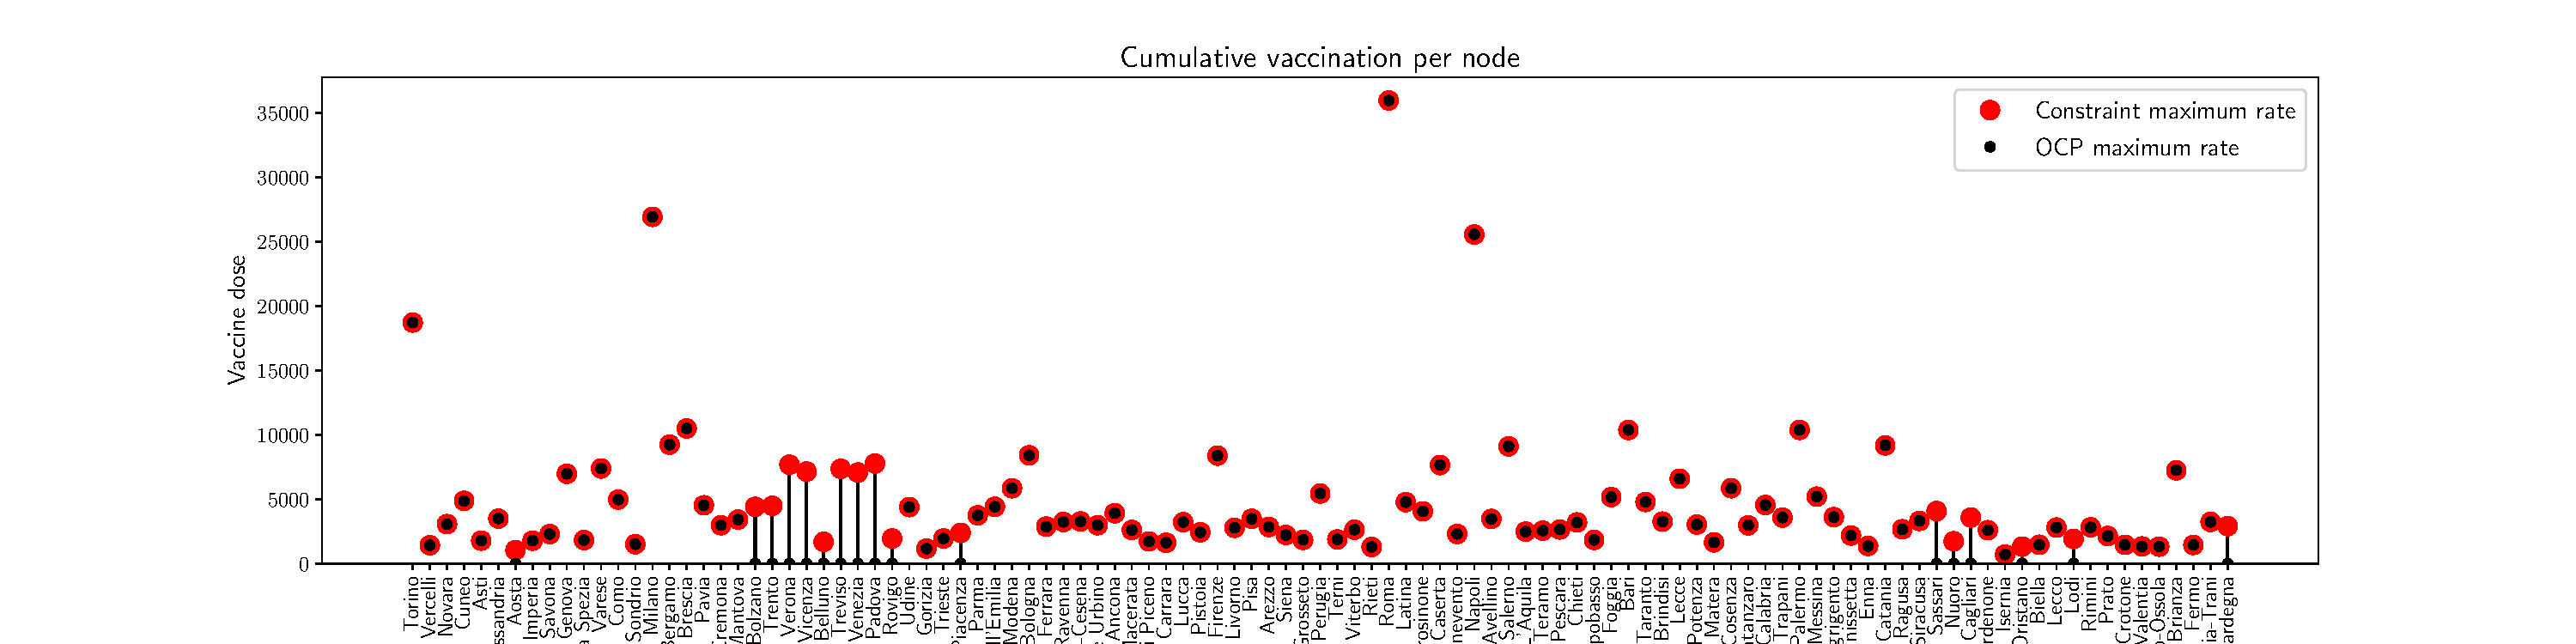
\includegraphics{fig_italy-ocp/figuresSI/SI_constraint_dist.pdf}
    \caption[Vizualisation of the local maximum vaccination rate constraint][-2\baselineskip]{Local maximum vaccination rate constraint $v_i^\mathrm{max}$ for each province. This logistic constraint bounds the maximum number of vaccines to 0.5M of doses per day, with a local rate that is proportional to the node population. Here the maximum vaccination rate for each province (the constraint the solution has to comply with) is shown in red, and the maximum rate prescribed by the optimal solution while simulating the pessimistic scenario with a stockpile delivery of 479'700 doses, in black. The optimal solution uses the maximal capacity of the logistic network, while respecting the constraint defined.}
    \label{fig:OC_logistic_constraints}
\end{figure}


 % Description:model
\subsection{Epidemiological model.} 
The optimal control framework may be used with any compartmental SARS-CoV-2 transmission model that can be approximated by ordinary differential equations. To demonstrate its usefulness, it is applied a complex model based on previous work that was aimed to describe the first wave of COVID-19 infections in Italy\parencite{Gatto:SpreadDynamicsCOVID19:2020,Bertuzzo:GeographyCOVID19Spread:2020}. 
%Incidence and deaths are projected using the spatially distributed epidemiological model devised by Gatto et \textit{al.}\cite{Gatto:SpreadDynamicsCOVID19:2020} and further improved by Bertuzzo et \textit{al.}\cite{Bertuzzo:GeographyCOVID19Spread:2020}. 

The proposed framework is constituted of two disease transmission models, one "true" model and a simplified one used for control:
\begin{itemize}
    \item The full model is a COVID-19 model, as designed in\cite{Gatto:SpreadDynamicsCOVID19:2020, Bertuzzo:GeographyCOVID19Spread:2020}. This model is ODE-based, includes full connectivity based on mobility data, and is implemented in MATLAB using the adaptive step ode45 integration scheme. Using data assimilation, the joint-posterior distribution is obtained for all parameters of this model. 
    \item The simplified model used for optimal control is an approximation of the above model, integrated using an explicit Runge-Kutta 4 method with fixed stepsize. The problem is simplified by limiting the connectivity to the largest mobility fluxes (see fig.~\ref{fig:model_description_network} and optimizing only one realization of the posterior. This model is implemented in Python with the CasADi library.
\end{itemize}

\paragraph{Model description}
The model subdivides the Italian population into its 107 provinces represented as a network of connected nodes. Each province has local dynamics describing the number of individuals present in each of the model compartments: susceptible $S$, exposed $E$, pre-symptomatic $P$ (incubating infectious), symptomatic infectious $I$, asymptomatic infectious $A$, hospitalized $H$, quarantined $Q$, recovered $R$, and dead $D$. A tenth compartment, vaccinated individuals $V$, is added to the original nine, as shown in fig.~\ref{fig:model_description_diag}.

\begin{marginfigure}
\centering
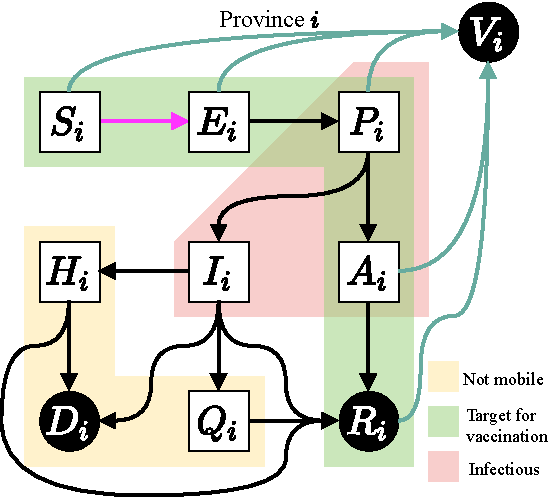
\includegraphics{fig_italy-ocp/figures/OCPItalydrawio2.pdf}
%    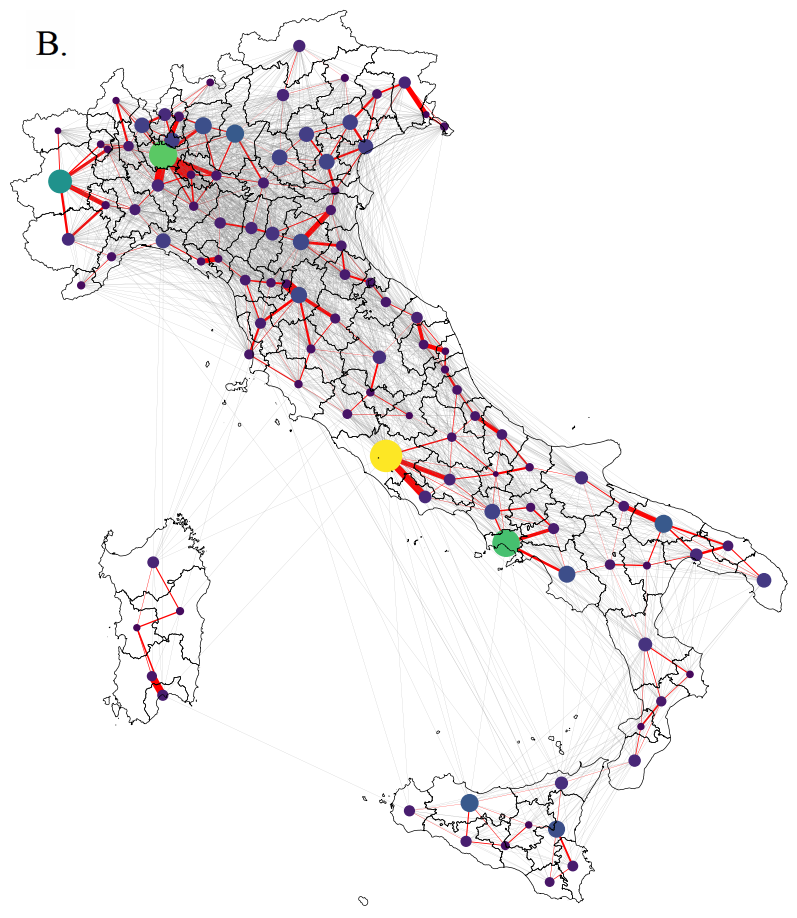
\includegraphics[width=0.40\textwidth]{fig_italy-ocp/figures/map_nd.png}
\margincaption[Optimal control model compartments diagram]{Diagram representing the compartments of the epidemiological model and the possible transitions in a single province. The control is the vaccination rate (teal arrows), aiming at minimizing incident infections (pink arrow). Individuals in compartments outside of the yellow block are able to move along the mobility network.}
    \label{fig:model_description_diag}
\end{marginfigure}


Apart from hospitalized $H$, quarantined $Q$, dead $D$, and symptomatic individuals $I$, a fraction of the other individuals commutes between provinces along the mobility network, thus node-to-node disease transmission is introduced along the network shown in fig.~\ref{fig:model_description_network}.

Compartments $P$, $A$, and $I$ have different degrees of infectiousness and contribute to the force of infection (eqn.~\eqref{eq:foiL} and \eqref{eq:foiM}), which represents the rate at which susceptibles $S$ become infected and, thus, enter the exposed compartment $E$. The force of infection in each province is constituted of a local and a mobility component. The local component describes transmission among the local individuals. The mobility component considers that local susceptibles may enter in contact with infected individuals that are traveling, and oppositely, susceptible commuters may become infected through contact with local infected. Connected provinces contribute to this process depending on the strength of the mobility fluxes from and to the node of interest.

The estimated vaccine efficacy and immunity duration depends on the vaccine type. Because the focus is on spatial patterns and differences among vaccination strategies, the vaccination process is simplifed by assuming a one-dose vaccine with instantaneous 100\% efficacy. %This simplification does not influence the relative vaccine allocation between provinces and is independent of the specific vaccine used. 
Moreover, that vaccines protection is assume persists during the three months of projection considered.

In the end, the COVID-19 transmission dynamics are described by the following set of ordinary differential equations in each node $i$: 
\begin{equation}\label{eq:sepiar}
\begin{split}
    \dot{S}_i &= - \lambda_i(t) S_i - r^v_i(t) S_i \\
    \dot{E}_i &= \lambda_i(t) S_i -  (\delta^E + r^v_i(t)) E_i \\
    \dot{P}_i &= \delta^E E_i -  (\delta^P+r^v_i(t))  P_i \\
    \dot{I}_i &= \sigma \delta^P P_i - (\gamma^I + \eta)  I_i \\
    \dot{A}_i &= (1 - \sigma) \delta^P P_i - (\gamma^A+ r^v_i(t)) A_i \\
    \dot{Q}_i &= \zeta \eta I_i - \gamma^Q Q \\
    \dot{H}_i &= (1-\zeta) \eta I_i - (\gamma^H + \alpha^H)H \\
    \dot{R}_i &= \gamma^I I_i + \gamma^A A_i + \gamma^H H_i + \gamma^Q Q_i - r^v_i(t) R_i\\
    \dot{V}_i &= r^v_i(t) \cdot (S_i + E_i + P_i + A_i + R_i).
\end{split}
\end{equation}
$N_i$ the population of province $i$. Susceptible individuals get exposed to the pathogen at rate~$\lambda_i(t)$, corresponding to the force of infection for community~$i$, thus becoming latently infected (but not infectious yet). Exposed individuals transition to the post-latent, infectious stage at rate~$\delta^E$. Post-latent individuals progress to the next infectious classes at rate $\delta^P$, developing an infection that can be either symptomatic---with probability~$\sigma$---or asymptomatic---with probability $1 - \sigma$. Symptomatic infectious individuals recover from infection at rate~$\gamma^I$ and may seek treatment at rate~$\eta$. Asymptomatic individuals recover at rate~$\gamma^A$.  Infected individuals who sought treatment are either hospitalized (rate $1-\zeta$) or quarantined (rate $\zeta$) at home and are considered to be effectively removed from the community, thus not contributing to disease transmission. Individuals who recover from the infection are assumed to have long-lasting immunity to reinfection at the timescale studied, but possible loss of immunity can be easily included in the model. Hospitalized individuals die at rate $\alpha_H$ and recover at rate $\gamma^H$.

Individuals in compartments $S, E, P, A, R$ might receive vaccine doses. If the chosen strategy allocates $v_{i}(t)$ doses in node $i$ at time t, the vaccination rate is

\begin{equation}
r^v_i(t) = \frac{v_{i}(t)}{S_i(t) +  E_i(t) + P_i(t) + A_i(t) + R_i(t)}
\end{equation}

Vaccinated individuals are moved at rate $r^v_i(t)$ from their original compartments to compartment $V$, where they do not contribute to the infection anymore.

\paragraph{Force of infection and simplifications}
The force of infection of the full model is specified as in Gatto et \textit{al.}\cite[-4\baselineskip]{Gatto:SpreadDynamicsCOVID19:2020}, Bertuzzo et \textit{al.}\cite{Bertuzzo:GeographyCOVID19Spread:2020}. In addition to province's local dynamics, it also considers that local susceptibles may enter in contact with infected individuals that are traveling, and oppositely, susceptible commuters may become infected through contact with local infected. The force of infection of the OCP model slightly simplified:

The force of infection $\lambda_i(t)$ is split between the sum of the local force of infection $\lambda^L_i(t)$, from infected in node $i$ and a mobility-driven force of infection from the network $\lambda^N_i(t)$, hence $\lambda_i(t) = \lambda^L_i(t) + \lambda^M_i(t)$. While running our model, it became apparent that $\lambda^M_i(t) \ll \lambda^L_i(t)$. Hence this artificial separation will be exploited when simplifying our model. As described below, $\lambda^M_i(t)$ is updated every day whereas $\lambda^L_i(t)$ is updated at each integration step.
\begin{marginfigure}
\centering
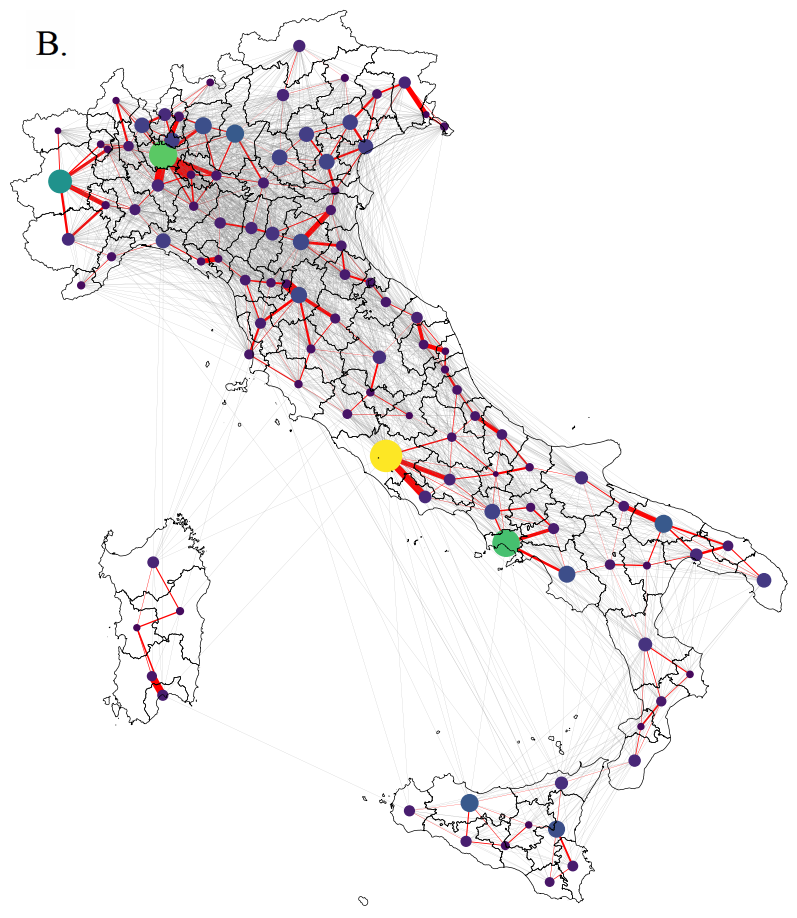
\includegraphics{fig_italy-ocp/figures/map_nd.png}
\margincaption[Optimal control mobility network]{Mobility network: the force of infection in a province is coupled to the dynamics of other connected provinces. To reduce the problem to a tractable size, only the most important connections (red edges) are considered when optimizing, but the full network (red and grey edges) is used to assess our strategies. Nodes size and color display each province's population, and edges width shows the straight of the coupling between each pair of provinces.}
    \label{fig:model_description_network}
\end{marginfigure}

As for the formulations of the force of infection, the formulas designed by \textcite{Gatto:SpreadDynamicsCOVID19:2020,Bertuzzo:GeographyCOVID19Spread:2020}are recalled here. The local force of infection reads:
\begin{equation} 
     \lambda^L_i(t) = C_{i,i} \beta_{0}  \beta_i(t) \cdot \frac{C_{i,i}  (P_i + \epsilon_A  A_i) + \epsilon_I  I_i}{C_{i,i} \cdot (S_i + E_i + P_i + R_i + A_i + V_i) + I_i}, \label{eq:foiL}
\end{equation}
and the influence of other provinces on province $i$ is written as:
\begin{equation}
     \lambda^M_i(t) = \sum_{m, m \neq i} \left( 
     C_{i,m} \cdot 
     \frac{
     \sum_{n, n \neq m} \left[ C_{n,m} \cdot \beta_{0}  \beta_n(t)  (P_n + \epsilon_A  A_n) \right] + \epsilon_I  \beta_{0}  \beta_m(t)  I_m
     }
     {
     \sum_{l, l \neq m}  \left[C_{l, m} \cdot (S_l + E_l + P_l + R_l + A_l + V_l) \right] + I_m
     } 
     \right), \label{eq:foiM}
\end{equation}
where $\beta_{0}$ is the baseline transmission rate, while $\beta_{i}(t)$ is a spatially distributed and time-varying parameter describing site- and time-specific variations in transmissibility due to non-pharmaceutical interventions or other exogenous factors like variants. The parameters $\epsilon_A$ and $\epsilon_I$ represent the reduction of transmission respectively for asymptomatic and symptomatic individuals with respect to pre-symptomatic individual transmissions. Matrix $C$ accounts for mobility: each element $C_{i,j}$ of the matrix ($i \neq j$) represents the proportion of individuals moving from $i$ to $j$, while the diagonal elements $C_{i,i}$ are the proportions of individual who do not move in each node $i$.

The objective for our model is to minimize the total incidence of infections, i.e., $\int_{t_i}^{t_f} \sum_i \lambda_i(t) S_i$. Note that for the present model, this is equivalent to optimizing the total deaths or hospital admissions, as without risk-classes the sizes of these two compartments are proportional to each other.


\begin{figure}[!ht]%[width=0.75\textwidth]
    \centering
    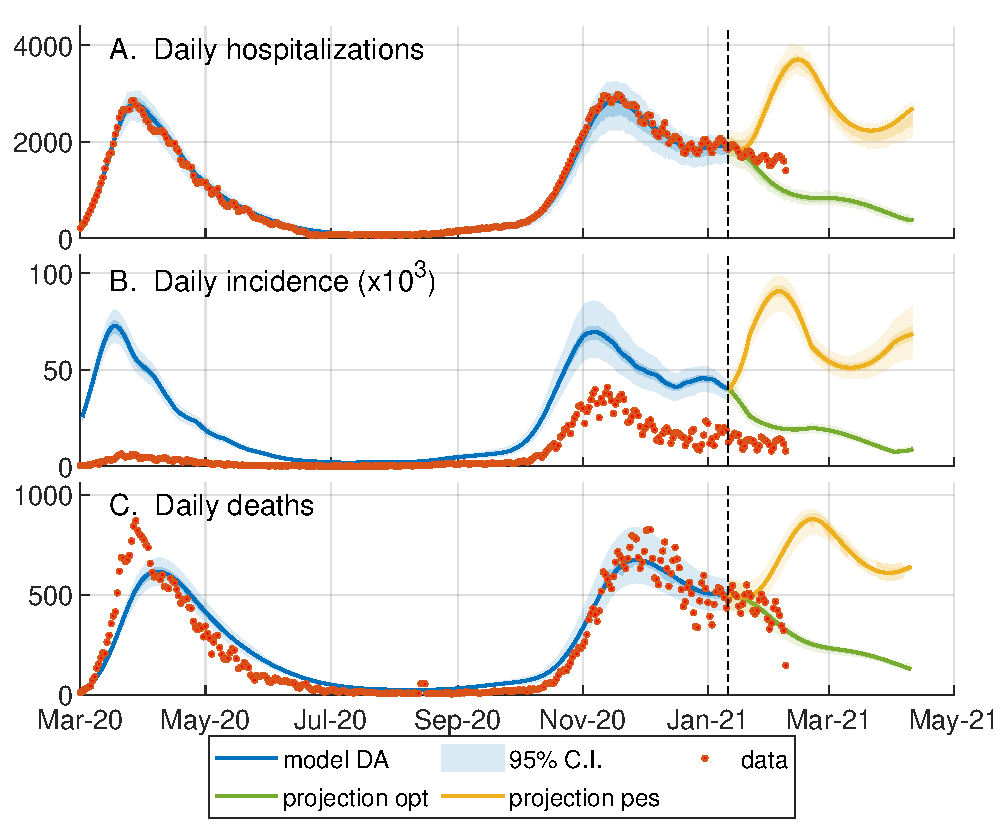
\includegraphics{fig_italy-ocp/figures/DA_italy1.pdf}
    \caption[Data assimilation and scenarios for optimization]{Data assimilation and scenarios for optimization. Comparison between the model outputs (95\% confidence interval (CI) of the ensemble, blue shaded area) and the corresponding epidemiological data from March 2020 to January 2021. The orange and green shaded area respectively show the ensemble dynamics (95\% CI) of what is called pessimistic and optimistic transmission scenarios from January to April. The optimal vaccination strategy in the optimistic (or pessimistic) scenario is computed with respect to the the continuous green (or orange) line, representing the model trajectory obtained using the median of each ensemble parameter. A. The data on the daily hospitalizations is estimated as described in \parencite{Bertuzzo:GeographyCOVID19Spread:2020}; this data at the regional level is assimilated on a moving window of 14 days to update the model parameters describing the local transmission rates (see SI). B. Daily number of newly exposed individuals versus the reported positive cases. Note that, the model assumes the presence of 90\% asymptomatics among the exposed individuals, who are possibly not detected by the surveillance system. C. Daily number of deaths. %\textbf{D.} Estimated reproduction number. The fluctuations during summer 2020 are mainly due to local outbreaks generated by  imported cases which cannot be directly considered in the model since the data is not public available.  
    }\label{fig:model_DA}
\end{figure}

\paragraph{Calibration and scenarios}The epidemiological model, previously calibrated during the first wave of COVID-19 in Italy\cite{Gatto:SpreadDynamicsCOVID19:2020,Bertuzzo:GeographyCOVID19Spread:2020}, is updated up to January 11, 2021 using an iterative particle filtering. This data assimilation scheme allows us to capture the second wave of infections that hit Italy in the Fall of 2020, a necessary requirement to generate model projections that take into account the whole epidemic history, as shown in fig.~\ref{fig:model_DA}. In our approach, model projections are described by an ensemble of a thousand trajectories associated with different parameters, whose distributions quantify the model uncertainty. 
\marginnote{The detailled methods for the data assimilation scheme is provided in the supplemental information of \parencites{Lemaitre:OptimizingSpatiotemporalAllocation:2021}, and this thesis focuses on the optimal control problem. However, data assimilation is a key compomentent allowing to update models states and parameters as new data becomes available, making it necessary of model predicitive control (see \textsc{Discussion and Conclusion}.}
Two projection scenarios are considered, each characterized by a possible rate of epidemic transmission, see fig.~\ref{fig:model_DA}. The "Optimistic" scenario assumes a constant lowering of transmission from January 11, 2021 to April 11, 2021; the "Pessimistic" scenario considers a gradual increase in transmission until mid February 2021, which results in a third wave. 

For each scenario, the optimal control problem is solved for one reference model trajectory, whose parameters and state on January 11, 2021 are obtained as the median values of the 1'000 model realizations. In this way, the reference trajectory approximately represents the ensemble median in each province. Then, the effectiveness of the optimal allocation is assessed on the full ensemble of trajectories.


%Note that, since this spatial model does not consider risk-classes, the vaccination strategy minimizing the incidence also minimizes deaths or hospitalizations.

This division is necessary in order to solve the optimal control problem (OCP) in a reasonable time. To adapt our framework to another model/country, one would need to update the "true" model to a suitable candidate (which could be a stochastic model, a Hidden Markov model, or any other kind) and design a tractable approximation of this new model to be solved by optimal control.

In order to evaluate the effectiveness of our approach, the optimal vaccination course that minimizes the objective is computed based on the simplified model. Then, this strategy and the alternative ones are evaluated on the full model, for different posterior realisations. If the simplified model is sufficiently accurate, the performance loss is small and the proposed strategy outperforms simpler strategies, as shown in our simulation results.

\subsection{Formulation of the optimal control problem}
\paragraph{Optimal control problem definition}Let $n$ the number of spatial nodes ($n=107$ provinces in Italy) and $m$ the number of epidemic states in our model ($m=9$ states).
The states of the system are noted $x(t) \in \mathbb{R}_+^{n\times m}$, i.e., $x(t)$ is a vector containing the epidemic variables $S_i(t)$, $E_i(t)$, $P_i(t)$, $I_i(t)$, $A_i(t)$, $Q_i(t)$, $H_i(t)$, $R_i(t)$, $V_i(t)$ for every province $i=1,...,n$. The rate of vaccine rollout for every node $i$ at time $t$ is written $v(t) = (v_1(t),...,v_n(t)) \in \mathbb{R}_+^{n}$, representing our control variable:. %Omitting the time dependence $t$, t

The dynamics of the epidemiological model (eqn.~\eqref{eq:sepiar}) are expressed as an ordinary differential equation in each province $i$:
\begin{equation}
    \label{eq:sepiar_compact}
    \dot x_i(t) = F_i(x_i(t),v_i(t), m_i(t), t),
\end{equation}
where $m_i(t)$ carries the contribution of other provinces to the force of infection of node $i$. The epidemiological model can be described by the following system of ordinary differential equations coupling disease transmission among all provinces:

\begin{align}
    \dot x(t) = F(x(t),v(t),m(t),t)
    \label{eq:dynamics}
\end{align}

For simplicity, the time dependence is dopped in the equations below, and the state and control variables for the full system as
\begin{align*}
    x = (x_1,\ldots,x_n), && v = (v_1,\ldots,v_n),
\end{align*}
The global dynamics for all provinces are denoted:
\begin{equation*}
    F(x,v) = (F_1(x_1,v_1, m_1),\ldots,F_n(x_n,v_n, m_n)).
\end{equation*}
The coupled force of infection in node $i$ is denoted $\lambda_i$. The cost function is defined as the national incidence, i.e., the sum of new infections (transitions $S_i\longrightarrow E_i$) in all provinces at time $t$,  for every node $i$, i.e.,

\begin{equation*}
    L(x,v) = \sum_{i=1}^n \lambda_i S_i.
\end{equation*}

For the sake of generality the terminal cost $M$ is introduced, which can be used to ensure that the system is left in a proper state instead of optimizing for short-term gain. Since properly designing the terminal cost could require a long analysis, for simplicity it is not used in this work, hence $M(\cdot) = 0$.

Given our dynamical system with states $x$, controls $v$, and dynamics $F$, the OCP is:

\begin{subequations}
    \label{eq:ocp}
    \begin{align}
        \min_{v(\cdot)} \ \ & \int_{0}^{T} L(x(t),v(t)) \ \mathrm{d}t + M(x(T)) \\ \label{eq:ocp_dyn1}
        \mathrm{s.t.} \ \ & x(0) = \hat x_0, \\ \label{eq:ocp_dyn2}
        &\dot x(t) = F(x(t),v(t)), && \forall \, t\in[0,T], \\ 
        &H(x(t),v(t)) \leq 0, && \forall \, t\in[0,T],
    \end{align}
\end{subequations}

where the aim is to minimize the cost function over the control horizon $T$, while enforcing the modeled SARS-CoV-2 transmission dynamics (eqns. \eqref{eq:ocp_dyn1} and \eqref{eq:ocp_dyn2}). Moreover, the constraints imposed by vaccine availability and the maximum vaccination rate are lumped in function $H$ that expands to
\begin{subequations}
    \begin{align}
        v_i(t) &\geq 0, && i\in\mathbb{I}_1^n, \label{eq:constr_vacc_met} \\
        \int_{t_\mathrm{d}}^{t_\mathrm{d}+1} v_i(t) \ \mathrm{d}t &\leq v_i^\mathrm{max} \propto N_i, && i\in\mathbb{I}_1^n,\ t_\mathrm{d} \in \mathbb{I}_0^T,  \label{eq:constr_day_met} \\
        \int_{0}^{t} \sum_{i=1}^n v_i(t) \ \mathrm{d}t &\leq D(t), && \forall \, t\in[0,T], \label{eq:constr_week_met}
    \end{align}
\end{subequations}

where time is measured in days, and $\mathbb{I}_a^b$ is the set of all integers $a\leq k\leq b$. eqn.~\eqref{eq:constr_vacc_met} enforces that one can only distribute a non-negative amount of vaccine doses. eqn.~\eqref{eq:constr_day_met} states the logistic constraints, which limit to $v_i^\mathrm{max}$ the amount of individuals that can be vaccinated each day in each node; here $t_\mathrm{d}$ is the time at which each day starts. The daily vaccination capacity of each province is set to be proportional to its population size $N_i$, assuming a fair distribution of the sanitary infrastructure among provinces, as shown in SI (fig.~\ref{fig:OC_logistic_constraints}). The constraint on the national stockpile is materialized by eqn~\eqref{eq:constr_week_met}, which ensures that the total vaccine allocation across all nodes does not exceed the stockpile $D(t)$. The stockpile is replenished every Monday by the delivery of new vaccines, hence $D(t)$ is a staircase function.



\paragraph{Transforming the optimal control problem into a non-linear programming problem}

\marginnote[1\baselineskip]{For an overview of the possible solution approaches for optimal control problems the interested reader is refered to \textcite{Betts:PracticalMethodsOptimal:2010,Biegler:NonlinearProgramming:2010}. In particular, in this work, a variant of direct multiple shooting \textcite{Bock:MultipleShootingAlgorithm:1984} tailored to distributed systems \textcite{Savorgnan:MultipleShootingDistributed:2011} is used.} 

The optimal control problem in eqn.~\eqref{eq:ocp} is solved by a direct method, also called \emph{first discretize, then optimize}, which transforms the control problem into a nonlinear programming problem. Within direct methods, direct multiple shooting is employed. 


Our time window $[0,T]$ is divided into a uniform time grid $t_0,\ldots,t_N$, with $N+1$ points and $t_0=0$, $t_N=T$. Hence there are $N$ intervals $[t_k,t_{k+1}]$, and the states at time $t_k$ is denoted $x_k=x(t_k)$, and $v_k$  represent the controls in interval $[t_k,t_{k+1}]$. The control function is parameterized using basis functions with local support. \marginnote[-2.5\baselineskip]{For discretization, a uniform time grid is choosen here, i.e., $t_{k+1}=t_k+\delta_t$ and a piecewise constant control function, i.e., $v(t)=v_k$, $t\in [t_k,t_{k+1}]$. This is a common choice but other are possible. Here $\delta t=1\ \mathrm{day}$.}

The continuous-time dynamics~$F$ in eqn.~\eqref{eq:dynamics} are transformed by numerical integration into the discrete-time operator $f$ by numerical integration. The system dynamics are then discretized to obtain a discrete-time system.

\begin{align*}
    x_{k+1} = f(x_k,v_k),
\end{align*}

satisfying $x_k=x(t_k)$ for all $k=0,\ldots,N$. Moreover, the cost function is also discretized, to obtain

\begin{align*}
    l(x_k,v_k)=\int_{t_k}^{t_k+1} L(x(t),v(t)).
\end{align*}

The discretization is performed using numerical integration techniques (such as a fourth-order Runge-Kutta scheme, with 50 steps per days) to obtain a good approximation of the true trajectory and cost. Finally, the path constraints $H$ are relaxed and imposed at a finite amount of time instants, here coinciding with the time grid $t_0,\ldots,t_N$. Since in our case the constraints only involve the controls, no approximation is introduced by enforcing these constraints only on this uniform grid. The OCP~\eqref{eq:ocp} is then approximated by the nonlinear programming problem

\begin{subequations}
    \begin{align}
        \min_{x,v} \ \ & M(x_N)+\sum_{k=0}^{N-1} l(x_k,v_k)  \\ 
        \mathrm{s.t.} \ \ & x_0 = \hat x_0 \\
        & x_{k+1} = f(x_k,v_k), && k\in \mathbb{I}_0^{N-1}, \\
        &H(x_k,v_k)\leq 0, && k\in \mathbb{I}_0^{N-1}.
    \end{align}
        \label{eq:ocp_nlp}
\end{subequations}
\marginnote[-7\baselineskip]{%In~\eqref{eq:ocp_nlp}, 
Here both the states $x=(x_0,\ldots,x_N)$ and the controls $v=(v_0,\ldots,v_{N-1})$ are defined as optimization variables, which is a distinguishing trait of multiple shooting as opposed to single shooting.}

The force of infection associated with mobility is assumed to constant over each day. Thus, each node dynamics can be made independent of the other nodes dynamics by introducing an auxiliary control variable $z$ that is constrained to match the force of infection due to the other nodes at the beginning of each time interval. Then, the dynamics of the decoupled system in each node can be written as:

\begin{align*}
\dot x_i(t) &= F_i(x_i(t),z_{i,k}), && t\in[t_k,t_{k+1}] \\
x_i(t_k) &= x_{i,k} + g_i(v_{i,k}), && z_{i,k} = e_i(x).
\end{align*}

\paragraph{Solving the Non-linear programming problem} Nonlinear programming problems may be solved by readily available solvers using the primal-dual interior point method. The main difficulty in solving the proposed nonlinear programming problem \eqref{eq:ocp_nlp} is the large dimension of the system and the non-linearities of the model. In order to bring the problem to a tractable form, three simplifications are introduced: (a) vaccines are administered instantaneously at the beginning of each day, rather than with a constant rate over the whole day; (b) the component of the force of infection taking into consideration the mobility of individuals across provinces is evaluated at the beginning of each day and remains constant through the day; and, (c) the mobility network is simplified, by keeping only the most important connections (see fig.~\ref{fig:model_description_network}), thus increasing the sparsity of the underlying spatial connectivity matrix. These simplifications deliver a significant computational advantage, and the impact on the model  accuracy was verified to be limited. 
\marginnote[-11\baselineskip]{Note that, even if the optimal strategy is computed using the simplified model, its impact in terms of averted cases and deaths is evaluated using the full epidemiological model without any of these simplifications. A more detailed discussion on this subject, and on the impact of the simplification is given in the \textsc{Appendix to Chapter 7}.}
\marginnote[-2\baselineskip]{The full framework and analysis code is available here: \url{https://github.com/jcblemai/COVID-19_italy-vaccination-oc}.} 
The nonlinear programming problem arising from the simplified epidemiological model is non-convex, and involves approximately $10^{5}$ variables and $10^5$ constraints. The problem is formulated within the automatic differentiation framework CasADi\cite{Andersson:CasADiSoftwareFramework:2018} and solve it using Ipopt~\cite{Wachter:ImplementationInteriorpointFilter:2006} with the HSL ma86 large sparse symmetric indefinite solver\cite{HSLCollectionFortran}, which exploit the sparsitity of the problem. 
Solving the OCP is both CPU and RAM intensive. Numerical computations are preformed on the Helvetios cluster the EPFL HPC facility (one problem per computing node, each equipped with 36 2.3 GHz cores and 192 GB RAM). On this cluster, it takes approximately four days to solve the large-scale OCP just presented. It should be possible to solve even larger problems with more RAM available. 


%% ***********************************************************************************************
\section{Results}
%% ***********************************************************************************************
Using state-of-the-art linear algebra solvers and automatic differentiation, each scenario (optimistic and pessimistic, with different weekly stockpile deliveries) is solved for the optimal vaccination allocation. The optimal vaccination strategies are obtained for a set of eight scenarios drawn from the spatial model from January 11, 2021 to April 11, 2021. These scenarios are a combination of two projection scenarios (pessimistic vs optimistic) and four assumptions on the weekly stockpile delivery (479'700, 1M, 1.5M or 2M doses delivered per week). In each scenario, the optimal solution is a spatially explicit vaccine roll-out policy, i.e. an indication of the number of vaccine doses to be deployed in each province each day. 
%% ***********************************************************************************************
\subsection*{Comparison of vaccination strategies}
In order to measure the potential impact of the optimal allocation strategy, it is compared against three non-optimized, yet reasonable alternative approaches: vaccinate proportionally to the future incidence as projected by the epidemiological model; vaccinate proportionally to the number of susceptible individuals in each province; vaccinate proportionally to the province's population. 
Comparisons with additional alternative strategies are presented in SI. Spatial prioritization based on epidemiological criteria, such as past\cite{Lee:AchievingCoordinatedNational:2020} or future\cite{Pasetto:RealtimeForecastingCholera:2018} incidence, has been thoroughly used in real campaigns and prospective studies.

For each of the eight scenarios considered, the number of averted infections is computed with respect to a zero-vaccination baseline, and the number of averted infections per vaccination dose (see tab.~\ref{table:averted_abs}). In the optimistic transmission scenario, characterized by a recess of the epidemic, the vaccination campaign has a lower impact on the averted infections per dose as only a small percentage of the vaccinated individuals would have been at risk of transmission. Obviously, the impact of the vaccination campaign is more evident in the pessimistic scenario where, for all strategies, the averted infections are larger than the vaccines deployed due to indirect protection effects. By virtue of the law of diminishing returns, the number of averted infections per dose decreases when increasing the stockpile. 

\begin{table*}[h!]
\centering
\begin{tabular}{clrrrr}
\toprule
Weekly stockpile& {} & \multicolumn{2}{c}{Averted Infections} & \multicolumn{2}{c}{Averted Infections} \\
delivery&  {}  &\multicolumn{2}{c}{(Millions)} & \multicolumn{2}{c}{ per doses} \\
& Method &  Optimistic & Pessimistic &     Optimistic & Pessimistic \\
\midrule
2 millions & \textsc{Optimal} &   $6.98$ &  $30.6M$ & $0.268$ & $1.18$ \\
        & Incidence &   6.32 &    28.1 &          0.243 &        1.08 \\
        & Population &   6.02 &    26.8 &          0.231 &        1.03 \\
        & Susceptibility &   5.97 &    26.7 &          0.229 &        1.02 \\
1.5 millions & \textsc{Optimal} &   $5.52$ &   $24.1$ &  $ 0.283$ & $1.24$ \\
        & Incidence &   4.89 &    21.7 &           0.25 &        1.11 \\
        & Population &   4.57 &    20.4 &          0.234 &        1.05 \\
        & Susceptibility &   4.51 &    20.3 &          0.231 &        1.04 \\
1 million & \textsc{Optimal} &    $3.9$ &    $16.9$ &  $0.3$ & $1.3$ \\
        & Incidence &   3.41 &    15.1 &          0.262 &        1.16 \\
        & Population &   3.08 &    13.8 &          0.237 &        1.06 \\
        & Susceptibility &   3.02 &    13.7 &          0.232 &        1.05 \\
479'700 & \textsc{Optimal} &  $2.01$ &  $8.54$ & $0.322$ & $1.37$ \\
        & Incidence &   1.73 &    7.57 &          0.278 &        1.21 \\
        & Population &   1.49 &    6.74 &          0.239 &        1.08 \\
        & Susceptibility &   1.43 &    6.54 &          0.229 &        1.05 \\
\bottomrule
\end{tabular}

\caption[Averted infections per dose for different allocation strategies]{Absolute number of averted infections and averted infections per dose during the first three months of 2021 as evaluated for the reference trajectory (see fig.~\ref{fig:model_DA}, and fig.~\ref{fig:OC_comparison} for an assessment on a set of trajectories drawn for the posterior distribution). The first column represents the considered scenarios of weekly stockpile replenishment, i.e.~the number of doses delivered to Italy every week, ranging from 479'700 to 2M.}
\label{table:averted_abs}
\end{table*}
\begin{figure}[!ht]
    \centering
    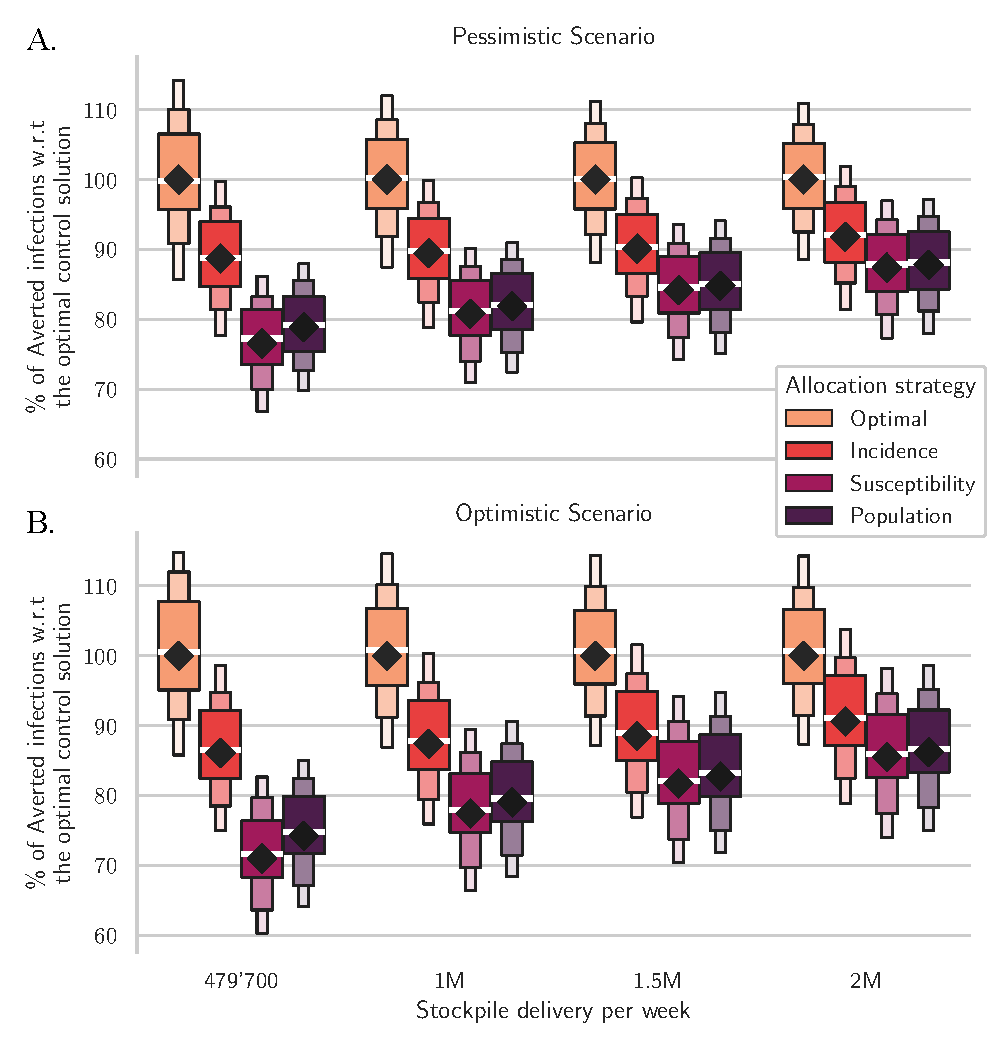
\includegraphics[width=\textwidth]{fig_italy-ocp/figures/scenarios_perturb_all.pdf}
    \caption[Comparison between different vaccine allocation strategies]{Comparison between different vaccine allocation strategies. Percentage of averted infections per vaccine doses from January 11, 2021 to April 11, 2021 resulting from province-scale vaccine allocation strategies for both the pessimistic (panel A) and the optimistic (panel B) scenarios based on: the optimal solution, population, proportion of susceptible individuals, and projected incidence (see color codes in the legend). The vaccine allocation is optimized for a (median) reference trajectory (diamonds), and assess the performance of the computed vaccination strategy over the whole posterior (box plots). For each projection scenario, results are normalized by the number of averted infections in the reference solution (see tab.~\ref{table:averted_abs} for absolute values). Results for alternative scenarios and vaccination strategies are shown in fig.~\ref{fig:OC_comparison_all}.}
    \label{fig:OC_comparison}
\end{figure}
The optimal solution always outperforms all alternative strategies in terms of the number of averted infections and in terms of averted infections per dose (see again tab.~\ref{table:all_strat}). Incidence-based allocation comes second, while population and susceptibility-based allocation are distant third and fourth respectively. The improvement between optimal and incidence-based allocation is significant, ranging from 8.8\% (pessimistic, 2M doses/week) to 16.2\% (optimistic, 479'000 doses/week). In fig.~\ref{fig:OC_comparison}, the black diamonds represent the percentage of adverted infections obtained using each strategy for the reference trajectory, with respect to the averted infections resulting from the optimal strategy. The optimal strategy is observed to have the largest relative benefits for the smallest stockpile in both the optimistic and pessimistic scenarios. 

In the pessimistic scenario (see fig.~\ref{fig:OC_comparison}.A), when 479'700 doses are made available each week, the averted infections associated with the optimal strategy in the reference projection are 1.37 per dose: $25~\%$ more compared to the strategies based on population or susceptible distributions (1.08 averted infections per dose), and more than $10~\%$ higher compared to the strategy based on the projected infections (1.21 averted infections per dose). These differences are smaller but still significant when increasing the weekly stockpile deliveries up to 2M doses; similar results are obtained also for the optimistic transmission scenario (fig.~\ref{fig:OC_comparison}.B). 

The optimal control strategy considered here is computed for a reference model trajectory, which is the median of an ensemble of 1000 realizations. To further investigate the effectiveness of the optimal solution, it is applied to a subset of trajectories randomly sampled from the ensemble. The box plots in fig.~\ref{fig:OC_comparison} display the main quantiles of the averted infections computed for the ensemble of trajectories. The optimal strategy still yields better results than the ensemble of projections related to the other strategies, thus suggesting that the computed solution is robust even under the presence of perturbations in the forecasts of the epidemic dynamics. More importantly, for each realization of the ensemble and for each projection scenario, the optimal strategy systematically averts more infections than any of the other control strategies.

Our results suggest that it is possible to considerably increase the impact of vaccination campaigns by optimizing the vaccine allocation in space and time. For this task, optimal control provides the best possible strategy and sets a benchmark for the theoretical potential of a vaccination campaign.

%% ***********************************************************************************************
\subsection*{Analysis of the optimal vaccine allocation}

\begin{figure}[!ht]
    \centering
    %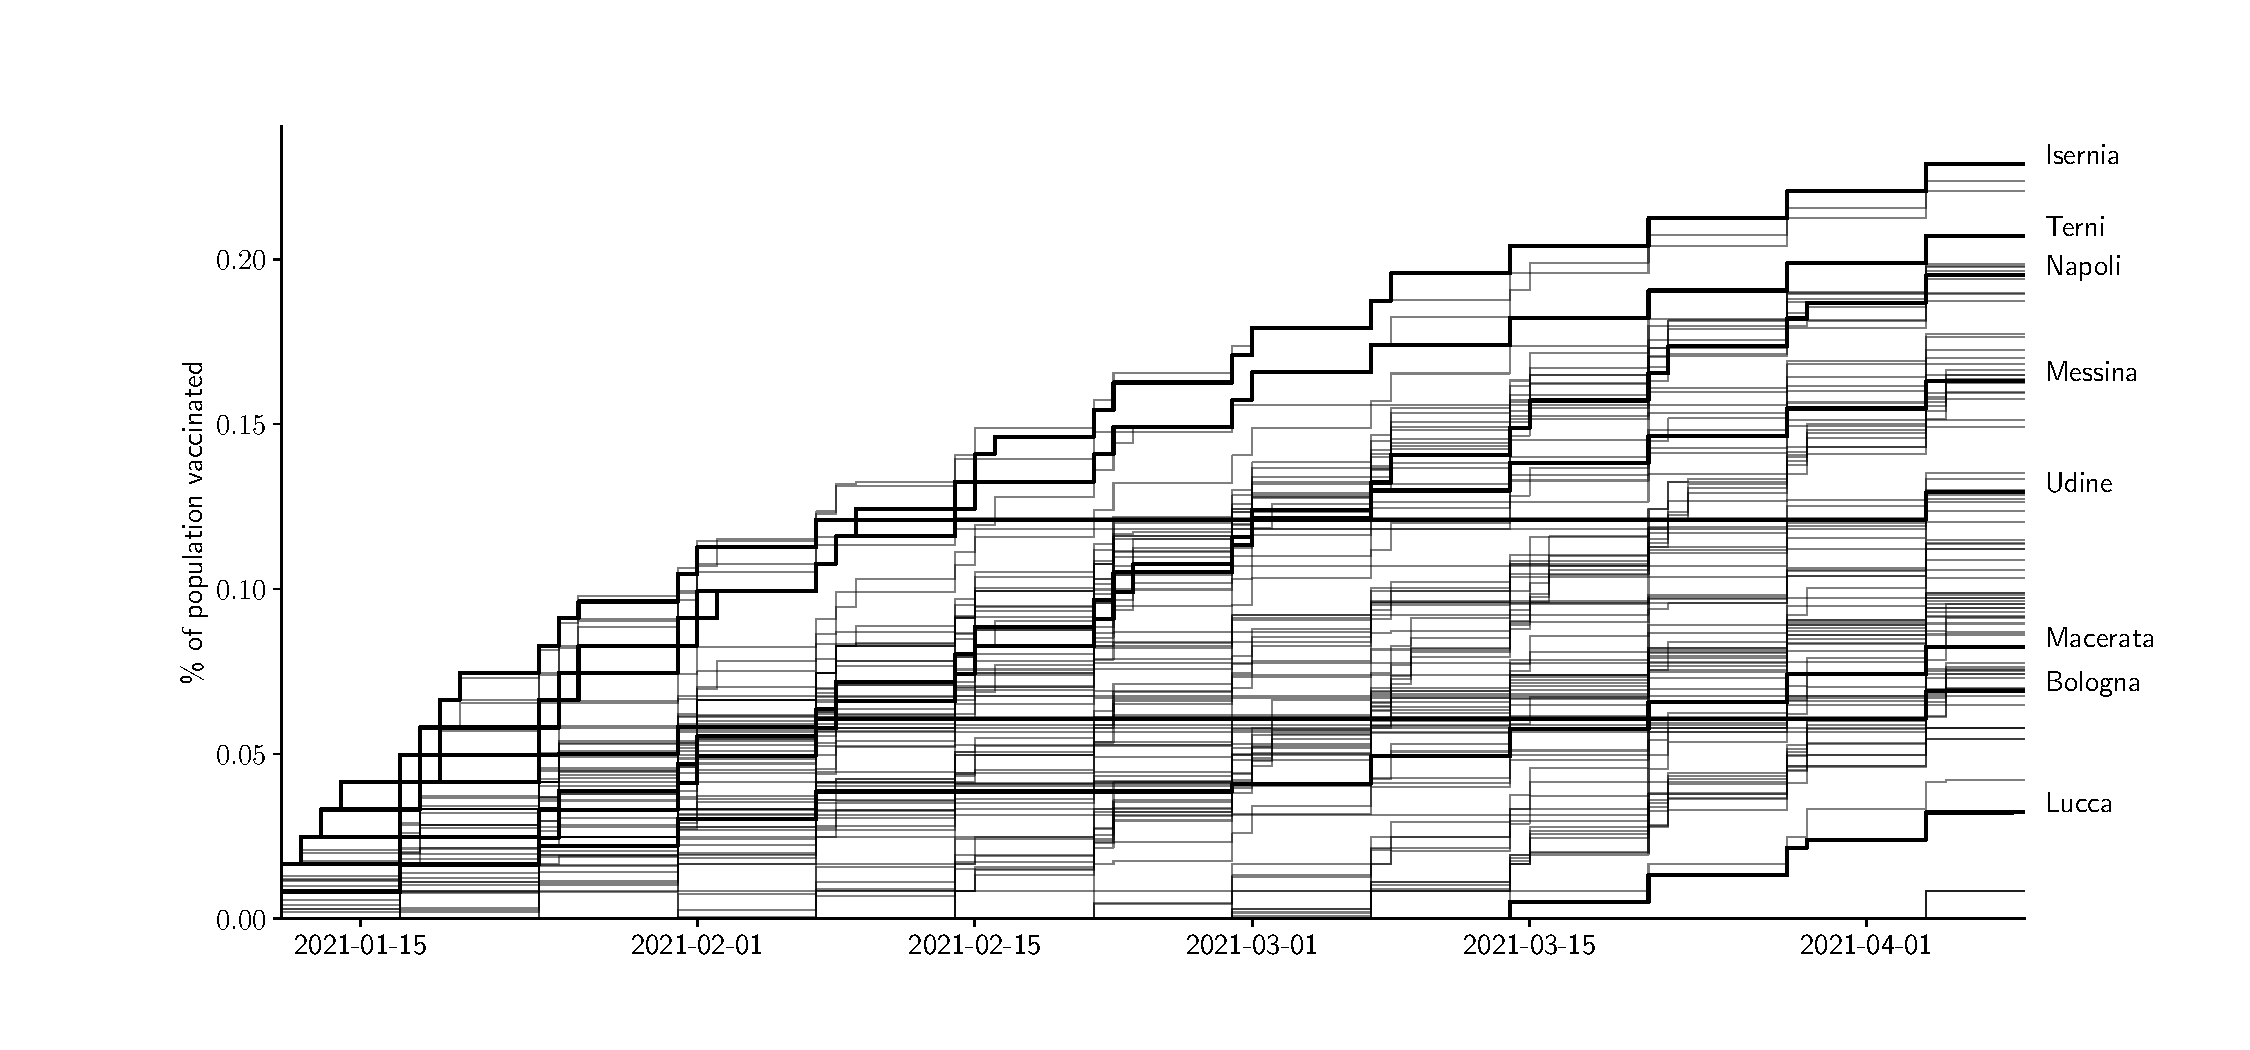
\includegraphics[scale=0.23]{figures/ts_optimal_selected.pdf} \\
    %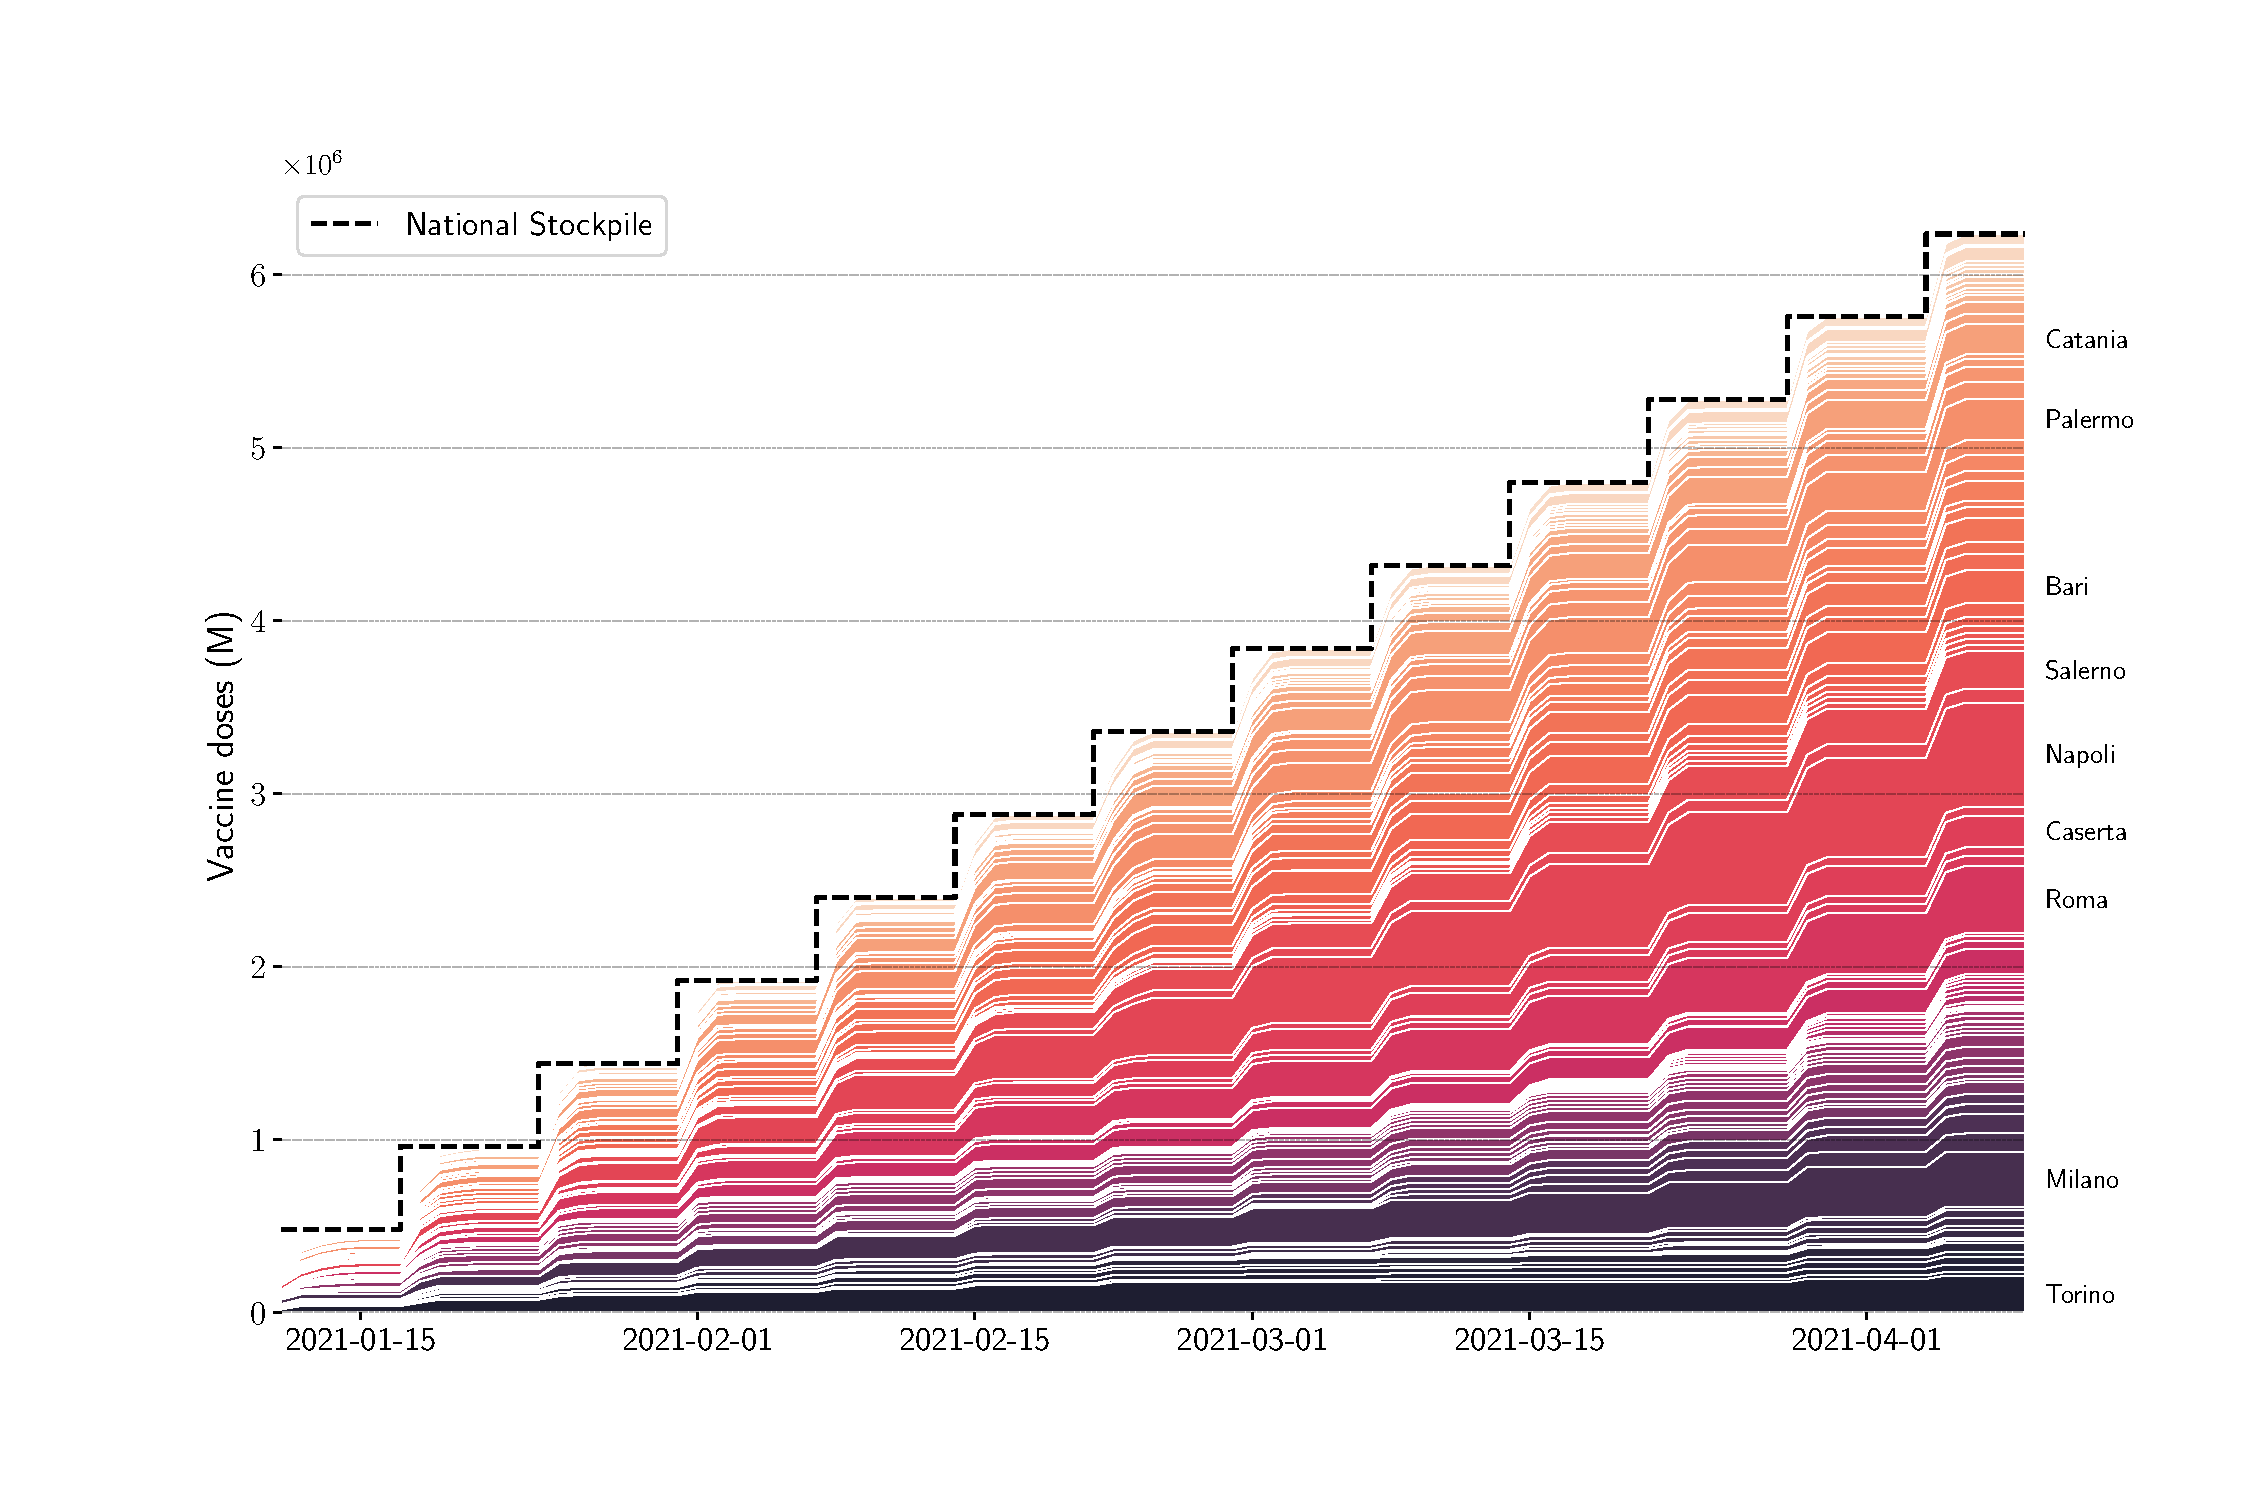
\includegraphics[scale=0.23]{figures/ts_optimal_stackplot.pdf}
    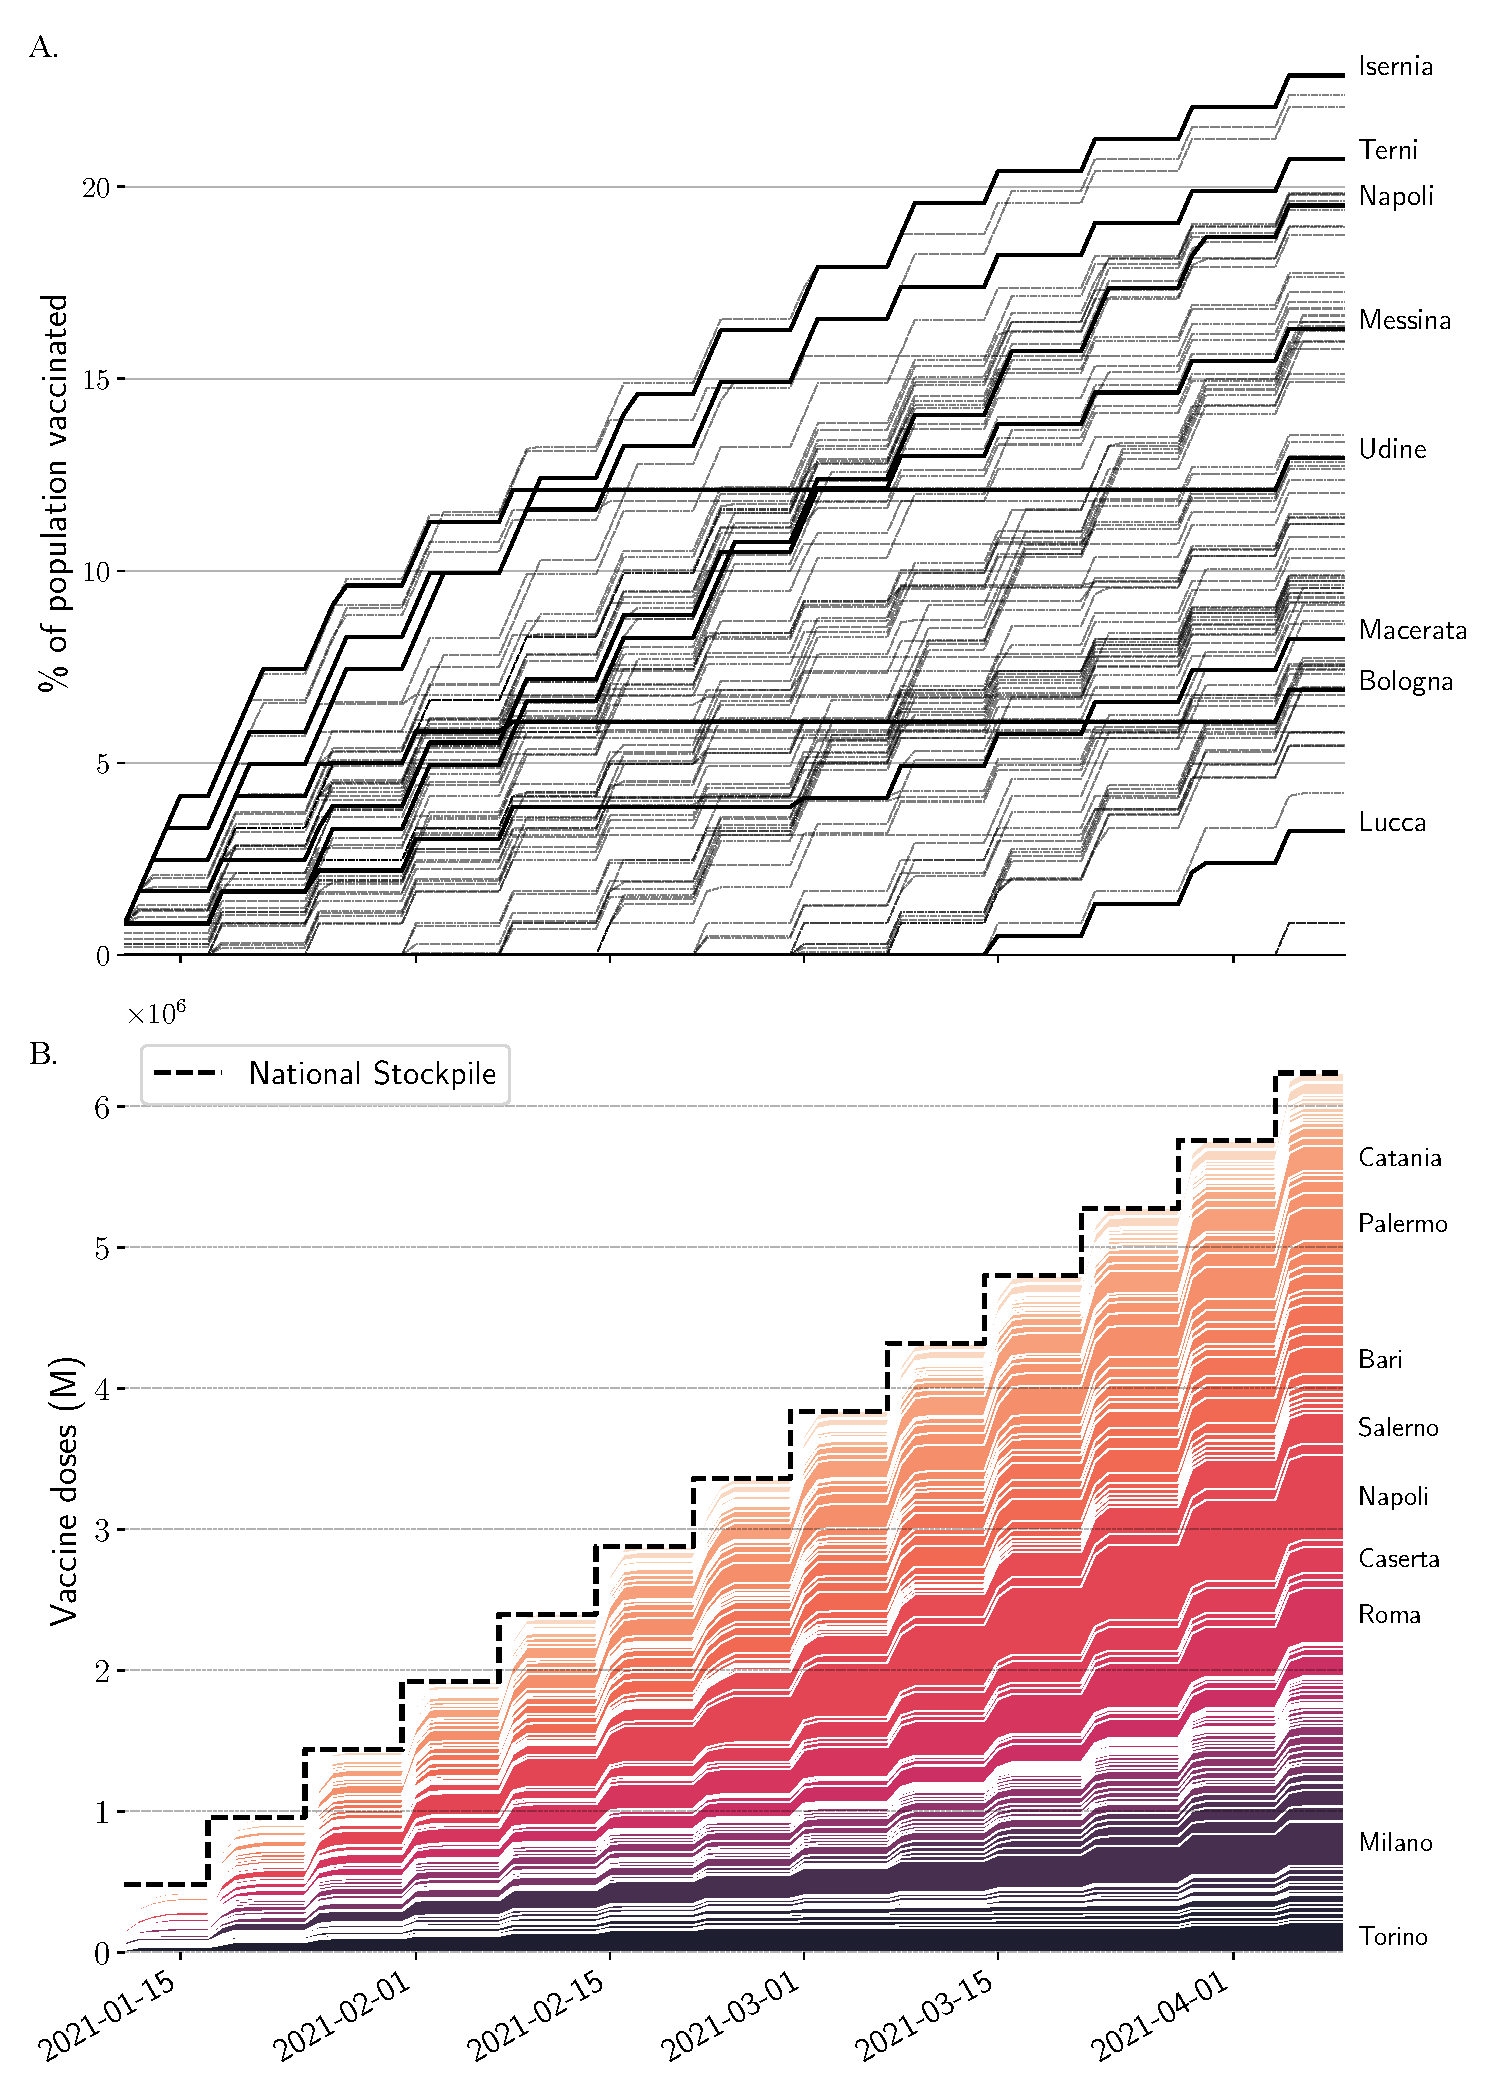
\includegraphics[width=\textwidth]{fig_italy-ocp/figures/ts_both.pdf}
    \caption[Optimal vaccine allocation for the baseline, pessimistic scenario. ]{Optimal vaccine allocation for the baseline, pessimistic scenario. \textsc{A.} Cumulative proportion of vaccine doses administered in the 107 provinces, (some of which are highlighted) . The local distribution rate is limited by a rate that is proportional to population. This logistic constraint is visualized here as the maximum slope, equal for every province.
    \textsc{B.} Stacked cumulative absolute number of vaccines in the 107 provinces of Italy. The national stockpile is shown in black, and is replenished every week (say on Mondays) with 479'700 doses. The name of the provinces with a final allocation of more than 150'000 doses is shown on the right.}
    \label{fig:OC_stackplot}
\end{figure}

The optimal vaccine allocation obtained as the solution of the optimal control framework is complex to analyze.%, and w- ought to do that by unraveling the mechanism behind its performance.
The strategy must obey the imposed logistic and supply constraints: 1) The vaccine stockpile is replenished every Monday by a fixed amount of doses (e.g., 479'700 doses in the baseline scenario), and 2) the maximum possible distribution capacity per province is limited, proportionally to the node population, so that the number of doses distributed across the country can be of 0.5M per day at maximum (more details in SI fig.~\ref{fig:OC_logistic_constraints}). \begin{marginfigure}[-10\baselineskip]
    \centering
    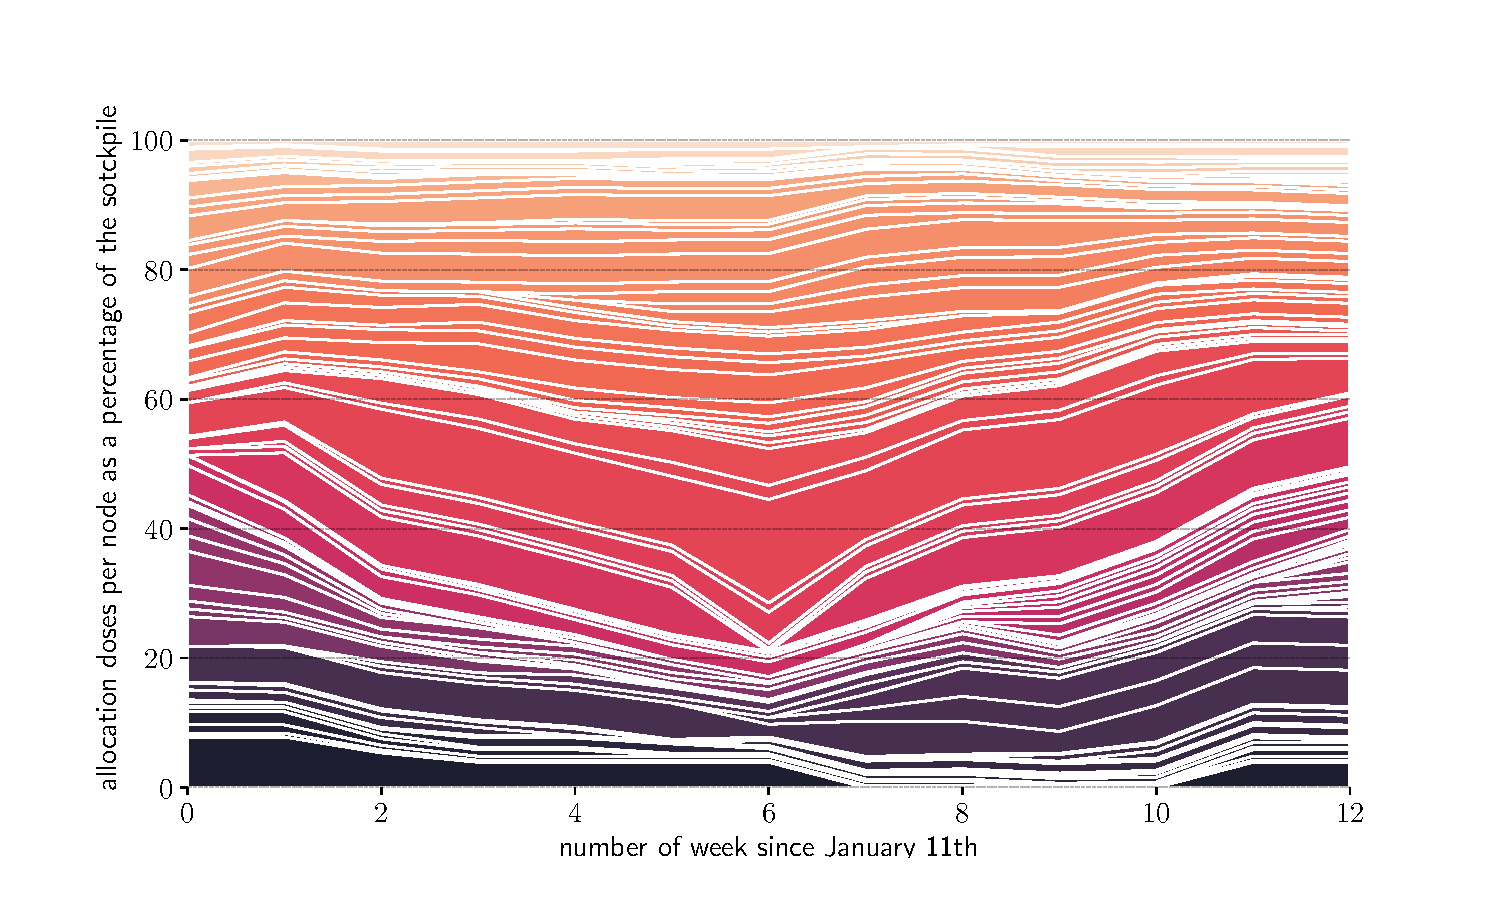
\includegraphics{fig_italy-ocp/figuresSI/SI_ts_optimal_stackplot_proportional.pdf}
    \margincaption[Time allocation for the pessimistic scenario]{Time allocation for the pessimistic scenario with a stockpile delivery of 479'700. Each week, the 479'700 doses are spread accross the provinces. This view unravel the temporal pattern in the allocation.}
    \label{fig:OC_temporal_alloaction}
\end{marginfigure}

The optimal vaccination course in time for the pessimistic, 479'700 doses/week scenario is shown in fig.~\ref{fig:OC_stackplot}. The optimal allocation respects is observed the two constraints on distribution (fig.~\ref{fig:OC_stackplot}, A) and supply (fig.~\ref{fig:OC_stackplot}, B). Moreover no province is vaccinated at the maximum possible rate during the whole campaign, and that provinces display a variety of vaccination patterns. Last, note that the vaccines received every Monday are always distributed during the following week, but that the rate of delivery on a national level increases with time (fig.~\ref{fig:OC_stackplot}, B). Surprisingly, the optimal solution favors precise targeting over speed of delivery, in order to allocate more doses to those provinces where the impact of vaccines on the whole system is projected to be higher. Hence, in order to control infections, precise targeting may trump delivery speed. 

\begin{figure*}[!ht]
    \centering
    \includegraphics[width=1.1\textwidth]{fig_italy-ocp/figures/map_all.pdf}
    \caption[Spatial vaccine distribution patterns]{Spatial vaccine distribution patterns for the optimal allocation (left) and alternative strategies based on population, incidence and susceptibility (additional alternative strategies are presented in the \textsc{Appendix}). For each province and strategy is shown: the proportion of vaccinated individuals (top), the number of averted infections per inhabitant with respect to a no vaccination baseline (middle), and the proportion of individuals who are still susceptible at the end of the control horizon (bottom). Visual inspection suffices to reveal that the optimal allocation strategy is more alike the incidence-based allocation, but with vaccine doses spread-out to more provinces.}
    \label{fig:OC_multimap}
\end{figure*}

Furthermore, in the optimal solution every time a province is vaccinated, the rate of vaccination is equal to the maximum rate allowed by the local logistic constraint. This property is common to the alternative vaccination strategies, hence the difference in performance is due to the spatial allocation patterns.% of the optimal strategies provide the edge over the other strategies. 
In fig.~\ref{fig:OC_multimap}, one can already see by visual inspection that the optimal allocation distributes most of the available doses on a few provinces with high incidence. These provinces are neither the most connected nor the most populous in Italy. The optimal strategy makes then use of the information on the network connectivity to fine-tune the allocation, and deploys the vaccination on more provinces than the incidence-based strategy. %These little optimizations add up to the significant improvement seen above.

To further investigate these patterns, in fig.~\ref{fig:OC_scatter}.A is shown the number of administered doses vs the incidence projected without vaccines (the proxy variables leading to the second-best control performance), both normalized according to the resident population in each province. Sn allocation pattern whereby provinces with a higher incidence receive more vaccines is observed. However, the allocation is non-linear with respect to the projected incidence, suggesting that to better control the epidemic, the optimal allocation strategy takes into account other factors such as the importance of each province within the mobility network, as well as the proportion of susceptibles. When the weekly stockpile delivery is increased, as shown in fig.~\ref{fig:OC_scatter}.B, this pattern shifts to the right while remaining qualitatively consistent. Hence, the optimal allocation strategy is robust with respect to the overall vaccine availability constraint, and the same nodes are prioritized. Scatter plots with other covariates are shown in SI (fig.~\ref{fig:OC_scatter_optimistic}--\ref{fig:OC_scatter_optimistic}). 

\begin{figure}[!ht]
\centering
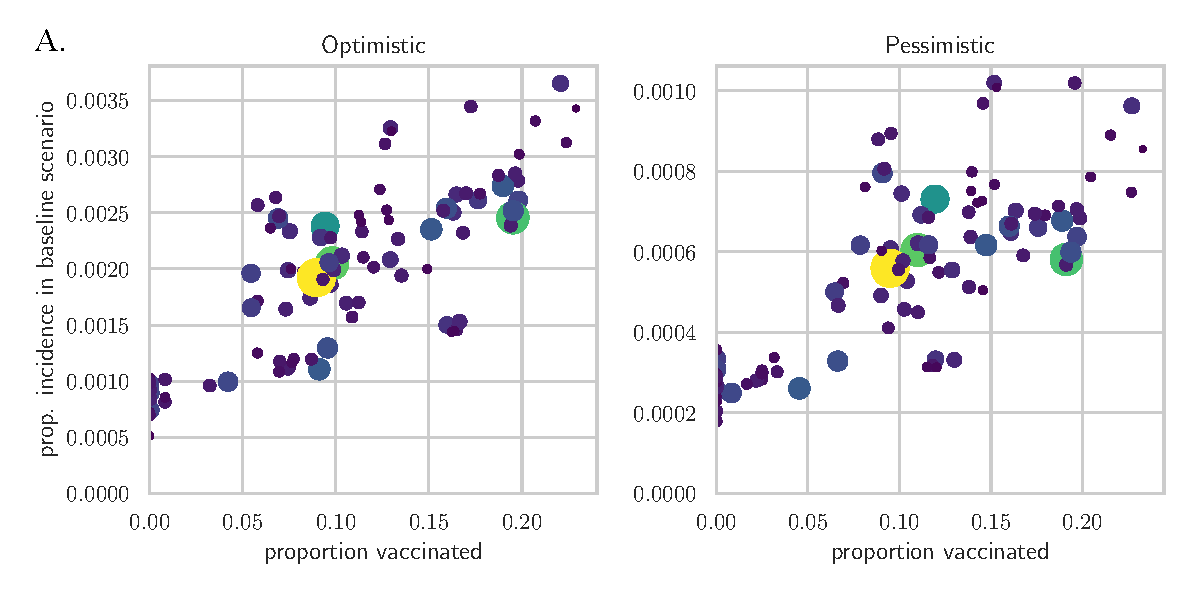
\includegraphics{fig_italy-ocp/figures/scatter_top.pdf}
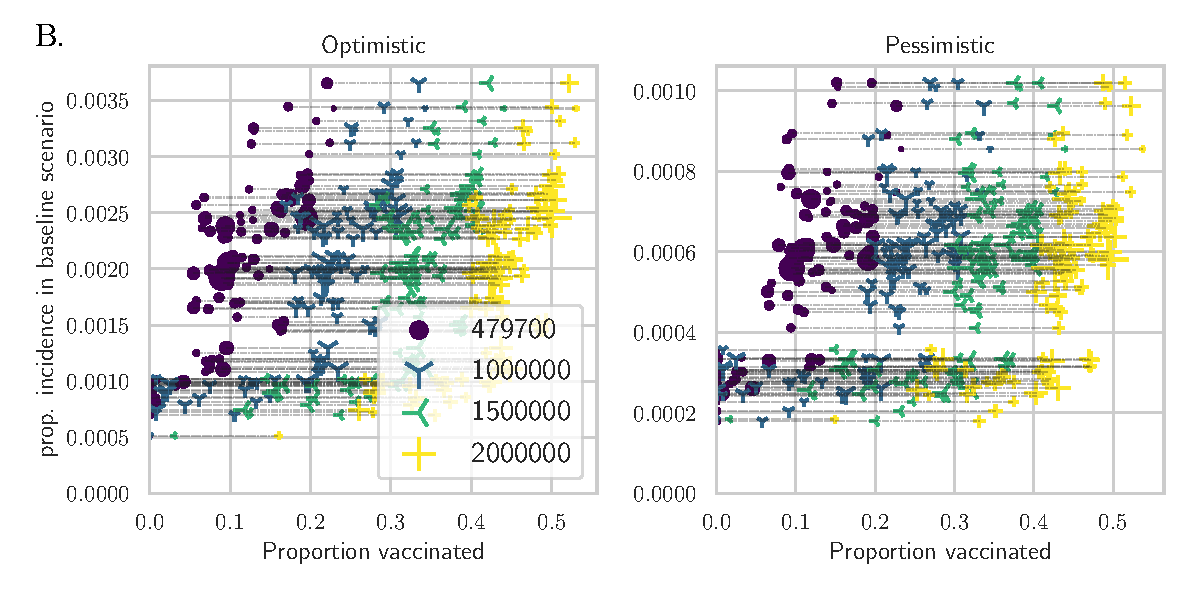
\includegraphics{fig_italy-ocp/figures/scatter_scn.pdf}
\caption[Analysis of the optimal solution]{Analysis of the optimal solution. A. Vaccinated population according to the optimal strategy against the projected incidence without vaccination, both normalized by provincial population size and considering the scenario with a weekly stockpile delivery of 479'700 doses. B. Same as in A, but considering all four scenarios of weekly stockpile replenishment. Each dot represents a province, with dot size proportional to its population.}
    \label{fig:OC_scatter}
\end{figure}


%% ***********************************************************************************************
\section{Discussion and Conclusion}
%% ***********************************************************************************************
Without any constraint on supply, each country would vaccinate its population as fast as possible according to the available infrastructure. However limitations in vaccine supply and rate of delivery are a reality for every country, hence the available doses should be deployed in space and time following a fair and effective strategy. 

In stockpile-limited settings, like most current vaccination campaigns worldwide, careful allocation may significantly increase the number of averted infections and deaths. The goal is to distribute the vaccines where they have the strongest beneficial impact on the dynamics of the epidemic. However, deriving an algorithm capable of computing spatially optimal allocation strategies in real, heterogeneous settings is far from trivial and our approach is, to the best of our knowledge, the first attempt in this direction. 

An novel optimal control framework has been developed, that delivers the best vaccination strategy under constraints on supply and logistics. This allows us to compute the allocation strategy that maximizes the number of averted infections during a projection of the COVID-19 epidemic in Italy from January 11, 2021 to April 11, 2021. Our results show that the optimal strategy has a complex structure that mainly reflects the projected incidence of each province, but also takes into account the spatial connectivity provided by the mobility network and the landscape of acquired population immunity. Although the reason why this strategy is optimal is not immediately intuitive, our simulations clearly outline its better overall performances over other, more straightforward strategies. This comparison suggests that the simplicity underlying intuitive vaccination strategies may undermine their effectiveness, and calls for complementing these simple approaches with rigorous and objective mathematical tools, like optimal control, that allow a full account of the complexity of the problem.

The present work demonstrate that it is possible to solve optimal control problems for spatially explicit dynamical models of infectious diseases at a national scale, thus overcoming the computational limitations that, up to now, precluded this kind of applications. The proposed framework can account for any compartmental epidemic model, with up to hundreds of connected spatial nodes. Supply and logistic constraints can be adapted to the actual landscape of decisions faced by the stakeholders, such as no/reduced vaccine delivery on weekends, or the need for fairness in vaccine distribution, e.g. by ensuring that each region receives at least a fixed fraction of the available vaccines. This is especially important as in our optimal allocation scenarios, some provinces receive no vaccine at all. Moreover, the optimization can be carried for single-dose vaccines, as done here, or for two-dose vaccines, where one could potentially optimize the time between the first and second dose (and if a second dose should be administered at all), clearly also considering the intervals recommended by the health authorities.

% Limitations
The method developped is obviously not devoid of limitations. The main one is that the optimal vaccination strategy strongly depends on the projection of the underlying epidemiological model. These projections are subject to several sources of uncertainty, especially for long term horizons, for example due to model design and calibration\cite{Cramer:EvaluationIndividualEnsemble:2021}, the generation of baseline transmission scenarios, and unforeseen events that may change the course of the epidemic (such as the importation of cases, the emergence of new virus variants, changes in disease awareness or social distancing policies). The optimal vaccination strategy is thus reliable only if the projections given by the underlying model dynamics are sufficiently accurate. A successful approach developed by the automatic control community to tackle that issue, named Model Predictive Control~\cite{Rawlings:ModelPredictiveControl:2017}, consists in compensating the performance losses expected over long horizons by constantly adapting the optimal strategy. In this context, Model Predictive Control might be implemented using the following steps: (a) at the beginning of each week, the state of the system is estimated by using newly acquired epidemiological data; (b) the optimization problem is solved over a fixed prediction horizon using the estimated state as initial condition; (c) the optimal strategy for the first week is applied and, as soon as the next weeks starts, these steps are repeated starting from (a). This method corrects the model inaccuracies by constantly resetting the initial state to the estimated one. Moreover, constraints may be updated to account for unexpected deliveries or new orders. Future work will aim at further evaluating the benefits of implementing this scheme for the design of optimal vaccination strategies.

Moreover, the epidemiological model underlying our control optimization has known validity and limitations\cite[-3\baselineskip]{Gatto:SpreadDynamicsCOVID19:2020, Bertuzzo:GeographyCOVID19Spread:2020}. An additional limitation of the model for the specific scopes of this work is that it does not account explicitly for risk-based classes, and thus does not account for the heterogeneities that may result from the demography of the population, as well as from the age-related transmission and clinical characteristics associated with COVID-19. While surely limiting for operational use of the tools, the scope of this \textsc{Chapter} is to provide a proof-of-concept of the relevance of spatial effects, which have not been addressed so far in the literature. To that end, our results support the relevance of the research question posed. Our framework can anyway be extended to optimize across both spatial and risk heterogeneities. 

A counter-factual assumption in this work is tha a one-dose vaccine with full and instantaneous efficacy against transmission is considered. At the time of development, the details about COVID-19 vaccines were not released, and this hypothesis allowed us to demonstrate our framework in a simple setting. Our framework can be further extended to account also for the simultaneous deployment of different vaccine types, some of which may require the administration of two doses. This extension too is subject of ongoing research, in particular to extend the modeling tools described here to accommodate the peculiarities of each authorized vaccine candidate while designing effective spatiotemporal deployment strategies.

% Conclusion
In conclusion, in this work the vaccine allocation at country scale has been optimized on different scenarios of epidemic transmission and vaccine availability. A spatially explicit compartmental model that had already been successfully used to describe the COVID-19 pandemic in Italy is updated using a data assimilation scheme. Then, the model is  discretized, transformed and simplified and a pipeline is constructed to perform large-scale nonlinear optimization on vaccine allocation, subject to stockpile and logistic constraints. Solving this problem yielded a complex solution that outperforms other strategies by a significant margin and proves robust across posterior realizations of the underlying model. As such, beside inherent limitations, it provides a benchmark against which other, possibly simpler vaccine rollout strategies can be usefully compared.

 % 6
\chapter*{Conclusion and Perspectives}
\addcontentsline{toc}{chapter}{Conclusion and Perspectives}
\markboth{Conclusion and Perspectives}{}
Each of the five chapters presented in this thesis introduce an infectious disease model tailored to tackle a public-health policy related question, whether related to infectious disease transmission pathways or to the effects of control policies. Each study take a different path within the interactive process to model infectious diseases, see \textsc{Introduction}, fig. \ref{fig:modeling}. Naturally, the angle of attack to approach the complex phenomenas that are cholera and \textsc{covid}-19 varies with the studied disease and the research question but also with many factors that set the stage for the study, among which \eg the data available, the potential collaboration with decision-makers. Let's go through this conversation of models one more time.

First, as in classical hypothesis testing, a model might be considered as a simplified representation of reality. Among different hypothesis, the aim is to find the ``true'' model underlying the observed dynamics. This perspective is taken in \textsc{Chapter~2}, where the explanatory power of different pathways for rainfall-mediated cholera transmission are compared\cite{Rinaldo:Reassessment20102011:2012, Eisenberg:ExaminingRainfallCholera:2013}. Results stress the importance of rainfall as a covariate for cholera transmission while highlighting the complexity of the mechanistic pathways considered. While context-dependent, it is nevertheless interesting to observe how different transmission routes proposed in the literature fare on intra-seasonal rainfall events in Juba, South Sudan.

Policy relates questions in \textsc{Chapters 3} and 4 change the outlook and predictive accuracy with respect to interventions and transmission of interest is desired; models that most adequately reproduce an unknown, highly complex reality in order to perform experiments are designed\footnote{Indeed, accurate mechanistic modeling is still required for the processes of interest and these two perspectives are more related than opposed}. As a part of multi-modeling study\cite{Lee:AchievingCoordinatedNational:2020}, a spatial stochastic model of cholera transmission in Haiti is proposed in \textsc{Chapter~3}. Building on ECHO's experience on cholera modeling\cite{Rinaldo:Reassessment20102011:2012}, it is used to assess the probability of cholera elimination from Haiti under different scenarios of mass vaccination campaigns. A retrospective analysis reveals that while the proposed model fits past dynamics, it under-estimates the probability of elimination of cholera in Haiti. This result recalls that modeling is not a silver bullet and stresses the importance of careful model design and that projections uncertainties communication includes modeling assumptions in addition to modeled uncertainty.

Non-withstanding the \textsc{covid}-19 pandemic, cholera would have been the sole focus of the present thesis. This interruption leave the logical next research questions unanswered. There are no confirmed cholera cases since early 2019 in Haiti, which is surprising with regard to the presented modeling work. What is the cause of the extinction of cholera from Haiti ? To what extent did climate, herd immunity and the WaSH interventions carried out in the past year played a role ? Hopefully the answer will provide additional insights on the path towards elimination of the cholera by 2030, as sought after by WHO and GTFCC. Along this road a cholera vaccine stockpile has been put in place at the disposal of countries. Still at risk population vastly exceed vaccine supply and production\cite{Pezzoli:GlobalOralCholera:2019}, and effective allocation of the existing doses between countries remains an open-problem.

Most of the work undertaken for the response to \textsc{covid}-19 pandemic took place within or around the COVID Scenario Pipeline, a configurable framework to project epidemic trajectories and healthcare impacts under different suites of interventions. The pipeline is used to support several partners including the state of California and the national US response. It is still being actively developed to address the ever-changing need of decision-makers. Since the description given in \textsc{Chapter~4}, a year of historical data brought the need for high-dimensional inference algorithms, and the challenges posed by SARS-CoV-2 necessitated more flexible disease transmission and health outcome modeling to capture the dynamics of competing strains, immune escape and the different vaccination campaigns. The pipeline is an operational forecasting platform -- a milestone in the initial research plan --, it provides a unified framework to project and forecast dynamics from disease emergence to endemicity\footnote{Updated outputs of the pipeline are visible on the \textsc{covid}-19 Scenario Modeling Hub and the \textsc{covid}-19 Forecast Hub (\url{covid19scenariomodelinghub.org} and \url{covid19forecasthub.org}).}.

Assessing the effectiveness of past policies is paramount to project disease dynamics and to inform future decisions. In Switzerland, the pipeline has been used to inform CHUV, the main hospital of Canton de Vaud. The dialogue with policy makers triggered the exchange of a dataset of length of stays in hospital to improve scenario planning report accuracy. In turn, this data has enabled a research study on the estimation of SARS-CoV-2 reproduction number, $R_0$, in Switzerland. Using stochastic models and iterated filtering -- a alternative procedure to the main $R_0$ estimation methods -- it uncovers the effectiveness of non-pharmaceutical interventions against \textsc{covid-19} in Switzerland. Among the numerous takeaways from this early \textsc{covid}-19 work presented in \textsc{Chapter~5}, the timing of the decrease in transmission preceedding NPIs implementation is especially interesting. The feedback loop was closed when these estimates were used as assumptions in subsequent modeling reports for Canton de Vaud.

Finally, provided an accurate model of transmission dynamics and interventions effectiveness, an objective and descriptions of operational constraints, optimal control is the ultimate stage of infectious disease modeling towards informed decisions: policies that minimize the burden of a disease are programmatically designed. To date both the demanding prerequisites and the difficulty of controlling epidemiological models at scales that are useful were the progress on this topic. In \textsc{Chapter~6}, a large-scale optimal control framework coupled to an existing model of \textsc{covid}-19 transmission is presented.  Using automatic differentiation and non-linear programing, the proposed solver design the most effective vaccination strategy for a given objective, feasible under operational constraints. This proof of concept is performed on spatial  vaccines allocation against \textsc{covid}-19 in Italy. While limitations in the model, such as the absence of age-stratification, limit the scope of the presented results, as the first country scale optimization of a compartmental model it is a significant contribution towards making these novel algorithms a tool against infections disease.

This thesis a whole demonstrate the relevance of infectious disease modeling as a tool to inform public-health decisions through studies where that provides scientific insights on the underlying transmission processes and the effectiveness of past and future public-health policies. % computer-age
The systems under study is complex with many component interacting, and models are an invitation to explore in-depth our intuitions and assumptions about the dynamic of disease. Modeling results are often unexpected even for the practitioners who carefully designed every included process. Surprising results warrant investigation. More often than not there it is caused by an error, such as the omission of an important process.  In this case the model is adapted and . But sometime model are surprising due to reality being surprising, here lies the beauty of modeling. The first pipeline \textsc{covid}-19 projections on February 27, 2020 comes to mind as a depressing example, but so are the first optimistic expectations results in December 2019. Some models presented in this thesis have guided directly decision maker while other contributed to knowledge on the processes underlying the transmission of \textsc{covid}-19 and cholera.

Yet, the presented research works prove that there is no one-size-fit-all approach to infectious disease modeling, and each research question and transmissions settings requires numerous adjustments to capture and project the disease dynamics. A unified framework is not possible, as diverse approaches and viewpoints undertaken are important to tackle the problems\footnote{which are enhanced with the diversity of sensibilities and background of the practitioners and teams.}.  
  This takeaway might seems discouraging if not highlighting that this enterprise never starts from scratch: each model builds on the previous works, borrowing conceptual breakthrough and methods. The scientific and public-health communities are better armed with these tools (in a broad sense encompassing \eg mathematical approaches to software packages) to face upcoming threat and to tackle harder problems on existing diseases. Often outbreaks and pandemics have sparked advances on many aspects of infectious disease modeling: new methods are designed and tools leap forward. These advances remains available for endemic diseases and future pandemic. It improves the preparedness against the emergence of new pathogens, and the response to the \textsc{covid}-19 pandemic has benefitted extensively from conceptual and concrete tools developed from past pandemics\footnote{The $R_0$ package and thoroughly used for the \textsc{covid}-19 pandemics was developed after the H1N1 pandemics\fullcite{Obadia:R0PackageToolbox:2012}, comes to mind. Among other topics there are \eg real-time forecasting for Ebola 2014--2015, one-health approach for cholera, multi-modeling studies for influenza, and Zika.}. 
  \marginnote{Apart from \textsc{Chapter~2}, code and data to reproduce these projects are available. However, quality documentation and instruction are lacking.}
  
  In addition to the research studies results by themselves, it is possible to envision as tools three chapters of the thesis. Arguably, the COVID ScenarioPipeline is already one: it has been deployed by different entities across many settings, and has proven robust. Recent developments improved its flexibility and other disease  to allow for other diseases to be modeled. The method to estimate $R_0$, while not novel, is different from most of the current method based either on deconvolution (backward or forward viewpoints) or parametrized model (where the time series is not entirely free). While it is involved and necessitate some important assumptions, it provides an alternative look on transmission and has proved useful for \textsc{covid}-19. Its powerful uncertainties representation may be more even relevant in contexts where data is scarce. 
Finally, the optimal control framework allows one to explore a model and a disease, from another angle. The computer handle the choices to control a complex high-dimensional  phenomena, given an objective and constraints. The obtained solution make use of every feature of the model, and one must be careful on the interpretability, these algorithm allow for the design of effective interventions and the best allocation of control resources which as always scarce.

The course of this thesis explored epidemics as complex system that link environment, individuals, pathogens and societies,  scientific understanding of diseases transmission has brought reports to decision makers and influenced public-health decisions, and developed tools that will hopefully a contributes the the arsenal of methods to do fight infectious disease. It  to address improvement in t, but also 

Indeed, there is so much modeling can do, and the elephant in the room is the lack of resources to fight infectious diseases pose a constant threat on children and adults across the globe. The \textsc{covid}-19 pandemic has exposed what is possible in term of mobilization and collaboration from partners around the world. Hopefully, it will set a precedent and other diseases that that plague impoverished and stigmatized communities around the world will also benefit from involvement and resources\footnote{Even there, the sudden availability of mobility datasets, something long desired for cholera, is an example of the paradigm shift brought by a pandemic that affected every country in the world, and hopefully lessons learned will facilitate collaboration}. 

As for the foreseeable future resources are lacking and modeling helps allocate them in an informed way, making its a key instrument to fight diseases. This point has been evident during the covid-19 pandemic. Despite tremendous advances, the data about infectious diseases will stay noisy, missing and biased in the foreseeable future. More so because outbreaks thrive where conflicts, natural disaster and instability lies. Mathematical and computational tools to reason about diseases, to infer unknown quantities are a keystone in the path towards elimination, which calls for improvements in every facet of disease control. 









\chapter*{List of abbreviations}
\addcontentsline{toc}{chapter}{List of abbreviations}
\markboth{List of abbreviations}{}
\begin{fullwidth}
	
\section{Disease and control}
\begin{abbreviations}
    \item[NPI] Non-Pharmaceutical Interventions
    \item[OCV] Oral Cholera Vaccines
    \item[\textsc{covid}-19] Coronavirus Disease 2019
    \item[SARS‑CoV‑2] Severe Acute Respiratory Syndrome Coronavirus 2
     \item[ICU] Intensive Care Unit
\end{abbreviations}
\section{Modeling}
\begin{abbreviations}
        \item[IFR] Infection Fatality Rate
     \item[(h)CFR] (Hospitalized) Case Fatality Rate
     \item[OCP] Optimal Control Problem
     \item[MCMC] Markov Chain Monte Carlo
     \item[SI] serial interval
     \end{abbreviations}
\section{Institutions}
\begin{abbreviations}
    \item[WHO] World Health Organization
     \item[CHUV] Centre Hospitalier Universitaire Vaudois (Canton de Vaud principal hospital)
     \item[GTFCC] Global Task Force For Cholera Control
     \end{abbreviations}


\section{Math}
\begin{abbreviations}
    \item[$\beta$] World Health Organization
     \end{abbreviations}
\end{fullwidth}



\backmatter
\begin{appendices}\renewcommand{\thefigure}{\textsc{a}\arabic{figure}}
\renewcommand{\theequation}{\textsc{a}\arabic{equation}}
\renewcommand{\thetable}{\textsc{a}\arabic{table}}
\setcounter{figure}{0}
\setcounter{equation}{0}

%\chapter{Appendix to chapter 2}
%\section{Stochastic cholera transmission model}\label{sec:stoch}
%The equivalent of the ODE system presented in eqns. \eqref{eq:S2j}--\eqref{eq:VR2j} (on page \pageref{eq:S2j}) is  a continuous time Markov process account that transitions between compartments as discrete events. The model is expressed in terms of a stochastic counting process\cite{Breto:TimeSeriesAnalysis:2009}: let \(N_{AB}(t)\) be the number of individuals
%transitioning between classes \(A,B\in \mathcal{X}\) in the time
%interval \([0,t)\), and \(N_{\bullet A}\) denote the number of births into \(A\) and \(N_{A\bullet}\) the number of deaths from \(A\).  The possibles states are
%\(\mathcal{X} = \{S, E, I, R, V^S, V^E, V^I, V^R\}\).
%The number of individuals transitioning  during a timestep $\Delta t$ is
%\(\Delta N_{AB}(t) = N_{AB}(t+\Delta t) - N_{AB}(t)\). Given the state of the system at time \(t\), \(\mathcal{X}_t\), the system equations are:
%
%\begin{gather}
%\label{eq:stochsys}
%\begin{aligned}
%    \mathbb{P}\left[ \Delta N_{SE}(t) = 1 \right|\mathcal{X}_t] &= \sigma F^{stoch}(t) S(t) \Delta t + o(\Delta t)\\
%    \mathbb{P}\left[ \Delta N_{SR}(t) = 1 \right|\mathcal{X_t}] &= (1-\sigma) F^{stoch}(t) S(t) \Delta t + o(\Delta t)\\
%    \mathbb{P}\left[ \Delta N_{SV^S}(t) = 1 \right|\mathcal{X}_t] &= r_v(t) S(t) \Delta t + o(\Delta t)\\
%    \mathbb{P}\left[ \Delta N_{E\bullet}(t) = 1 \right|\mathcal{X}_t] &= \mu  E(t) \Delta t + o(\Delta t)\\
%    \mathbb{P}\left[ \Delta N_{EI}(t) = 1 \right|\mathcal{X}_t] &= \phi E(t) \Delta t + o(\Delta t)\\
%    \mathbb{P}\left[ \Delta N_{EV^E}(t) = 1 \right|\mathcal{X}_t] &= r_v(t) E(t) \Delta t + o(\Delta t)\\
%    \mathbb{P}\left[ \Delta N_{IR}(t) = 1 \right|\mathcal{X}_t] &= \gamma I(t) \Delta t + o(\Delta t)\\
%    \mathbb{P}\left[ \Delta N_{I\bullet}(t) = 1 \right|\mathcal{X}_t] &= (\mu+\alpha)(t) \Delta t + o(\Delta t)\\
%    \mathbb{P}\left[ \Delta N_{RS}(t) = 1 \right|\mathcal{X}_t] &= \rho R(t) \Delta t + o(\Delta t)\\
%    \mathbb{P}\left[ \Delta N_{RV^R}(t) = 1 \right|\mathcal{X}_t] &= r_v(t) R(t) \Delta t + o(\Delta t)\\
%    \mathbb{P}\left[ \Delta N_{R\bullet}(t) = 1 \right|\mathcal{X}_t] &= \mu R(t) \Delta t + o(\Delta t)\\
%    \mathbb{P}\left[ \Delta N_{V^SV^E}(t) = 1 \right|\mathcal{X}_t] &=  \sigma (1-\eta) F^{stoch}(t) V^S(t) \Delta t + o(\Delta t)\\
%    \mathbb{P}\left[ \Delta N_{V^SV^R}(t) = 1 \right|\mathcal{X}_t] &=  (1-\sigma) (1-\eta) F^{stoch}(t) V^S(t) \Delta t + o(\Delta t)\\
%    \mathbb{P}\left[ \Delta N_{V^S\bullet}(t) = 1 \right|\mathcal{X}_t] &= \mu V^S(t) \Delta t + o(\Delta t)\\
%    \mathbb{P}\left[ \Delta N_{V^EV^I}(t) = 1 \right|\mathcal{X}_t] &= \phi V^E(t) \Delta t + o(\Delta t)\\
%    \mathbb{P}\left[ \Delta N_{V^E\bullet}(t) = 1 \right|\mathcal{X}_t] &= \mu V^E(t)(t) \Delta t + o(\Delta t)\\
%    \mathbb{P}\left[ \Delta N_{V^IV^R}(t) = 1 \right|\mathcal{X}_t] &= \gamma V^I(t) \Delta t + o(\Delta t)\\
%    \mathbb{P}\left[ \Delta N_{V^I\bullet}(t) = 1 \right|\mathcal{X}_t] &= (\mu+\alpha)V^I(t) \Delta t + o(\Delta t)\\
%    \mathbb{P}\left[ \Delta N_{V^RV^S}(t) = 1 \right|\mathcal{X}_t] &= \rho_{vr} V^R(t) \Delta t + o(\Delta t)\\
%    \mathbb{P}\left[ \Delta N_{V^R\bullet}(t) = 1 \right|\mathcal{X}_t] &= \mu V^R(t) \Delta t + o(\Delta t),\\
%\end{aligned}
%\end{gather}
%
%assuming that \(\mathbb{P}[\Delta N_{AB} > 1|\mathcal{X}_t] = o(\Delta t) \; \forall A,B \in \mathcal{X}\) and \(\mathbb{P}[\Delta N_{A\bullet} > 1|\mathcal{X}_t] = o(\Delta t) \; \forall A \in \mathcal{X}\).
%
%Overdispertion in the infection process is introduced by multiplying
%the force of infection by a time-continuous white noise process
%\(\xi(t)\) defined as the differentiation of an integrated noise
%process \(\xi(t) = \frac{d}{dt}\Gamma(t)\), here taken to be a Gamma
%with mean \(\Delta t\) and variance \(\sigma^2 \Delta t\)\cite{Breto:CompoundMarkovCounting:2011}: 
%\begin{equation}
%\Gamma (t+\Delta t) - \Gamma (t) \sim \text{Gamma}\left( \frac{\Delta t}{\sigma^2}, \sigma^2\right). \label{eqn:sta}
%\end{equation}
%Since \(\xi(t)\) is non-negative it serves as a multiplicative noise on
%the force of infection:
%\begin{equation}
%F^{stoch}(t) = F(t) \xi(t), \label{eqn:stb}
%\end{equation}
%which yields to overdispertion in the transitions $\Delta N_{SE}(t)$, $\Delta N_{SR}(t)$, $\Delta N_{V^SV^E}(t)$, and $\Delta N_{V^SV^R}(t)$. The ensuing transitions of the state variables are:
%\begin{gather}
%\label{eq:stochstates}
%\begin{aligned}
%    \Delta E(t) &= \Delta N_{SE}(t) -  \Delta N_{EI}(t) - \Delta N_{EV^E}(t) -  \Delta N_{E\bullet}(t)\\
%    \Delta I(t) &= \Delta N_{EI}(t) -  \Delta N_{IR}(t) -  \Delta N_{I\bullet}(t)\\
%    \Delta R(t) &= \Delta N_{SR}(t) + \Delta N_{IR}(t) -  \Delta N_{RS}(t) -  \Delta N_{RV^R}(t) -  \Delta N_{R\bullet}(t)\\
%    \Delta V^S(t) &= \Delta N_{SV^S}(t) -  \Delta N_{V^SV^E}(t) -\Delta N_{V^SV^R}(t) - \Delta N_{V^S\bullet}(t)\\
%    \Delta V^E(t) &= \Delta N_{EV^E}(t) + \Delta N_{V^SV^E}(t) -  \Delta N_{V^EV^I}(t) - \Delta N_{V^E\bullet}(t)\\
%    \Delta V^I(t) &= \Delta N_{V^EV^I}(t) -  \Delta N_{V^IV^R}(t) - \Delta N_{V^I\bullet}(t)\\
%    \Delta V^R(t) &= \Delta N_{RV^R}(t) +  \Delta N_{V^SV^R}(t) +  \Delta N_{V^IV^R}(t) - \Delta N_{V^RV^S}(t) - \Delta N_{V^R\bullet}(t)\\
%    \Delta S(t) &= - \sum_{A \in \mathcal{X} \backslash \{S\}} \Delta N_{SA}(t) + \sum_{A \in \mathcal{X} \backslash \{S\}} \Delta N_{A\bullet}(t), 
%\end{aligned}
%\end{gather}
%where the equation for \(\Delta S(t)\) enforces a constant total population.
%
%Let \(C(t_j)\) denote the number of people that develop symptoms during the
%observation interval \([t_j, t_{j+1})\) (i.e. the incidence), we have
%that:
%\begin{equation}
%    C(t_j) = [N_{EI}(t_{j+1}) - N_{EI}(t_j)] + [N_{V^EV^I}(t_{j+1}) - N_{V^EV^I}(t_j)]. \label{eq:stochrep}
%\end{equation}
%The measurement model of the partially observed markov process formulation links the time series of incidence data for the 2015 cholera epidemic in Juba to \(C(t_j)\). We here choose to take a Poisson measurement model accounting for over- or under-reporting of cholera incidence, i.e.
%\[
%	\text{cases}(t_j) \sim \text{Poisson}(\epsilon C(t_j)).
%\]
%where \(\epsilon > 0\) represents the over- or under-reporting.

%section{Calibration details}
%odel parameters in the proposed models represent physical rates. However, in the literature there is no consensus on their values or on their probability distribution.
%ollowing considerations on parameter identifiability, the following model parameters are fixed: 
%begin{itemize}
% \item the rate of natural mortality, the inverse of life expectancy, is set to $\mu=1/56 $~[y$^{-1}$] according to demographic data in 2015\cite{CIA:SouthSudan:2015}; 
% \item the mortality due to cholera, which is altogether neglected (i.e. $\alpha=0$) because of the low fatality reported for the South Sudan epidemics;
% \item the recovery rate for infected individuals, set to $\gamma=0.2$;
% \item the vaccine efficacy, set to $\eta$ = 0.63\cite{quadri16}.
%end{itemize} 
%
%begin{table}[h!]
%centering
%begin{tabular}{lcc}
%toprule
%			Parameter & Unit & Bounds\\
%midrule
%   $\lambda_{\mathcal{c}}$ &  --    &   (0; 50) \\
%   $\alpha_\mathcal{c}$    &   --    &   (0.01; 40)\\
%   $\lambda_{\mathcal{e}}$ &    --   &   (0; 50) \\
%   $\alpha_\mathcal{e}$    &  --     &   (0.01; 40) \\
%  $\beta_I$               & d$^{-1}$&  (0 ;100)  \\
%  \hline
% $\theta$               & (individuals$\cdot$d$)^{-1}$ &(0; 1)  \\
% $\beta_B$             &d$^{-1}$     & \\
% $\mu_B$ &  d$^{-1}$ & (0.001,40) \\
% $\sigma$ & -- &(0.3; 0.001) \\
% $\rho$ &  d$^{-1}$ & (0.00034; 0.03)\\
% $R_{t_i}/H$ & -- &  (0; 0.5) \\
% $\log(\epsilon)$ & -- &  (-3; 3)\\
%bottomrule
%end{tabular}
%caption[Parameters that are estimated via calibration]{Parameters that are estimated via calibration, the associated measurement units and upper-lower bounds of their uniform prior distributions. Note that the first five parameters are used only in some of the proposed formulations. It is recalled that $\lambda$ and $\alpha$ characterize the functional form of the precipitation effect, while $\beta_I$ is the exposure for human-to-human transmission. $\theta$ is the contamination rate, $\beta_B$ the maximum exposure rate, $\mu_B$ is the bacteria death rate, $\sigma$ is the percentage of symptomatic infected, $\rho$ is the loss of immunity, $R_{t_i}$ are the initial  recovered individuals in April 2014, and $\epsilon$ the reporting rate.}
%label{tab:prior}
%end{table}
%
%or each considered model, the posterior probability distributions of the remaining model parameters are sampled by an efficient implementation of the Markov Chain Monte Carlo \textsc{(mcmc)} algorithm: the Differential Evolution Adaptive Metropolis (\textsc{dream}) \cite{vrugt09}, which was developed to explore high-dimensional parameter spaces. Such probabilistic approach requires as input the prior distributions of the parameters, which we assumed to be uniform (upper and lower bounds of the parameters  are given in Table~\ref{tab:prior}). Because large variations in the parameters might occur among different model formulations, wide bounds, as shown in Table~\ref{tab:prior}, are assigned to the parameters. The same reasoning has been applied in previous studies \cite{bertuzzo16,akman_2016}. Given the parameters' prior distribution, \textsc{dream} searches and selects new samples in the posterior distribution by using multiple \textsc{mcmc} chains that run in parallel and that jointly contribute to the computation of the proposal parameter samples. \textsc{Mcmc} chains  converge toward the posterior probability distribution based on the assigned likelihood function of the data given the model output. Here, we choose a Poisson measurement model accounting for the possibility of over- or under-reporting~\cite{camacho18}. Each datapoint at reporting date $t_i$,  $y_{t_i}$, is assumed to come from a Poisson distribution centered on the predicted incidence $C_i$ produced by a model and its associated parameter vector $\boldsymbol{\theta}$ altered by the reporting rate $\epsilon$, as:
%
%begin{equation}
%y_{t_i}  \sim Poiss\left(\epsilon \,C_{t_i}(\boldsymbol{\theta})\right), \; \epsilon > 0,
%\label{eq:obs}
%end{equation}
%
%here the predicted incidence reads $ C_{t_i} = \int_{t_i}^{t_{i+1}} \phi \left(E(t) + V^E(t)\right) dt  $ for the deterministic model, and $ C_{t_i} = [N_{EI}(t_{i+1}) - N_{EI}(t_i)] + [N_{V^EV^I}(t_{i+1}) - N_{V^EV^I}(t_i)] $, where $N_{AB}$ denotes the stochastic counting process of transitions between classes $A$ and $B$ for the stochastic model, as described in section~\ref{sec:stoch}.
%
%nference on the parameters of the stochastic model was drawn using the multiple iterated filtering (MIF) algorithm proposed by \cite{Ionides2015}, which is a frequentest-based approach for identifying the MLE that has proved successful even for a range of complex models of cholera dynamics \cite{king08,baracchini16}. We here employ the MIF2 algorithm which employs iterated Bayes maps in the \texttt{pomp} package in R \cite{King2016, King2018} using 120 initial parameter vectors for each model, built using Sobol sequences over the parameter bounds. For each of these parameter vectors we performed 300 filtering iterations with 3'000 particles, with a geometric annealing of the standard deviation of the random walk in the parameter space set to yield 40\% of the initial filtering value after 50 iterations.
%
%alibration of both stochastic and deterministic models is performed against recorded suspected cholera cases in Juba from June 5, 2015 to September 26, 2015, using a Poisson likelihood function derived from \ref{eq:obs}.


%\chapter{Appendix to chapter 4}
%
%\section{Scenario modeling vignette}
%Here is presented a vignette with 50 model simulations in a fictional setting (Location X) with nine counties (named A through I) in demonstrative intervention scenarios from January 31 to December 31, 2020. In this %vignette, a walk through is offered on how to set up and run the pipeline, demonstrate some of the spatial and temporal features for modeling non-pharmaceutical interventions, and display some of the plotting functions %useful for summarizing the model output.
%
%To run the model, users will require a second GitHub repository specific to their model location. A template for such a spatial repository may be found at “\verb|COVID19_Minimal|” (\url{github.com/HopkinsIDD/%COVID19_Minimal}), and complete details on downloading and running the model are available in the template’s wiki at \url{github.com/HopkinsIDD/COVID19_Minimal/} wiki.
%
%Once a working environment is setup, the next step is to create a configuration file to describe the model specifications. A skeleton configuration file is included in the \verb|COVID19_Minimal| template, and the full %configuration file accompanying the results of this vignette is in the “Supplementary Material”.
%
%First, the broad parameters of the run, such as the date range covered and the number of simulations to run are provided (see first section in “Supplementary Material”, Example YAML Configuration File).
%
%Next the spatial setup information identifying the location of files containing geographic data and the geographic targets for modeling are described. The \verb|spatial_setup| section of the configuration file identifies a %geographical data (geodata) file that contains the population data for each county or administrative subunit in the location(s) of interest and a mobility matrix file that contains the daily trip counts for each pair of %counties. Users may employ the R scripts “\verb|build_US_setup.R|” or “\verb|build_nonUS_setup.R|,” which are provided with the repository, to generate compatible geodata and mobility matrix files. For users modeling %non-US settings, the Github repository “\url{COVID-19-Mobility-Data-Network/mobility}” can be used to fit real-time or sparse travel data with mobility models in order to generate similarly compatible mobility matrixes\cite%{Giles:COVID19MobilityDataNetworkMobilityV0:2020,Giles:MobilityPackageModeling:2020}.
%
%In situations with high cross-border mobility, it may be important to model a region larger than the location of interest in order to appropriately capture disease transmission risk in a given location. Here, Locations X, %Y, and Z are modeled even though Location X is the sole location of interest:
%\begin{lstlisting}[language=yaml]
%spatial_setup: 
%  base_path: data/location-x ## base path to spatial files 
%  setup_name: location-x ## spatial folder name 
%  geodata: geodata.csv ## path to geodata file with modeled geoids 
%  mobility: mobility.csv ## path to mobility matrix 
%  popnodes: pop ## column name of population in geodata 
%  nodenames: geoid ## column name of unique location identifiers in geodata 
%  modeled_states: 
%    - X 
%    - Y 
%    - Z
%\end{lstlisting}
%
%The locations of the seeding files are then specified (see seeding section in “Supplementary Material”, Example YAML Configuration File), with a separate section to describe the air importation model parameters as %appropriate (see importation in “Supplementary Material”, Example YAML Configuration File).
%
%Next, the parameters that determine the course of the disease are choosen. The seir section of the configuration file defines parameters used in the SEIR disease transmission model, including the level of population mixing %(where 1 is homogeneous mixing, and <1 is heterogeneous), the incubation period of the virus, the infectious period, and the baseline basic reproductive number R0. These values may be fixed or drawn randomly from a %distribution, according to the configuration file:
%\begin{lstlisting}[language=yaml]
%seir: 
%  parameters: 
%    alpha: 1 ## mixing coefficient 
%    sigma: 1 / 5.2 ## inverse of the incubation period in days 
%    gamma: ## inverse of the infectious period in days 
%      distribution: uniform 
%      low: 1 / 6 
%      high: 1 / 2.6 
%    R0s: ## baseline basic reproductive number 
%      distribution: uniform 
%      low: 2 
%      high: 3
%\end{lstlisting}
%
%Typically sigma and gamma are parameterized in our model with estimates of the range of the serial interval (SI) or generation time, such that
%\begin{equation}
%\text{SI}=\frac{1}{2}\left(\frac{1}{\gamma }\right)+\frac{1}{\sigma },
%\end{equation}
%which assumes that the average infection occurs halfway through an index case’s infectious period.
%
%The next step is defining the modeled intervention scenarios. Here, five scenarios are considered in our vignette example: (1) a no intervention scenario (named Uncontrolled), in which R0 remains unchanged over the course %of the outbreak; (2) social distancing measures with fixed effectiveness in place from March 19 to December 31 (\verb|SocialDistancing_fixed|); (3) social distancing measures with declining compliance, which were modeled %as 10\% reductions in effectiveness every 2 weeks beginning March 19 (\verb|SocialDistancing_fatigued|); (4) social distancing measures following a 3-week on–off “pulsing” cycle from March 19 to August 12 (\verb|%SocialDistancing_pulsed|); and (5) social distancing measures with spatial heterogeneity (\verb|SocialDistancing_checker|), where three of nine counties implement social distancing measures with fixed effectiveness from %March 19 to December 31.
%
%%\begin{mybox}{Initial parameters}
%\marginnote{\textsc{Initial parameters}The serial interval represents which is the interval between two subsequent infections. For SARS-CoV-2, the serial interval was estimated to be in range $6.5-8.2$, from: \fullcite[]%[tab. S4]{Bi:EpidemiologyTransmissionCOVID19:2020}. 
%
%The basic reproductive number $R_0$ -- the number of newly infected caused by an infecteds in a fully susceptible population, has been estimated in the range 2 -- 3. From: \fullcite{Riou:PatternEarlyHumantohuman:2020}. %This very early work also characterize $R_0$ and the dispersion of the number of secondary cases as important epidemic characteristic.
%}
%
%An intervention may be specified in a single block for all model locations, as in the case of the \verb|SocialDistancing_fixed| scenario, or for unique location identifiers (“geoids”) as in the \verb|%SocialDistancing_checker| scenario:
%\begin{lstlisting}[language=yaml]
%SocialDistancing_fixed: ## scenario name 
%  template: ReduceR0 
%  period_start_date: 2020-03-19 ## intervention start date 
%  period_end_date: 2020-12-31 ## intervention end date 
%  value: ## randomly draw an intervention effectiveness value 
%         ##from a uniform distribution between .71 and .83 
%    distribution: uniform 
%    low: .71 
%    high: .83 
%SocialDistancing_checker: 
%  template: ReduceR0 
%  affected_geoids: ["County B", "County E", "County F"] 
%  ## ^ matches location IDs in geodata file 
%  period_start_date: 2020-03-19 
%  period_end_date: 2020-12-31 
%  value: 
%    distribution: uniform 
%    low: .71
%    high: .83
%\end{lstlisting}
%
%Other intervention scenarios require multiple blocks to be stacked together, as in the case of the \verb|SocialDistancing_pulsed| scenario, shown in truncated form below: 
%
%\begin{lstlisting}[language=yaml]
%SD_Pulse1: 
%  template: ReduceR0 
%  period_start_date: 2020-03-19 
%  period_end_date: 2020-04-08 
%  value: 
%    distribution: uniform 
%    low: .71 
%    high: .83 
%SD_Pulse2: 
%  template: ReduceR0 
%  period_start_date: 2020-04-30 
%  period_end_date: 2020-05-20 
%  value: 
%    distribution: uniform
%    low: .71 
%    high: .83 
%# [... SD_Pulse3 and SD_Pulse4 ...]
%SocialDistancing_pulsed: 
%  template: Stacked 
%  scenarios: 
%    - SD_Pulse1 
%    - SD_Pulse2
%    - SD_Pulse3
%    - SD_Pulse4
%\end{lstlisting}
%
%Then, the health outcome risk specifications are set up. In the hospitalization section of the configuration file, it is specified whether the model calculates health outcome risks with age-adjusted estimates, the average %infection fatality ratios (IFR), and the time delays between different health outcomes. The time delays are modeled with lognormal distributions and parameterized with the log median and log standard deviation. For ease of %use, a table of estimates found in the literature is provided in tab. S2 of the postprint.
%
%After the simulation runs complete, wrapid summaries of the results are produced using R Markdown templates provided by the report.generation package. The report section of the configuration file specifies scenario labels %and colors, IFR scenario labels, and table display dates. These settings, along with other model parameters, can be loaded into a technical report template.
%
%Here it is described how the \verb|state_report| template in the report.generation package can be used to display our model results as an example. The full template-generated report linked to this vignette is provided in %the “Supplementary Material” (Example Report). First, the configuration file is loaded to pull in the model settings and file paths. Then, a number of predefined functions to load and plot the data are used.
%
%For example, one standard report figure compares time series of the daily number of hospital beds needed across intervention scenarios (fig.~\ref{fig:pipeline-seir}) using the \verb|load_hosp_geocombined_totals| and \verb|%plot_ts_hosp_state_sample| functions from the report.generation package in order to load and plot the data. To plot variations of these figures, one only need to change which health outcome variable is specified in \verb|%plot_ts_hosp_state_sample|.
%
%While fig.~\ref{fig:pipeline-seir} displays aggregate results, our reports also provide location-specific risk and logistical outputs at the county- or administrative subunit-level. For example, the age-adjusted infection %fatality ratios and risk of ICU admission among hospitalized infections for the modeled counties within the distribution of all counties in the United States are presented in fig.~\ref{fig:pipeline-outcome}\textsc{a,b}. %Using the \verb|load_hosp_geounit_relative_to_threshold| and \verb|plot_needs_relative_to_threshold_heatmap| functions from report.generation, the potential need for beds in excess of health system capacity by model %location is displayed in our reports (fig.~\ref{fig:pipeline-outcome}\textsc{c}). Values of the location-specific healthcare capacity, represented by the number of staffed hospital, acute care, or intensive care beds %available and/or number of ventilators available, are user-defined; these can be based on assumptions of the average availability per person or input from data where available.
%
%A map of model outputs makes it easier to visualize spatial and temporal heterogeneity in different intervention scenarios (fig.~\ref{fig:pipeline-map}). This functionality is provided in the \verb|%load_cum_inf_geounit_dates| and \verb|plot_geounit_map| functions in the report.generation package.
%
%Each report template is equipped to load static R Markdown reference chunks, which is pre-written and provided with the package. These chunks provide details on our methods, limitations, and key references, pulling in %parameters from the configuration file as needed.


\chapter{Appendix to chapter 5}

\section{Canton of Vaud hospitalization data}
%Access to precise hospitalization data was granted while working with CHUV, the coordinating hospital of Canton de Vaud, on scenario modeling reports as presented in \textsc{Chapter 4}. It allowed us to refine our estimates\cite{Rees:COVID19LengthHospital:2020} of stays in hospital and the load of the health system. 

The dataset contains individual-level data from 1093 patients, hospitalized in the canton of Vaud up to April 14, 2020. Of all patients, 41\% (448/1093) were female and 59\% were male (645/1093) with a median age of 70 years (fig.~\ref{fig:vdage}). Of all the hospitalized cases, 20\% (214/1093) required use of an Intensive Care Unit (ICU).

\begin{figure}[!htb]% [width = .7\textwidth]
    \centering
        \caption[Age distribution of patients hospitalized for \textsc{covid}-19 in the canton of Vaud]{Age distribution of patients hospitalized for \textsc{covid}-19 in the canton of Vaud up to April 14. Hospitalized individuals are divided in two subgroups depending on if they were treated in ICU (left) or not (right) during their stay. Moreover, only the 777 patients with known outcome are displayed here. The outcome is highlighted:  either death (orange) or discharge/transfer to another hospital (blue).}
    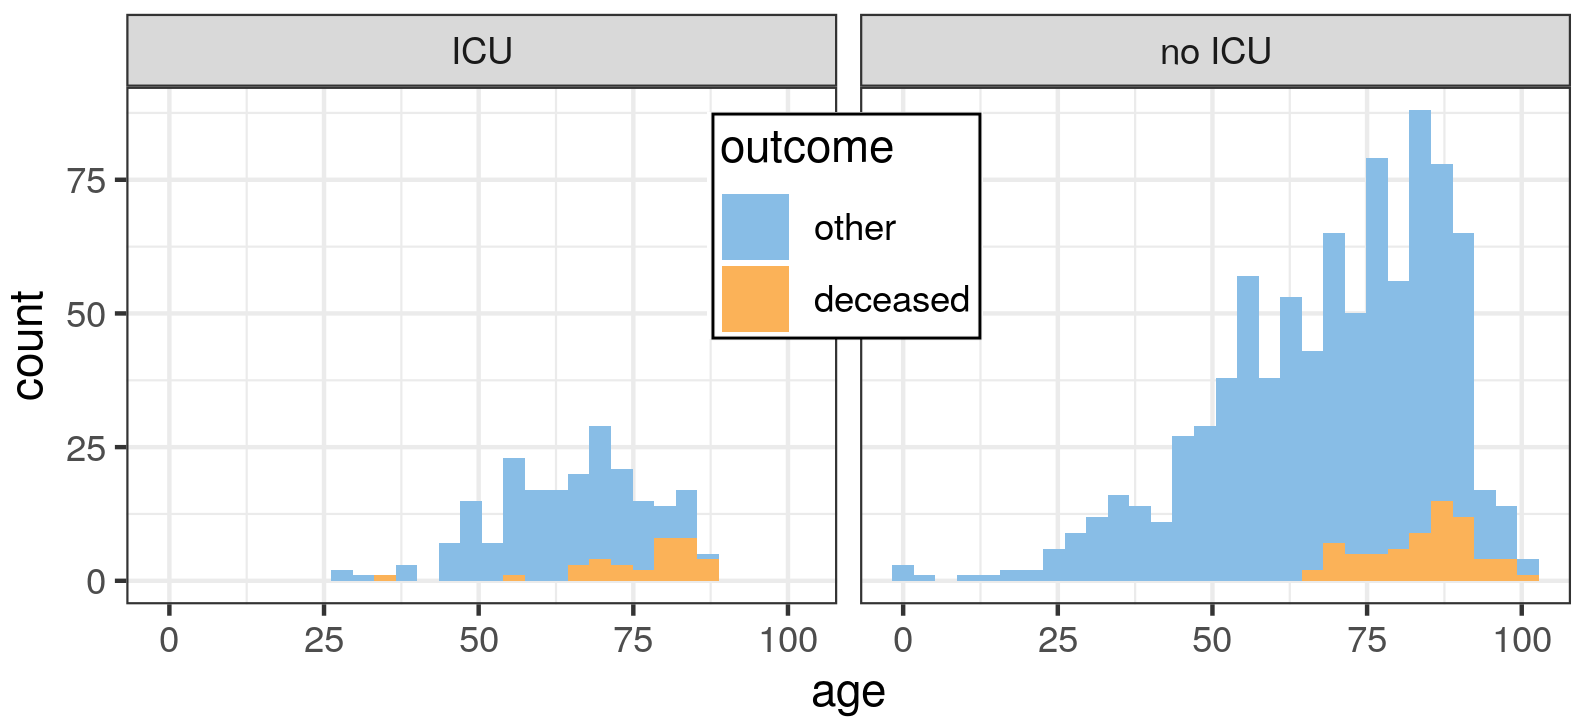
\includegraphics{fig_covid-switzerland-npi/fig_supp/VD_hist_age_mod.png}
    \label{fig:vdage}
\end{figure}
\begin{figure}[!htb]
    \centering
    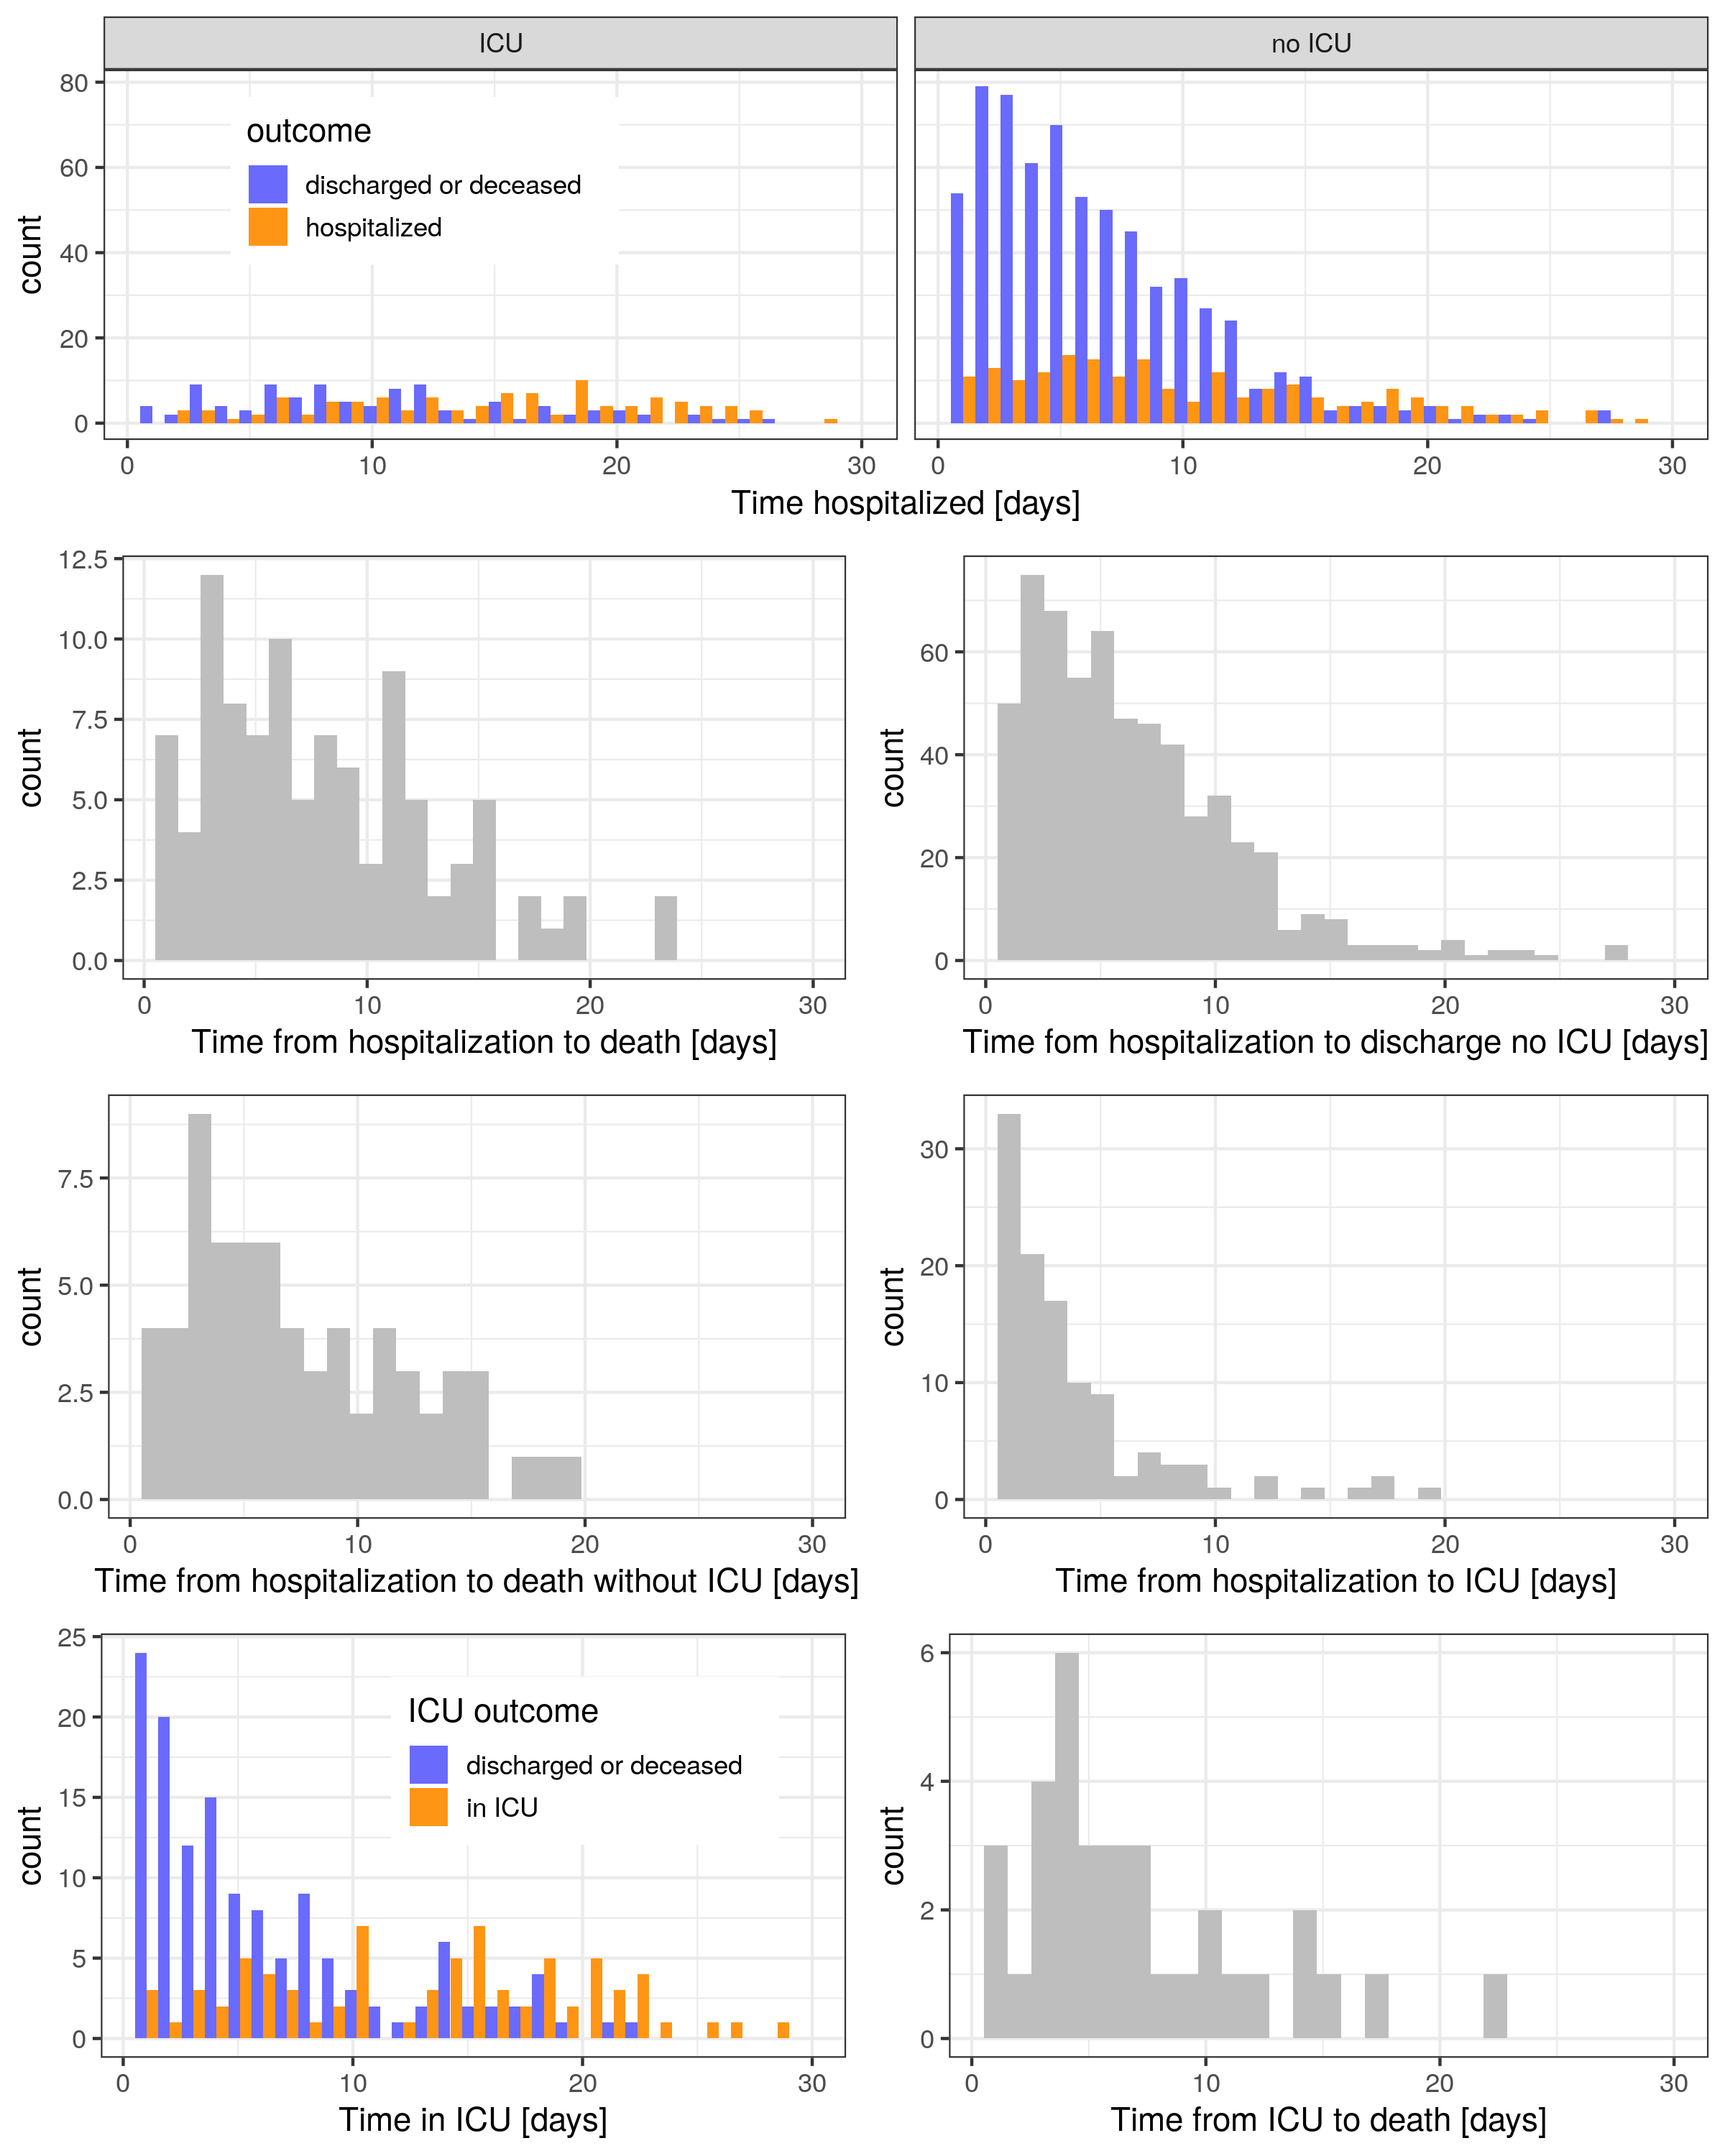
\includegraphics{fig_covid-switzerland-npi/fig_supp/VD_times.png}
    \caption[Key data of hospitalization events in canton de Vaud]{Data from canton de Vaud showing times to key hospitalization events. In order to perform this analysis, the patients are splitted in two categories: those who did not go through ICU during their stay and those who did. From left to right, top to bottom: total length of hospital stay for patients that went to ICU, then similarly for patient that did not. Then the time to death is shown for all patients, followed by both the time to discharge and to death for non-ICU patients. The last three graphs concerns ICU patients and detail ICU focused estimate: time from hospitalization to ICU, time in ICU and time from ICU to death. When meaningful, both currently hospitalized patient (orange) and already out-of-hospital patients (blue) are shown.}
    \label{fig:vdtimes}
\end{figure}

Of 777 patients with a known outcome on April 14, 104 died (13\%). The hospitalized Case Fatality Ratio (hCFR) is estimated by adjusting for the distribution of time hospitalization to death accounting for the fact that outcomes have not been yet observed for all patients (right-censoring\footnote[][-2\baselineskip]{The dataset presented here is two weeks more recent than the one visible in the example scenario planning report for Canton de Vaud (see Results, \textsc{Chapter 4}). It takes into account 137 additional patients, and the comparison with fig.~\ref{fig:vdage} strikingly shows how the distribution changes as the system is observed longer.}). To account for multiple outcomes (death and discharge), a parametric competing risk survival model is implemented\cite{Ghani:MethodsEstimatingCase:2005}. A Bayesian approach is choosen\cite{Bellot:TreebasedBayesianMixture:2018}, that enables us to fit parametric distributions to times to events using accelerated failure models. This method allows for the joint estimation of the probability of each event type and the distributions of times to events. In this case the probability of death, i.e. the hCFR. A \textsc{covid}-19 modeling study in France identified mixtures of probabilities of times to death, with a group dying faster with exponentially-distributed times and one dying slower\cite{Salje:EstimatingBurdenSARSCoV2:2020}. The Bayesian survival framework is extended to test for mixture in times to death and recovery. Model patients being discharged from ICU and subsequently dying, which was the case for 4/138 patients with known outcome, are not taken into account. Neither are accounted for multiple ICU stays per patient since this information was not available. Both Gamma and Log-Normal distributions are fitted separately to patients that did not go into ICU, and patients that did. For the former, it is modeled times from hospitalization to death or discharge, and for the latter times from ICU entry to both outcomes. Models were fit with Stan\cite[-5\baselineskip]{Carpenter:StanProbabilisticProgramming:2017}, and selection was done using Bayesian leave-one-out cross-validation\cite[-2.5\baselineskip]{Vehtari:PracticalBayesianModel:2017}. \\
\begin{figure}[!htb]
    \centering
        \caption[Survival functions of death and discharge for hospitalized patients and patients in ICU][-8\baselineskip]{Survival functions of death and discharge for hospitalized patients and patients in ICU. The lines represent the mean estimated cumulative probability of dying (full) and 1 minus the cumulative probability of discharge (dotted) estimated with non-parametric (Aalen-Johansen estimator, shading gives the 95\% CI) and parametric (assuming gamma and log-normal distributions, shading indicate the 95\% CrI) methods. Time is in days from hospitalization for patients that did not require ICU, and time from ICU admission for those that did. The point at which the lines join represents the probability that the final outcome is death, which was estimated to be 28.1\% (95\% CrI: 16.4-40.9) for patients in ICU and 13.0\% (95\% CrI: 9.9-16.6) for patients not requiring ICU based on the log-normal distribution.}
    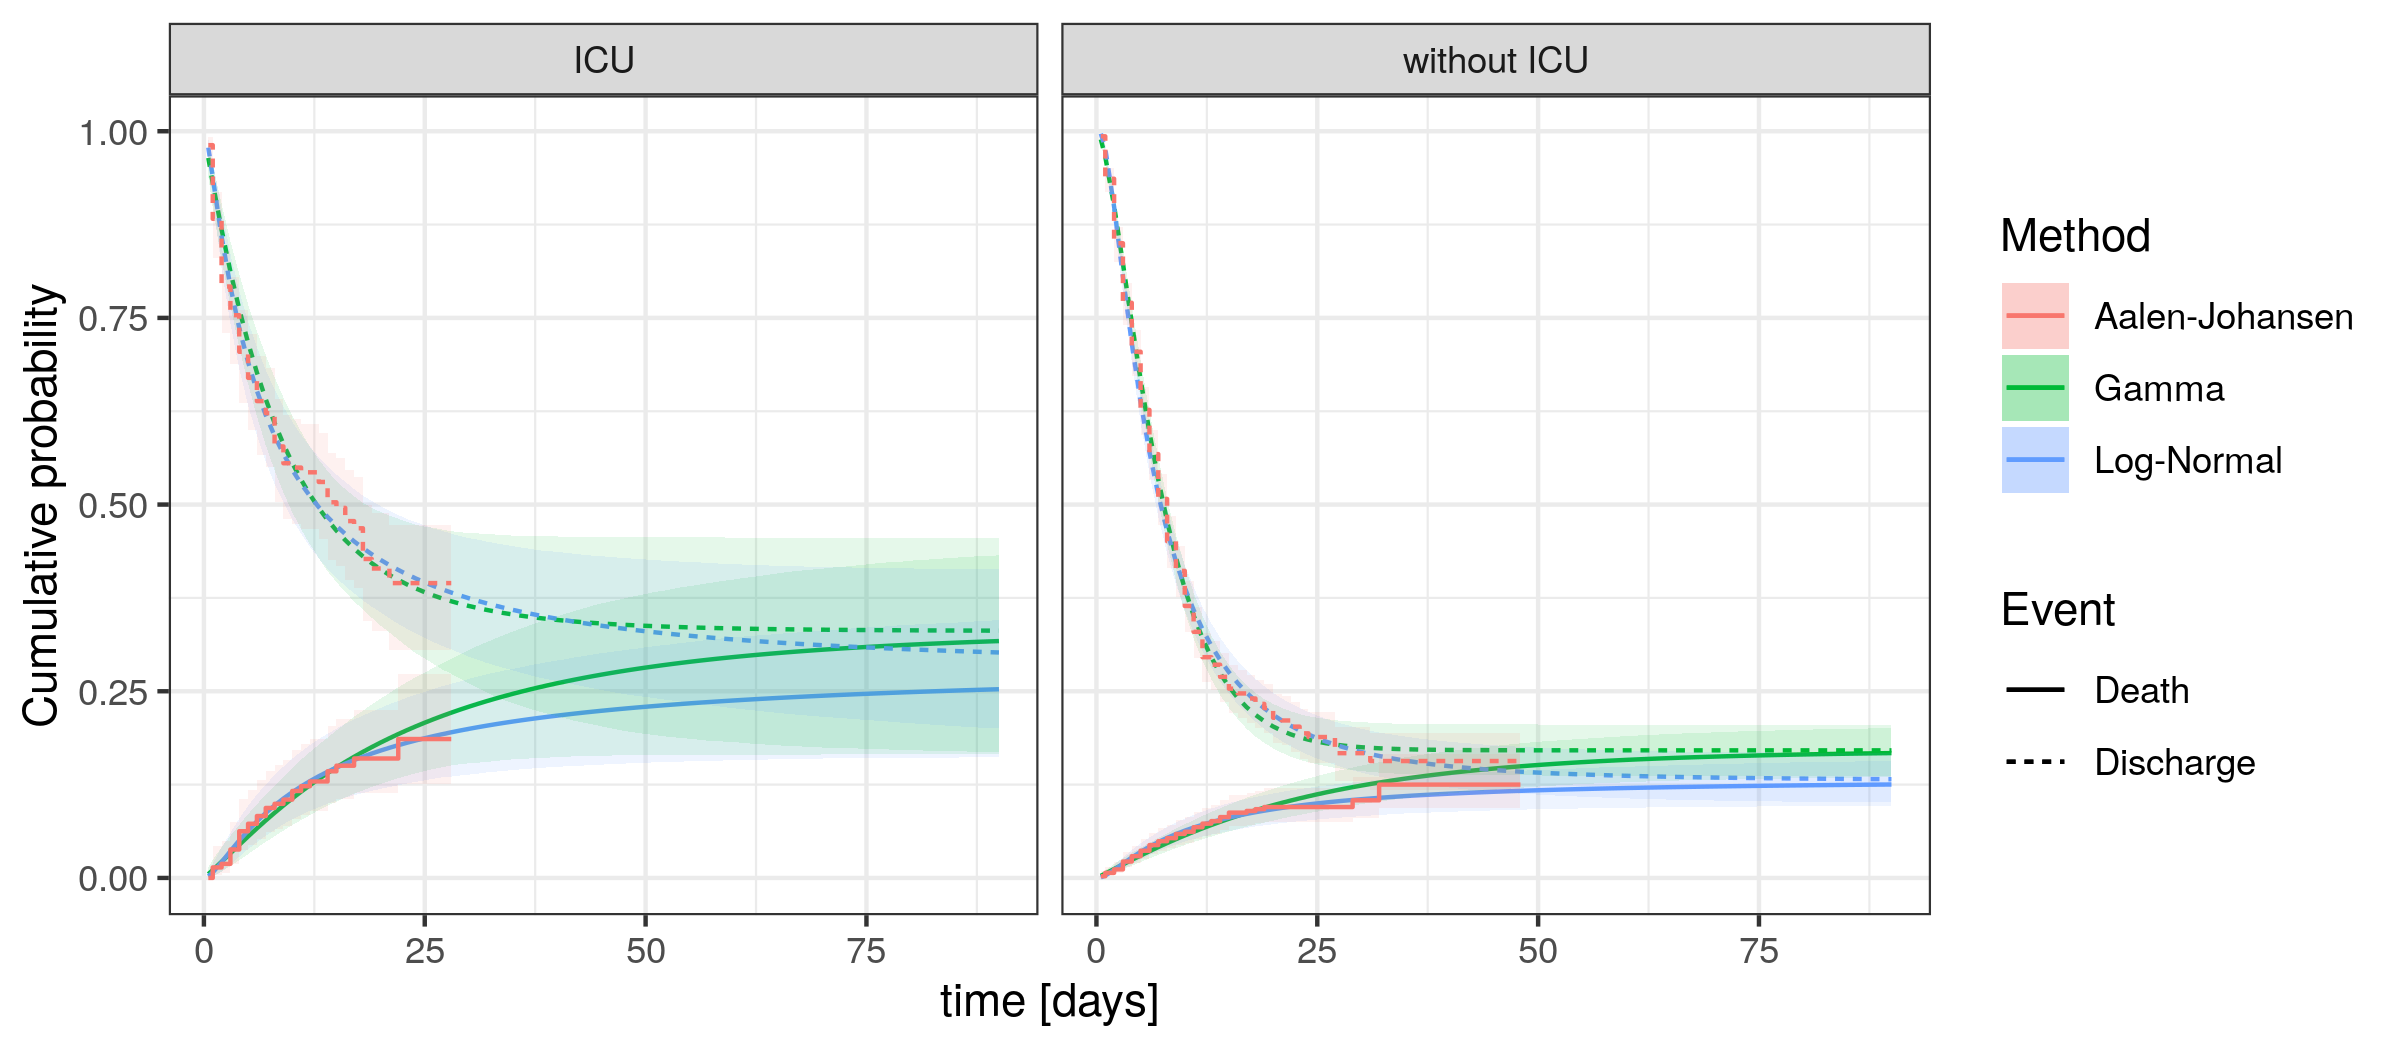
\includegraphics{fig_covid-switzerland-npi/fig_supp/survival_analaysis.png}
    \label{fig:delays}
\end{figure}


Times to death and discharge were best described by log-normal distributions with a single group both for patients having required ICU or not (fig.~\ref{fig:delays}). When accounting for right-censoring and assuming log-normally distributed times to events, an overall hCFR is estimated at 16.0\% (95\% credible interval, CrI: 12.5-19.8), resulting from a hCFR of 28.1\% (95\% CrI: 16.4-40.9) for patients requiring ICU and 13.0\% (95\% CrI: 9.9-16.6) for patients that did no require it. Estimated hCFRs were slightly higher when assuming gamma-distributed times to events (overall hCFR of 20.3\%, 95\% CrI: 15.9-24.1). The distribution of times of hospitalization processes are shown in fig.~\ref{fig:vdtimes}, and fitted distribution parameters given in tab.~\ref{tab:vdparams}.

\begin{table}[t]
\caption[Observed hospitalization time distributions]{Observed hospitalization time distributions. All times are in days and taken from the date of hospitalization if not specified otherwise. Note that these estimates are biased due to right-censoring of observations and probably under-estimate the true distributions. Estimates that account for right-censoring are shown in tab.~\ref{tab:survpars}.}
\label{tab:vdparams}
\centering
\begin{tabular}{lrrrr}
\toprule
 & mean & sd & mean (logscale) & sd (logscale)\\
\midrule
Time hospitalized & 8.49 & 6.58 & 1.81 & 0.87\\
Time to death & 8.23 & 6.09 & 1.80 & 0.87\\ \addlinespace
Time to discharge without ICU & 6.29 & 4.66 & 1.56 & 0.80\\
Time hospitalized without ICU & 7.35 & 5.79 & 1.68 & 0.85\\
Time to death without ICU & 7.84 & 6.27 & 1.73 & 0.88\\ \addlinespace
Time to ICU & 2.35 & 3.79 & 0.18 & 1.05\\
Time hospitalized with ICU & 13.14 & 7.50 & 2.37 & 0.72\\
Time in ICU & 8.36 & 6.76 & 1.69 & 1.04\\
Time from ICU to discharge & 8.68 & 6.99 & 1.71 & 1.07\\
Time from ICU to death & 6.97 & 4.98 & 1.68 & 0.77\\
\bottomrule
\end{tabular}
\end{table}


\begin{fwtable}
    \centering
    \begin{tabular}{ccccccc}
\toprule
 & & \multicolumn{3}{c}{Log-Normal} & \multicolumn{2}{c}{Gamma}\\ \cmidrule(rl){3-5} \cmidrule(rl){6-7}
Group & Event & median & mean-log & SD-log & scale & shape\\
\midrule
Without ICU & Death & 10 (7.3--16) & 2.3 (2--2.8) & 1.2 (0.95--1.5) & 21 (21--22) & 1.1 (0.83--1.4)\\
 & Discharge & 6.1 (5.6--6.6) & 1.8 (1.7--1.9) & 0.93 (0.87--0.99) & 4.3 (4.4--4.2) & 1.8 (1.6--2)\\ \addlinespace
ICU & Death & 13 (6.2--30) & 2.6 (1.8--3.4) & 1.3 (0.87--1.9) & 21 (12--23) & 1.2 (0.74--1.9)\\
 & Discharge & 6.4 (4.3--9.3) & 1.8 (1.5--2.2) & 1.3 (1.1--1.6) & 9.1 (8.1--11) & 1 (0.75--1.4)\\
\bottomrule
\end{tabular}
\caption[Estimated parameters of hospitalization time distributions]{Estimated parameters of hospitalization time distributions. These estimates differ from observed values given in tab.~\ref{tab:vdparams} by accounting for right-censoring of observations. Time from hospitalization to discharge or death, and from ICU admission to discharge or death are reported here. Estimates were obtained using competing risk survival model as described above. Parameters are given in terms of their posterior mean and 95\% CrI (in parenthesis). For the log-normal distribution the parameters correspond to the mean and SD of the logarithm of the distribution.}
     \label{tab:survpars}
\end{fwtable}

%We build a \textsc{covid}-19 compartmental transmission model based on the Susceptible Exposed Infected Recovered (SEIR) template with three I compartments. The schematic with the different transitions and compartments is shown in SM Fig.~\ref{fig:diagram}. Infected individuals have some probability of developing severe symptoms which require hospitalization after a delay from symptom onset ($I_h$). Hospitalization can lead to recovery or death, either through normal hospitalization ($H_{s}$ and $H_d$ respectively) or passing through Intensive Care Units (ICUs) ($U_{s}$ and $U_d$ respectively). Data from the canton of Vaud show a high proportion of deaths outside of hospitals ($\approx 50\%$), we therefore also include a pathway from infection to death without passing through hospitalization ($I_d$). 


%The time spent in the observable hospitalization states were used to define the number of stages in each compartment by fitting Erlang distributions to the data of canton de Vaud. To account for right-censoring we do not fit directly to observed times to events but rather to the estimated log-normal distributions described in the survival analysis section above. We fit the rate parameter of the Erlang distributions for shape parameters between 1 and 10 by minimizing the Kullback-Leibler (KL) divergence between the Erlang and estimated log-normal distributions. The final fit was taken to be the one with the smallest KL-divergence. \\


%\section{Model equations}\label{sec:stoch}
%As in \textsc{Chapter 2} and 3, the model is implemented as a discrete-state model based on a Partially-Observed Markov Process (POMP), or equivalently a Hidden Markov Model (HMM), simulating the transitions between compartments as discrete events using stochastic count processes\cite{King:InapparentInfectionsCholera:2008,Breto:TimeSeriesAnalysis:2009}. Let \(N_{AB}(t)\) be the number of individuals transiting between compartments \(A,B\in \mathcal{X}\) in the time interval \([0,t)\)  where $\mathcal{X}$ is the state vector,
%$$\mathcal{X} = \{S, E, I_{1,2,3} , I_d, I_h, H_{s}, H_{d}, H_{u}, U_{s}, U_{d}, R, D\}$$
%
%Using the same notation as previous chapters, the number of transitions during a time-step $\Delta t$ is
%\(\Delta N_{AB}(t) = N_{AB}(t+\Delta t) - N_{AB}(t)\). We model time-varying $R_0(t) = \beta(t)/(3r_I)$ as a geometric random walk defined by its calibrated variance, where $\beta$ is the transmission parameter and $1/(3r_I)$ is the mean duration spent in the infectious compartments $I_1$ to $I_3$. The force of infection is expressed in terms of $\beta(t)$ in the model. Given the state of the system at time \(t\), \(\mathcal{X}_t\), the model reads:
%\begin{gather}
%\label{eq:stochsys}
%\begin{aligned}
%    \mathbb{P}\left[ \Delta N_{SE}(t) = 1 \right|\mathcal{X}_t] &=  \beta(t)  \frac{I_1(t) + I_2(t) + I_3(t)}{P} S(t) \Delta t + o(\Delta t)\\
%    \mathbb{P}\left[ \Delta N_{EI_1}(t) = 1 \right|\mathcal{X}_t] &= r_{E} E(t) \Delta t + o(\Delta t) \\
%    \mathbb{P}\left[ \Delta N_{I_1 I_2}(t) = 1 \right|\mathcal{X}_t] &= 3r_{I} I_1(t) \Delta t + o(\Delta t)\\
%    \mathbb{P}\left[ \Delta N_{I_2 I_3}(t) = 1 \right|\mathcal{X}_t] &= 3r_{I} I_2(t) \Delta t + o(\Delta t)\\
%    \mathbb{P}\left[ \Delta N_{I_3 I_d}(t) = 1 \right|\mathcal{X}_t] &= p_{I_d|I_3} \cdot 3r_{I}  I_3(t) \Delta t + o(\Delta t)\\
%    \mathbb{P}\left[ \Delta N_{I_3 I_h}(t) = 1 \right|\mathcal{X}_t] &= p_{I_h|I_3} \cdot 3r_{I}   I_3(t) \Delta t + o(\Delta t)\\
%    \mathbb{P}\left[ \Delta N_{I_3 R}(t) = 1 \right|\mathcal{X}_t] &= p_{R|I_3} \cdot 3r_{I}  I_3(t) \Delta t + o(\Delta t)\\
%    \mathbb{P}\left[ \Delta N_{I_d R}(t) = 1 \right|\mathcal{X}_t] &= p_{R|I_d} \cdot r_{I}  I_d(t) \Delta t + o(\Delta t)\\
%    \mathbb{P}\left[ \Delta N_{I_d D}(t) = 1 \right|\mathcal{X}_t] &= p_{D|I_d}\cdot r_{I} I_d(t) \Delta t + o(\Delta t)\\
%    \mathbb{P}\left[ \Delta N_{I_h H_d}(t) = 1 \right|\mathcal{X}_t] &= p_{H_d|I_h} \cdot r_{I_h}  I_h(t) \Delta t + o(\Delta t)\\
%    \mathbb{P}\left[ \Delta N_{I_h H_u}(t) = 1 \right|\mathcal{X}_t] &= p_{H_u|I_h} \cdot r_{I_h} I_h(t) \Delta t + o(\Delta t)\\
%    \mathbb{P}\left[ \Delta N_{I_h H_s}(t) = 1 \right|\mathcal{X}_t] &= p_{H_s|I_h} \cdot r_{I_h} I_h(t) \Delta t + o(\Delta t)\\
%   \mathbb{P}\left[ \Delta N_{H_s R}(t) = 1 \right|\mathcal{X}_t] &=  r_{H_s} H_s(t) \Delta t + o(\Delta t)\\
%    \mathbb{P}\left[ \Delta N_{H_u U_d}(t) = 1 \right|\mathcal{X}_t] &=   p_{U_d|H_u} \cdot r_{H_u} H_u(t) \Delta t + o(\Delta t)\\
%    \mathbb{P}\left[ \Delta N_{H_u U_s}(t) = 1 \right|\mathcal{X}_t] &=   p_{U_s|H_u} \cdot r_{H_u} H_u(t) \Delta t + o(\Delta t)\\
%    \mathbb{P}\left[ \Delta N_{H_d D}(t) = 1 \right|\mathcal{X}_t] &=   r_{H_d} H_d(t) \Delta t + o(\Delta t)\\
%    \mathbb{P}\left[ \Delta N_{U_s R}(t) = 1 \right|\mathcal{X}_t] &=   r_{U_s} U_s(t) \Delta t + o(\Delta t)\\
%    \mathbb{P}\left[ \Delta N_{U_d D}(t) = 1 \right|\mathcal{X}_t] &=   r_{U_d} U_d(t) \Delta t + o(\Delta t)\\
%\end{aligned}
%\end{gather}
%
%\noindent assuming that \(\mathbb{P}[\Delta N_{XY} > 1|\mathcal{X}_t] = o(\Delta t) \; \forall X,Y \in \mathcal{X}\). Branching probabilities from stage $X$ to $Y$ are noted $p_{Y|X}$ and rates of stay in stage $X$ is noted $r_X$.
%The ensuing stochastic variations of the state variables are:
%\begin{gather}
%\label{eq:stochstates}
%\begin{aligned}
%    \Delta E(t) &= \Delta N_{SE}(t) - \Delta N_{EI_1}(t))\\
%    \Delta I_1(t) &= \Delta N_{EI_1}(t) - \Delta N_{I_1 I_2}\\
%    \Delta I_2(t) &= \Delta N_{I_1 I_2} - \Delta N_{I_2 I_3}\\
%    \Delta I_3(t) &=  \Delta N_{I_2 I_3} - \Delta N_{I_3 I_d} - \Delta N_{I_3 I_h} -  \Delta N_{I_3 R}\\
%    \Delta I_d(t) &= \Delta N_{I_3 I_d} - \Delta N_{I^d R} - \Delta N_{I^d D}\\
%    \Delta I_h(t) &= \Delta N_{I_3 I_h} -  \Delta N_{I_h H_d} -  \Delta N_{I_h H_u} -  \Delta N_{I_h H_s} \\
%    \Delta H_s(t) &= \Delta N_{I_h H_s} -  \Delta N_{H_s R}\\
%   \Delta H_d(t) &= \Delta N_{H_s H_d} -  \Delta N_{H_d D}\\
%    \Delta H_u(t) &= \Delta N_{I_h H_u} - \Delta N_{H_u U_d} - \Delta N_{H_u U_a} - \Delta N_{H_u U}\\
%    \Delta U(t) &=  \Delta N_{H_u U} - \Delta N_{U R}\\
%    \Delta U_d(t) &=  \Delta N_{H_u U_d} - \Delta N_{U_d D}\\
%    \Delta D(t) &=  \Delta N_{I^d D} + \Delta N_{U_d D} + \Delta N_{H_d D}\\
%    \Delta R(t) &= \Delta N_{I_3 R} + \Delta N_{I^d R} +  \Delta N_{H_s R} + \Delta N_{U R} \\
%     S(t) &= P - \sum_{X \in \mathcal{X} \backslash \{S\}} X(t),
%\end{aligned}
%\end{gather}
%where the equation for \(S(t)\) enforces a constant total population. The total population for each canton and for Switzerland is taken from the 2018 estimate of the Federal Statistical Office\cite{Officefederaldelastatistique:Population:2018}.
%
%
%\section{Model Parameters}
%Rates of transitions are shown Table~\ref{parRates} and branching probabilities in Table~\ref{parProb}. Proper indentifiability is needed to capture the dynamics of $R_0$ so most of the parameters where fixed to values of the litterature.
%The model is parameterized conditioning on a mean generation time of 5.2 days \parencite{Ganyani:EstimatingGenerationInterval:2020}, and an exposed and non-infectious duration of 2.9 days \parencite{He:TemporalDynamicsViral:2020}, yielding a mean duration of 4.6 days in the infectious compartments. All rates are given in day$^{-1}$ and the subscript subscript in the parameter names indicate the compartment from which exits happen at the given rate.
%
%
%\begin{table*}[ht!]
%\centering\small
%\begin{tabular}{lccl} 
%\toprule
%Rate & Source & Value or starting bound & Corresponding duration  \\
%\midrule
%$r_{E}$ & \parencite{He:TemporalDynamicsViral:2020} & $1/2.9$& infected but non-infectious state \\
%$r_{I}$ & \parencite{He:TemporalDynamicsViral:2020, Ganyani:EstimatingGenerationInterval:2020}  & $1/4.6$  & infectious state\\
%$r_{I_h}$ & \parencite{Scire:ReproductiveNumberCOVID19:2020} & $1/1.6$& end of the infectious period to hospitalization \\
%$r_{H_s}$ & Vaud data & $1/7.6$ & hospitalization to discharge \\
%$r_{H_d}$ & Vaud data & $1/23.7$ & hospitalization to death \\
%$r_{H_u}$ & Vaud data & $1/2.35$  & hospitalization to ICU admission \\
%$r_{U_s}$ & Vaud data & $1/9.3$  & ICU admission to discharge \\
%$r_{U_d}$ & Vaud data & $1/25.6$ & ICU admission to death \\
%$r_{I_d}$ & Fitted & $1/50 - 1/1$ &end of the infectious period to death when not hospitalized \\
%\bottomrule
%\end{tabular}
%\caption[Transition rates from each compartment of the model]{Transition rates from each compartment of the model. Compartments $I_{1,2,3}$ are composed of several stages so the rate of exit from each one is $3r_{I}$. }
%\label{parRates}
%\end{table*}
%
%There are seven different pathways from susceptible to either death or recovery. It is assumed that the proportion of severe infections that have severe symptoms which would require hospitalization is of 7.5\% \parencite{Verity:EstimatesSeverityCoronavirus:2020}, that 50\% of deaths happen outside of hospitals (data from cantons of Vaud as above and Geneva from OpenZH), that the hospitalized case fatality ratio is of 16\% (data from canton of Vaud, see above), the probability of going into ICU for hospitalized patients is of 20\% (data from canton of Vaud), and an population-level infection fatality ratio (IFR) of 0.75 \% which is in the range of published estimates\parencite{Verity:EstimatesSeverityCoronavirus:2020,Russell:EstimatingInfectionCase:2020}.
%\begin{table*}[ht!]
%\centering\small
%\begin{tabular}{lccl} 
%\toprule
%Parameter & Source & Value &  Description \\
%\midrule
%IFR & Assumed & 0.0075 & Infection fatality ratio \\
%$p_s$ & Assumed &  0.075 & Probability of severe symptoms\\
%$p_h$ &  Vaud data $|$ IFR &  0.31 & Probability of hospitalization given severe symptoms  \\
%$p_{I_d|I_3}$ & Vaud data $|$ IFR, $p_s$ & $p_s (1-p_h)$&  Probability of death outside of the hospital given sever symptoms  \\
%$p_{I_h|I_3}$ & Vaud data $|$ IFR, $p_s$  & $p_s p_h$   &  Probability of hospitalization given infection \\
%$p_{R|I_3}$   & Deduced  $|p_s$ & $(1-p_s)$    &  Probability of not having sever symptoms\\
%$p_{D|I_d}$   & Vaud data $|$ IFR, $p_s$  &  0.073   &  Probability of death given severe symptoms and not hospitalized \\
%$p_{R|I_d}$   & Vaud data $|$ IFR, $p_s$ &  $1-p_{D|I_d}$   & Probabilitys of recovery given severe symptoms \\
%$p_{H_s|I_h}$ & Vaud data &  0.72   &  probability of discharge without ICU given hospitalization\\
%$p_{H_d|I_h}$ & Vaud data &  0.11    &  Probability of death given not going into ICU\\
%$p_{H_u|I_h, !H_s}$ & Vaud data &  0.61   &  Probability of ICU given not discharged without ICU\\
%$p_{U_d|H_u}$ & Vaud data & 0.28   &  Probability of death given ICU \\
%\bottomrule
%\end{tabular}
%\caption[Branching probabilities of the model]{Branching probabilities of the model. The probability of transition from stage $A$ to stage $B$ is $p_{B|A}$. }
%\label{parProb}
%\end{table*}
%
%
%\section{Assessment of Model Fit}
%In fig. \ref{fig:chfit} and fig. \ref{fig:cantonfit}, model fits at respectively the national and cantonal levels are showed. Note that the hospitalization processes in all cantons and at the national level were parameterized with data from the canton de Vaud. Difference in hospital protocols and procedures in each canton as well as transfers of patient between cantons cause differences between observed and modelled ICU occupancy. This model tends to overestimate current ICU using time distributions from canton de Vaud, while death (cumulative and incidence) and current hospitalization are well captured. 
% 
%\begin{figure}[!htb]
%    \centering
%    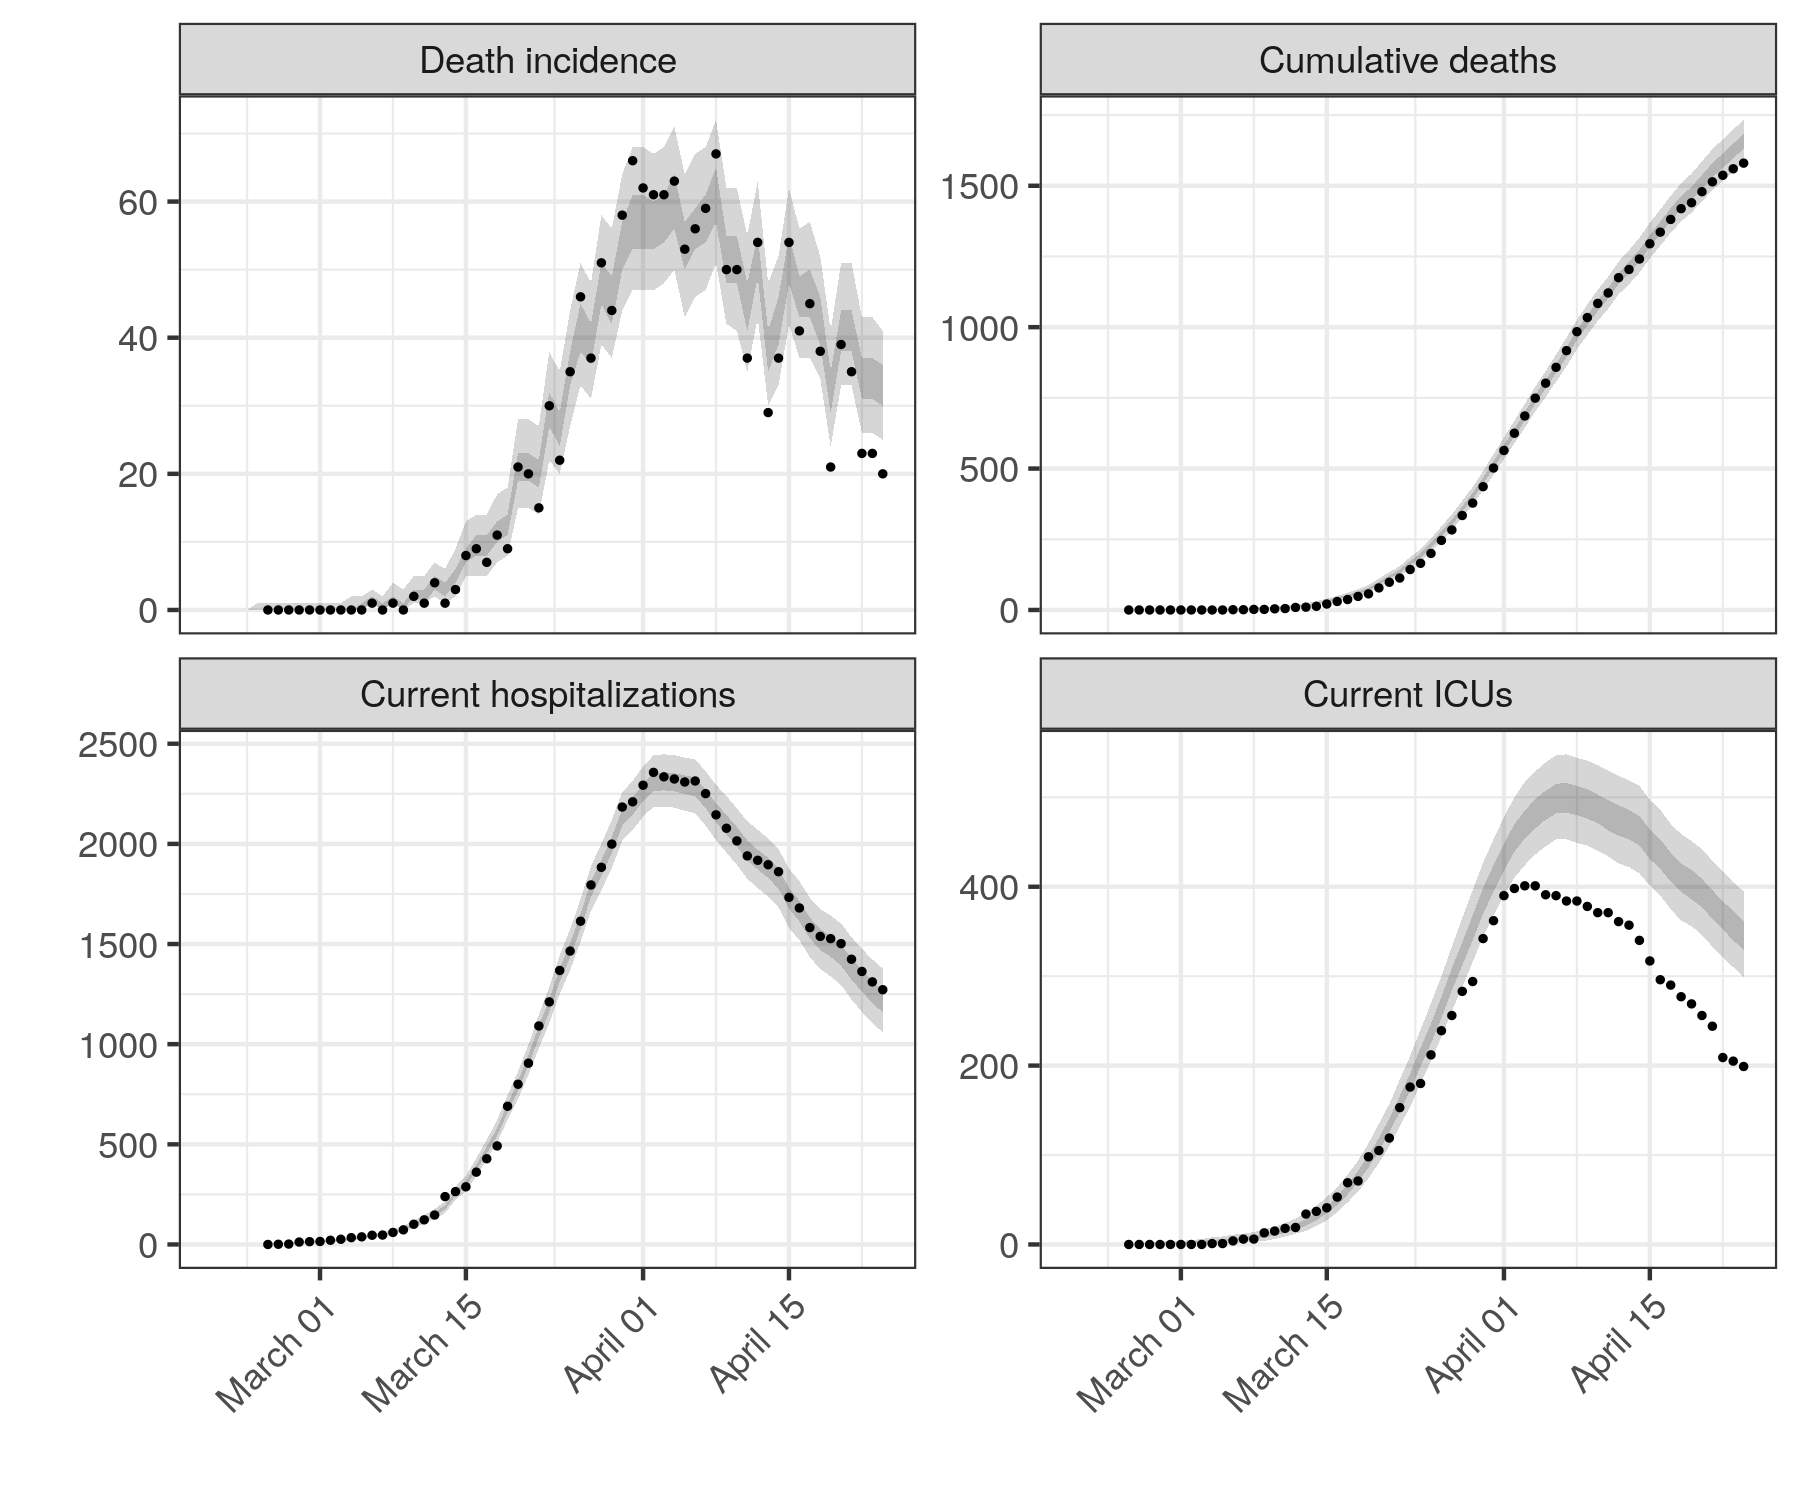
\includegraphics{fig_covid-switzerland-npi/fig_supp/CH_fits.png}
%    \caption[Model fit at at national level]{Model fit at at national level. Model results are given in terms of the 95\% (light gray) and 50\% quantile ranges of the smoothing distribution of R$_0$ at the maximum likelihood estimates of inferred parameters. Data (points) from \textcite{Probst:DaenuprobstCovid19casesswitzerland:2020}}.     \label{fig:chfit}
%\end{figure}
%
%\begin{figure}[!htb]
%    \centering
%    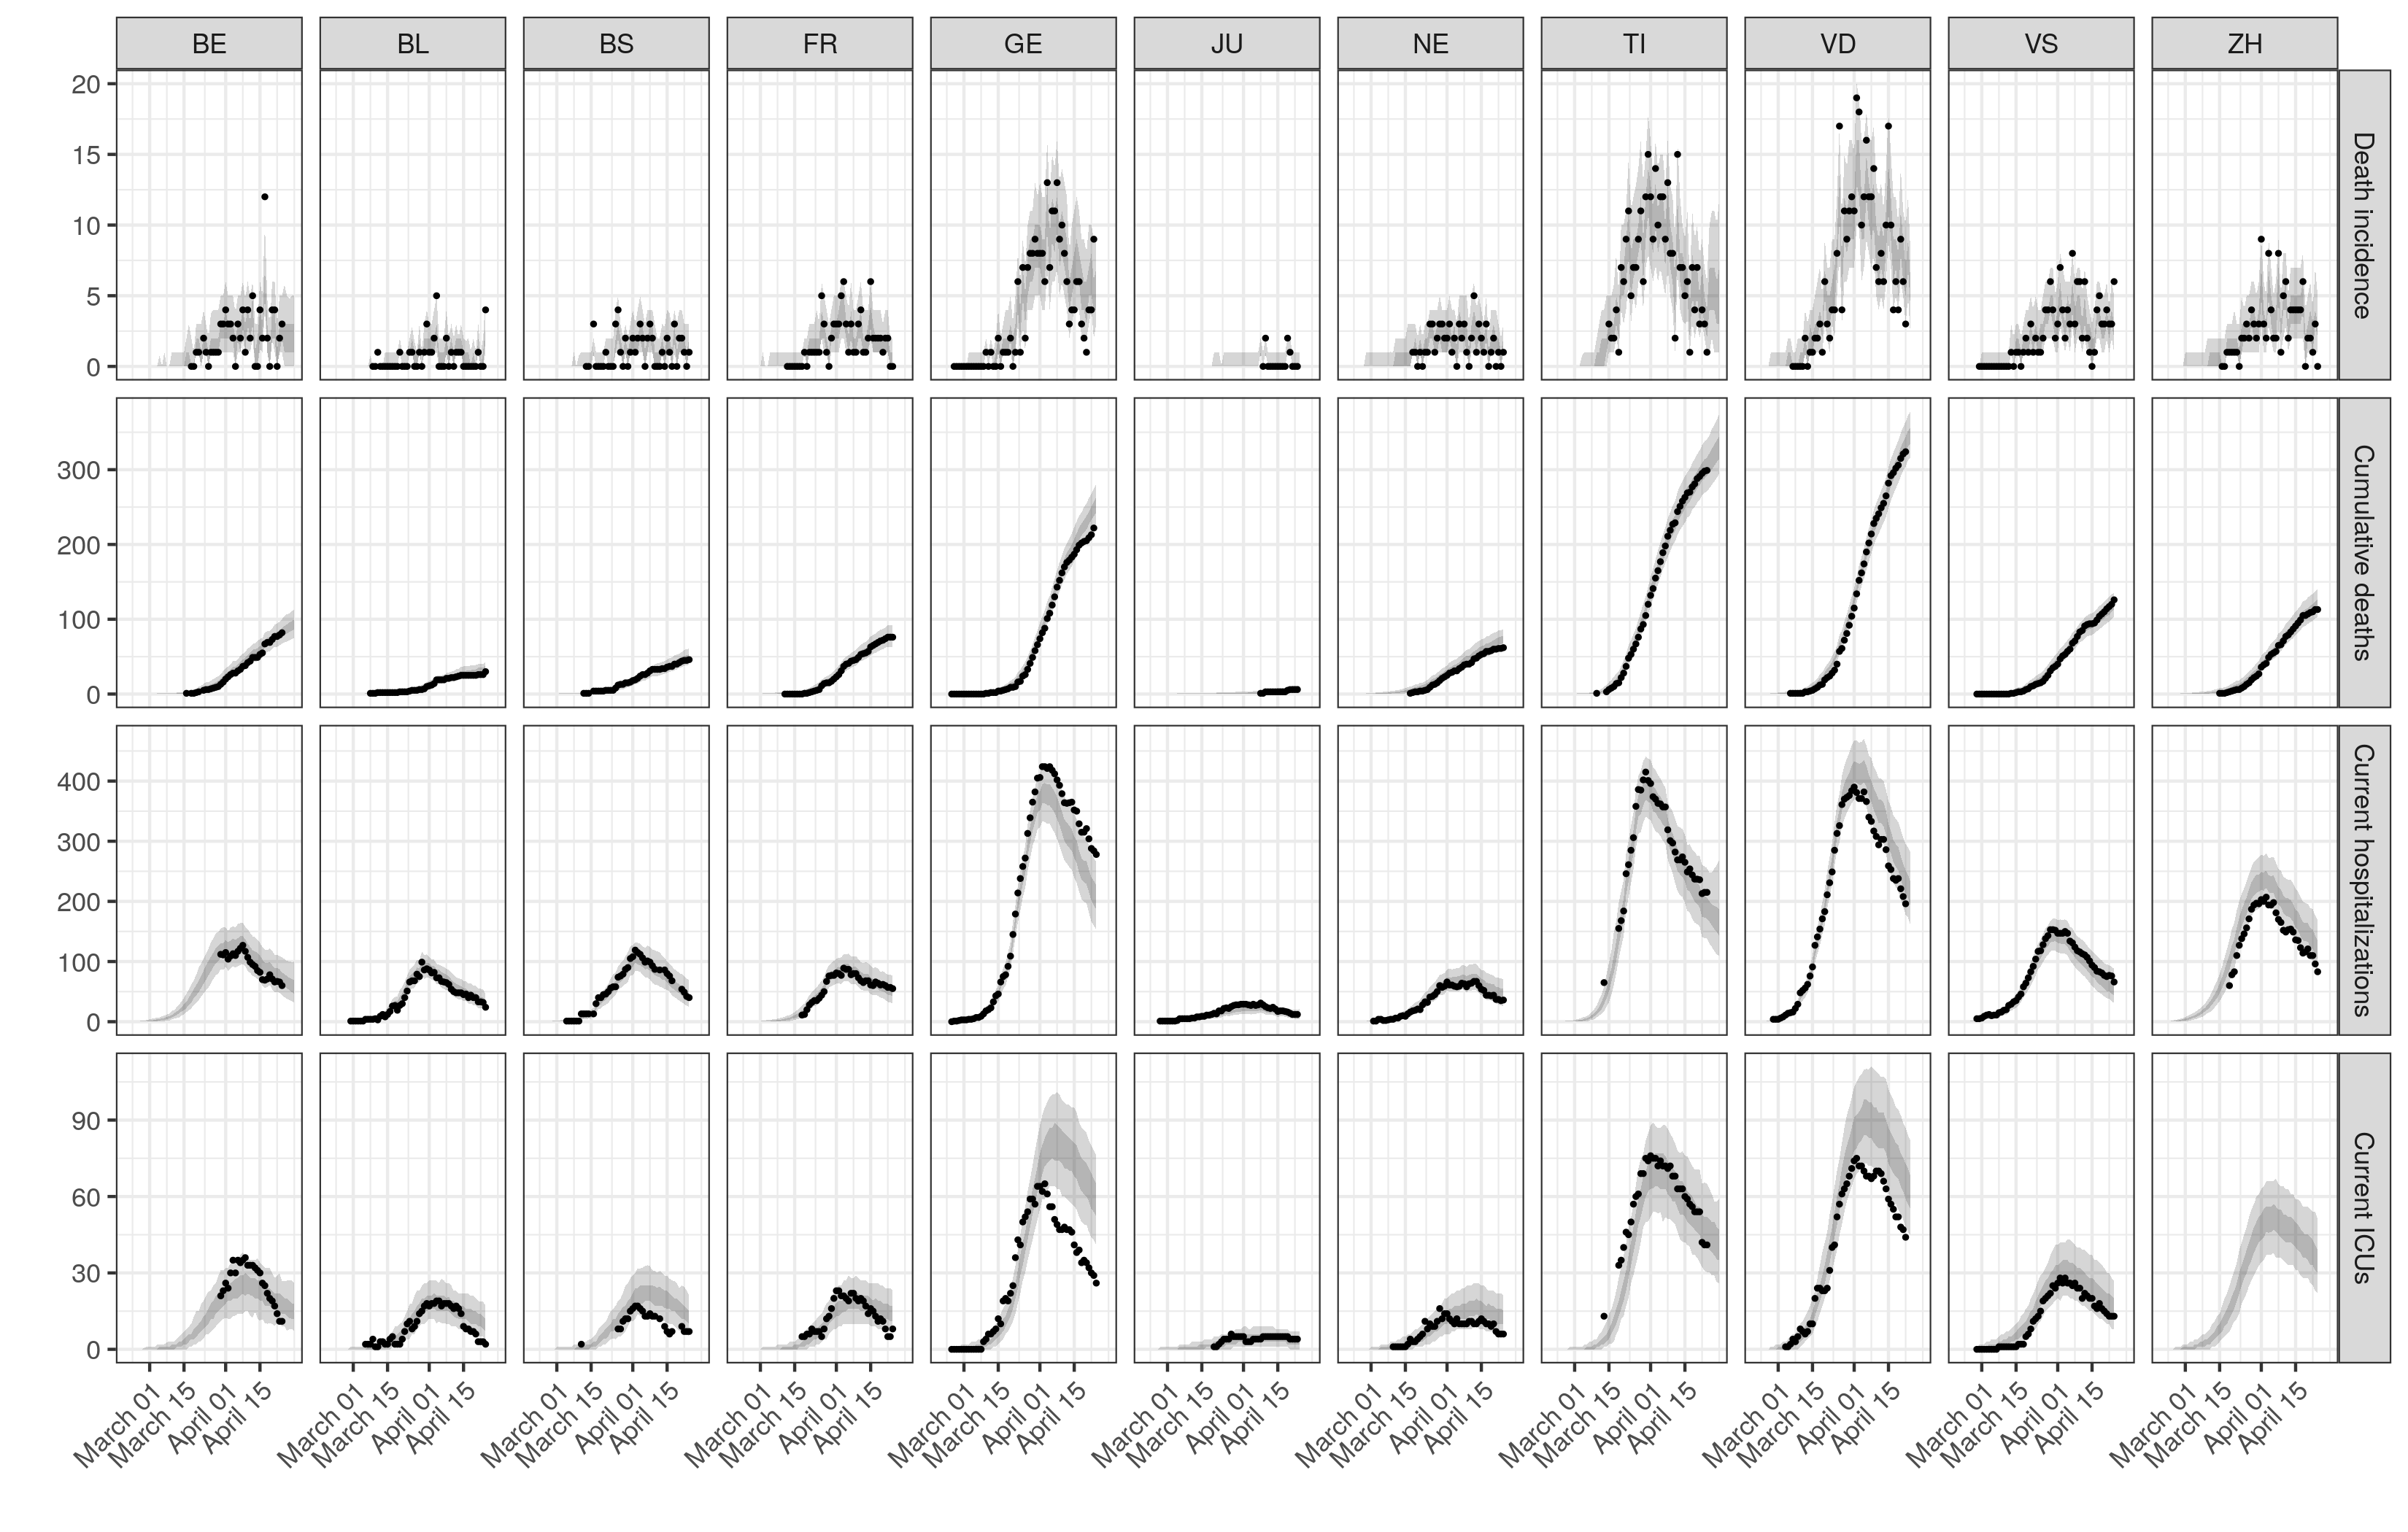
\includegraphics{fig_covid-switzerland-npi/fig_supp/caton_fits.png}
%    \caption[Cantonal level fits]{Cantonal level fits, with the same legend as in fig.~\ref{fig:chfit}. Data (points) from \textcite{openZH:OpenZHCovid19:2020}.}
%    \label{fig:cantonfit}
%\end{figure}



%\begin{figure}
%    \centering
%    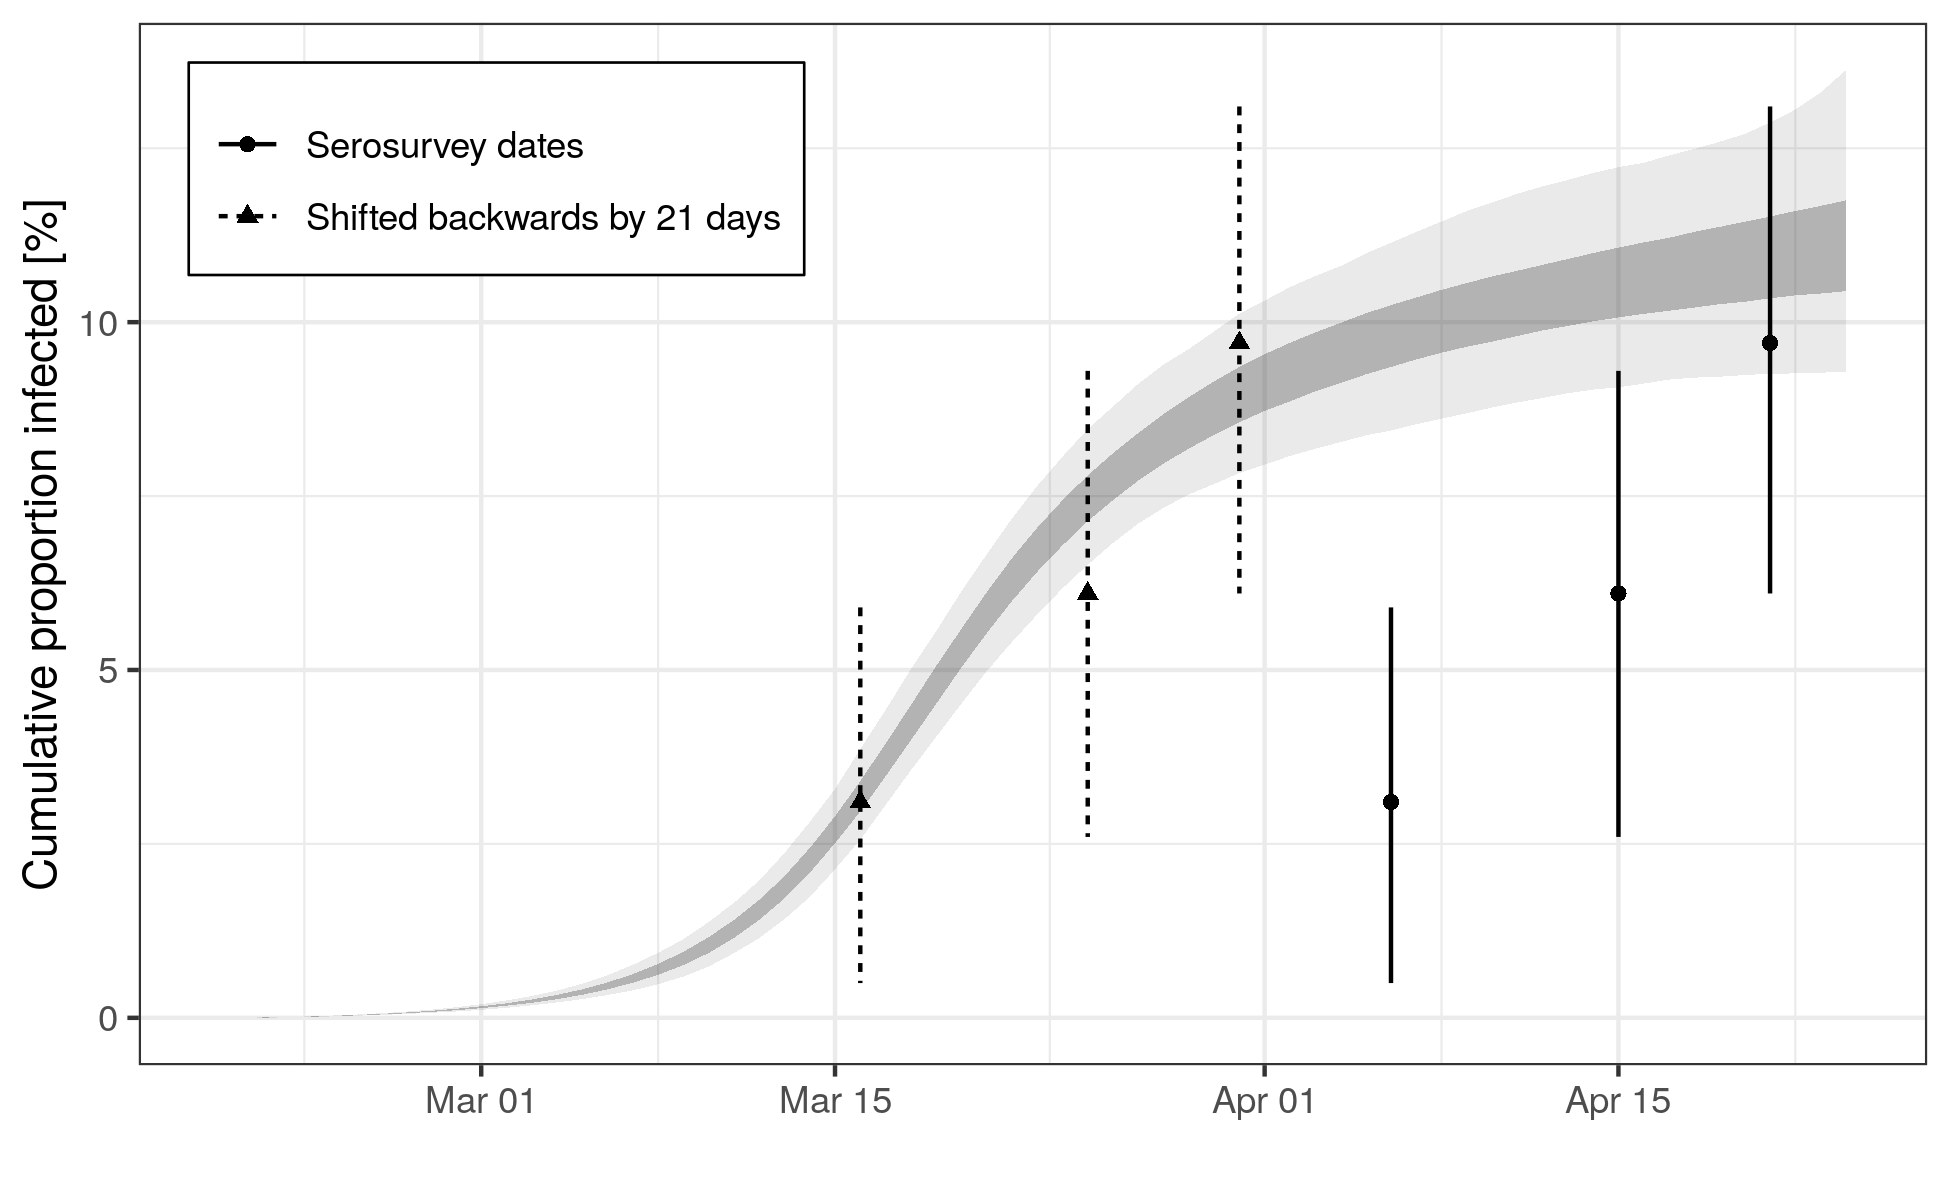
\includegraphics[width=.8\textwidth]{fig_covid-switzerland-npi/fig_supp/GE_seroprevalence_comparison.png}
%    \caption[Qualitative comparison between modelled infected in the canton of Genève and seroprevalence estimates]{Qualitative comparison between modelled proportion of people infected in the canton of Genève and seroprevalence estimates. Model estimates (ribbons, dark shading give the IQR and light shading the 95\% quantile range) are compared to seroprelavence estimates (points, error bars give the 95\% CrI)   taken from Figure 1 in \parencite{stringhini_repeated_2020} [Accessed May 15 2020]. Seroprevalence estimates do not correspond to infection status on the date of the survey due to the delay between infection and seroconversion. We roughly account for this delay by plotting seropervalence estimates shifted backwards in time to represent the delay between infection and symptom onset (6 days \parencite{bi_epidemiology_2020}) and from symptom onset to seroconversion (about 80\% of seroconversions occur within 15 days \parencite{huang_systematic_2020}), resulting in a total shift of 21 days. Note that seroprevelance estimates were not used in model fitting. Quantitative evaluation of adequacy between modelled proportion infected and seroprevalence estimates would require modelling explicitly seroconversion.}
%    \label{fig:seroprev}
%\end{figure}

%\begin{table}[]
%    \centering
%        \caption[Estimated values of R$_0$ at the beginning of the epidemic]{Estimated values of R$_0$ at the beginning of the epidemic (March 1 to March 10) and after the implementation of non-pharmaceutical interventions (March 29 to April 5). Estimates given in terms of the median and 95\% quantile range (in parenthesis).}
%
%\begin{tabular}{ccccc}
%\toprule
%\multicolumn{1}{c}{ } & \multicolumn{2}{c}{March 01-March 10} & \multicolumn{2}{c}{March 29-April 05} \\
%\cmidrule(l{3pt}r{3pt}){2-3} \cmidrule(l{3pt}r{3pt}){4-5}
% & median & 95\% QR & median & 95\% QR\\
%\midrule
%Switzerland & 2.8 & (2.5-3.1) & 0.4 & (0.27-0.6)\\
%Bern & 2.4 & (2-3) & 0.5 & (0.26-0.9)\\
%Basel-Landschaft & 2.8 & (2.2-3.7) & 0.22 & (0.03-0.7)\\
%Basel-Stadt & 3.1 & (2.6-3.8) & 0.3 & (0.13-0.6)\\
%Fribourg & 2.7 & (2.2-3.4) & 0.4 & (0.2-0.8)\\
%Geneve & 2.6 & (2.1-3) & 0.5 & (0.24-0.8)\\
%Jura & 1.4 & (1.2-1.6) & 0.7 & (0.4-1)\\
%Neuchatel & 2 & (1.7-2.3) & 0.6 & (0.4-1)\\
%Ticino & 4 & (3-5) & 0.5 & (0.29-1)\\
%Vaud & 2.7 & (2.4-3) & 0.5 & (0.3-0.8)\\
%Valais & 1.8 & (1.4-2.2) & 0.29 & (0.07-0.7)\\
%Zurich & 2.3 & (1.8-2.8) & 0.5 & (0.25-0.9)\\
%\bottomrule
%\end{tabular}
%    \label{tab:r0}
%\end{table}
%
%
%\begin{table}[]
%    \centering
%     \caption[Estimated proportion of population infected with SARS-CoV-2 as of April 24 2020]{Estimated proportion of population infected with SARS-CoV-2 as of April 24 2020. Estimates given in terms of the median and 95\% quantile range (in parenthesis).}
%\begin{tabular}{ll}
%\toprule
%Canton & Proportion infected [\%]\\
%\midrule
%Switzerland & 3.9 (3.6-4.3)\\
%Bern & 1.9 (1.4- 2.6)\\
%Basel-Landschaft & 3.9 (2.9-5.0)\\
%Basel-Stadt & 6.7 (5.0-8.6)\\
%Fribourg & 4.0 (3.0-5.4)\\
%Geneve & 11.0 (9.3-13.3)\\
%Jura & 4.2 (2.8- 6.5)\\
%Neuchatel & 6.7 (4.9-9.1)\\
%Ticino & 16.0 (13.5-21.2)\\
%Vaud & 8.0 (6.8- 9.3)\\
%Valais & 5.5 (4.4-7.4)\\
%Zurich & 2.3 (1.8- 2.9)\\
%\bottomrule
%\end{tabular}
%    \label{tab:infection}
%\end{table}

\chapter{Appendix to chapter 6}

\section{Comment on the simplifications}
\paragraph{Discussion on Simplification (a).}
Realistically, vaccinations will occur at least eight hours per day. The assumption, while justified as a computationally convenient approximation of reality, is not a priori worse than assuming that vaccine administration takes place over the whole day. More refined approximations, while in principle possible, pose severe issues because of the nature of the system dynamics. While for most initial values the system dynamics can be easily simulated with time-continuous vaccinations, the system becomes stiff by construction once almost the entire population has been vaccinated. In this case, numerical integration errors can drive the size of some compartments to be negative, which violates the model assumptions and makes the result of the numerical integration meaningless. The main issue in this case is that the optimizer will exploit these inaccuracies in order to reduce the cost. Therefore, this issue is much more evident when solving optimal control problems than when simply simulating the system dynamics. Some simple approaches to tackle this issue are investigated, but no technique yielded satisfactory performances. It is our impression that ad-hoc integration strategies will be required in order to reliably simulate and optimize dynamics with continuous vaccination rates. While this will be the subject of future research, the results obtained with the current approximation have yielded sufficient accuracy.

\paragraph{Discussion on Simplification (b).}
This simplification has been proposed in~\cite{Savorgnan:MultipleShootingDistributed:2011} as an approach to solve distributed optimal control problems by means of multiple shooting. In the original version, the coupling variable $z$ is not necessarily piecewise constant, but rather piecewise polynomial. In simulations of this problem, the piecewise constant parametrization has been observed to yield sufficient accuracy.

The dynamics of each node are discretized using an explicit Runge-Kutta integrator of order four, with $50$ integration steps per day. Alternative integrators such as explicit Euler, or implicit Runge-Kutta integrators, yielded similar results. Furthermore, in order to verify the accuracy of the integrator and the impact of the introduced simplifications on the solution accuracy, the system is simulated in open-loop, i.e. the optimal control trajectory is applied to the full model starting from the initial condition provided by the data assimilation scheme.

\paragraph{Discussion on Simplification (c).} The mobility matrix is sparsified by pruning element below a threshold (see fig.~\ref{figSI:mobility_simplification}). This operation reduces the number of connection between nodes. Also in this case, the introduced simplification has been verified through numerical simulations to have a small impact on the prediction and control accuracy.

\begin{figure*}
\centering
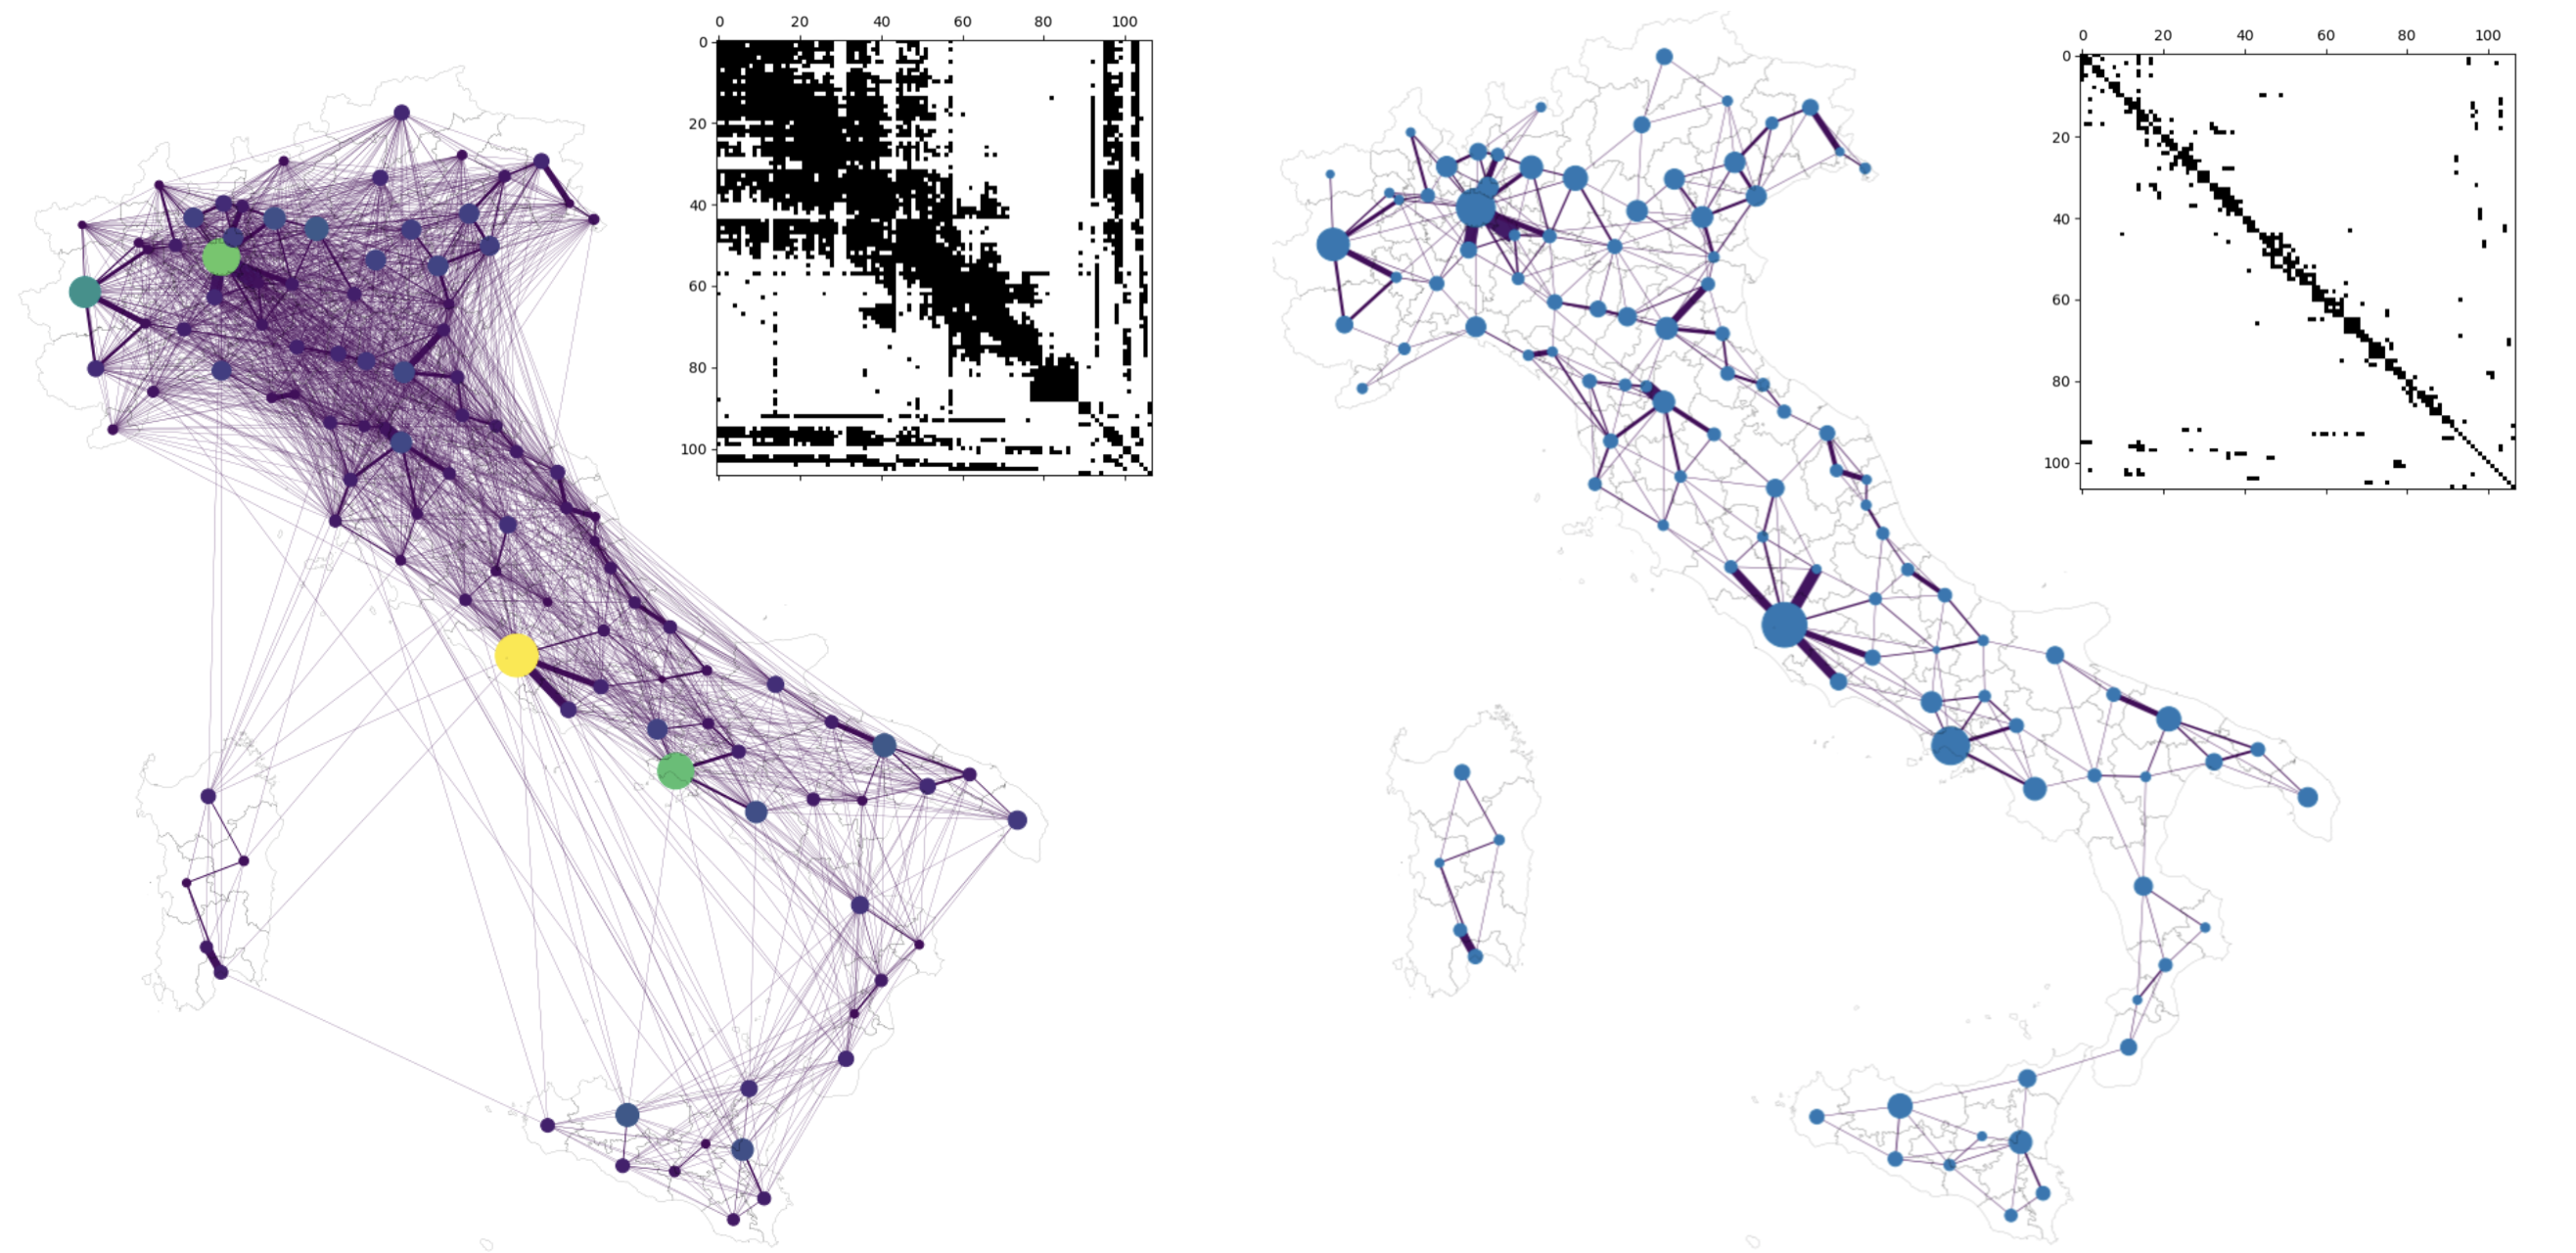
\includegraphics[width=\textwidth]{fig_italy-ocp/figuresSI/mobsimplification.png}
\caption[Simplification of the mobility matrix to obtain a sparse and tractable problem]{Simplification of the mobility matrix to obtain a sparse and tractable problem. After the optimization, the effectiveness of the optimal control strategy is assessed on the full model.} \label{figSI:mobility_simplification}
\end{figure*}

\paragraph{Possible further improvements} Applying optimal control in open loop, i.e., solving the optimization problem once and applying the control input over the whole time interval, may lead to poor performance due to model inaccuracy and external perturbations. A common remedy consists in closing the loop by repeatedly solving the OCP by using the most updated information on the initial states. This is the principle behind Model Predictive Control (MPC)~\cite{Rawlings:ModelPredictiveControl:2017}. In this context, the state would be estimated on a daily, weekly, or monthly basis so as to solve again the OCP and correct the optimal strategy.


%% ***********************************************************************************************
%\section{Data assimilation and model parameters}
%% ***********************************************************************************************
%\begin{figure*}
%    \centering
 %   \includegraphics[width=1\textwidth]{fig_italy-ocp/figuresSI/DA_all_sim/hosp.pdf}
  %  \caption[Modeled daily hospitalizations the against hospitalization data]{Modeled daily hospitalizations (blue) versus hospitalization data (red dots), regional detail of fig. 2.A in the main text. The optimistic and pessimistic transmission scenarios are represented in green and yellow, respectively.}
%    \label{fig:SI_DA1}
%\end{figure*}
%\begin{figure*}
%    \centering
%    \includegraphics[width=1\textwidth]{fig_italy-ocp/figuresSI/DA_all_sim/incidence.pdf}
%    \caption[Modeled daily incidence against the daily reported cases]{Modeled daily incidence (blue) versus the daily reported cases (red dots), regional detail of fig. 2.B in the main text. The optimistic and pessimistic transmission scenarios are represented in green and yellow, respectively.}
%    \label{fig:SI_DA2}
%\end{figure*}

%The regional transmission rates are the main parameters governing the force of infection of the model and, thus, the daily exposed individuals. To better track possible changes in the transmission rates, w- adopt a data assimilation strategy based on an iterative particle filter\cite{Manoli:IterativeParticleFilter:2015} used on a moving window of 14 days. The filter starts considering $N_r=1000$ model realizations at time $t_0$ (February 21, 2020), whose state variables are $x_0^{(j)}, j=1,\dots, N_r$, where the superscript $(j)$ is the realization index and the subscript is the temporal index. Each realization is associated with a parameter combination that is randomly sampled from the posterior distribution evaluated in\cite{Bertuzzo:GeographyCOVID19Spread:2020}, indicated with $\theta^{(j)}$. Possible spatial heterogeneities in regional transmission on a given day $t_k$ are obtained multiplying the transmission parameter by a coefficient $\phi_{k,i}^{(j)}$, where $i$ is the region's index. At time $t_0$, the coefficients $\phi_{0,i}^{(j)}$ are sampled from a truncated normal distribution (mean $\mu_0=1$, standard deviation 0.4, bounds $0.8\mu$-$1.2\mu_0$).
%At time $t_k$, w- assume to know the state variables $x_k^{(j)}$ and coefficients $\phi_{k,i}^{(j)}$, the latter having ensemble mean $\mu_{k,i}$. To update state variables and coefficients at time $t_{k+1}$, w- consider the observations (daily hospitalizations) collected in a temporal window of $\tau=14$ days, $(t_k,t_{k}+\tau$. New coefficients from the truncated normal distribution (mean $\mu_k=1$, standard deviation 0.4, bounds $0.8\mu_k$-$1.2\mu_k$) are sampled at time $\tau=t_0+14$ days.  For each realization, w- run the model during the window of 14 days, assuming that the coefficients change linearly for a week, from  $\phi_{0,i}^{(j)}$ to $\tilde{\phi}_{0,i}^{(j)}$, and remain constant afterwards.
%The regional likelihood of each realization is then evaluated during these two weeks considering that the daily hospitalizations follow a gamma distribution (as in\cite{Bertuzzo:GeographyCOVID19Spread:2020}). 
%A resampling step (systematic resampling , see, e.g.\cite{Douc:ComparisonResamplingSchemes:2005}) selects and duplicates the coefficients $\tilde{\phi}_{0,i}^{(j)}$ associated with the largest likelihood values. These coefficients are then used to update the mean value $\mu_k$. Finally, the simulation is repeated on the same temporal window by sampling new coefficients $\tilde{\phi}_{0,i}^{(j)}$ from the truncated normal distribution with the updated mean $\mu_k$. This set of coefficients is used to compute state variables and parameters at time $t_k$, and then as starting condition to produce the projections used in the main text.

%Model parameters (in the absence of vaccination) are taken from a paper\cite{Bertuzzo:GeographyCOVID19Spread:2020} where they were inferred in a Bayesian framework for the period February~24 -- May~1, 2020, on the basis of the official epidemiological bulletins released daily by Dipartimento della Protezione Civile\cite{DipartimentodellaProtezioneCivile:EmergenzaCoronavirusRisposta} (data available online at {\url{https://github.com/pcm-dpc/COVID-19}}) and the bulletins of Epicentro, at Istituto Superiore di Sanit{à}\cite{IstitutoSuperiorediSanita:CoronavirusUltimiAggiornamenti:2020,Palmieri:CharacteristicsCOVID19Patients:2020}. All the parameters estimated for the initial phase of the Italian \textsc{covid}-19 epidemic, including the transmission rates, are spatially homogeneous\cite{Bertuzzo:GeographyCOVID19Spread:2020}. This parameterization has been used to produce all the results presented in the main text.


%% ***********************************************************************************************
\paragraph{Spatial set-up} 
%% ***********************************************************************************************
The modeling tools described in the following sections are applied to the Italian \textsc{covid}-19 epidemic at the scale of second-level administrative divisions, i.e. provinces and metropolitan cities (currently, as of 2021, $107$ spatial units). Official data about resident population at the provincial level is produced yearly by the Italian National Institute of Statistics (Istituto Nazionale di Statistica, ISTAT; data available at\\ \url{http://dati.istat.it/Index.aspx?QueryId=18460}). The latest update (January 1, 2019) has been used to inform the spatial distribution of the population. %For the age-stratified model the data also comes from ISTAT, in the 2018 census: \url{http://demo.istat.it/popres/index.php?anno=2018&lingua=eng}.
The data to quantify nation-wide human mobility come from ISTAT (specifically, from the 2011 national census; data available online at \url{https://www.istat.it/it/archivio/139381}). Mobility fluxes, mostly reflecting commuting patterns related to work and study purposes, are provided at the scale of third-level administrative units (municipalities)\cite{Pepe:COVID19OutbreakResponse:2020,Vollmer:Report20Using:2020}. These fluxes were upscaled to the provincial level following the administrative divisions of 2019, and used to evaluate the fraction $p_i$ of mobile people in each node~$i$, as well as the fraction $q_{ij}$ of mobile people who move between~$i$ and all other administrative units~$j$ (see Supplementary Material in\cite{Gatto:SpreadDynamicsCOVID19:2020}).
The epidemiological data is obtained from the bulletins of the Dipartimento della Protezione Civile, \url{https://github.com/pcm-dpc/COVID-19}).

%% ***********************************************************************************************
\section{Details of the alternative strategies}
%% ***********************************************************************************************
Alternative strategies are created to be compared the optimal solutions. Each strategy uses a decision variable, $\mathcal{V}_i$, as a basis for the allocation of vaccines among provinces. The decision variable is one of:
\begin{itemize}
    \item \textsc{modelled future incidence, absolute}: the modelled total future incidence in a no-vaccination scenario. This is equivalent to the objective of the optimal control problem with no control;
    \item \textsc{modelled future incidence, per population}: as above, but normalized by the resident population in each node;
    \item \textsc{modelled initial susceptibility, absolute}: the modelled number of susceptibles in each province at the start of the vaccination campaign;
    \item \textsc{modelled initial susceptibility, per population}: as above, but normalized by the resident population in each node;
    \item \textsc{province's population}.
\end{itemize}

Two strategies to distribute the doses are defined:
\begin{itemize}
\item \textsc{Focused} Where every province is sorted (higher on top) according to its decision variable $\mathcal{V}_i$. The maximum local rate $v_i^{max}$ is allocated to every province going down through the list, until the stockpile is empty. In other words, assuming an amount $K$ of vaccines is available in the stockpile, the province index $i$ that satisfy $\max_i \mathcal{V}_i$ is searched for, and province $i$ is assigned $M_i = \min(v_i^{max}, K)$ vaccines. Then, the next province $j$ that satisfy $\max_{j,j\neq i} \mathcal{V}_j$ is searched for and assigned $M_j = \min(v_j^{max}, K-M_i)$. And so on, until no vaccine remains in the stockpile. This strategy will concentrate the allocation on nodes with the highest values of the considered decision variable.
\item \textsc{Proportional} In this case, assuming that on a given day there is a quantity of vaccine $K$ in the stockpile, each province $i$ receives an amount $M_i = \min(v_i^{max}, K \cdot \frac{\mathcal{V}_i}{\sum_j \mathcal{V}_j})$. This approach vaccinate each node proportionally to the value of its decision variable $\mathcal{V}_i$.
\end{itemize}
In the main text, the results for three alternative strategies are shown, namely \textit{proportional absolute incidence}, \textit{proportional population}, and \textit{proportional susceptibility}---named respectively Incidence, Population, and Susceptibility. These strategy are good performers across scenarios, and show how different choices for the decision variables may affect the outcomes of the OCP. In the next sections, the results for all these alternative strategies are shown.

%% ***********************************************************************************************
\section{Additional results}
%% ***********************************************************************************************
The results for all these strategies is presented in tab.~\ref{table:all_strat}, and are shown side-by-side in fig.~\ref{fig:OC_comparison_all}. The optimal solutions outperforms all the others solution. In fact, for every given posterior realisation, the optimal control solution always outperforms all other allocation strategies. Even if some scatter is observed when sampling the posterior, the performances of optimal strategies are clearly separated from the rest of the alternatives.

A linear scatter plot of the optimal proportion of vaccinated individuals per province (sorting variable) side by side with the province population, the projected incidence without vaccination, and the proportion of susceptible individuals at the start of the simulation is presented ro further investigate the features of the optimal solution. These results are presented for the optimistic scenario in fig.~\ref{fig:OC_scatter_optimistic} and for the pessimistic scenario in fig.~\ref{fig:OC_scatter_pessimistic}. No clear visual pattern associating these covariates to the optimal proportion vaccinated is found, highlighting again that the optimal allocation uses the epidemiological variable in a non-straightforward way, different from every simple strategy designed for this exercice.

\begin{fwtable}
\centering
\small
\begin{tabular}{llrrrr}
\toprule
& {} & \multicolumn{2}{c}{Averted Infections} & \multicolumn{2}{c}{Averted Infections} \\
&    &  & & \multicolumn{2}{c}{per dose} \\
Scenario & Method &  Optimistic & Pessimistic &     Optimistic & Pessimistic          \\
\midrule
2M & Optimal &   6.98M &    30.6M &          0.268 &        1.18 \\
        & Incidence &   6.32M &    28.1M &          0.243 &        1.08 \\
        & Proportional Incidence &   6.23M &    27.5M &          0.239 &        1.06 \\
        & Focused Susceptibility &   6.03M &    26.9M &          0.232 &        1.03 \\
        & Focused Proportional Susceptibility &   6.03M &    26.9M &          0.232 &        1.03 \\
        & Focused Proportional Incidence &   6.03M &    26.9M &          0.232 &        1.03 \\
        & Focused Population &   6.03M &    26.9M &          0.232 &        1.03 \\
        & Focused Incidence &   6.03M &    26.9M &          0.232 &        1.03 \\
        & Population &   6.02M &    26.8M &          0.231 &        1.03 \\
        & Susceptibility &   5.97M &    26.7M &          0.229 &        1.02 \\
        & Proportional Susceptibility &    5.6M &    25.3M &          0.215 &       0.971 \\
1.5M & Optimal &   5.52M &    24.1M &          0.283 &        1.24 \\
        & Incidence &   4.89M &    21.7M &           0.25 &        1.11 \\
        & Proportional Incidence &   4.82M &    21.3M &          0.246 &        1.09 \\
        & Focused Population &   4.58M &    20.5M &          0.235 &        1.05 \\
        & Focused Incidence &   4.58M &    20.5M &          0.235 &        1.05 \\
        & Focused Proportional Incidence &   4.58M &    20.5M &          0.235 &        1.05 \\
        & Focused Proportional Susceptibility &   4.58M &    20.5M &          0.235 &        1.05 \\
        & Focused Susceptibility &   4.58M &    20.5M &          0.235 &        1.05 \\
        & Population &   4.57M &    20.4M &          0.234 &        1.05 \\
        & Susceptibility &   4.51M &    20.3M &          0.231 &        1.04 \\
        & Proportional Susceptibility &   4.18M &     19.0M &          0.214 &       0.975 \\
1M & Optimal &    3.9M &    16.9M &            0.3 &         1.3 \\
        & Incidence &   3.41M &    15.1M &          0.262 &        1.16 \\
        & Proportional Incidence &   3.34M &    14.7M &          0.257 &        1.13 \\
        & Focused Population &   3.09M &    13.9M &          0.238 &        1.07 \\
        & Focused Susceptibility &   3.09M &    13.9M &          0.238 &        1.07 \\
        & Focused Proportional Susceptibility &   3.09M &    13.9M &          0.238 &        1.07 \\
        & Focused Incidence &   3.09M &    13.9M &          0.238 &        1.07 \\
        & Focused Proportional Incidence &   3.09M &    13.9M &          0.238 &        1.07 \\
        & Population &   3.08M &    13.8M &          0.237 &        1.06 \\
        & Susceptibility &   3.02M &    13.7M &          0.232 &        1.05 \\
        & Proportional Susceptibility &   2.75M &    12.6M &          0.211 &       0.972 \\
479'700 & Optimal &   1.96M &    8.39M &          0.314 &        1.34 \\
        & Focused Proportional Incidence &   1.95M &    7.74M &          0.312 &        1.24 \\
        & Proportional Incidence &   1.69M &    7.32M &          0.271 &        1.17 \\
        & Incidence &   1.63M &    7.21M &          0.262 &        1.15 \\
        & Focused Incidence &   1.59M &    6.64M &          0.254 &        1.06 \\
        & Focused Population &   1.57M &    6.85M &          0.251 &        1.09 \\
        & Population &   1.45M &    6.57M &          0.233 &        1.05 \\
        & Focused Susceptibility &   1.45M &    6.53M &          0.232 &        1.04 \\
        & Susceptibility &   1.41M &    6.43M &          0.225 &        1.03 \\
        & Focused Proportional Susceptibility &   1.28M &    6.09M &          0.204 &       0.973 \\
        & Proportional Susceptibility &   1.26M &    5.89M &          0.202 &       0.944 \\
\bottomrule
\end{tabular}
\caption{Absolute number of averted infections for each scenario}
\label{table:all_strat}
\end{fwtable}

\begin{fwfigure}
    \centering
    \includegraphics[width=0.9\textwidth]{fig_italy-ocp/figuresSI/scenarios_perturb_all_SI.pdf}
    \caption[Comparison of different allocation strategies]{Comparison of different allocation strategies. Percentages of averted infections per vaccine dose from January 11, 2021 to April 11, 2021 using different vaccine distribution strategies for the pessimistic (panel A) and the optimistic (panel B) scenario based on: the optimal solution, the spatial distribution of the population, the amount of susceptible individuals at the beginning of the vaccination campaign, and the projected disease incidence in the absence of control. A median realization of the modeled posterior is optimized (diamonds), and the performance is assesed on the whole posterior (box plots). The results are normalized by the number of averted infections in the optimized solution (see tab.~\ref{table:all_strat} for absolute values).}
    \label{fig:OC_comparison_all}
\end{fwfigure}


\begin{figure}[!ht]
    \centering
    \includegraphics[width=\textwidth]{fig_italy-ocp/figuresSI/SI_scatter_Optimistic.pdf}
    \caption[Control and co-variates for the optimistic scenario]{Control and co-variates for the optimistic scenario with a stockpile delivery of 479'700 vaccine doses.}
    \label{fig:OC_scatter_optimistic}
\end{figure}

\begin{figure}[!ht]
    \centering
    \includegraphics[width=\textwidth]{fig_italy-ocp/figuresSI/SI_scatter_Pessimistic.pdf}
    \caption[Control and co-variates for the pessimistic scenario]{Control and co-variates for the pessimistic scenario with a stockpile delivery of 479'700 vaccine doses.}
    \label{fig:OC_scatter_pessimistic}
\end{figure}

%\begin{figure}[!ht]
%    \centering
 %   \includegraphics[width=\textwidth]{fig_italy-ocp/figuresSI/SI_all_states.pdf}
  %  \caption[Example of the dynamics in all compartments]{Example of the dynamics in all compartments for every node in the pessimistic scenario with a stockpile delivery of 479'700 doses. The lower right plot shows the control variable, the number of doses per day in each province.}
%    \label{fig:OC_ts_all}
%\end{figure}






% %%%%%%%%%%%%%%%%%%%%%%%%%%%%%%%%%%%
% %%%%%%%%%%%%%%%%%%%%%%%%%%%%%%%%%%%
% %%%%%%%%%%%%%%%%%%%%%%%%%%%%%%%%%%%
% %%%%%%%%%%%%%%%%%%%%%%%%%%%%%%%%%%%
\chapter[Materials and methods]{Materials and methods} %(Computational epidemiomology or Infectious Disease Modeling

%\section{Infectious Diseases Epidemics} %as a phenomena 
Infect

\section{Modeling of Epidemics}
Modeling has several purposes:
The ultimate goal being  the forecasting and estimating the propagation of uncertainties from the observable past to the future. control

Alongside, modeling helps us to understand the different processes of the cholera life cycle. 

As a substitute for physical experiments, different mechanistic pathways can be compared by benchmarking them against the reproduction of reported cases. 

Models may have only one spatial dimension or may consider the spatial spread of the epidemic across several nodes. Spatially-explicit mathematical models provide key insights into the course of an ongoing epidemic, where transmission is heterogeneous in space and time.

% (Bayesian philosophy, data, representation of reality) sochastic/determistic Modeling of epidemics (uncertainties, social factors, heterogeneities)


In the next part of this chapter, we present so

\subsection{Data}
%data on health
Model makes use of epidemiological data: reported cases, severity of outcomes, serology survey. 

Covariates or input data range from rainfall and temperature, human mobility.

Information and prior on



\subsection{Model design}


The cornstone of epidemiological modeling is the compartmental model. Individuals belongs to compartiments who caraterize their stage with respect to the disease. The seminal work has introduced compartiments for Susceptible, Infected, Recovered. The SIR model, first introduced first by Kermack and McKendrick\cite{Kermack:ContributionMathematicalTheory:1927}. 

Or

An Exposed compartiment may be added 
Compartimental + spatially explicit

\paragraph{Transitions}



\paragraph{Residence time}

\cite{Hurtado:GeneralizationsLinearChain:2019}

\marginnote{It’s also possible to approximate a non-Erlang delay distribution with a mixture of Erlang distribution \parencites[Appendix 4]{Hurtado:GeneralizationsLinearChain:2019}.}

\subsection{Inference and calibration} 
Model parameters in the SIRB cholera models represent physical rates. However, in the literature there is no consensus on their values or on their  probability distribution. Numerical calibration is therefore required to assess their value in any particular application. Parameter identifiability is one of the major problems during the calibration of SIR-like epidemiological models. This is mainly due to the impossibility to directly measure the exact figures of individual infections in each compartment, the uncertainty associated to epidemiological data and the net effect of possible model over-parametrization. Calibration thus often results in combination of parameters that produce almost identical fits, termed equifinality\footnote{For a cholera example, Eisenberg et al. (\fullcite{eisenberg_identifiability_2013}) highlighted that the presence of uncertain measurements might generate strongly correlated parameters, which cannot be unambiguously identified.}.

\paragraph{Iterated Filtering}




\paragraph{Markov-Chain Monte Carlo}



\paragraph{Estimation of $R_0$} 

 Filtering
\subsection{Evaluation}
We may evaluate thte model predictive accuracy
\subsection{Model Selection}
% DONE w.r.t gelman
% TODO w.r.t McElreath
For inference or prediction, several candidates models may be devised for same data and process. Model selection aims at finding the \textit{best} (set of) model(s) for the task at hand. In the perspective of identifying the data-generating process a consistent model selection criteria is warranted\parencite{Hoge:PrimerModelSelection:2018}.  On way of doing that is to compare their predictive accuracy. Sometime it can be computed in way that is tailored to the application and embed the benefits and cost of predictiding data with the model \footnote{i.e for weather, predicting rain when there’s none is considered lower cost than predicting sun when it rains}, or we may resort to generic rules.
The log-likelyhood (or log predictive density), $\Pr(data \mid \boldsymbol\theta$  is often used. Note by using the likelyhood instead of the posterior, we don’t depends on the priors but just on the data model (but as the prior influence $\boldsymbol\theta$, it does affects the calculation of the predictive density). The log predictive accuracy as a scoring function i related to information theory, and to the Kull-back Leibler information.
Unfortunatly, the hypothetical gold standard that is the expected log predictive density for new datapoints is out-of-reach in most of our problems. However we can compute an optimistic\footnote{optimistic because we have used the same as we used to calibrate our model. Generaly, out-of-sample predictions (i.e for a new datapoint) will be less accurate that what this within-sample accuraty}estimation, computing the log-poinwise predictive density of our model to the fitted data. For $s$ posterior samples and our $n$ datapoints, we have
\begin{equation}
	EQUN 7.4~\label{eq:llik}
\end{equation}
To approxmimate the true out-of sample predictive accurcy we can 
\begin{itemize}
	\item Fit the model to a part (a fold) of the available data and compute it’s predictive accucary on the other part. This is called \emph{cross-validation}, and a common version of it is leave-one-out cross validation, where, in turn we leave out just one datapoint for calibration and compute the predictive accuacy on it. This is computationally expensive, as we need to perform $n$ calibrations.
	\item Hence many methods where designed to unbias the within-sample accuracy and approximate the results of cross-validation, usually by substracting  a correction made of some functions for the effective parameters being fit. We find here an alphabet of information criterions (ICs):  Akaike (AIC), Deviance  (DIC), Watanabe-Akaike (WAIC)\footnote{AIC takes into consideration the number of parameters while DCI, WAIC compute aneffective number of parameters that takes into account the observed data. While the means are different,  all estimating the same thing: the expected out-of-sample deviance associated with a model. BIC, introduced futher, is notably different because as its goal is different: estimating the marginal probabability of the the data under the model and is related to the bayes factor, see below.} being notable.
\end{itemize}
And both of these methods penalize overfitting (more paramters always improve fit), as they assess the generality of the model.




. Within each family of deterministic and stochastic models, we employ both Bayesian (Bayes Factors, BFs) and frequentist (likelihood ratio tests) model comparison techniques. 

For the deterministic model, calibrated using Bayesian inference, we use the Bayes Factors (BFs). Bayes Factors are a controversial\footnote{See the great debate in Sociological Methodology:\fullcite{Raftery:BayesianModelSelection:1995} and counter arguments\fullcite{Gelman:AvoidingModelSelection:1995}} method that we use in our XXX chapter to compare discrete choices of model.

We have a model selection problem. Given the observation of data $D$, we have to choose between two models $\mathcal{M}_i$ and $\mathcal{M}_j$ each parametrized by parameters sets $\theta_i$ and $\theta_j$.

\paragraph{Bayes Factor}  The goal might be to choose on of the model or to averates discrete set of probabilites. The aim is to link the posteriors and prior odd ratios:
\begin{equation}
    \overbrace{\frac{\mathbb{P}(\mathcal{M}_i\mid D)}{\mathbb{P}(\mathcal{M}_j\mid D)}}^{\text{posterior odd ratio}} =
    \overbrace{BF_{i,j}}^\text{Bayes factor} \times  \overbrace{\frac{\mathbb{P}(\mathcal{M}_i)}{\mathbb{P}(\mathcal{M}_j)}}^{\text{prior odd ratio}}
\end{equation}
 where $\mathbb{P}(\mathcal{M}\mid D)$ represents the posterior probability of a model $\mathcal{M}$ is the probability of the model given the data
Given Bayes theorem, we have
\begin{equation}
  BF_{i,j} = \frac{\mathbb{P}(D\mid\mathcal{M}_i)}{\mathbb{P}(D\mid\mathcal{M}_j)}
\end{equation}
 where $\mathbb{P}(D\mid\mathcal{M})$ is  the \textit{model evidence}, or marginal likelihood of model $\mathcal{M}$ \parencite{Aitkin:PosteriorBayesFactors:1991}. It represents the probability of the data given the model, not assuming any particular model parameters (because parameter $\theta$ have been \textit{marginalized (integrated) out}), and is given by a (difficult to compute) integral:
 \begin{equation}
\mathbb{P}(D\mid\mathcal{M}) = \int_\theta \mathbb{P}(D\mid\theta,M) \mathbb{P}(\theta\mid M) d\theta .
\end{equation} 
 The model evidence can be directly computed using the output the mcmc algorithm as the harmonic mean of each model likelihood over the posterior distribution of the parameters. As described by\textcite{Weinberg:ComputingBayesFactor:2012}, if one can draw $N$ samples from the posteriors of the parameters, $\theta^{(i)} \sim \mathbb{P}(\theta\mid\mathcal{M}, D)$, a Monte Carlo estimate of the model evidence is given by:
 \begin{equation}
 	\mathbb{P}(D\mid\mathcal{M}) \approx {\left[ \frac{1}{N} \sum_{i=1}^N \frac{1}{\underbrace{\mathbb{P}(D\mid\theta^{(i)})}_{\text{likelyhood of } \theta^{(i)}}} \right]^{-1}}, 
 \end{equation}
which can then be used to derive BFs (see \parencite{Raftery:EstimatingIntegratedLikelihood:2007} for a discussion on the possible numerical issues involved in this approximation.
%\end{multicols}

%\begin{multicols}{2}
 \paragraph{Bayesian Information Criterion} On the other hand, model evidence of the stochastic model was evaluated using the Bayesian Information Criterion (BIC) computed at the Maximum Likelihood Estimate (MLE) resulting from the multiple itertated filtering algorithm (see section~\ref{sec:calibration}). BIC enables the estimation of the BFs as $BF_{i,j} \approx e^{\frac{1}{2}(BIC_j - BIC_i)}$ yielding the relative support of each $\mathcal{M}_i$ against $\mathcal{M}_j$ \parencite{Schwarz:EstimatingDimensionModel:1978a,Burnham:MultimodelInferenceUnderstanding:2004}. 
 
  \paragraph{Likelyhood ratio tests} Since the set of models we consider here are nested, we additionally perform likelihood ratio tests (LR-tests) to determine the significance of incorporating additional transmission processes on top of the basic SIRB formulation. LR-tests were implemented by sequentially\footnotemark{} relaxing the constraint that the human-to-human and rainfall-related parameters are equal to 0 in \textbf{MN}. More particularly, we perform a LR-test for each pair of models $\{\mathcal{M}_0, \mathcal{M}_1\}$ who’s parameter vectors $\boldsymbol{\theta}^0,\boldsymbol{\theta}^1$ take values from the set of all possible values in the parameter space $\Theta \subset \mathbb{R}^{n_p}$, for which at least on of the parameters that is not null is $\boldsymbol{\theta}^1$ is equal to 0 in $\boldsymbol{\theta}^0$, i.e.  $\boldsymbol{\theta}^0 \in \Theta^0 \subset \Theta, \boldsymbol{\theta}^1 \in \Theta^1 \subset \Theta, \Theta^0 \subset \Theta^1 = \Theta \setminus \Theta^0$, with $\Theta^0 = \{ \boldsymbol{\theta} \mid \{\theta_1, \dots, \theta_p  \} \in \mathbb{R}^{n_p} \wedge \ \exists i \in \{1,\dots, p\} : \theta_i = 0 \} $.
%Taken including the Bayesian Information Criterion (BIC)~ and a the . BIC is a criterion which penalizes the best log-likelihood computed during calibration by the model complexity (in this case, the number of parameters $n_p$) thus allowing to compare models having different degrees of freedom. DIC is particularly suited for Bayesian model selection when using an \textsc{mcmc} approach. DIC considers the average ensemble deviance associated to the posterior trajectories and penalizes it by its variance. Finally the likelihood-ratio test (LR test) is a statistical test to evaluate if the increase of complexity among two nested models is convenient with respect to the improvement of the fit (increase of the log-likelihood).
%\end{multicols}




 \section{Control of epidemic, and modeling of control of epidemics}%Public-health decision making tools using models
%- Control of epidemic, and modeling of control of epidemics
%- Public-health decision making tools using models



\subsection{Optimal control}
%%%%%%%%%%%%%%%%%%%%%%%%%%%%%%%%%%%%%%%%%%%%%%%%%%%%%%%%%%%%%%%%%%%%%%%%%%%%%%%%%%%%%%%%%%%% OK
\paragraph{Optimal Control Theory}
Optimal control theory describes the application of control variables to a system for the purpose of maximizing some measure of performance. The system is subject to its dynamics, with possible constraints on state and control variables. Let $\textbf{x}(t)$ be the state of a system at time $t$, and $\textbf{u}(t)$ be the control (or input) variable. 

In the general form, a continuous time optimal control problem (OCP) is written as the minimization of a cost functional $J$  with respect to the control variable $u(t)$:
\begin{equation}
\text{Minimize~~~} \min_{u(\cdot)} J=\Phi\,[\,\textbf{x}(t_0),t_0,\textbf{x}(t_f),t_f\,] + \int_{t_0}^{t_f} \mathcal{L}\,[\,\textbf{x}(t),\textbf{u}(t),t\,] \,dt
\end{equation}
subject to the system dynamics, path constraints and boundary conditions:
\begin{align}
\dot{\textbf{x}}(t) & =  \textbf{g}\,[\,\textbf{x}(t),\textbf{u}(t),t\,] \eqname{System dynamics}\\
\textbf{b}\,[\,\textbf{x}(t),\textbf{u}(t),t\,]  & \leq  \textbf{0} \eqname{Path constraints} \\
\boldsymbol{\phi}\,[\,\textbf{x}(t_0),t_0,\textbf{x}(t_f),t_f\,] & =  0 \eqname{Boundary conditions} 
\end{align}

The objective $J$ is the sum of the endpoint cost function $\Phi$ and the so called Lagrangian functional $\mathcal{L}$ that represent the cost along the path followed by the system.

The first constraints of the system are its dynamics, here a general ordinary differential equation $\textbf{g}$. In the case of cholera application, this is the spatially-explicit SIRB model. Path constraints $\textbf{b}$ in the form of inequalities are said inactive, and may be active when imposed as equalities. Finally, boundary conditions allow for forcing the system to end in a certain state, and to specify initial conditions.

Note that it is also possible to optimize the end time $t_f$. A simple change of variable transforms the OCP above into a free-end time problem. This possibility might result fundamental to optimize for the time of cholera extinction.

%%%%%%%%%%%%%%%%%%%%%%%%%%%%%%%%%%%%%%%%%%%%%%%%%%%%%%%%%%%%%%%%%%%%%%%%%%%%%%%%%%%%%%%%%%%% OK
\paragraph{Solving an Optimal Control Problem}
Solving an OCP is a difficult task, but it  has received large attention during the cold war to guide rockets and missiles. Except for simple problems, like the linear quadratic  control, OCPs do not have analytical solutions and numerical solutions are typically sought. We highlight here two general methods for solving OCPs:

\par Indirect methods (or ``optimize then discretize’’) use the calculus of variation to obtain first-order optimal conditions. The OCP is transformed in a multi-point boundary value problem (BVP) that has the form of a Hamiltonian system. Pontryagin’s maximum principle guarantees the optimality of the solution. While this solution is elegant, the BVP may be difficult to solve and recently, direct methods are frequently preferred in applications.

\par The rational behind direct (or ``discretize then optimized’’) methods is that a nonlinear programming (NLP) optimization problem with large dimension (tenth of thousand variables) has an easier numerical solution than a simple BVP, because it is sparse. That is, we rewrite our OCP (in the infinite dimensional functional space) into an optimization NLP (in a finite dimensional Euclidean space). 

In short, state and control variables are approximated (e.g using a piece-wise constant function) and the cost functional becomes a cost function. The problem is now to find the coefficients defining the control variable approximation, in such a way that they minimize the approximated cost function $F$. This leads to the following NLP:
\begin{equation}
\min_{\textbf{x} \in \mathbb{R}^n} F(\textbf{x})
\end{equation}
subject to:
\begin{equation}
g(\textbf{x}) = 0
\end{equation}    
\begin{equation}
h(\textbf{x}) \leq 0
\end{equation}
This problem is solved by any NLP solver, like Ipopt~\cite{wachter_implementation_2006}.   Optimal control toolboxes, like CasADI~\cite{andersson_casadi:_2012}, allow us to transform the symbolic formulation of the OCP in into an NLP. 

Despite a wide range of power tools, solving even a simple  optimal control problem is still a computationally-intensive task.

\paragraph{Epidemiological Applications of Optimal Control}

Optimal control is of great interest for practitioners and policy makers: it allows to formally back up existing policies, and may suggest alternative action plans. Indeed, such discoveries have to be carefully analyzed in order to be understood, as they might be due to model features. We present a brief literature review of studies on optimal control for epidemiological applications. This non-exhaustive review should present a sufficient picture of the current research landscape.

First, theoretical studies\cite{kar_stability_2011, laguzet_global_2015} on  generic epidemiological models explored the feasibility and features of optimal control polices. These studies, first by Morton and Wickwire\cite{morton_optimal_1974}, Sethi and Staats\cite{sethi_optimal_1978}, Greenhalgh\cite{greenhalgh_results_1988}, Behncke\cite{behncke_optimal_2001} analyzed  various spatially-implicit models in a control system perspective, deriving existence, uniqueness, and stability of the optimal control for some (ideal) inputs like quarantine and vaccination.

It is also possible to use optimal control in order to find some general rules for disease intervention. For example, Rowthorn \textit{et al.}~\cite{rowthorn_optimal_2009} showed that for a system with two interconnected regions and a particular epidemic, equalizing infection in the two regions is the worst possible strategy in minimizing the total number of infection.

For cholera, intervention considered are a combination of antibiotics, vaccination and WaSH improvement. Tuite \textit{et al.} applied optimal control to the 2010 Haitian epidemic. For spatial allocation of the (rather small) vaccine stockpile available at that time, they compared optimal allocation against equal and density-dependent. They found that the later the vaccination is done, the better the optimal allocation performs against the control allocation strategies~\cite{tuite_cholera_2011}. However, there a few caveat in this study like the lack of inapparent infections~\cite{king_inapparent_2008, rinaldo_reassessment_2012}. Another approach was undertaken by Neilan \textit{et al.}~\cite{millerneilan_modeling_2010} in Calcutta and Bogra. They optimized for rehydratation/antibiotics, vaccination and sanitation, and concluded that a problem dependent mix of these methods is the most effective intevention strategy. This last approach and many others~\cite{sardar_optimal_2013} are designed for spatially-implicit models, and optimize the timing and proportion of the different interventions.

In an interesting theoretical study, Kelly Jr. \textit{et al.}~\cite{kelly_impact_2016} explored different mobility patterns and  optimal control intervention strategies. Namely, they tested a spatially-explicit version of the Tien and Earn model~\cite{tien_multiple_2010} and different spatial setups: nearest-neighbour connectivity, hub arrangement, and  hotspot map. They derived vaccination strategies. For example, one non-intuitive finding is that for nearest-neighbour connectivity, the outbreak patch should receive the least amount of effort.  A study by Chao \textit{et al.} compared different vaccination strategies using a spatially explicit model at small scale~\cite{chao_vaccination_2011}.  

Other cholera control analysis are either conceptual (no data nor a particular setup)~\cite{fister_optimal_2016} or do not search for an optimal control solution, but test the impact of different possible  strategies~\cite{kirpich_controlling_2017, eubank_modelling_2004, finger_potential_2018, seidlein_preventing_2018,azman_micro-hotspots_2018,lessler_mapping_2018,rebaudet_dry_2013}.

These studies are either theoretical, without connection to a particular setup nor actual data, or compare different control strategies defined by the author. In the framework of this thesis, I aim to develop a computational tool able to solve the optimal control problem for actual cholera outbreaks in quasi-real time, in order to provide objective information that can promptly support the health-care actors during the emergency. 


\end{appendices}
%\begin{fullwidth}\printbibliography\end{fullwidth}

\end{document}